% For printing in a4
%\documentclass[a4,10pt,twoside,openright,italian,english]{book}% twoside!

% For printing with the A5 format
\documentclass[10pt,twoside,openright,english,italian]{book}% twoside!

% Set paper size
\usepackage[twoside=true]{geometry}

%For printing with the weird format
%\geometry{
%	paperwidth=17cm,
%	paperheight=24cm,
%	margin=2cm,
%	top=2.3cm,
%	bindingoffset=0.4cm
%}
% For printing in a4
 \geometry{a4paper,
  margin=3cm,
  top=3.8cm,
  bindingoffset=0.4cm
 }

%Uncomment this for final prints: this just enables printing on a4 paper
\usepackage[cam,center,a4,pdflatex,axes]{crop}

\usepackage{phdthesis}

\usepackage{fancyhdr}
\usepackage{color}
\usepackage{array}
\usepackage{mdwmath}
\usepackage{mdwtab}
\usepackage{amsmath,amssymb}
\usepackage{cite}
\usepackage{graphicx}
\usepackage{glossaries}
\usepackage{listings}
\usepackage{subfig}
\usepackage{booktabs}
\usepackage{latexsym}
\usepackage{url}
\usepackage{bnf}
\usepackage{rotating}
\usepackage{multirow}
\usepackage{phdtitle}
\usepackage{paralist}
\usepackage{bibentry}
\usepackage{xcolor}
\usepackage{enumitem}
%\usepackage[algochapter]{algorithm2e}
\usepackage[bookmarks=true,pdftex=false,bookmarksopen=true,pdfborder={0,0,0}]{hyperref}
\usepackage{lscape}
\usepackage{algorithmic}
\usepackage{algorithm}
\usepackage{longtable}
\usepackage[T1]{fontenc} 
\usepackage[latin1]{inputenc}
\usepackage[official]{eurosym}

%Custom package
\usepackage{amssymb}
\usepackage[full]{textcomp}
\usepackage{lmodern}
\usepackage{lineno}
\setcounter{tocdepth}{3}
\usepackage{float}
\usepackage{booktabs}
\usepackage{color}
\usepackage[verbose]{placeins}
\usepackage{blindtext}
\usepackage{makecell}
\usepackage{amsfonts}
\usepackage{colortbl}
\usepackage{tabulary}
\usepackage{etoolbox}
\usepackage{courier}
\usepackage{stix}

%\setlist{nosep}

%% \hyphenation{} is used to force the 
\hyphenation{}

\newtheorem{Definition}{Definition}[section]
\newtheorem{Example}{Example}[section]

\lstset{tabsize=2,basicstyle=\footnotesize,breaklines=true}

%%Custom listing styles
\lstdefinestyle{RDF}{
    numbers=left,                
    numberstyle=\scriptsize,
    tabsize=4,
    rulecolor=,
    language=xml,
    basicstyle=\ttfamily\footnotesize,
    aboveskip={1\baselineskip},
    columns=fixed,
    showstringspaces=false,
    extendedchars=true,
    breaklines=true,
    prebreak = \raisebox{0ex}[0ex][0ex]{\ensuremath{\hookleftarrow}},
    frame=single,
    showtabs=false,
    showspaces=false,
    showstringspaces=false,
    identifierstyle=\ttfamily,
    keywordstyle=\ttfamily,
}

\lstdefinestyle{N3}{
  basicstyle=\ttfamily\footnotesize,
  numberblanklines=true, 
  morekeywords={@prefix},
  %morekeywords={frappe,frEvent,frCell,frPixel,frFrame,frPlace,frGrid,frInstant,frCapture,frContent,frAct,frAgent,frEntity,xsd,prov,event,rdfs,time},
  frame=single
}

\lstdefinestyle{SPARQL}{
  basicstyle=\ttfamily\footnotesize,
  numberblanklines=true,
  morekeywords={PREFIX,AS,FROM,SELECT,CONSTRUCT,FROM,WHERE,COUNT,SUM,AVG,DISTINCT,FILTER,GROUP,ORDER,BY,ASC,DESC},
  frame=single
}

\lstdefinestyle{CSPARQL}{
  basicstyle=\ttfamily\footnotesize,
  numberblanklines=true,
  morekeywords={PREFIX,REGISTER,STREAM,AS,FROM,SELECT,CONSTRUCT,FROM,RANGE,STEP,WHERE,COUNT,SUM,AVG,DISTINCT,FILTER,GROUP,ORDER,BY,ASC,DESC},
  frame=single
}

\lstdefinestyle{ESPER}{
  basicstyle=\ttfamily\footnotesize,
  numberblanklines=true,
  morekeywords={SELECT,FROM,SUM,WIN,TIME_BATCH,TIME,EXT_TIMED_BATCH,GROUP,BY,OUTPUT,SNAPSHOT,EVERY,FORCE_UPDATE,START_EAGER,MAX,HAVING,COUNT,istream,rstream,irstream},
  frame=single
}

\lstdefinestyle{JSON}{
  basicstyle=\ttfamily\footnotesize,
  numberblanklines=true,
  morekeywords={@context,@type,@type,@id},
  frame=single
}

\lstdefinestyle{SPARKSQL}{
  basicstyle=\ttfamily\footnotesize,
  numberblanklines=true,
  morekeywords={PREFIX,REGISTER,STREAM,AS,FROM,SELECT,CONSTRUCT,FROM,RANGE,STEP,WHERE,COUNT,SUM,AVG,DISTINCT,FILTER,GROUP,ORDER,BY,ASC,DESC,WINDOW,ON,EVERY,LEFT,JOIN},
  frame=single
}

\lstdefinestyle{SPARKCODE}{
  basicstyle=\ttfamily\footnotesize,
  numberblanklines=true,
  morekeywords={$,val,groupBy,window,Agg,Count,count},
  frame=single
}

\lstdefinestyle{JSONIQ}{
  basicstyle=\ttfamily\footnotesize,
  numberblanklines=true,
  morekeywords={FOR,COLLECTION,GROUP,BY,RETURN,COUNT,IN},
  frame=single
}

\usepackage[greek,english,italian]{babel}

\usepackage{ulem}
\normalem

\hypersetup{pdftitle={Title}, pdfauthor={Author}}

\nobibliography*

\department {Dipartimento di Elettronica, Informazione e Bioingegneria}
\phdprogram{Doctoral Programme In Information Technology}

\author{Marco Balduini}
\title{On the Continuous and Reactive Analysis of a Variety of Spatio-Temporal Data}
\supervisor{Emanuele Della Valle}
\tutor{Stefano Ceri}
\advisor{Andrea Bonarini}
\titleimage{img/logopoli.png}
\phdcycle{2018 -- XXX Cycle}

% Custom command
\newcommand{\frappe}{FraPPE} 
\newcommand{\sti}{Natron}
\newcommand{\hivedi}{rvr@Hive}
\newcommand{\sparkdi}{rvr@Spark}
\newcommand{\kafkadi}{rvr@Kafka}
\newcommand{\river}{RI\rotatebox[origin=c]{90}{V}E\reflectbox{R}}
\def\ojoin{\setbox0=\hbox{$\bowtie$}%
  \rule[-.02ex]{.25em}{.4pt}\llap{\rule[\ht0]{.25em}{.4pt}}}
\def\leftouterjoin{\mathbin{\ojoin\mkern-5.8mu\bowtie}}
\def\rightouterjoin{\mathbin{\bowtie\mkern-5.8mu\ojoin}}
\def\fullouterjoin{\mathbin{\ojoin\mkern-5.8mu\bowtie\mkern-5.8mu\ojoin}}

%%%%%%%%%%%%%%%%%%%%%%%%%%%%%%%%%%%%%%
% Let's Start The Real Document
%%%%%%%%%%%%%%%%%%%%%%%%%%%%%%%%%%%%%%
\begin{document}
\selectlanguage{english}

\maketitle

\pagestyle{empty}

\cleardoublepage
\newpage

%%%%%%%%%%%%%%%%%%%%%%%%%%%%%%%%%%%%%%
% Acknowledgement
%%%%%%%%%%%%%%%%%%%%%%%%%%%%%%%%%%%%%%
%\section*{Acknowledgements}

I would really like to express my deep gratitude to my advisor Prof. Emanuele Della Valle for the immense support, for his effort and for his continuous help in motivating me.
I would also like to thank Prof. Oscar Corcho and Prof. Ali Intizar for reviewing my thesis. Their comments, insights and recommendation stimulated me to look at my work from different perspective and contributed to improve the quality of the results.
My gratitude goes also to Riccardo, Andrea and other colleagues for the time we spent working together.

Thanks to Bea for loving me, helping me to hold my course and for brighten my days.\\
Thanks to my family and my friends for their continuous support during this adventure.

So, thank you all for helping me survive to my PhD!

\cleardoublepage
\newpage

\pagestyle{fancy}
% change numbering into Roman numbers for the introductory part
\setcounter{page}{1}
\pagenumbering{Roman}

%%%%%%%%%%%%%%%%%%%%%%%%%%%%%%%%%%%%%%
% Abstract
%%%%%%%%%%%%%%%%%%%%%%%%%%%%%%%%%%%%%%
\chapter*{Abstract}

In recent years, an increasing number of situations call for reactive decisions making process based on a heterogeneous streaming data.
In this context, the urban environment results particularly relevant, because there is a dense network of interactions between people and urban spaces that produces a great amount of spatio-temporal fast evolving data. Moreover, in a modern city there is a multitude of stakeholders who are interested in reactive decisions for urban planning, mobility management, tourism, etc.
The growing usage of location-based social networks, and, in general, the diffusion of mobile devices improved the ability to create an accurate and up-to-date representation of reality (a.k.a. Digital footprint or Digital reflection or Digital twin).
Five years ago, the state of the art was exploiting only a single data source either social media or mobile phones.
However, better decisions can result from the analyses of multiple data sources simultaneously.
Multiple heterogeneous data sources, and their simultaneous usage, offer a more accurate digital reflection of the reality.
In this context, we investigate the problem of how to create an holistic conceptual model to represent multiple heterogeneous spatio-temporal data and how to develop a streaming computational model to enable reactive decisions.
The main outcomes of this research are \frappe{} conceptual model and \river{} streaming computational model with its implementations.

\frappe{} is a conceptual model, more precisely an ontology, that exploits digital image processing terms to model spatio-temporal data and to enable space, time, and content analysis.
It uses image processing common terms to bridge the gap between the data engineer perspective and visual data analysis perspective.
It does so to enable visual analytics on spatio-temporal data.
During my PhD, we first formalize the spatial and temporal concepts in \frappe{} 1.0, and, then, we add concepts related to the provenance and the content in \frappe{} 2.0.
We check the adherence of both versions of \frappe{} to the five Tom Gruber's principles, and demonstrate the validity of the conceptual model in real world use cases.

\river{} is a streaming computational inspired by two principles: \textbf{(P1)} \textit{everything is a data stream} -- a variety-proof stream processing engine must indifferently ingest data with different velocities from any sources and of any size --, and \textbf{(P2)} \textit{Continuous Ingestion} -- the data in input is continuously captured by the system and, once arrived, it is marked with an increasing timestamp.
Most of the stream processing engines in the state of the art transform and adapt data at ingestion time.
Contrariwise, \river{} is built around the idea of \textit{Lazy Transformation}.
So, a system that implements \river{} postpones data transformations until it can really benefits from them.
Our hypothesis is that \textit{Lazy Transformation} saves time and resources.
\river{} relies on two main concepts: the Generic Data Stream (S$\langle\mathrm{T}\rangle$) and the Generic Time-Varying Collection (C$\langle\mathrm{T}\rangle$) and it proposes five different operators in order to ingest, process and emit data.
The IN$\langle\mathrm{T}\rangle$ operator is the entry point of the system, it takes an external data flow and injects the items into the system creating a new S$\langle\mathrm{T}\rangle$.
The S2C$\langle\mathrm{T}\rangle$, C2C$\langle\mathrm{T},\mathrm{T^{\prime}}\rangle$ and C2S$\langle\mathrm{T}\rangle$ operators in \river{}, inspired to the CQL processing model, allows to move from S$\langle\mathrm{T}\rangle$ to C$\langle\mathrm{T}\rangle$ and vice-versa.
The OUT$\langle\mathrm{T}\rangle$ operator transform an S$\langle\mathrm{T}\rangle$ into a new external data flow.
Exploiting the Pipeline Definition Language (PDL) -- our graphical language to abstract the operators' implementation complexity --, \river{} allows users to define computational plans, in the form of pipelines.

In this thesis, we propose three different implementations of \river{}: \sti{} -- a single-threaded vertically scalable implementation --, \sparkdi{} and \hivedi{} -- two horizontally scalable implementations based on distributed technologies (Spark and Hive).
In order to prove the validity of the \textit{Lazy Transformation} approach, we first evaluate \sti{} against our Streaming Linked Data engine that performs the data transformation at ingestion time. The result of this evaluation shows that \sti{} is cheaper -- it consumes less resources in terms of memory and CPU load -- and better approximates the correct answer under stress conditions.
Moreover, we evaluate the cost effectiveness of \sti{} against \sparkdi{} to prove that a distributed solution does not pay in all the situations.
Indeed, in a mobile telco analysis, we observe that \sti{} is more cost-effective than \sparkdi{} up to the scale of a nation.
The results of those evaluations demonstrate the validity of the \textit{Lazy Transformation} approach and confirm, in the stream processing engine field, that the a distributed solution does not pay at all scale.

In order to prove the feasibility and the effectiveness of \frappe{} and \river{} in enabling reactive decision-making processes on heterogeneous streaming spatio-temporal data, we present five real world use cases in Milan and Como.
Moreover, during those case studies, we propose the data visualizations to different audiences (public users and stakeholders) in order to prove the guessability of our visual analytics interfaces.

Finally, we reflect on limitations and state the future directions of this research work.
In particular, those reflections involve the reasoning capabilities enabled by \frappe{}, the future evaluations of \river{} aginst longer and more complex use cases and the evolution out the Pipeline Definition Language (PDL).





%%%%%%%%%%%%%%%%%%%%%%%%%%%%%%%%%%%%%%
% Riassunto
%%%%%%%%%%%%%%%%%%%%%%%%%%%%%%%%%%%%%%
\selectlanguage{english}
\chapter*{Sommario}
Negli ultimi anni, in un numero sempre crescente di situazioni, \'e nata la necessit\'a di prendere decisioni in modo reattivo basandosi su flussi di dati continui ed eterogenei.
In questo contesto, l'ambiente urbano risulta particolarmente rilevante grazie alla presenza di una fitta rete di interazioni tra le persone e lo spazio cittadino.
Questa rete produce un'enorme quantit\'a di dati spazio-temporali che si evolvono velocemente nel tempo.
Inoltre, in ambito cittadino convivono una moltitudine di stakeholder interessati allo sviluppo di un processo decisionale reattivo per la pianificazione urbana, la gestione della mobilit\'a, il turismo, ecc.

L'uso sempre pi\'u ampio della geo-localizzazione nei social network e, pi\'u in generale, la diffusione di dispositivi di comunicazione mobili, ha migliorato la capacit\'a di creare un'accurata rappresentazione della realt\'a in tempo reale, in inglese spesso denominata Digital footprint o Digital reflection o Digital twin.
Cinque anni fa, lo stato dell'arte sfruttava solo una singola fonte di dati, ad esempio, i social media o i dati telefonici.
Tuttavia, un uso simultaneo di pi\'u fonti dati eterogenee, aiuta a creare una pi\'u accurata rappresentazione digitale della realt\'a.

In questo contesto, abbiamo affrontato il problema della creazione di un modello concettuale olistico per rappresentare dati spazio-temporali eterogenei e il problema dello sviluppo di un modello computazionale per flussi di dati continui.
I principali risultati di questa ricerca sono un modello concettuale chiamato \frappe{} e un modello computazionale denominato \river{} con le sue implementazioni.

\sloppy
\frappe{} \'e un modello concettutale, pi\'u precisamente un'ontologia, che sfrutta termini dell'elaborazione delle immagini (in inglese, Image Processing) per modellare dati spazio-temporali e abilitare analisi nell'ambito spaziale, temporale e di contenuto.
\frappe{} sfrutta termini comuni nell'ambito dell'image processing per colmare il divario tra la prospettiva del data engineer e quella dell'analista.
L'annullamento di questo divario permette di abilitare analisi visuale su dati spazio-temporali.
Durante questo percorso di dottorato, abbiamo per prima cosa formalizzato in \frappe{} 1.0 i concetti spaziali e temporali, abbiamo poi aggiunto i frammenti relativi alla provenienza del dato (Data Provenance in inglese) del dato e al suo contenuto in \frappe{} 2.0.
Abbiamo controllato che entrambe le versioni di \frappe{} rispettassero i cinque principi di Tom Gruber, e abbiamo dimostrato la validit\'a del modello concettuale attraverso casi d'uso reali.

\river{} \'e un modello computazionale per flussi di dati continui ed \'e basato su due principi: \textbf{(P1)} \textit{tutti i dati possono essere modellati come flussi continui} -- un motore per l'analisi di flussi di dati deve essere in grado di accettare in ingresso flussi di dati con differenti velocit\'a, di qualsiasi dimensione e provenienti da qualsiasi fonte --, e \textbf{(P2)}
\textit{Ingestion Continua} -- il sistema deve catturare continuamente i dati che, una volta arrivati, vengono marcati con un timestamp crescente.
Al contrario della maggior parte dei motori per l'analisi di flussi, che trasforma e adatta il dato non appena questo entra nel sistema, \river{} \'e costruito intorno all'idea della \textit{Lazy Transformation}.
Un sistema che implementa \river{}, ritarda la trasformazione del dato in ingresso fino a quando il sistema pu\'o beneficiare di tale trasformazione.
Abbiamo formulato l'ipotesi secondo cui la \textit{Lazy Transformation} permette di risparmiare tempo e risorse durante la computazione.
\river{} si basa principalmente su due concetti: il Generic Data Stream (S$\langle\mathrm{T}\rangle$) e la Generic Time-Varying Collection (C$\langle\mathrm{T}\rangle$) e propone cinque operatori per l'ingestion, l'eleaborazione e l'emissione di flussi di dati.
L'operatore IN$\langle\mathrm{T}\rangle$ rappresenta la porta d'ingresso del sistema, prende un flusso di dati esterno e crea un nuovo S$\langle\mathrm{T}\rangle$.
Gli operatori S2C$\langle\mathrm{T}\rangle$, C2C$\langle\mathrm{T},\mathrm{T^{\prime}}\rangle$ e C2S$\langle\mathrm{T}\rangle$ sono ispirati al Continuous Query Language(CQL, il lavoro seminale dell'Università di Standford sull'elaborazione di flussi continui di dati) e permettono la trasformazione da S$\langle\mathrm{T}\rangle$ a C$\langle\mathrm{T}\rangle$ e vice-versa.
L'operatore OUT$\langle\mathrm{T}\rangle$ trasforma un S$\langle\mathrm{T}\rangle$ in un nuovo flusso di dati esterno.
Sfruttando il Pipeline Definition Language (PDL) -- il nostro linguaggio visuale che astrae la complessit\'a implementativa degli operatori --, \river{} abilita l'utente a definire piani computazionali sotto forma di pipeline di operatori. 

\sloppy
In questa tesi, proponiamo tre implementazioni di \river{}: \sti{} -- un'implementazione single-threaded scalabile verticalmente --, \sparkdi{} e \hivedi{} -- due implementazioni a scalabilit\'a orizzontale basate su framework distribuiti (Spark e Hive).
Con l'intento di provare la validit\'a dell'approccio basato sulla \textit{Lazy Transformation}, abbiamo valutato \sti{} rispetto al nostro motore Streaming Linked Data che trasforma il dato non appena questo entra nel sistema. Il risultato di questa valutazione dimostra che \sti{} consuma meno risorse, in termini di processore e memoria, e approssima meglio la risposta corretta in condizioni di stress.
Per determinare l'efficacia di \sti{} sotto l'aspetto dei costi, l'abbiamo valutato rispetto a \sparkdi{}, in modo da provare che una soluzione distribuita non \'e la migliore in tutte le condizioni.
Analizzando dati telefonici a diversa scala (cittadina, regionale, nazionale ed estrema), abbiamo osservato che \sti{} risulta pi\'u efficace, sotto l'aspetto dei costi, rispetto a \sparkdi{} per dati fino alla scala nazionale.
I risultati di questa valutazioni dimostrano la validit\'a dell'approccio basato sulla \textit{Lazy Transformation} e confermano che, nell'ambito dei motori di analisi di flussi di dati, la soluzione distribuita non \'e sempre la migliore.

Per dimostrare la capacit\'a di \frappe{} e \river{} di abilitare un processo decisionale reattivo basato su flussi di dati spazio-temporali eterogenei, abbiamo presentato cinque casi d'uso reali portati avanti nelle citt\'a di Milano e Como. Durante questi casi di studio, abbiamo presentato le visualizzazioni a platee diverse (partecipanti ad eventi e stackeholder cittadini) per dimostrare la validit\'a delle nostre interfacce visuali.

Infine, abbiamo riflettuto sulle limitazioni delle soluzioni proposte e preso decisioni riguardo la direzione futura di questo lavoro di ricerca.
In particolare, le nostre riflessioni hanno riguardato le capacit\'a di ragionamento automatico abilitate da \frappe{}, le future valutazioni di \river{} basate su casi d'uso pi\'u lunghi e complessi, e l'evoluzione del Pipeline Definition Language (PDL).
\selectlanguage{english}

%%%%%%%%%%%%%%%%%%%%%%%%%%%%%%%%%%%%%%
% TOC
%%%%%%%%%%%%%%%%%%%%%%%%%%%%%%%%%%%%%%
\tableofcontents
\cleardoublepage
\newpage

% Now lets go back to normal numbering
\setcounter{page}{1}
\pagenumbering{arabic}

\cleardoublepage
%Introduction
\chapter{Introduction}\label{ch:intro}

\section{Relevancy}\label{sec:relevancy}
In an increasing number of situations, a decision must be reactive\footnote{Deciding an action in response to a stimulus before new incoming information makes the planned action ineffective.} and must be based on a variety of streaming data.
In the electricity management domain, a reactive anomaly detection system, which processes the consumption data, must react in \textit{seconds} to avoid network problems. In oil and gas extraction sites, the analyses of sensors' readings from the wells have at most \textit{minutes} for the reactive detection of dangerous situations.

The urban environment is particularly relevant when talking about reactive decisions. In modern cities, a dense network of interactions between people and urban spaces produces a great amount of spatio-temporal fast evolving data~\cite{kitchin2014real} and a multitude of stakeholders are interested in reactive decisions. 
Tourists would value information about the \textit{current} top rated and less crowded attractions around the city~\cite{DBLP:journals/ws/BalduiniCDVHLKT12}. Commuters would like to know the \textit{current} busiest roads to choose the fastest way home~\cite{DBLP:journals/ws/LecueTHTBST14}. Public safety agencies would like to learn about over-crowded area \textit{during} a public event.

In the mid 2000s, the growing use of location-based social networks via mobile devices, improved the ability to capture the people's interests, habits, and preferences in a privacy-preserving manner and enabled innovative scenarios.
It became possible to create an accurate and up-to-date representation of reality (a.k.a. Digital footprint or Digital reflection or Digital twin) exploiting either social media or mobile phones data, i.e. Call Data Records (CDR). 
For instance, analyzing social media Cho et al.~\cite{cho2011friendship} were able to identify mobility patterns, while we built a location-based recommendation engine for restaurant in Korea~\cite{DBLP:conf/semweb/BalduiniVDTPC13}.
Parallel works exploited CDR to create models to estimate the density of crowds and vehicles~\cite{eagle2006reality,becker2011tale,calabrese2011real}.

However, better decisions can result from the analyses of multiple data sources simultaneously. 
The growing availability of new urban data sources (e.g., IoT and WI-FI logs) stimulated the research of a holistic conceptual model to manage data variety in a comprehensive way. 
The current interest is for solutions that fuse streaming heterogeneous data to enable reactive decisions.

\section{Problem Statement and Research Question}\label{sec:prob_rq}

In the first years of the 2010s the interest of the Semantic Web community for the heterogeneous streaming urban data was growing~\cite{cho2011friendship,hristova2016if}.
We started investigating the modeling and the analysis of streaming data from social media~\cite{DBLP:journals/semweb/BalduiniCDVHLKT14,DBLP:conf/semweb/BalduiniVDTPC13} exploiting  Stream Reasoning~\cite{della2009s} and state-of-the-art techniques based on RDF Stream Processing (RSP)\cite{DBLP:journals/ijsc/BarbieriBCVG10}, named entity recognition and linking, and machine learning~\cite{DBLP:journals/semweb/BalduiniCDVHLKT14,DBLP:journals/internet/BalduiniBVHH14}.

Reflecting on those results, we identified two main findings from previous research: (i) when dealing with data streams, a Continuous Ingestion mechanism avoids data losses, but continuous analysis is not always needed; an analysis can be reactive even if postponed. (ii) Ontologies are an adequate knowledge representation technique for modeling data characterized by high variety.
However Stream Reasoning researchers count on two Assumptions:

\begin{itemize}
\item[\textbf{A}] ontologies (adequate to model a domain) are available or they can be obtained with minimal effort by extending existing ones. For instance, SMA~\cite{DBLP:journals/ws/BalduiniCDVHLKT12}, an ontology that we created to represent location-based social media data, was defined starting from SIOC\footnote{\url{http://sioc-project.org}} by adding only few axioms.
\item[\textbf{B}] Data streams can be RDF-ized at a negligible cost. For instance, in our previous works we used social media streams. Social media APIs return statuses in JSON that can be easily transformed in JSON-LD\footnote{\url{https://json-ld.org}} exploiting standard format, such as Activity Stream\footnote{\url{http://activitystrea.ms}}.
\end{itemize}

\sloppy
Aiming at continuously and reactively analyzing a variety of spatio-temporal data, we develop the research question with the Macro, Mezzo and Micro method~\cite{lacasse2015making}.

At Macro level we focus on relevancy and formulate the question: \textit{Is it possible to support reactive decisions by managing data characterized by velocity and variety without forgetting volume?}

At Mezzo level, we focus the attention on a question for which we can find a viable solution. We concentrate our effort on spatio-temporal streaming data and, focusing on previous findings, we characterize the way to support reactive decisions, i.e. visually making sense of data. So, the Mezzo level question is: \textit{Is it possible to visually making sense of a variety of spatio-temporal streaming data by enabling continuous ingestion and reactive analysis?}

Finally, at Micro level, we formalize a question that can be evaluated. We concentrate our effort on the streaming urban data and we specify a way to exploit the visual analytics instrument to support reactive decision making, i.e. find emerging patterns and data dynamics. As a result, the research question of this PhD thesis is: \textit{Is it possible to continuously ingest and reactively analyses a variety of streaming urban data in order to visualize emerging patterns and their dynamics?}

Within the scope of this research question, the  assumptions A does not hold. In our previous work, we focused on social media data. Social media data is semi-structured: only time and space information is presented in a structured way; the content is unstructured, e.g. free texts or images.
On the contrary in this work we aim at integrate IoT data, WI-FI logs, CDRs, which are structured.
While the integration of semi-structured data is generally based on the content analysis (e.g. named entity recognition and linking), the integration of structured data requires other methods, e.g., Ontology Based Data Integration (OBDI)~\cite{LenzeriniOBDI}.
So, a first problem emerges:
\begin{enumerate}[leftmargin=32pt,label=\textsf{Rp.\arabic*}]
\item Defining a conceptual model to represent a variety of streaming data.
\end{enumerate}

Moreover, also Assumption B holds only for social media data. Therefore, we need to face two problems :
\begin{enumerate}[leftmargin=32pt,label=\textsf{Rp.\arabic*}]
\setcounter{enumi}{1}
\item Defining a streaming computational model to enable analysis on a variety of data.
\item Defining appropriate technical instantiations of the computational model in \textsf{Rp.2}.
\end{enumerate}

Last, but not least, to verify and validate the solutions proposed to solve the problems above, we need to:
\begin{enumerate}[leftmargin=32pt,label=\textsf{Rp.\arabic*}]
\setcounter{enumi}{3}
\item Assess, in real world scenarios, the feasibility and the effectiveness of the instantiations developed addressing \textsf{Rp.3} using the models developed in solving \textsf{Rp.1} and \textsf{Rp.2}.
\end{enumerate}

The three levels of the research question are strictly correlated to the research problems.
In fact, they aim at probing the validity (\textsf{Rp.4}) of the conceptual model (\textsf{Rp.1}), of the  computational model for streaming heterogeneous data (\textsf{Rp.2}) and of its technical instantiations (\textsf{Rp.3}).

In answering to the Micro level question, we are directly contributing to answer the Mezzo level question, and, indirectly, to cast some light on the Macro level question. 

\section{Approach}\label{sec:approach}
Inspired by OBDI methods, we approach the research problems in a modular way by relaxing, in parallel, the two original assumptions presented in Section~\ref{sec:prob_rq}.
This modularity reflects the research problem structure and allows performing a continuous evaluation.

On the one hand, relaxing Assumption A, we create a conceptual model in the form of an ontology by following the METHONTOLOGY~\cite{fernandez1997methontology} methodology and evaluate the result using Tom Gruber's principles~\cite{gruber1995toward} (See Chapter~\ref{ch:conceptual}).

On the other hand, relaxing Assumption B, we develop a computational model that enables continuous ingestion, wrangling and reactive analysis of heterogeneous data streams.
We implement such a computational model using different technologies, i.e. single-threaded and distributed, in order to prove its adequacy in different work conditions (see Chapter~\ref{ch:computational}).
We, then, evaluate those implementations against already existing system (SLD~\cite{DBLP:conf/semweb/BalduiniVDTPC13}) and one against the other (see Section~\ref{sec:comp-mod-eval-performace}). In particular, inspired by COST~\cite{mcsherry2015scalability}, we evaluated the cost-effectiveness of the single-threaded system against the distributed one (see Section~\ref{sec:comp-mod-eval-cost}).

We, finally, put at work a complete system, composed by an implementation of the computational model that exploits the conceptual model, in different scenario (see Chapter~\ref{ch:case-studies}).

\section{Outline}
The thesis is structured as follows:
\begin{itemize}
\item Chapter~\ref{ch:background} offers an overview on the relevant background concepts used by the Semantic Web community to tame velocity, variety and both of them in a single system. It, then, defines the basic concepts of RSP Middleware systems and offers an overview of the benchmarking principles.

\item Chapter~\ref{ch:uda} offers an overview on the urban data analysis by setting the main characteristics of urban data, by reviewing the state of the art, and ,finally, by offering significant examples of application of RDF stream processing in the field.

\item Chapter~\ref{ch:conceptual} introduces \frappe{} ontology, the conceptual model we proposed to tame with the problem \textsf{Rp.1}. The chapter presents the motivation, the genesis and a first evaluation of the original \frappe{} 1.0. Moreover, it offers an overview of the \frappe{} 2.0 extension while casting some light on how the proposed conceptual model helps the user in spotting emerging patterns and understanding data dynamics in the urban data analysis field.

\item Chapter~\ref{ch:computational} introduces \river{} the streaming computational model we proposed to face the research problems \textsf{Rp.2}. In this chapter we present an overview of the principles that underpin \river{}, its genesis and its internals.

\item Chapter~\ref{ch:computational-impl} proposes three \river{}'s implementation based on single-threaded and distributed technologies. 
Moreover, in this chapter, we present the evaluations of our implementations, a first one based on performance metric, and a second one based cost-effectiveness metric.

\item Chapter \ref{ch:case-studies} presents real world use-cases where we put at work \frappe{} and the different implementations of \river{} in order to verify the solution to the research problem \textsf{Rp.4} and, consequently, validate the solutions proposed for the problems \textsf{Rp.1}, \textsf{Rp.2}, \textsf{Rp.3}. 

\item Chapter \ref{ch:conclusion} concludes the dissertation with an overall review of the contributions and with a discussion of the future work based on the limits of the actual solutions.
\end{itemize}

\section{Publications}

This thesis is based on the articles \cite{DBLP:conf/avi/AntonelliABCVL14,DBLP:conf/semweb/BalduiniV15,DBLP:conf/bis/ValleB15,DBLP:conf/esws/BalduiniV017a,DBLP:journals/ieeemm/BalduiniVALAC15,DBLP:conf/debs/BalduiniPV18,BalduiniJBD2018,BalduiniISWC2018DC}, listed above.

\begin{itemize}
\item Fabrizio Antonelli, Matteo Azzi, Marco Balduini, Paolo Ciuccarelli, Emanuele Della Valle, Roberto Larcher:
"City sensing: visualising mobile and social data about a city scale event". AVI 2014: 337-338

\item Marco Balduini, Emanuele Della Valle:
"FraPPE: A Vocabulary to Represent Heterogeneous Spatio-temporal Data to Support Visual Analytics". International Semantic Web Conference (2) 2015: 321-328

\item 	Emanuele Della Valle, Marco Balduini:
"Listening to and Visualising the Pulse of Our Cities Using Social Media and Call Data Records". BIS (Workshops) 2015: 3-14

\item Marco Balduini, Emanuele Della Valle, Matteo Azzi, Roberto Larcher, Fabrizio Antonelli, Paolo Ciuccarelli:
"CitySensing: Fusing City Data for Visual Storytelling". IEEE MultiMedia 22(3): 44-53 (2015)

\item 	Marco Balduini, Emanuele Della Valle, Riccardo Tommasini:
"SLD Revolution: A Cheaper, Faster yet More Accurate Streaming Linked Data Framework". ESWC (Satellite Events) 2017: 263-279

\item Marco Balduini, Sivam Pasupathipillai, Emanuele Della Valle:
"Cost-Aware Streaming Data Analysis: Distributed vs Single-Thread". DEBS 2018: 160-170

\item Marco Balduini, Marco Brambilla, Emanuele Della Valle, Christian Marazzi, Tahereh Arabghalizi, Behnam Rahdari, and Michele Vescovi:
"Models and practices in urban data science at scale". Big Data Research, 2018: In Press

\item Marco Balduini:
"On the Continuous and Reactive Analysis of a Variety of Spatio-Temporal Data". ISWC-DC 2018: 10-17

\end{itemize} 
%Background
\chapter{Preliminary Concepts: Taming Velocity and Variety}\label{ch:background}

\textcolor{red}{FINAL - TO BE READ ONE LAST TIME}

The transient nature of streaming data often requires to treat it differently from persistent data, which can be stored and queried on demand. Data streams should often be consumed on the fly by continuous queries. Such a paradigmatic change has been largely investigated in the last decade by the database community~\cite{garofalakis2016data}, and, more recently, by the Semantic Web community~\cite{della2009s}. Several independent groups have proposed extension of RDF and SPARQL~\cite{w3c_sparql} for continuous querying~\cite{Barbieri2010b,DBLP:conf/semweb/PhuocDPH11,DBLP:conf/semweb/CalbimonteCG10} and reasoning~\cite{DBLP:journals/ijsc/BarbieriBCVG10,Anicic2011}. 

\sloppy The development of these solutions needs to deal with the nature of data streams and with the user needs. 
The input information always changes over time \textit{(Velocity)}, the sources are different and offer data that vary in syntax, structure and semantics \textit{(Variety)}. The data continuously flows into the system and, even what looks like \textit{static data}, e.g. a city street grid, is not immutable over time. It slowly evolves.

In the next sections, we present an overview on (i) the theoretical and practical concepts developed for managing data characterized by velocity and variety, (ii) the solutions to easy the creation of system based on RDF Stream Processors, and (iii) the benchmarking principles and techniques.
In the Section~\ref{sec:velocity}, we present the theoretical models, the languages and the architectures for taming velocity, and we conclude with an overview of the extended solutions we exploited during the research work. Section~\ref{sec:variety} presents an overview on the concepts and the architectures for managing the variety.
In Section~\ref{sec:vel-var}, we present an overview on the attempts for taming both velocity and variety in a single architecture.
In Section~\ref{sec:rsp-mid}, we present the fundamental principles of an RSP middleware and the implementations we exploited as term of comparison during this work.
Finally, Section~\ref{sec:benchmarking} presents the benchmarking principles and the benchmarking techniques and metrics we exploited during this research work.

\section{Velocity}\label{sec:velocity}
Section~\ref{sec:stream-proc} presents an overview of the models and languages to manage the data velocity. Sections \ref{sec:vel-arch} and \ref{sec:vel-sol} then present two different architecture for a velocity-first system, and the solutions that inspired our research work.

\subsection{Models and Languages}

\subsubsection{Stream Processing} \label{sec:stream-proc}
In order to introduce the concepts related to the analysis of streaming data, we need to introduce the concepts of Time and Time Instant.

\begin{Definition}
(Time) The time Ti is an infinite, discrete, ordered sequence of time instants $(t_1,t_2,..., t_n)$, where $t_i \in \mathbb{N}$. A time unit is the difference between two consecutive time instants $(t_{i+1} - t_i)$ and it is constant.
\end{Definition}

\begin{Definition}
(Time Instant) A time instant (or simply instant) is any value from T.
\end{Definition}

Now that we have formally defined the Time concept, we can introduce the Stream.

\begin{Definition}
(Stream) A stream S is a bag (multiset) of elements $\langle s,\tau \rangle$, where s is a tuple belonging to the schema of S and $\tau \in Ti$ is the timestamp of the element.
\end{Definition}

This definition of stream does not consider the time as a part of the data schema. 
At any time instant $\tau \in Ti$, zero or more elements could be in the stream and, consequently, share the timestamp.

We finally present a formal definition of Relation, an unordered bag of tuples at any time instant $\tau \in Ti$, or simply $R(\tau)$.

\begin{Definition}
(Relation) A relation R is a mapping from T to a finite but unbounded bag of tuples belonging to the schema of R.
\end{Definition}
 
\subsubsection{CQL}\label{sec:CQL}
The Continuous Query Language(CQL)~\cite{arasu2006cql} represents both an expressive SQL-based declarative language for managing continuous queries against streams and updatable relations, and a processing model. 
It was originally proposed by the DB group of the Stanford university.

\begin{figure}[h]
  \begin{center}
    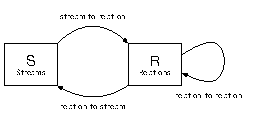
\includegraphics[width=.65\textwidth]{img/cql-model}\\
    \caption{The CQL processing model.}
    \label{fig:cql-model}
  \end{center}
\end{figure}

Figure~\ref{fig:cql-model} depicts the three operators defined by the CQL processing model. 
\begin{itemize}
\item[(i)] The stream-to-relation. It takes a stream S as input and produces a relation R as output, maintaining the schema. At any instant~$\tau$, $R(\tau)$ should be computable from S.
\item[(ii)] The relation-to-relation operator. It takes one or more relations $R_1,... , R_n$ as input and produces a relation R as output. At any instant $\tau$, $R(\tau)$ should be computable from $R_1(\tau),... , R_n(\tau)$.
\item[(iii)] The relation-to-stream operator. It takes a relation R as input and produces a stream S as output maintaining the schema. At any instant $\tau$, S at $\tau$ should be computable from R up to $\tau$.
\end{itemize}

CQL, also, define an abstract semantics for the data management:
\begin{Definition}
(Continuous semantics) Consider a query Q that is a composition of the three basic CQL operators. 
The inputs to the operators operators of Q are streams $S_1, ..., S_n (n \geq 1)$ and relations $R_1,..., R_m (m \geq 0)$. 
The result of continuous query Q at a time $\tau$ when all inputs are "available" can be defined as:
\begin{enumerate}
\item If the top operator in Q is relation-to-stream and produces the stream S, the result of Q at time $\tau$ is S up to $\tau$, produced by recursively applying the operators comprising Q to streams $S_1, ..., S_n$ up to $\tau$ and relations $R_1,..., R_m$ up to $\tau$.
\item If the top operator in Q is stream-to-relation or relation-to-relation and produces the relation R, the result of Q at time $\tau$ is $R(\tau)$, produced by recursively applying the operators comprising Q to streams $S_1, ..., S_n$ up to $\tau$ and relations $R_1,..., R_m$ up to $\tau$.
\end{enumerate}
\end{Definition}

\paragraph{Stream-to-relation operators}
The stream-to-relation operators in CQL are based on the sliding window concept (see Section \ref{sec:rsp-ql}). CQL exploits the concepts of window to define three classes of sliding window: time-based, tuple-based and partitioned.

\begin{Definition}
(Window) A window $W(S)$ is a set of elements extracted from a stream S. 
\end{Definition}

Time-based sliding window operator's output is defined by sliding an interval of T time units over the stream $S$. 
\begin{Definition}
(Time-based sliding window) A time-based sliding window on a stream S takes a time-interval T as a parameter and is specified by following S in the query with [Range T].
The output relation R of S[Range T] is defined as:
\noindent\begin{align*}
R(\tau)=\{s \mid \langle s,\tau' \rangle \in S \wedge (\tau' \leq \tau) \wedge (\tau' \geq \max\{\tau - T,0\})\}
\end{align*}  
\end{Definition}

Tuple-based sliding window operator's output is defined by sliding a window of size N tuples over the stream $S$.
\begin{Definition}
(Tuple-based sliding window) A tuple-based sliding window takes a positive integer N as a parameter and is specified by following S in the query with [Rows N].
The relation R of S[Rows N], R($\tau$), consists of tuples obtained from the N elements with the largest timestamps in S no greater than $\tau$.
\end{Definition}

Partitioned sliding window logically partitions $S$ into different sub-streams based on equality of attributes $A_1, ..., A_k$, computes a tuple-based sliding window of size $N$ on each sub-stream, then the output relation is the union of these sub-windows.
\begin{Definition}
(Partitioned sliding window) A partitioned sliding window on a stream S takes a positive integer N and a subset $\{A_1, ..., A_k\}$ of S attributes as parameters. It is specified by following S in the query with [Partition By $A_1, ..., A_k$ Rows N].
Formally, a tuple s with values $a_1, ..., a_k$ for attributes $A_1, ..., A_k$ occurs in output instantaneous relation R($\tau)$ iff exists an element $\langle s,\tau' \rangle \in S$ such that $\tau' \leq \tau$ is among the N largest timestamps among elements whose tuples have values $a_1, ..., a_k$ for attributes $A_1, ..., A_k$
\end{Definition}

\paragraph{Relation-to-relation operators}
The relation-to-relation operators operators transform relations in other relations. 
They are often derived from typical relational queries, by applying the semantic mapping to time-varying relations.
Relational algebraic expressions are a well-known cases of this class of operators.

\paragraph{Relation-to-stream operators}
Starting from the concepts of stream and relation, CQL defines three classes of relation-to-stream operators: Istream, Dstream, and Rstream. 

\begin{Definition}
(Istream) The insert stream applied to relation R contains an element $\langle s,\tau \rangle$ iff the tuple s is in $R(\tau) - R(\tau - 1)$: 
\noindent\begin{align*}
Istream(R) = \bigcup_{\tau \geq 0} ((R(\tau) - R(\tau - 1)) \times \{\tau\}).
\end{align*} 
\end{Definition}

\begin{Definition}
(Dstream) The delete stream applied to relation R contains an element $\langle s,\tau \rangle$ iff the tuple s is in $R(\tau - 1) - R(\tau)$: 
\noindent\begin{align*}
Dstream(R) = \bigcup_{\tau \geq 0} ((R(\tau - 1) - R(\tau)) \times \{\tau\}).
\end{align*} 
\end{Definition}

\begin{Definition}
(Rstream) The relation stream applied to relation R contains an element $\langle s,\tau \rangle$ iff the tuple s is in $R$ at time $\tau$: 
\noindent\begin{align*}
Rstream(R) = \bigcup_{\tau \geq 0} (R(\tau) \times \{\tau\}).
\end{align*} 
\end{Definition}

The concepts introduced by CQL represent a fundamental theoretical base for the development of the stream processors, see Section~\ref{sec:vel-var-solutions}. We exploited these constructs during the development of our Streaming Computational Model, see Chapter~\ref{ch:computational}.  

\subsubsection{SECRET}\label{sec:secret}
In 2000s, different systems try to implement a streaming processing model (see Section~\ref{sec:vel-var-solutions}). Despite they are based on common concepts, they present significant differences in the way they manage data and queries.
In order to explain the differences in the behavior of window operators in the existing stream processing engines, Botan et el. present SECRET~\cite{DBLP:journals/pvldb/BotanDDHMT10}.
Differently from CQL, it assigns two time instants to each stream item: (i) the application and (ii) the system time. The former, already defined by CQL processing model, refers to the instant related to the event represented by the element in the stream. It is not unique (contemporaneity is allowed) and defines a partial order among the stream elements. The latter must be unique and introduces a total order in the stream. From a conceptual point of view, the application time represents the most relevant information, but the system time is also important to understand the correct behavior of the stream engine.

\begin{figure}[h]
  \begin{center}
    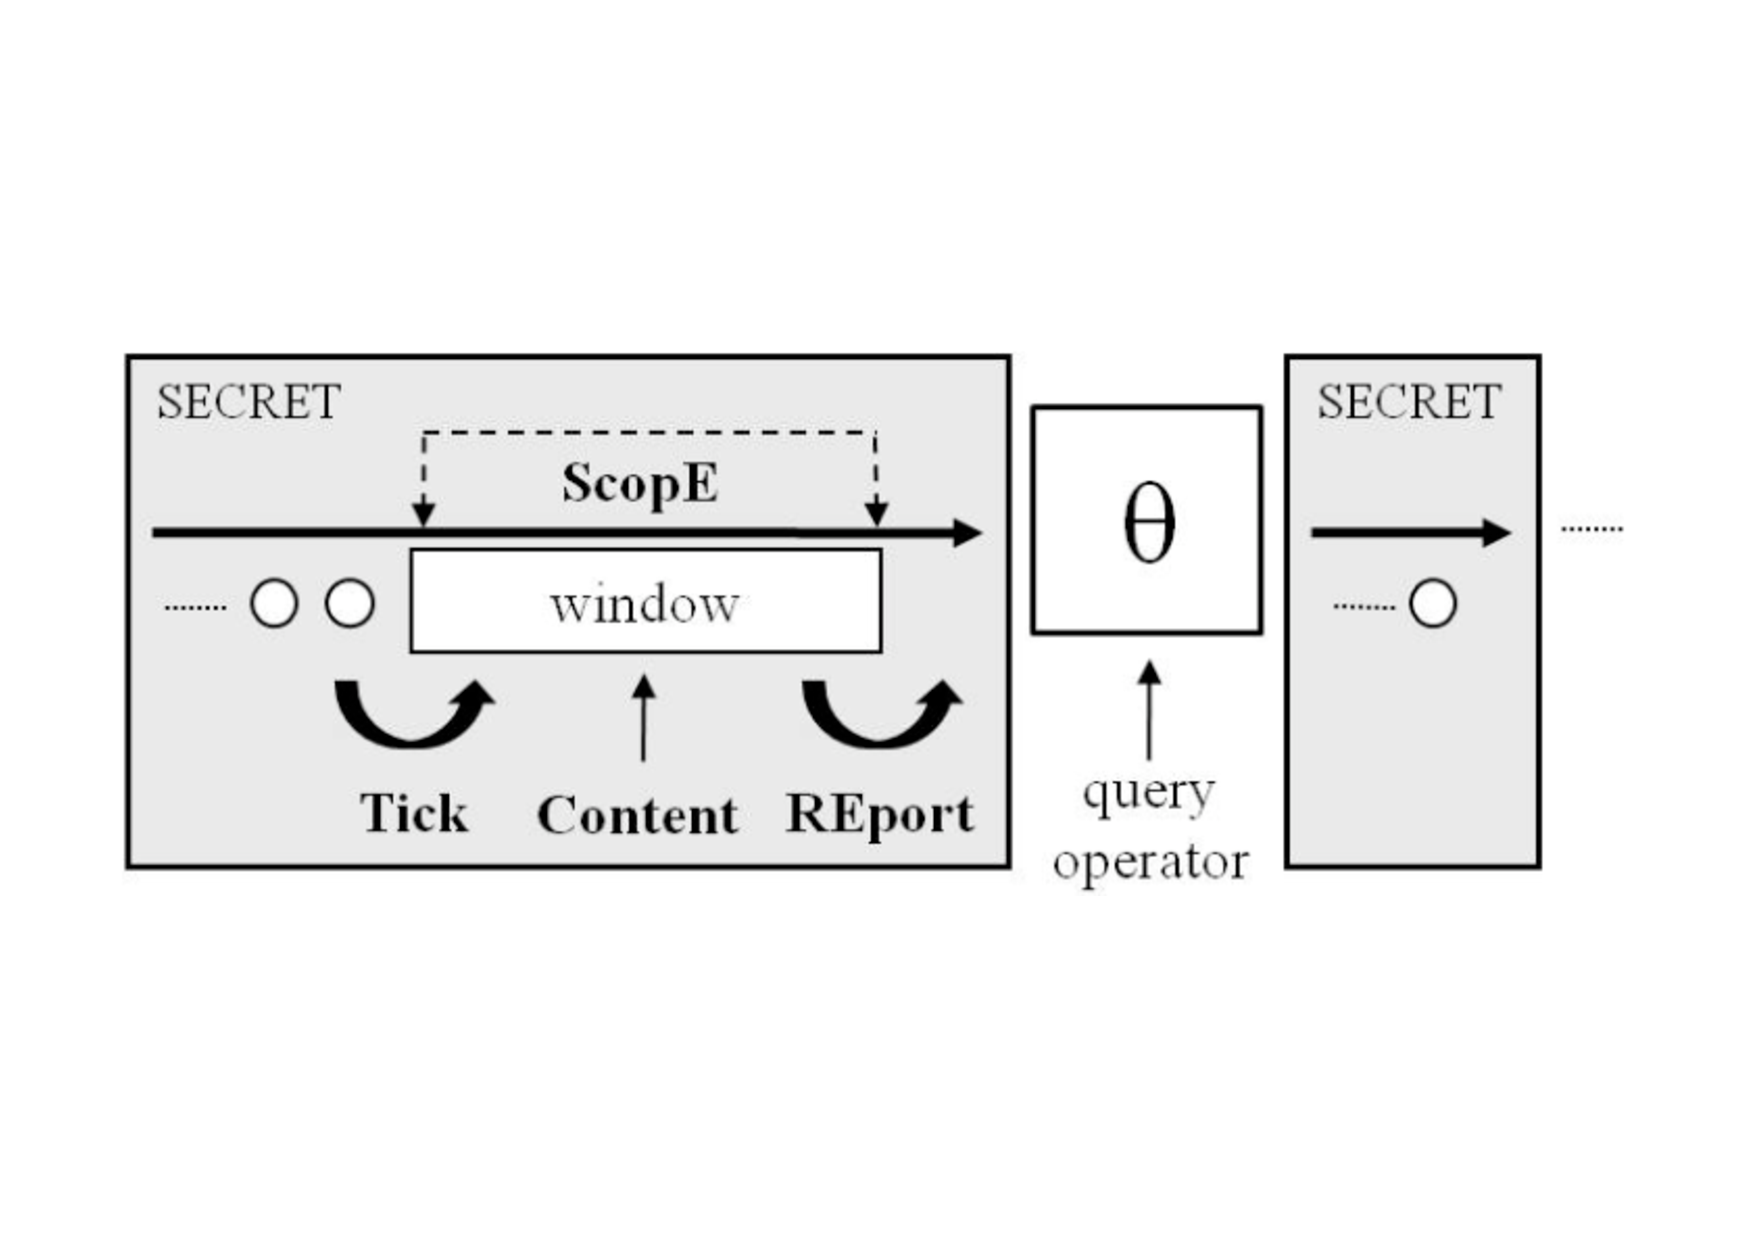
\includegraphics[width=0.8\textwidth]{img/secret}\\
    \caption{SECRET of a query plan (source \cite{DBLP:journals/pvldb/BotanDDHMT10}).}
    \label{fig:secret}
  \end{center}
\end{figure}

As depicted in Figure~\ref{fig:secret}, the SECRET framework introduces the notions of scope, content, report and tick to explain the window operator.

The \textit{Scope} function associates an evaluation time instant $t$ to the active window time interval. The computation of the scope relies on the $t_0$ parameter, the first active window start timestamp.

The \textit{Content} identifies the set of items of S in the active window. This function is influenced by both the application and the system time.

The \textit{Report} function defines the conditions under which the relation-to-relation operators can access the window content for additional query evaluation and result reporting. SECRET identifies four reporting strategies: (i) Content change -- the system reports if the content changes --, (ii)  Window close -- the system reports if the active window closes --, (iii) Non-empty content -- the system reports if the active window is not empty -- and, finally, (iv) Periodic -- the system reports only at regular intervals.

The \textit{Tick} is a function that defines under which conditions input can enter the window and, consequently, can be processed by the engine. SECRET defines tuple-driven and time-driven strategies. Systems that adopt the former strategy add the tuple to the window operator as soon as they arrive, contrariwise, systems that adopt the latter strategy, add tuple to the window at each application time instant.

The key concepts formalized by SECRETS result useful to guarantee a comparable behavior of all the different implementations of our Conceptual Model presented in Chapter~\ref{ch:computational}.

\subsection{Information Flow Processing and Architectures}\label{sec:vel-arch}
% This section introduces the information flow processing (IFP)~\cite{DBLP:journals/csur/CugolaM12}, an application domain in which, data from multiple distributed sources, needs to be processed in order to extract knowledge as soon as the relevant information is collected.
% In particular, we limit the overview to the IFP functional model (presented in the Section~\ref{sec:ifp-fm}), because it can be considered the foundation of the $\kappa$ architecture (see Section~\ref{sec:k-arch}) and $\lambda$ architecture (see Section~\ref{sec:l-arch}), that describe, from an higher point of view, the organization of a data processing architecture including stream processing components. 

Cugola et al. in~\cite{DBLP:journals/csur/CugolaM12} proposed the Information Flow Processing (IFP) as an application domain in which users need to collect information produced by multiple, distributed sources for processing it in a timely way in order to extract new knowledge as soon as the relevant information is collected.

From an high-level point of view, an IFP takes data flows from multiple sources as input, processes them and produces other information flows as output. This output is then directed toward a set of sinks.

\begin{figure}[h]
  \begin{center}
    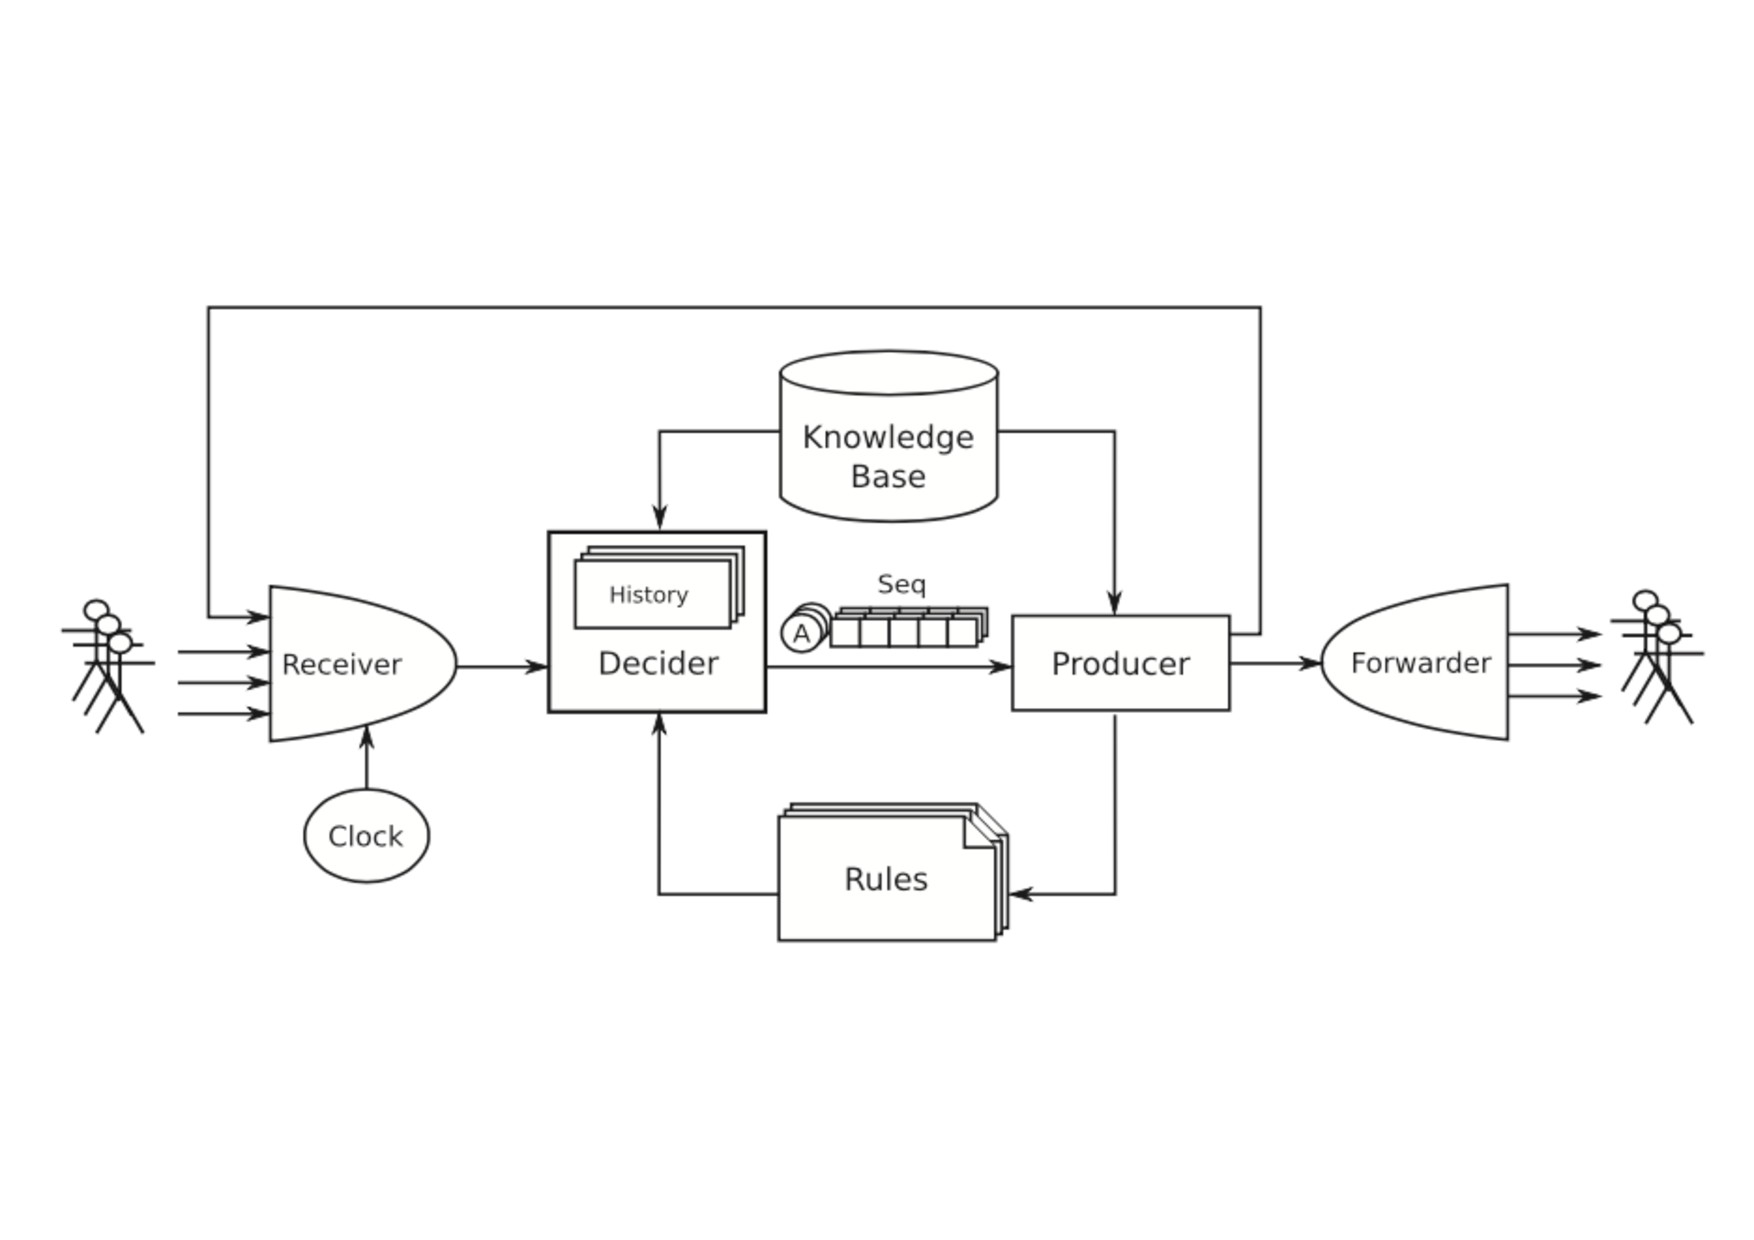
\includegraphics[width=\textwidth]{img/ifp}
    \caption{The functional architecture of an IFP system (source \cite{DBLP:journals/csur/CugolaM12}).}
    \label{fig:ifp}
  \end{center}
\end{figure}

Figure~\ref{fig:ifp} shows the components of a generic IFP system.
The \textit{receiver} implements the transport protocol to move data over the network and manages the connection between the sources and the IFP engine. Moreover, it is also connected to the \textit{clock} -- an architectural element that produces special data items that hold the current time.
Then, the data items, from external sources or from the clock, enter the processing pipeline that elaborates the data according to the rules stored into the rule store.
A rule is logically composed by a condition part (C) and an action part (A). C specifies the condition that has to be satisfied by the information to trigger the rule in the IFP, while A specifies what to do. The logical disjunction produces a physical disjunction, the processing are splitted in two different phases: (i) the detection -- realized by the \textit{decider} that checks the condition (C) on each incoming item --, and (ii) the production -- realized by the \textit{producer} that triggers the actions (A).
The \textit{knowledge base} represents a read only-memory\footnote{The knowledge base is read-only from the IFP engine perspective, but can be modified by external systems} that contains useful information for the decider and the producer.
Finally, the \textit{forwarder} is in charge to deliver the information to the output sinks.

In the early 2010s, Nathan Marz coined the term $\lambda$ architecture describing a generic, scalable and fault-tolerant data processing architecture that was very successful in distributed environment. 
The IFP functional model are at the basis of this architecture, formalizes by Marz et al. in ~\cite{marz2015big}.

\begin{figure}[t]
  \begin{center}
    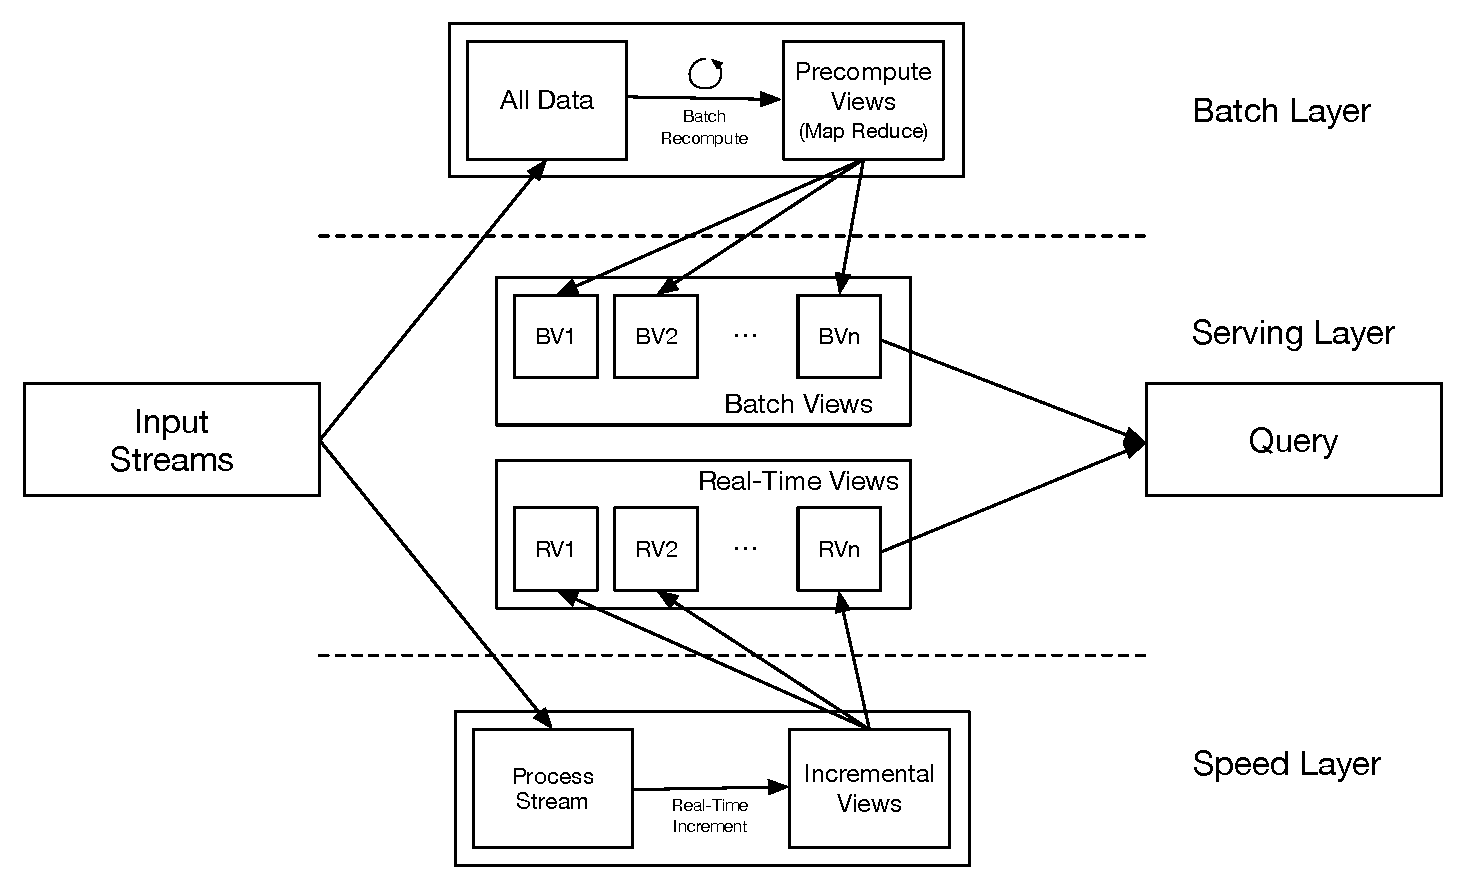
\includegraphics[width=\textwidth]{img/lambda-arch}
    \caption{The $\lambda$ architecture.}
    \label{fig:lambda-arch}
  \end{center}
\end{figure}

In a system implementing a $\lambda$ architecture (see Figure~\ref{fig:lambda-arch}), a separation between the batch processing pipeline (a.k.a. Batch Layer) and the real-time processing pipeline (a.k.a. Real-time Layer) is easily identifiable. This clear separation helps to isolate and localize the complexity of data update. The Serving Layer offers a mechanism to combine Batch Layer results with Real-time Layer results in order to offer the latest information to the user. The three layers are depicted in Figure~\ref{fig:lambda-arch}.
The Batch Layer is in charge of storing the immutable, constantly growing master dataset and of computing views from the stored dataset. 
The computation of the views is a periodic operation, the new data is aggregated once arrived and the views are incrementally computed on the entire dataset every time.
The Batch Layer operations could take hours to be completed, depending on the size of the cluster and of the data.
The Speed Layer compensates the high latency of the Batch Layer. It, normally, computes real-time views on the most fresh data. The views, computed by the Speed Layer, contain only the delta results to supplement the ones computed by the Batch Layer.
The Speed Layer continuously computes real-time views. That views are transient, once the information propagates through the Batch and Serving Layers the corresponding results in the real-time views lost its validity.
The Serving Layer is responsible for merging, indexing and exposing the views in order to make them available for query operations.

In recent years the complexity and the maintenance cost of $\lambda$ architectures were criticized\footnote{\url{https://www.oreilly.com/ideas/questioning-the-lambda-architecture}} and Jay Kreps proposed the $\kappa$ architecture\footnote{\url{http://milinda.pathirage.org/kappa-architecture.com/}}, a stream-only architecture.

\begin{figure}[t]
  \begin{center}
    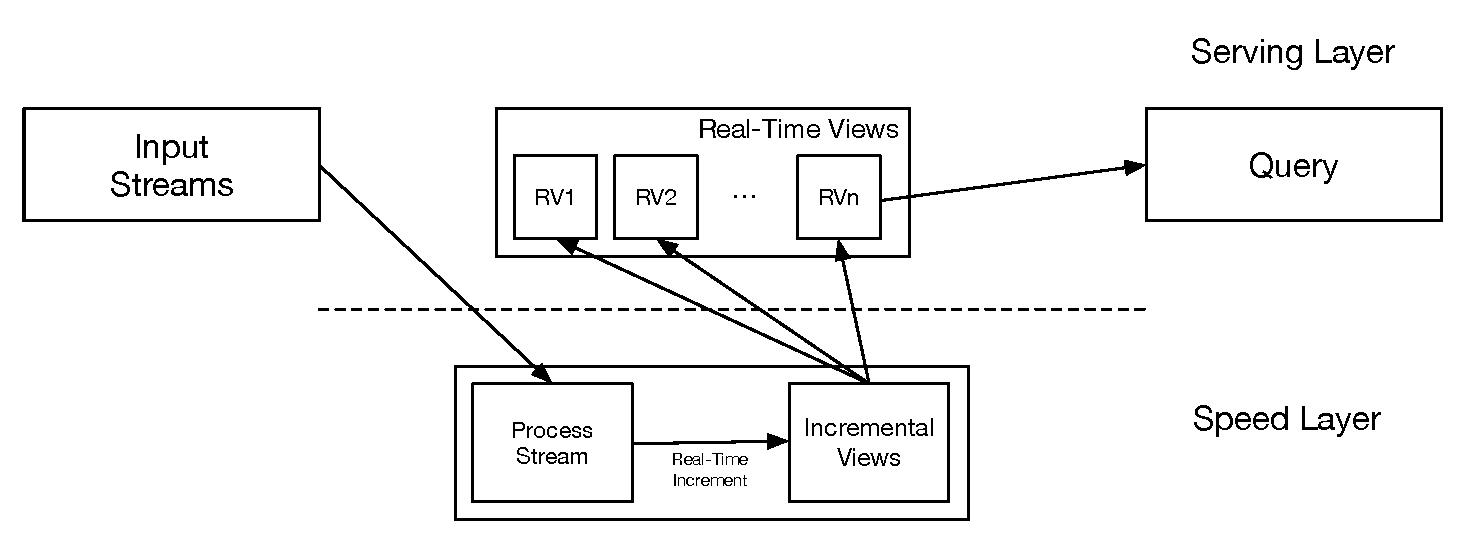
\includegraphics[width=\textwidth]{img/kappa-arch}
    \caption{The $\kappa$ architecture}
    \label{fig:kappa-arch}
  \end{center}
\end{figure}

Figure~\ref{fig:kappa-arch} depicts the main components of the $\kappa$ architecture, that aims at exploiting a single stream processing engine to handle real-time data processing and continuous reprocessing.
In this architecture the Speed Layer are in charge of computing real-time views on the most fresh data from the Input streams. The Real-Time views are incrementally computed when new data enters the system.
The most recent views are available to the Serving Layer for querying operation.
In a system based on a $\kappa$ architecture, the canonical data store is an append-only immutable log.

Both $\kappa$ and $\lambda$ architectures inspired our system presented in Section~\ref{sec:vel-sol} and our Computational Model presented in Chapter~\ref{ch:computational}.

\subsection{Open Source Solutions} \label{sec:vel-sol}
In this section, we present open-source solutions for taming velocity. All the proposed systems represent implementations of a $\lambda$ or a $\kappa$ Architecture. 
We choose to work with open-source software in order to explore and modify the internals to cope with our needs.
The section proposes one vertical scalable system (ESPER) and four different horizontally scalable systems with different characteristics (Kafka, Spark, Hive and Flink).
The proposed solutions inspired our streaming Computational Model proposed in the Chapter~\ref{ch:computational}.

\subsubsection{ESPER \& EPL} \label{sec:esper-epl}
Esper\footnote{\url{http://www.espertech.com/esper/}} is an open-source system for complex event processing (CEP) and streaming analytics. 
Esper exploits in-memory processing to address the requirements of applications that analyze high volume of fast data (between 1,000 to 100k messages per second in input), and must promptly react to events (from a few milliseconds to a few seconds of latency) by applying complex computations (e.g., pattern detection, filter, aggregation, etc.)

The Event Processing Language (EPL) offers SELECT, FROM, WHERE, GROUP BY, HAVING and ORDER BY clauses and is compliant to the SQL-92 standard.
In the EPL logic, streams replace tables as primary source of data and, instead of rows, events become the basic information unit. As for rows in the relational environment, events are composed by data.
EPL allows the definition of windows over stream of data to define a subset of the data to be analyzed. Such windows can be time-based or event-based (see Section~\ref{sec:CQL}) and can be combined applying intersection or union operators. Moreover, EPL provides the concept of named window, a data windows that can be used in multiple statements via the FROM clause, in a join or in a sub-query. 

Together, Esper and EPL, provide a powerful and extendable environment for stream processing and implements the basic concepts of a $\kappa$ Architecture (see Section~\ref{sec:vel-arch}).
Esper is a key components of the C-SPARQL Engine (see Section~\ref{sec:vel-var-solutions}).

\subsubsection{Apache Kafka \& KSQL} \label{sec:kafka}
Apache Kafka \cite{kreps2011kafka} is a distributed message broker with stream processing capabilities. Kafka organizes data into \textit{topics}. Each topic is made up of one or several \textit{partitions}. Each partition is assigned to a node in the Kafka cluster. 

The Kafka APIs are based on the \textit{producer} and \textit{consumer} components. The producer is responsible for transferring data from an external source to a Kafka cluster. Conversely, the consumer is responsible for reading data from a Kafka cluster and sending it to an external sink. By instantiating and using these components, an application can integrate Kafka as its storage solution. Kafka is designed to enable high-throughput applications, and it supports at-least-, at-most-, and exactly-once message delivery.

KSQL\footnote{\url{https://www.confluent.io/product/ksql/}} is a streaming SQL engine for real-time data processing against Apache Kafka. KSQL offers SQL-like language and ensures scalability and fault-tolerancy while enabling commons streaming operations (e.g. window, filter, aggregations, etc).

A system based on Kafka and KSQL enables all the commons operators described in CQL (see Section~\ref{sec:CQL}) and represents an implementation of a $\lambda$~Architecture (see Section~\ref{sec:vel-arch}).
Kafka is a key component of the infrastructure we used to test our work, see Section~\ref{sec:comp-mod-eval-cost}

\subsubsection{Apache Spark} \label{sec:spark}
Apache Spark \cite{zaharia2016apache} is a distributed processing engine which improves the Apache Hadoop~\cite{dean2008mapreduce} cluster computing paradigm for processing massive amounts of data in parallel. The main advantage over Apache Hadoop is that intermediate results can be stored into main memory, thus reducing disk I/O operations.

Spark environment consists of several components, which communicate with each other via the network. The highest level components are the \textit{master} and the \textit{workers}. The master is responsible for coordinating the execution of a Spark application and presenting its results. The workers are responsible for managing the execution of the distributed application code. There can be more than one worker, and each physical machine can host several workers. Both the master and the workers are implemented as separate processes running in the JVM.

Apache Spark is based on the Resilient Distributed Dataset (RDD) abstraction. An RDD represents an immutable dataset distributed over a cluster of machines. Each fragment of the dataset is termed a \textit{partition}. A Spark application consists of a sequence of transformations on a collection of RDDs. During execution, these transformations run in parallel on each partition. When an aggregated result is needed, e.g. COUNT after GROUP BY, Spark performs a shuffle operation by transferring partitions over the network between workers. Each worker spawns several subprocesses known as \textit{executors}. Executors run the distributed application code. The atomic unit of parallel execution is called a \textit{task}. At runtime each task is assigned to an executor.

Spark Streaming~\cite{DBLP:conf/sosp/ZahariaDLHSS13} is an extension of the core Spark API that enables scalable, high-throughput, fault-tolerant and real-time processing of data. 
It offers adapters for various data sources (e.g. Kafka, Flume, etc.).
The key abstraction behind Spark Streaming is the DStream (Discretized Stream), a potentially infinite flow of small batches. DStream are built on RDDs.
Spark Streaming represents an attempt to enable streaming, interactive, and batch queries in a single engine that supports: (i) continuous aggregations, (ii) windowing operations, (iii) stateful stream aggregations, and (iv) stream watermark operations.

Structured Streaming~\cite{DBLP:conf/sigmod/ArmbrustDTYZX0S18} is a new declarative streaming API available starting from Apache Spark 2.0 to support continuous applications. It is a higher-level API than the one offered by Spark Streaming and it is integrated into Dataset and DataFrame API.
Structured Streaming treats all the input data as an unbounded input table, each new items is appended once arrived. The queries see the input as a static table and the system compute the results incrementally.
Structured Streaming represents streams as DataFrames or Datasets with the isStreaming property set to true, therefore, the creation of an application with both stream and batch operations results very simple. A developer has just to describe the query at higher level, with few information about input, output and other details, and the system runs the query incrementally supporting consistency and recovery operations.

We exploited Spark Structured Streaming to create a distributed implementation of our streaming Computational Model presented in the Chapter~\ref{ch:computational}.

\subsubsection{Apache Hive} \label{sec:hive}
Apache Hive~\cite{DBLP:journals/pvldb/ThusooSJSCALWM09} is an open-source data ware-housing solution built on top of Apache Hadoop~\cite{dean2008mapreduce}. It offers a SQL-like declarative language, namely HiveQL, that supports the insertion of custom map-reduce scripts directly into queries.

Hive data is organized into: (i) the Database -- the counterpart of the relational databases --, (ii) the Table -- an abstraction of the classic relational tables, it corresponds to an HDFS directory that contains the serialized data --, (iii) the Partition -- it represents the organization of the data in the sub-directories tree --, (iv) the Bucket -- a division of the data within a partition, a single bucket is represented as a single file.
Hive has a limited support to streaming data. Hive Streaming API allows a system to continuously ingest information in small batches into an existing Hive partition or table. Once the flowing information is committed, it becomes immediately available to all Hive queries.

HiveQL supports primitive data-types within a table, but the underlying IO libraries can be extended to access data in custom formats.
Hive includes a system catalog, the Hive-Metastore. It contains schemas and statistics to be used during the data exploration phases.
HiveQL support a simple window operator\footnote{\url{https://cwiki.apache.org/confluence/display/Hive/LanguageManual+WindowingAndAnalytics}} that can partially simulate the CQL window operator (see Section~\ref{sec:CQL}).  

Hive implements typical batch operator and offers a minimal support for the streaming operations (i.e. window operator). We exploited Hive windows to implement a distributed version of Our streaming Computational Model presented in the Chapter~\ref{ch:computational}.

\subsubsection{Apache Flink}
Apache Flink \cite{DBLP:journals/debu/CarboneKEMHT15} is a distributed platform for streaming data (DataStream API) and batch data (DataSet API). The dataflow engine, the core of the platform, guarantees the fault tolerance during the distributed computations.
Flink's provides an event-at-a-time processing model throw a dataflow of streams and transformations. The DataStream API enables classic stream processing operations (e.g., filters, aggregations, window functions) on bounded or unbounded streams of data, the DataSet API enables transformations (e.g. filters, mapping, joining, grouping) only on finite dataset.

Flink offers a relational abstraction of the data, the Table, that can be created from external data sources or from existing DataStreams and DataSets. The table can be accessed via: (i) the Tables API, a SQL-like expression language that supports relational operators (e.g., selection, aggregation, joins); and via (ii) regular SQL. Both of the access methods offer equivalent functionalities and can be mixed in the programming flow.

Flink can natively manage both stream and batch of data. A system based on it, represents an implementation of a $\lambda$ architecture (see Section~\ref{sec:vel-sol}).

\section{Variety}\label{sec:variety}
In the next sections, we present an overview of the Models, Languages and Methodologies to tame the data variety. After an overview on the main concepts behind RDF, SPARQL and R2RML mapping language, we go through the ontological world.
Gruber in \cite{DBLP:journals/ijmms/Gruber95} define an ontology as "an explicit specification of a conceptualization". A conceptualization is defined as "the objects, the concepts and other entities that are assumed to exist in some area of interest and relationships that hole among them" ~\cite{DBLP:books/daglib/0005829}. An ontology, with its capability to offer a common representation of heterogeneous data, offers a good starting point in facing the variety problem.
The following sections present OWL, an overview of two ontology engineer methodologies (METHONTOLOGY and NEON) and OBDI as an example of integration methods based on ontologies.   
Finally, we present the open source solutions that we exploited during our research work.

\subsection{Models, Languages and Methodologies}

\subsubsection{RDF \& SPARQL}\label{sec:rdf-sparql}
The Resource Description Framework (RDF) is a W3C standard for data interchange on the Web~\cite{cyganiak2014rdf}. 
The main data structure in RDF is the directed labeled graph, made of nodes, which represent the resources and of edges which represent the relations between them. The atomic RDF element is the triple that consists of subject, predicate, and object. We identify with I, B and L respectively the sets of IRIs, blank nodes, and literals. We define an RDF term as an element of the set $I \cup B \cup L$.

\begin{Definition}
(RDF statement and RDF graph). An RDF statement is a triple $(s, p, o) \in (I \cup B) \times (I) \times (I \cup B \cup L)$, while a set of RDF statements is called an RDF graph, which is a directed, labeled graph that represents Web resources.
\end{Definition}

The SPARQL Protocol and RDF Query Language (SPARQL)~\cite{harris2013sparql} is W3C Recommendation and enables data retrieve, data manipulation and query operation on data stored in RDF format.
A SPARQL query typically contains one or more triple patterns called a basic graph pattern, it is similar to an RDF triple except for the possible presence of variables instead of resources.

\begin{Definition}
(Triple pattern and Basic Graph Pattern). A triple pattern $tp$ is a triple $(sp, pp, op)$ such that
\noindent\begin{align*}
(sp, pp, op) \in (I \cup B \cup V ) \times (I \cup V ) \times (I \cup B \cup L\cup V ),
\end{align*}  
where $V$ is the infinite set of variables. 
A basic graph pattern is a set of triple patterns.
Graph patterns in a SPARQL query can include basic graph patterns and other compound expressions defined recursively as:
\begin{enumerate}[nosep]
\item A set of triple patterns is a basic graph pattern;
\item If $P_1$ and $P_2$ are graph patterns, then ($P_1$ AND $P_2$), ($P_1$ OPT $P_2$) and ($P_1$ UNION $P_2$) are graph patterns;
\item If $P$ is a graph pattern and u is a symbol in $I \cup V$, (GRAPH $u$ $P$) and (SERVICE $u$ $P$ ) are graph patterns;
\item If $P$ is a graph pattern and $R$ is a SPARQL built-in condition, then ($P$ FILTER $R$) is a graph pattern.
\end{enumerate}
\end{Definition}

A SPARQL built-in condition consists of the elements of the set
$(I\cup L \cup V)$ and constants, logical connectives $(\neg, \vee, \wedge)$, the binary equality symbol $(=)$, ordering symbols
$(<,\leq,\geq,>)$, and unary predicates such as $bound$,
$isBlank$, $isIRI$.

To introduce the evaluation semantics of a SPARQL query, we define solution mapping as detailed in~\cite{DBLP:journals/tods/PerezAG09,harris2013sparql}.

\begin{Definition}
(Solution mappings). A solution mapping $\mu$ is a partial function $\mu \colon V \rightarrow I \cup B \cup L$. It maps a set of variables to a set of RDF terms. 
A mapping has a domain $dom(\mu)$ which is the subset of V over which it is defined. We denote as $\mu(x)$ the RDF term resulting by applying the solution mapping to variable $x$. We denote as $\omega$ a multiset of solution mappings, and as $\psi$ a sequence of solution mappings. 
Typical relational algebraic operators can be applied to multiset of solution mappings:
\begin{itemize}[label={}, nosep]
\item $\Omega_1\Join\Omega_2 = \{\mu_1 \cup \mu_2 | \mu_1 \in \Omega_1 \wedge \mu_2 \in \Omega_2 \wedge \mu_1 \sim \mu_2\}$
\item $\Omega_1 \cup \Omega_2 = \{\mu| \mu_1 \in \Omega_1 \vee \mu_2 \in \Omega_2\}$
\item $\Omega_1 \backslash \Omega_2 = \{\mu| \mu \in \Omega_1 \wedge \nexists \mu_1 \in \Omega_2 \colon \mu \sim \mu_1\}$
\item $\Omega_1\leftouterjoin\Omega_2 = (\Omega_1\Join\Omega_2) \cup (\Omega_1 \backslash \Omega_2)$
\end{itemize}  
\end{Definition}

RDF datasets is a collections of one or more RDF graphs and represents the format of input data.
\begin{Definition}
(RDF dataset). An RDF dataset DS is a set: 
\noindent\begin{align*}
DS = {G0, (u1, G1), (u2, G2), ...(un, Gn)}
\end{align*}
where G0 and Gi are RDF graphs, and each corresponding ui is a distinct IRI. G0 is called the default graph, while the others are called named graphs. During the evaluation of a query, the graph from the dataset used for matching the graph pattern is called active graph. Multiple graphs can become active during the evaluation, but only one at time.
\end{Definition}

SPARQL defines four query forms: SELECT -- which produces a result of variable bindings matching the graph pattern --, CONSTRUCT, which produces a new RDF graph with the query solutions --, ASK -- which produces a boolean value that is true if at least a solution exists --, and DESCRIBE -- which produces an RDF description of resources in the solution.
A query can also contain solution modifiers (e.g., LIMIT, DISTINCT, ORDER BY) that are applied after pattern matching.
A SPARQL query \cite{DBLP:journals/tods/PerezAG09} can be defined as:

\begin{Definition}
(SPARQL Query). A SPARQL query is defined as a tuple (E, DS, QF), where E is a SPARQL algebraic expression, DS is an RDF dataset, and QF is a query form.
\end{Definition}

A query solution is a bag of solution mappings that assign RDF triples to variables of the query.
The evaluation semantics of a SPARQL query algebraic expression w.r.t. an RDF dataset is defined for every operator of the algebra, and it is expressed through an evaluation function.

\begin{Definition}
(SPARQL evaluation semantics). The SPARQL evaluation semantics of an algebraic expression E is denoted as ED(G), where DS(G) is the dataset DS with active graph G.
\end{Definition}

RDF and SPARQL represent a fundamental concepts in the data variety management, both in static and streaming environment (see Section~\ref{sec:vel-var}).

\subsubsection{R2RML}
The RDB to RDF mapping language\footnote{\url{http://www.w3.org/TR/r2rml/}} (R2RML) is a language to create custom mappings to transform relational data into RDF.
R2RML mappings file presents itself as an RDF graphs and, unlike Direct Mapping\footnote{\url{https://www.w3.org/TR/rdb-direct-mapping/}} (DM), allows user to define highly customized views over relational data sources. The R2RML conceptual mapping is tailored to a specific database schema and target vocabulary (i.e., the input database must conform to the presented schema) and produces an RDF dataset (see Section~\ref{sec:rdf-sparql}) that conforms to the target vocabulary. The R2RML processors can work as a virtual access layer to the relational data or can materialize the output data.

\begin{figure}[t]
  \begin{center}
    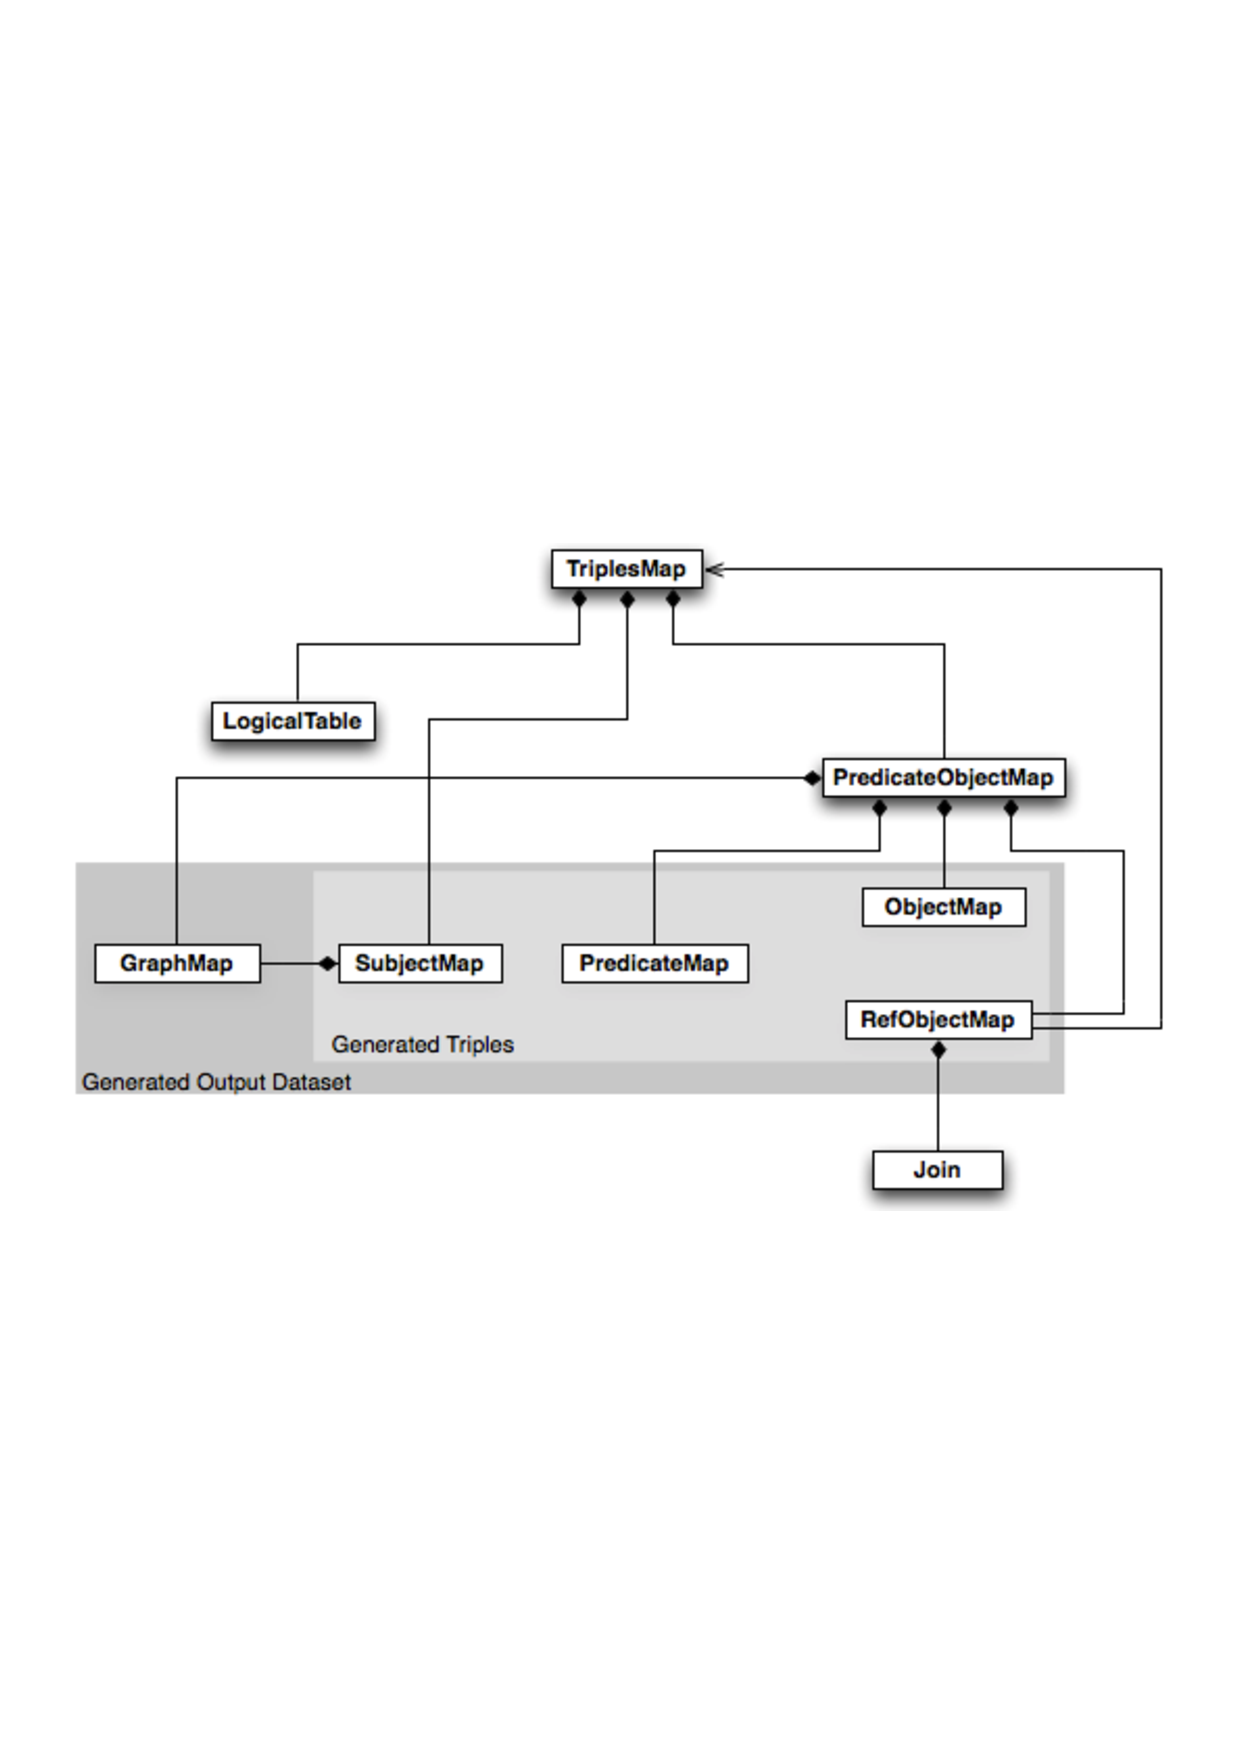
\includegraphics[width=0.8\textwidth]{img/R2RML}
    \caption{R2RML mapping process (source: https://www.w3.org/TR/r2rml).}
    \label{fig:r2rml}
  \end{center}
\end{figure}

Figure~\ref{fig:r2rml} depicts the overview of the mapping process.
R2RML mapping accesses to the relational input data through logical tables. A logical table can be a base table in the input database, a view or a valid SQL query (R2RML view).
Each logical table is then mapped to RDF using a triple map, a set of rules that allows the system to transform each row in the logical table into one or more RDF triples. The rules are composed by a subject map that creates the subject for all the triples generated by a single row and by multiple predicate-object maps that consist of predicate maps and object maps.

\subsubsection{OWL} \label{sec:owl}
The Web Ontology Language (OWL)\footnote{\url{https://www.w3.org/TR/owl-features/}} is a W3C Semantic Web language designed for creating ontologies.
OWL is part of the W3C's Semantic Web technology stack. It is a computational logic-based declarative language  characterized by formal semantics.
The knowledge expressed in OWL can be reasoned to verify the consistency of that knowledge or to make implicit knowledge explicit.
The fundamental notions exploited by OWL to represent knowledge are: (i) the Axioms -- the basic statement of an ontology --, (ii) the Entities -- the representation of a real world object --, and (iii) the Expressions -- a combination of entities to describe a complex object.

The three concepts presented above allow OWL to create a human-like knowledge representation with the concept of consequence. When a statement is a consequence of another statement, it is true whenever the other statements are. In OWL, a set of statements \textit{S} entails a statement \textit{s} if in any state of affairs wherein all statements from \textit{S} are true, also \textit{s} is true. A set of statements may be consistent (there is a possible state in which all the statements in the set are jointly true) or inconsistent (there is no such state). The formal semantics of OWL specifies for which condition a particular set of OWL statements is true.

The W3C-endorsed OWL specification includes the definition of three variants of OWL: OWL Lite, OWL DL and OWL Full, presented in order of expressiveness.
OWL2\footnote{\url{https://www.w3.org/TR/owl2-overview/}} represents the latest specification of the  Web Ontology Language. It is dated to 2009 and introduces three additional profiles: OWL2EL, a fragment with polynomial time reasoning complexity; OWL2QL, a language to enable easier access and query to data stored in databases; and OWL2RL, a rule subset of OWL2.

The Conceptual Model presented in the Chapter \ref{ch:conceptual} is formalized with OWL2.

\subsubsection{Ontology Engineering}\label{sec:onto-eng}
We report a briefly overview of METHONTOLOGY, an ontology development methodology we exploited in the definition of the Conceptual Model presented in Chapter~\ref{ch:conceptual}, and NeOn, an evolution of METHONTOLOGY, that supports the reuse of already available ontologies.

\textbf{METHONTOLOGY}~\cite{fernandez1997methontology} is a methodology for creating ontologies from scratch, by reusing other ontologies or by re-engineering them. The framework enables the construction of ontologies at the "knowledge level". 

\begin{figure}[h]
  \begin{center}
    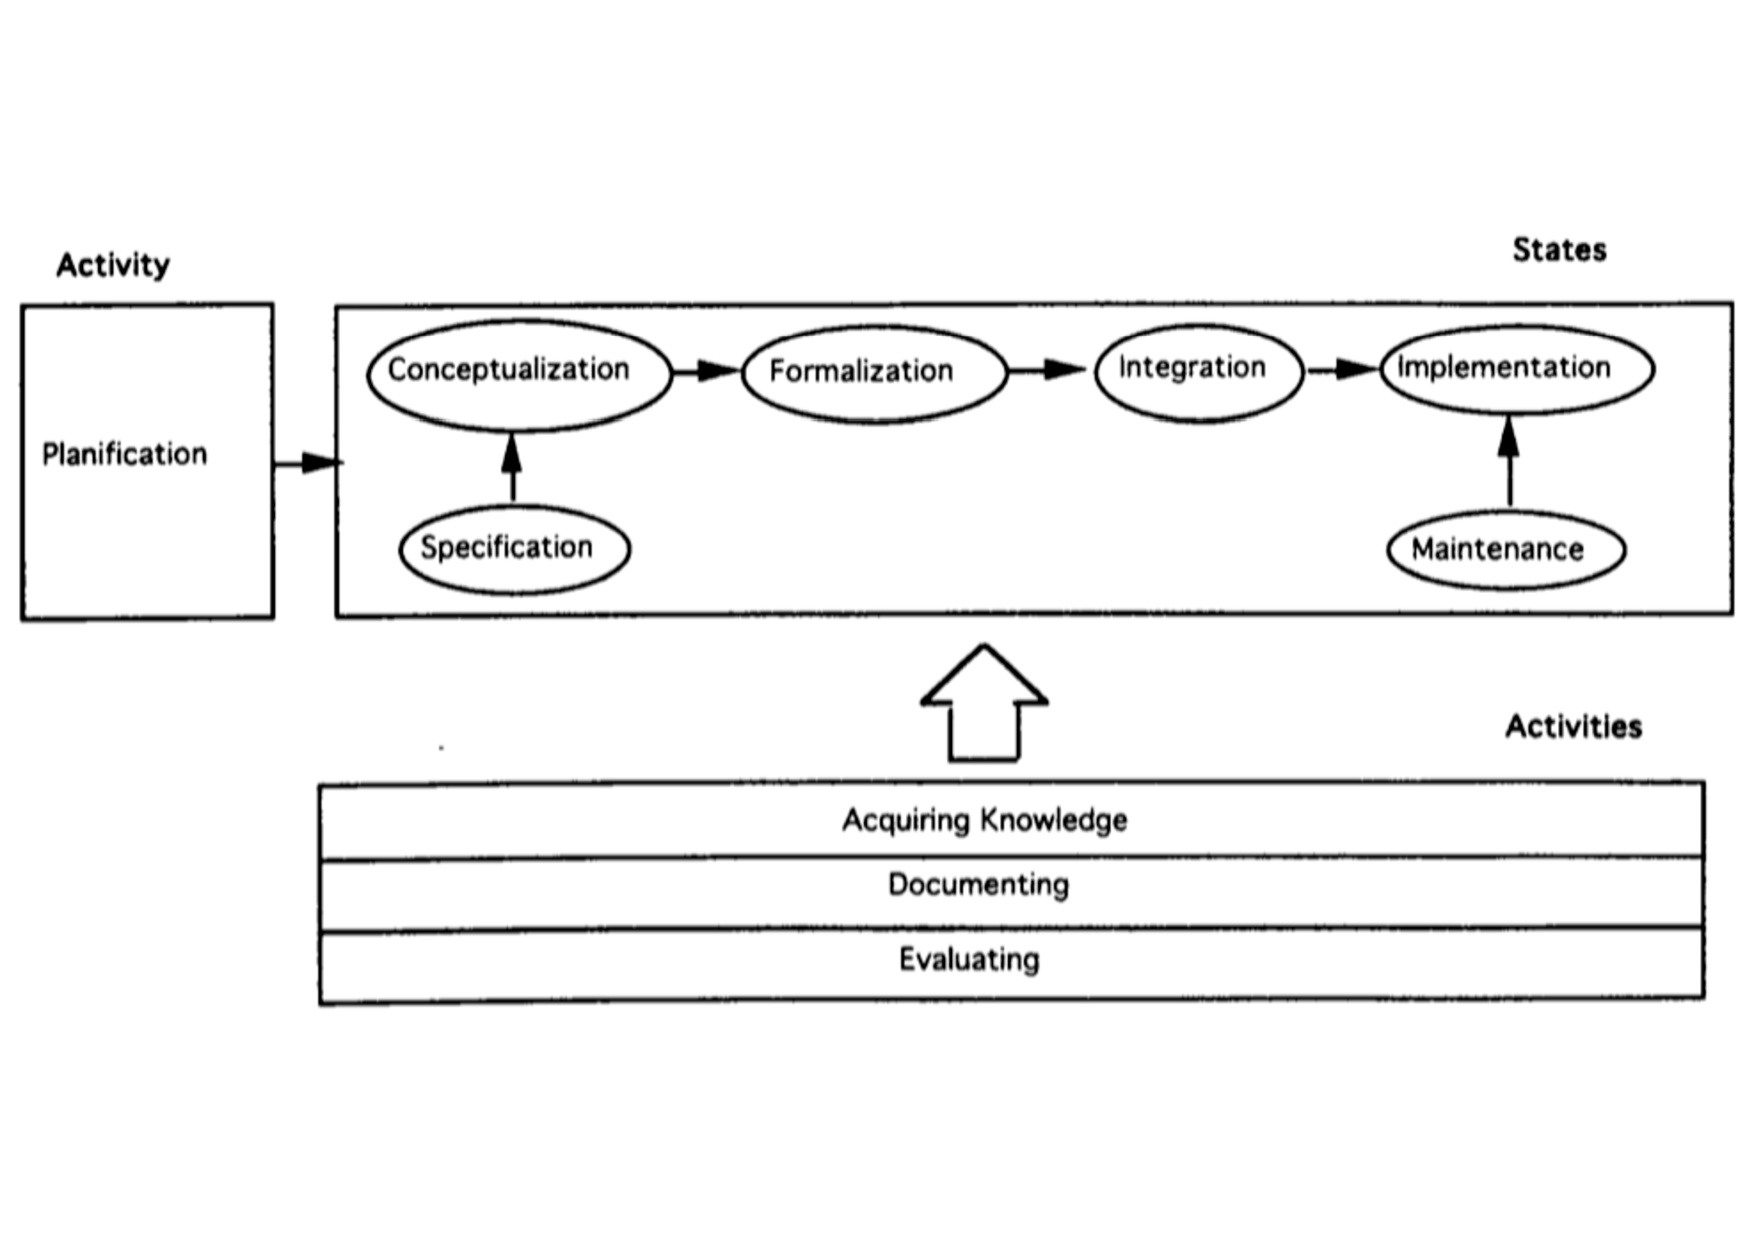
\includegraphics[width=0.8\textwidth]{img/methontology}
    \caption{Ontology lifecycle (source~\cite{fernandez1997methontology}).}
    \label{fig:methontology}
  \end{center}
\end{figure}

It includes: (i) the formal identification of the development process and its phases (i.e., scheduling, control, quality assurance, specification, knowledge acquisition, conceptualization, integration, formalization, implementation, evaluation, maintenance, documentation and configuration management); (ii) an evolving prototypes based lifecycle (see Figure~\ref{fig:methontology}) that identifies the phases the ontology passes during its lifetime and the interdependencies with the lifecycle of the connected ontologies; (iii) the specific techniques to perform each activity, the output of each phases and the evaluation methods.

The \textbf{NeOn}~\cite{DBLP:phd/dnb/Suarez-Figueroa12} methodology encourage the reuse of other ontologies as well as of non-ontological resources during the engineering process. The framework provides strong guidelines for the execution of the development activities (e.g., the usage of ontology design patterns). 

\subsubsection{OBDI \& OBDA}\label{sec:obdi-obda}
The data integration problem consists of combining data from heterogeneous sources, and offering the user a unified view of the information. Due to the growing number of data sources (e.g., smartphones, sensors, etc), the  problem of designing data integration systems are becoming more and more important in the real-world.
Moreover, companies are shifting from centralized and self-contained way to manage their data (i.e., a central database or a data warehouse) to a distributed, interactive and multi-source world where the information becomes the exchange good. The volume and the heterogeneity of the data are constantly growing and companies are now focusing on finding the right information.
Most of the available sources is characterized by syntactic, structural and semantic heterogeneities.

In a generic data integration system~\cite{LenzeriniOBDI}, the sources contain the real data, while a global schema offers an integrated and reconciled overview of such sources. Modeling the relation (namely, the mapping) between the sources and the global schema represents an important aspects of the data integration process.
The data integration issue have been faced following three different approaches: (i) the Global-As-View (GAV) approach -- the most used form of mappings, where the data schema is expressed in terms of the data sources --, (ii) the Local-As-View (LAV) approach -- where the data schema is specified independently from the sources --, and a hybrid approach (GLAV) -- the most general form of mapping.
Independently from the approach, in a data integration system, the query process requires a reformulation step where the query over the global schema is reformulated in terms of a set of queries over the sources.

In several domains, such as Enterprise Application Integration, in the Semantic Web and, in particular, in the data integration~\cite{LenzeriniOBDI}, ontologies are considered as the ideal formal tool to provide a common conceptualization of the domain, and Description Logics (DLs) are widely considered appropriate for expressing ontologies. DLs are also at the basis of the OWL Language (see Section~\ref{sec:owl}).

Consequently, an Ontology-Based Data Integration (OBDI) system consists of three main components: (i) an ontology -- the formal description of the considered domain --, (ii) a set of data sources -- the repositories where data are stored --, and (iii) the mapping -- a specification of the correspondences between the data and the ontology elements. Such system allows users to access the data using the ontology components as a predicates. 
Differently from the traditional data integration, OBDI system offers a semantically rich description of the relevant concepts in the domain of interest and of the relationships between such concepts, in addition to a separation between the conceptual level (presented to the client through the ontology),
and the logical/physical level of the information system (the one stored in the sources).

Intuitively, in the simplest technique for enabling query answering, the system first retrieves the concepts and the roles instances from the data sources through the mapping and then, exploiting the ontology axioms, it "expands" such a set of (stated and inferred) instances deriving and materializing all the logically entailed concepts and roles assertions. 
In this way, the queries can be evaluated on the complete set of instances. Unfortunately, the set of entailed instance assertions may be infinite and, consequently, such a techniques is not feasible. 

Since 2000s, Ontology-Based Data Access (OBDA)~\cite{DBLP:journals/jods/PoggiLCGLR08} has become a popular approach to enable users to access data sources through an ontology.
Moreover, a GAV approach based on a data model expressed in OWL 2 QL (based on the DL-Lite family of description logics), ensures the effectiveness of query answering operation with LOGSPACE complexity (more precisely, AC\textsuperscript{0}).

In a classic OBDA framework, query rewriting starts from the computation of the perfect rewriting in order to enable the query evaluation on the data sources. The creation of the rewriting can be modularized into a first phase of of query rewriting related to the ontology and in a second phase of query rewriting related to the mapping.

During our research work we exploited OBDI and OBDA techniques in many applications (see Chapter~\ref{ch:case-studies}) using our Conceptual Model presented in Chapter~\ref{ch:conceptual} as the ontology to mediate between the user queries and the data.

\subsection{Open Source Solutions} \label{sec:var-solutions}
In this section, we present the solutions we used over the years in our research work. As usual in this research, we have privileged open source solution in order to access and exploits the internals.

We start from Jena and Sesame, frameworks to manage RDF data and to build Semantic Web applications.
\textbf{Apache Jena}\footnote{\url{https://jena.apache.org/}} is written in Java.
The main data structure in Jena is the Model, an abstract representation of an RDF graph.
A model can be accessed and queried via SPARQL and its source can be external file, databases, URLs or a combination of them.
Jena offers different components to support the creation of application, it provides the TDB, an RDF database that supports SPARQL 1.1 query, and Fuseki, a database server that support the access via the standard SPARQL protocols\footnote{\url{http://www.w3.org/TR/sparql11-protocol/}}. Jena is a core component of the C-SPARQL Engine (see Section~\ref{sec:vel-var-solutions}).

\textbf{Sesame}~\cite{DBLP:conf/semweb/BroekstraKH02} is an open-source framework for storing, querying and analyzing RDF data. It also offers support for RDFS inferencing and querying.
Sesame implements an in-memory/on-disk triplestore and offers a Servlet packages to manage and access the stored data on a permanent server. 
Sesame supports concurrency control, export of RDF and RDFS information and a query engine for RQL, SPARQL and SeRQL.
In May 2016, Sesame officially forked into an Eclipse project called RDF4J\footnote{\url{http://rdf4j.org}} that provides functionality for efficient and scalable storage, querying, and reasoning with RDF data, and a vendor-neutral access API for RDF databases.

To explore the basic reasoning techniques we worked with Hermit and RDFox. 
\textbf{HermiT}~\cite{DBLP:conf/owled/ShearerMH08} is a Description Logic reasoner based on a "hypertableau" calculus techniques, an innovative and efficient reasoning algorithm. It also incorporates the "anywhere blocking" strategy, which limits the sizes of constructed models.
HermiT uses direct semantics and is conformant to all OWL 2 tests for direct semantics reasoners.
\textbf{RDFox}~\cite{DBLP:conf/semweb/NenovPMHWB15} is a main-memory, scalable, centralized datalog engine. It supports materialization-based parallel reasoning, SPARQL query answering and implements Backward/Forward algorithm proposed in~\cite{DBLP:conf/aaai/MotikNPH15a}.
The innovative intuition is the combination of backward and forward reasoning to limit the recomputation performed by the traditional DRed~\cite{DBLP:journals/jods/VolzSM05}.

As OBDA framework, we used \textbf{OnTop}~\cite{DBLP:journals/semweb/CalvaneseCKKLRR17}, an open-source Ontology-Based Data Access (OBDA) system that offers a solid theoretical base, a virtual OBDA approach implemented with query rewriting technique, its compliance to W3C recommendations and its support for all major relational databases.

\begin{figure}[t]
  \begin{center}
    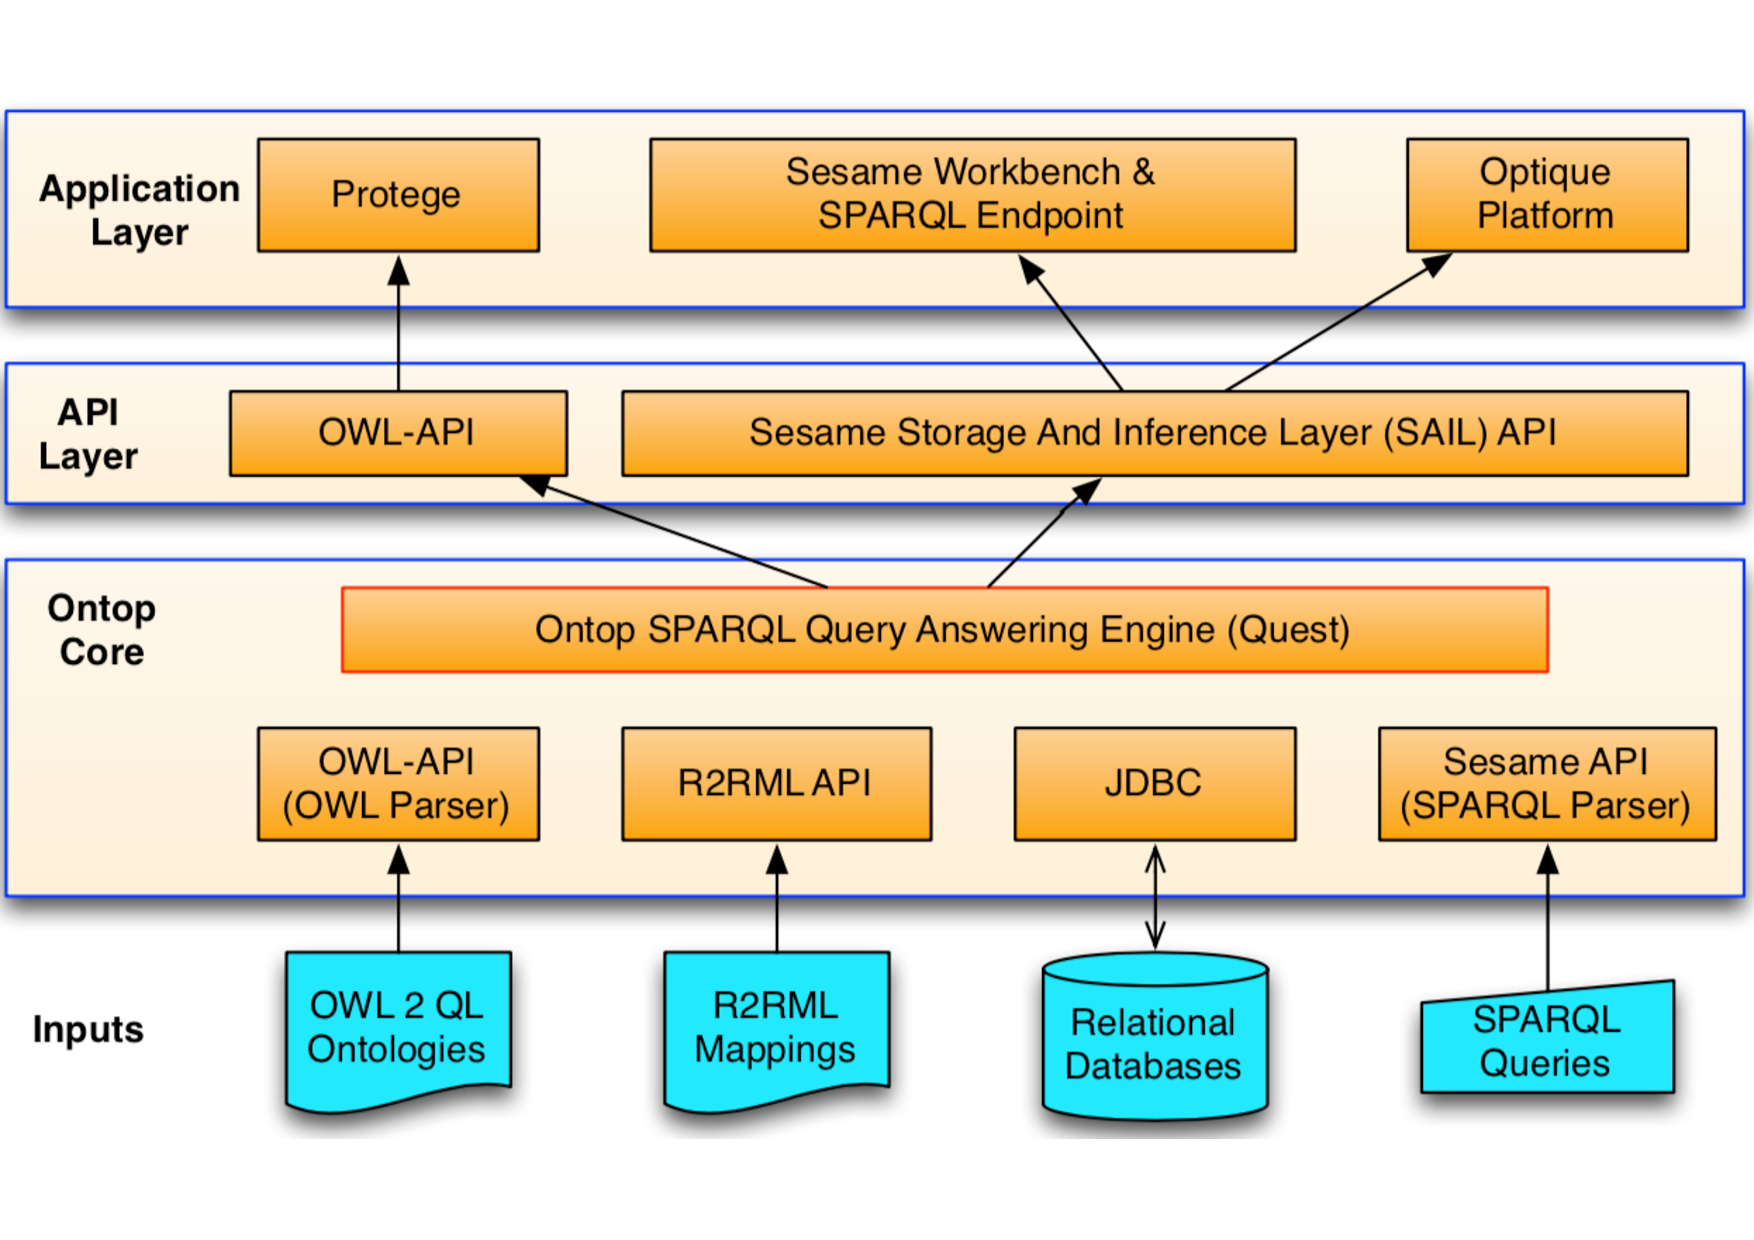
\includegraphics[width=0.8\textwidth]{img/ontop}\\
    \caption{Architecture of the Ontop system (Source \cite{DBLP:journals/semweb/CalvaneseCKKLRR17}).}
    \label{fig:ontop}
  \end{center}
\end{figure}

Figure \ref{fig:ontop} presents the four levels of a system based on Ontop: (i) the input, such as queries, database, ontology and mapping; (ii) the Ontop core needed to rewrite SPARQL queries SQL queries; (iii) the API for accessing system services; and (iv) the applications for the end-user to execute SPQARL queries over relational data.

\section{Velocity and Variety}\label{sec:vel-var}
In the next sections, we present the solution to manage the data variety in a streaming fashion. We start from the formal definition of the concepts behind Stream Reasoning and RDF Stream Processing (RSP). We present RSP-QL, an attempt to unify the different RSP query languages developed over the years by the RSP community and, finally, we present an overview of the currently available solutions.

\subsection{Models and Languages}
\subsubsection{Stream Reasoning \& RDF Stream Processing}\label{sec:sr-rsp}
In 2009, Della Valle et al. \cite{della2009s} proposed to start to investigate on how to represent, manage, and reason on heterogeneous continuously flowing data in the presence of expressive domain models.

In a scenario, where an ontology offers a conceptual view over autonomous data sources, a reasoner can play a key role in finding answers that are not syntactically present in the data sources, but are derivable from the data and the ontology (see Section~\ref{sec:obdi-obda} on OBDI and OBDA).
RDF (see Section~\ref{sec:rdf-sparql}) represent the dominant data model in the field of reasoning for data integration and RDF streaming languages (see Section~\ref{sec:vel-var-solutions}) bridge the gap between stream processing and OBDI. 
Reasoning in a streaming fashion looks conceptually simple, but it is hard to be efficiently performed. Della Valle et al. \cite{DBLP:conf/fis/ValleCBBC08} showed how continuous DL reasoning can be reduced to periodic repetition of reasoning over a windowed ontology stream.
Barbieri et al. \cite{DBLP:conf/esws/BarbieriBCVG10} presented an optimization of DRed algorithm when deletion becomes predictable. In parallel Komazec et al. \cite{DBLP:conf/debs/KomazecCF12} implemented an extension of the RETE algorithm, Ren at al. \cite{DBLP:conf/cikm/RenP11} approached the problem via truth maintenance systems and Motik et al. \cite{DBLP:conf/aaai/MotikNPH15a} represents the state of the art in this research field.
Still along this DL-centric line, more recently, Calbimonte et al. \cite{DBLP:conf/semweb/CalbimonteCG10} exploited OBDA principles by rewriting continuous ontological queries to a stream processing system. In parallel to this line, at the beginning of 2000s Heintz et al.~\cite{DBLP:journals/jifs/HeintzD04} proposes a first approach to middleware for knowledge processing and in~\cite{DBLP:phd/basesearch/Heintz09} an implementation of this approach. More recently, De Leng et al. \cite{DBLP:conf/aaai/LengH16} proposed logic-based spatio-temporal stream reasoning focusing on run-time verification to guarantee the safety of autonomous systems and Anicic et al. \cite{DBLP:journals/semweb/AnicicRFS12} developed a system that processes in logic programming both stream reasoning and complex event processing.

RDF Stream Processing (RSP) represents the sub-area of stream reasoning that concentrates on the Semantic Web~\cite{DBLP:conf/debs/ValleDM16}.

In this section, we introduce the concept of RDF data item and, consequently, Timestamped RDF data item.
The RDF data item represents the minimal informative unit in the RDF stream. It is a generic concept and the existing RSP implementations (see Section~\ref{sec:vel-var-solutions}) consider it in two different ways: RDF statements and RDF graphs, as defined in Section~\ref{sec:rdf-sparql}.
In the most intuitive case a RDF stream is composed of RDF statements~\cite{DBLP:conf/fis/ValleCBBC08}.
Due to the limited amount of information carried by a single statement, in order to ease the task of model real world use case, in 2010 Barbieri et al.~\cite{DBLP:conf/www/BarbieriV10} proposes to use the RDF graphs. In 2013 we were the first to implement this concept in~\cite{DBLP:conf/semweb/BalduiniVDTPC13}.

The definition of a Timestamped RDF data item can be formalized as:

\begin{Definition}
(Timestamped RDF data item) A timestamped RDF data items is a pair (d,t), where d is an RDF graph and $t \in Ti$ is a time instant. 
\end{Definition}

Once defined the possible nature of the RDF data item, we can now define a RDF stream.
\begin{Definition}
(RDF stream) An RDF stream S is an unbounded sequence of timestamped RDF data items in non-decreasing time order:
\noindent\begin{align*}
S = ((d_1, t_1), (d_2, t_2), ..., (d_{n-1}, t_{n-1}), (d_n, t_n), ...)
\end{align*}  
where, for every $i > 0, d_i$ is a timestamped RDF item and $t_i <= t_{i+1}$.
\end{Definition}

A time-varying RDF graph capture the evolution of graph content over time, contrariwise, instantaneous graph represents the content of the graph at a fixed time instant

\begin{Definition}
(Time-varying Graph) A time-varying graph G is a function that relates time instants $t \in Ti$ to RDF graphs:
\noindent\begin{align*}
G : T \rightarrow {g | g\, is\, an\, RDF\, graph}
\end{align*}
\end{Definition}

\begin{Definition}
An instantaneous RDF graph $G(t)$ is the RDF graph identified by the time-varying graph G at the given time instant t.
\end{Definition}

\begin{figure}[h]
  \begin{center}
    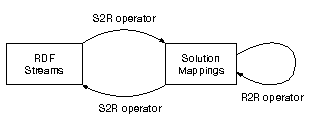
\includegraphics[width=.65\textwidth]{img/cql-rdf-model}\\
    \caption{The CQL processing model adapted for RSP}
    \label{fig:cql-rdf-model}
  \end{center}
\end{figure}

The RDF stream processing model is depicted in Figure~\ref{fig:cql-rdf-model}. It is directly derived from the CQL one (see Section~\ref{sec:CQL}). The stream and the relation concepts are mapped to RDF streams and to set of mappings (using the SPARQL algebra terminology), respectively. To highlight the similarity of the RSP operators \cite{DBLP:journals/ijswis/DellAglioVCC14} to the CQL ones, the same names (\textbf{S2R}, \textbf{R2R} and \textbf{R2S}) are used to indicate the stream-to-relation, relation-to-relation and relation-to-stream operators. 

The concepts described in this section are all implemented in our Streaming Linked Data (SLD) framework (see Section~\ref{sec:sld}) and inspired the definition of our generic streaming Computational Model presented in Chapter~\ref{ch:computational}. 

\subsubsection{RSP-QL} \label{sec:rsp-ql}
%citare cosa prende da SECRET e da CQL
RDF Stream Processor Query Language (RSP-QL) \cite{DBLP:journals/ijswis/DellAglioVCC14} is an extension of SPARQL created to unify existing RSP query languages (i.e, C-SPARQL~\cite{DBLP:journals/ijsc/BarbieriBCVG10}, CQELS~\cite{DBLP:conf/semweb/PhuocDPH11} and SPARQL\textsubscript{stream}~\cite{DBLP:journals/semweb/AnicicRFS12}).
RSP-QL enables user to register continuous queries. The queries are registered once over streams of data and continuously evaluated. Due to the continuous evaluation semantic, a query produces multiple results over time and the instantaneous answer is a composition of the results of each iteration.
RSP-QL is designed following two main requirements: (i) every evaluation of a query over input data produces a unique solution, (ii) RSP-QL, inspired by SECRET(see Section~\ref{sec:secret}), captures the operational semantics of C-SPARQL engine, CQELS and Morph\textsubscript{stream} (see Section~\ref{sec:vel-var-solutions}).
RSP-QL implements the basic concepts of the extensions of SPARQL concepts presented in the Section~\ref{sec:rdf-sparql}.
We start presenting the core concept of the RSP-QL language, the RSP-QL query.

\begin{Definition}
(RSP-QL query) RSP-QL query Q is defined by the tuple (SE,SDS,ET,QF) where
\begin{itemize}
\item SE is an RSP-QL algebraic expression
\item SDS is an RSP-QL dataset
\item ET is the sequence of time instants on which the evaluation occurs
\item QF is the Query Form
\end{itemize}
\end{Definition}

The presence of the time dimension calls for a new notion of RDF dataset, the input data of the RSP-QL query. 

\begin{Definition}
(RSP-QL dataset) An RSP-QL dataset SDS is a set composed by an (optional) default graph, n $(n \geq 0)$ named graphs and m $(m \geq 0)$ named time-varying graphs obtained by the application of time-based sliding windows over $o \leq m$ streams:
\noindent\begin{align*}
SDS =\{G_0, (u_1,G_1), ..., (u_n,G_n),\\
(w_1, W_1(S_1)), ... , (w_j , W_j(S_1)), \\
(w_{j+1}, W_{j+1}(S_2)), ..., (w_k, W_k(S_2)), ..., \\ (w_l,W_l(S_o)), ..., (w_m, W_m(S_o))\}
\end{align*}  
with:
\begin{itemize}
\item $G_0$ is the default time-varying graph
\item $u_p,w_q$ are IRIs $(u_p,w_q \in \mathbb{I})$ for each $p \in [1,n]$ and $q \in [1,m]$
\item $(u_p,G_p)$ identifies a time-varying named
graph, for each $p \in [1, n]$
\item $(w_q , W_q (S_r))$ identifies a named time-based sliding window over an RDF stream, for each $q \in [1, m]$ and $r \in [1, o]$
\end{itemize}
\end{Definition}

In a continuous environment a definition o a time-varying sequence of solution mappings is needed.

\begin{Definition}
(Time-varying sequence of solution mappings)
A time-varying sequence of solution mappings $\psi$ maps time instants $t \in Ti$ to the set of solution mapping sequences:
\noindent\begin{align*}
\psi : T \rightarrow \{\Psi | \psi\, is\, a\, sequence\, of\, solution\, mappings\}
\end{align*}  
\end{Definition}

The RSP-QL evaluation semantic is an evolution of SPARQL evaluation semantic defined taking into account the time dimension.

\begin{Definition}
(RSP-QL evaluation semantic)
Given an RSP-QL dataset SDS, an algebraic expression SE and an evaluation time instant t, we define
\noindent\begin{align*}
eval(SDS(G), SE, t)
\end{align*}  
as the evaluation of SE at time t with respect to the RSP-QL dataset SDS having active time-varying graph G.
\end{Definition}

\subsection{Open Source Solutions} \label{sec:vel-var-solutions}
In the next sections, we present the principal solutions proposed by the Semantic Web community for taming velocity for heterogeneous data. 
In particular, we present vertical RDF Stream Processors developed before the definition of RSP-QL with their own query languages and a couple of distributed implementations. The proposed solution inspired the streaming Computational Model presented in the Chapter~\ref{ch:computational}.

\paragraph{C-SPARQL Engine}
Continuous SPARQL (C-SPARQL)~\cite{DBLP:journals/ijsc/BarbieriBCVG10} is a language to express continuous queries over flowing data in RDF format. It extends SPARQL 1.1 by defining Data Stream Processing operators, including the possibility of defining window over streams of data.
The C-SPARQL engine\footnote{\url{http://streamreasoning.org/resources/c-sparql}} is an open-source software that exploits the C-SPARQL language to enable the registration of continuous queries to be executed over RDF streams.
Its core is based on two sub-components: Esper (see Section~\ref{sec:esper-epl}) and Jena (see~Section~\ref{sec:var-solutions}) . The former is responsible of executing continuous 
operations on the stream, e.g. sliding window to produce RDF graph. The latter periodically executes standard SPARQL query on the RDF stream fragments to produce continuous results.

\paragraph{CQELS}
CQELS-QL~\cite{DBLP:conf/semweb/PhuocDPH11} is a declarative query language that extends SPARQL 1.1 grammar with operators to deal with streaming data. Continuous Query Evaluation over Linked Streams (CQELS) interpret queries in CQELS-QL and, differently from C-SPARQL, supports only the Istream relation-to-stream operator (see Section~\ref{sec:CQL}).
CQELS offers a flexible framework for the query operations with a dynamic adapting processors that continuously reorders operators to improve query execution in terms of delay and complexity.
It natively implements the query operators in order to limit the overhead and the limitations related to the usage of other engines (e.g. C-SPARQL engine relies on Esper and Jena).

\paragraph{Morph\textsubscript{stream}}
SPARQL\textsubscript{stream}~\cite{DBLP:conf/semweb/CalbimonteCG10} extends SPARQL to support all the stream operators (e.g. sliding window).
SPARQL\textsubscript{stream} is implemented in Morph\textsubscript{stream} engine that exploits Ontology-Based Data Access techniques~\cite{DBLP:journals/ijswis/CalbimonteJCA12}.
Morph\textsubscript{stream} execution is based on R2RML\footnote{\url{https://www.w3.org/TR/r2rml/}} mappings between ontologies and data streams.
The queries are first rewritten in a relational algebra expression with time window extension and then translated in the Data Stream Processing target language.

\paragraph{INSTANS}
Incremental eNgine for STANding Sparql (INSTANS) \cite{DBLP:conf/semweb/RinneNT12} enables users to create a flow of multiple SPARQL 1.1 queries that represents a single task. The engine is in charge of continuously evaluates the incoming data and store intermediate results. INSTANS approaches RDF stream processing from a different perspective and does not require a continuous extensions to RDF or SPARQL.

\paragraph{ETALIS and EP-SPARQL}
Event TrAnsaction Logic Inference System (ETALIS) \cite{DBLP:journals/semweb/AnicicRFS12} is an RDF stream processing engine that takes in account two time-stamps during the data processing.
It is a pluggable system that can use multiple prolog engines.
An internal ETALIS task can be specified using two different languages, Event Processing SPARQL (EP-SPARQL) and ETALIS Language for Events (ELE). Both of them allow users to derive complex events through deductive prolog rules. 
The engine supplies the results as soon as they are available and supports three different policies during the execution of the task: (i) unrestricted, all the input items are used for matching the declared patterns; (ii) chronological, the earliest matchable input are selected for matching the event patterns, the next evaluations will ignore the already selected data; (iii) recent, the latest matchable input are selected for matching the event patterns, as for chronological policy, they are then ignored.

\paragraph{CQELS Cloud}
CQELS Cloud~\cite{DBLP:conf/semweb/PhuocQVH13} presents an elastic and distributed environment that exploits an extension of CQELS to enable a network of processing nodes to parallelize tasks.
The input of the CQELS Cloud execution model is a set of CQELS-QL queries to be executed against a set of RDF input streams and the output is a set of output streams (in RDF or relational format).
The input queries are compiled to produce a logical query network that defines the algebras for each input stream. The logical query network is, then, mapped on a processing network made of processing nodes, namely the Operator Containers (OCs). The tasks are distributed among the OCs by the Global Scheduler.

\begin{figure}[h]
\begin{center}
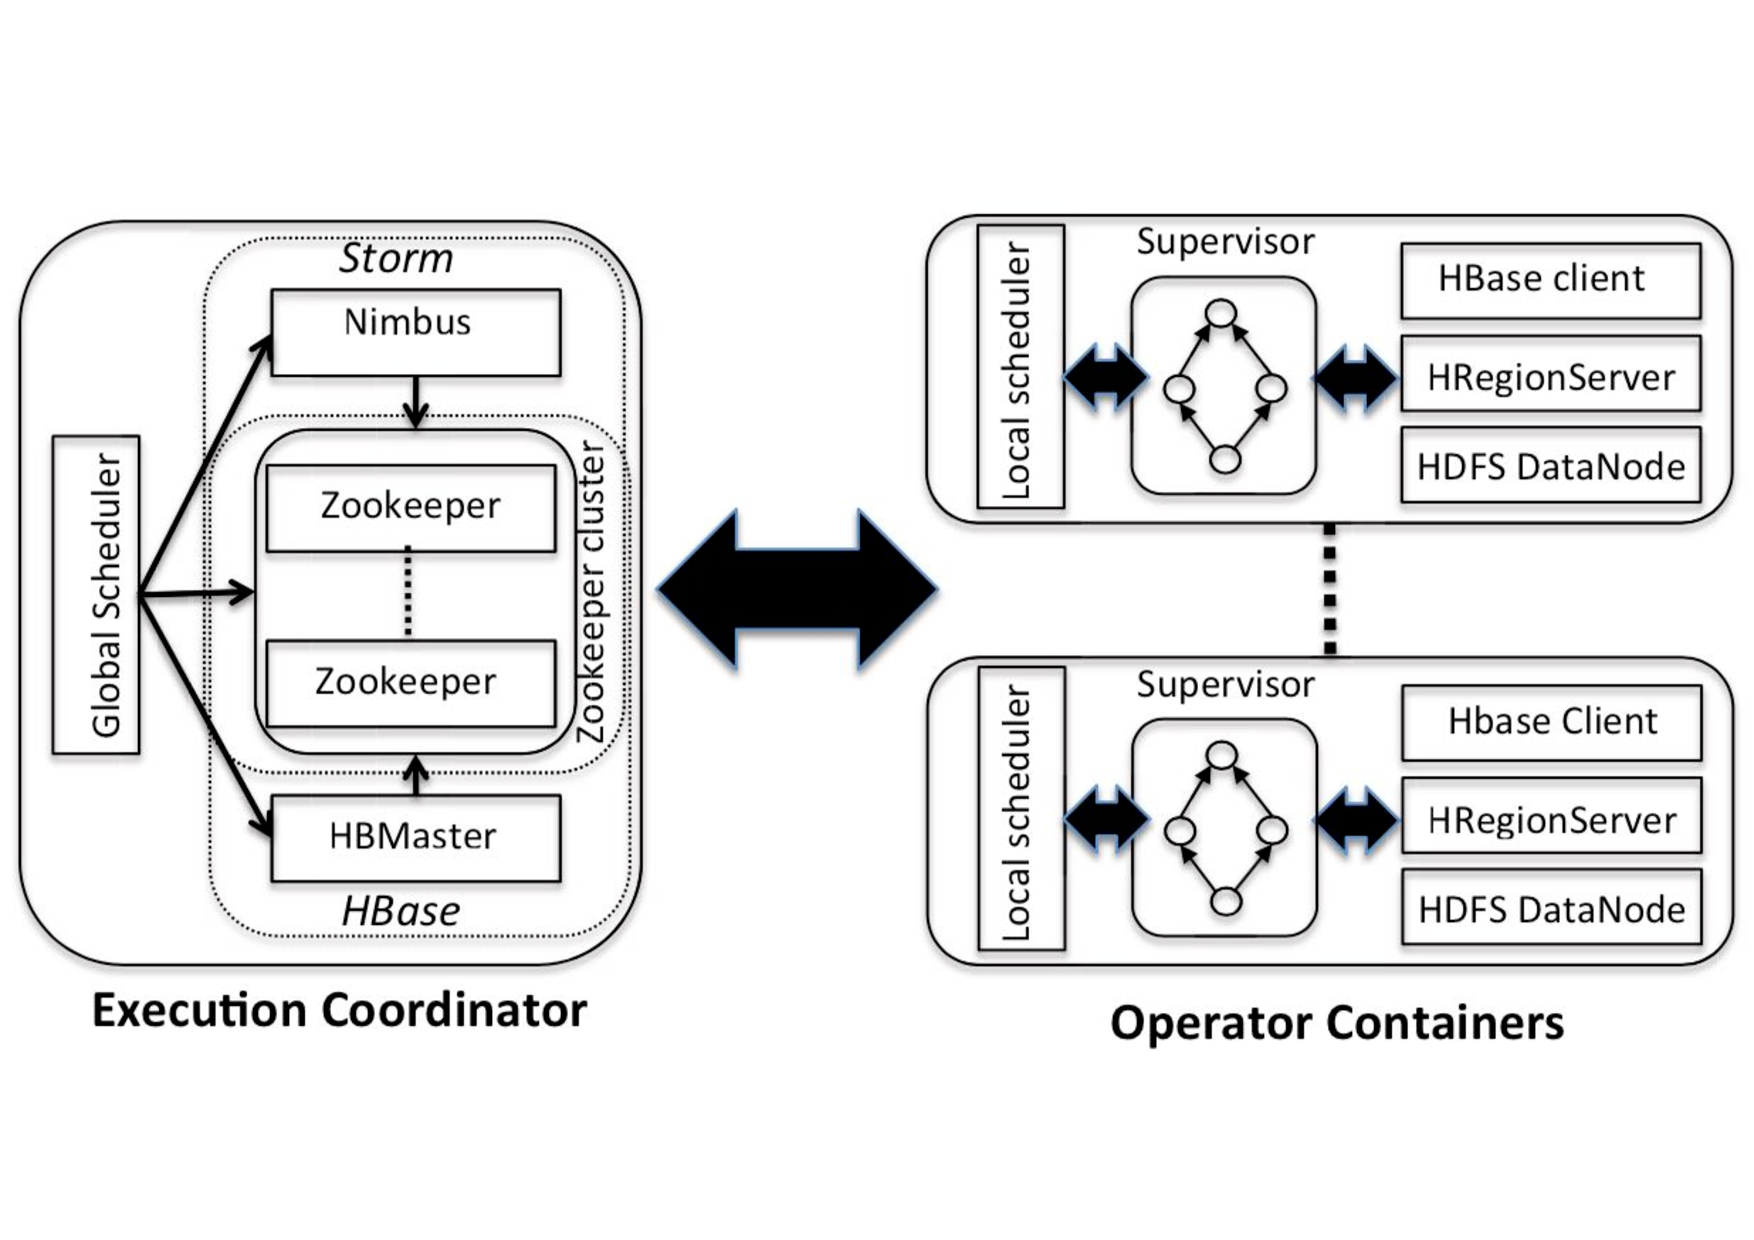
\includegraphics[width=0.85\textwidth]{img/cqels-cloud}
\caption{CQELS Cloud architecture (source~\cite{DBLP:conf/semweb/PhuocQVH13}).}
\label{fig:cqels-cloud}
\end{center}
\end{figure}

Figure~\ref{fig:cqels-cloud} depicts the general architecture of the system. CQELS Cloud implements the elastic execution model and the parallel algorithms exploiting ZooKeeper~\cite{DBLP:conf/usenix/HuntKJR10}, Storm\footnote{\url{http://storm-project.net/}} and HBase\footnote{\url{http://hbase.apache.org/}}. 

\paragraph{Strider}
Strider \cite{DBLP:conf/semweb/RenC17} is a distributed and adaptive RDF Stream Processing engine that optimizes logical query plan according to the data stream evolution developed to guarantee scalability, availability, fault-tolerance, high throughput and acceptable latency. 

Strider relies on well known distributed technology and is composed by two main components: (i) the data flow management and (ii) the Computing core. 
The former is based on Apache Kafka, it categorizes the input RDF streams into different message topics which represent the different family of RDF events.
The latter is based on the Spark Streaming framework, it creates a pipeline to perform parallel processing on the messages emitted by Kafka.

Strider proposes static and adaptive optimization components based, respectively, on heuristic rules and (stream-based) statistics and two strategies for the Adaptive Query Processing (AQP): backward (B-AQP) and forward (F-AQP) that mainly differ on the query plan computation time (i.e. at the previous or current window).

\section{RSP Middleware}\label{sec:rsp-mid}
RSP Middlewares ease the task of deploying the RSP Engine in real-world applications by offering extensible means for collecting data in real-time, for publishing, accessing and querying collected information as Linked Data, and for visualizing query results. 

In the next sections we present two different implementations of an RSP Middleware (the Streaming Linked Data (SLD) framework~\cite{DBLP:conf/semweb/BalduiniVDTPC13} and the Linked Stream Middleware~\cite{DBLP:journals/ws/PhuocNPH12}). They approach the problem in different ways. 
The SLD framework adopts a data driven in-memory approach for the processing of RDF streams with limited support for static information, the Linked Stream Middleware is a cloud-based infrastructure to integrate time-dependent data with other Linked Data sources. 

\subsection{Streaming Linked Data (SLD)} \label{sec:sld}
The Streaming Linked Data (SLD) framework is a general-purpose, pluggable system that supports the development of applications that continuously analyse RDF streams.
SLD is designed to address five different requirements:

\begin{itemize}
\item[\textbf{(R1)}] \emph{every input is an RDF data stream}. The system must indifferently ingest data with different velocities from any sources. All the incoming information is modeled as an RDF data stream. 
\item[\textbf{(R2)}] \emph{Continuous Ingestion}. The continuous nature of data streams requires a continuously capture phase. The data, once arrived, is marked with an increasing timestamp. The system could handle data arriving with its own time mark.
\item[\textbf{(R3)}] \emph{publish/subscribe}. SLD enable a publish/subscribe logic for its components. A senders, the \textsf{publishers}, publish timestamped RDF triples into RDF streams,  and receivers, the \textsf{subscribers}, listen to one or more RDF streams, and only receive timestamped RDF triples that are of their interest. Publisher and subscribers do not have to know each other.
\item[\textbf{(R4)}] \emph{reliable message-passing}. SLD implements a logically reliable message-passing system that guarantees timestamped RDF triples to be delivered in order.
\item[\textbf{(R5)}] \emph{minimizes latency by using main memory}. SLD minimizes latency by using main memory and avoiding disk I/O bottlenecks.
\end{itemize}

\begin{figure}[h]
\begin{center}
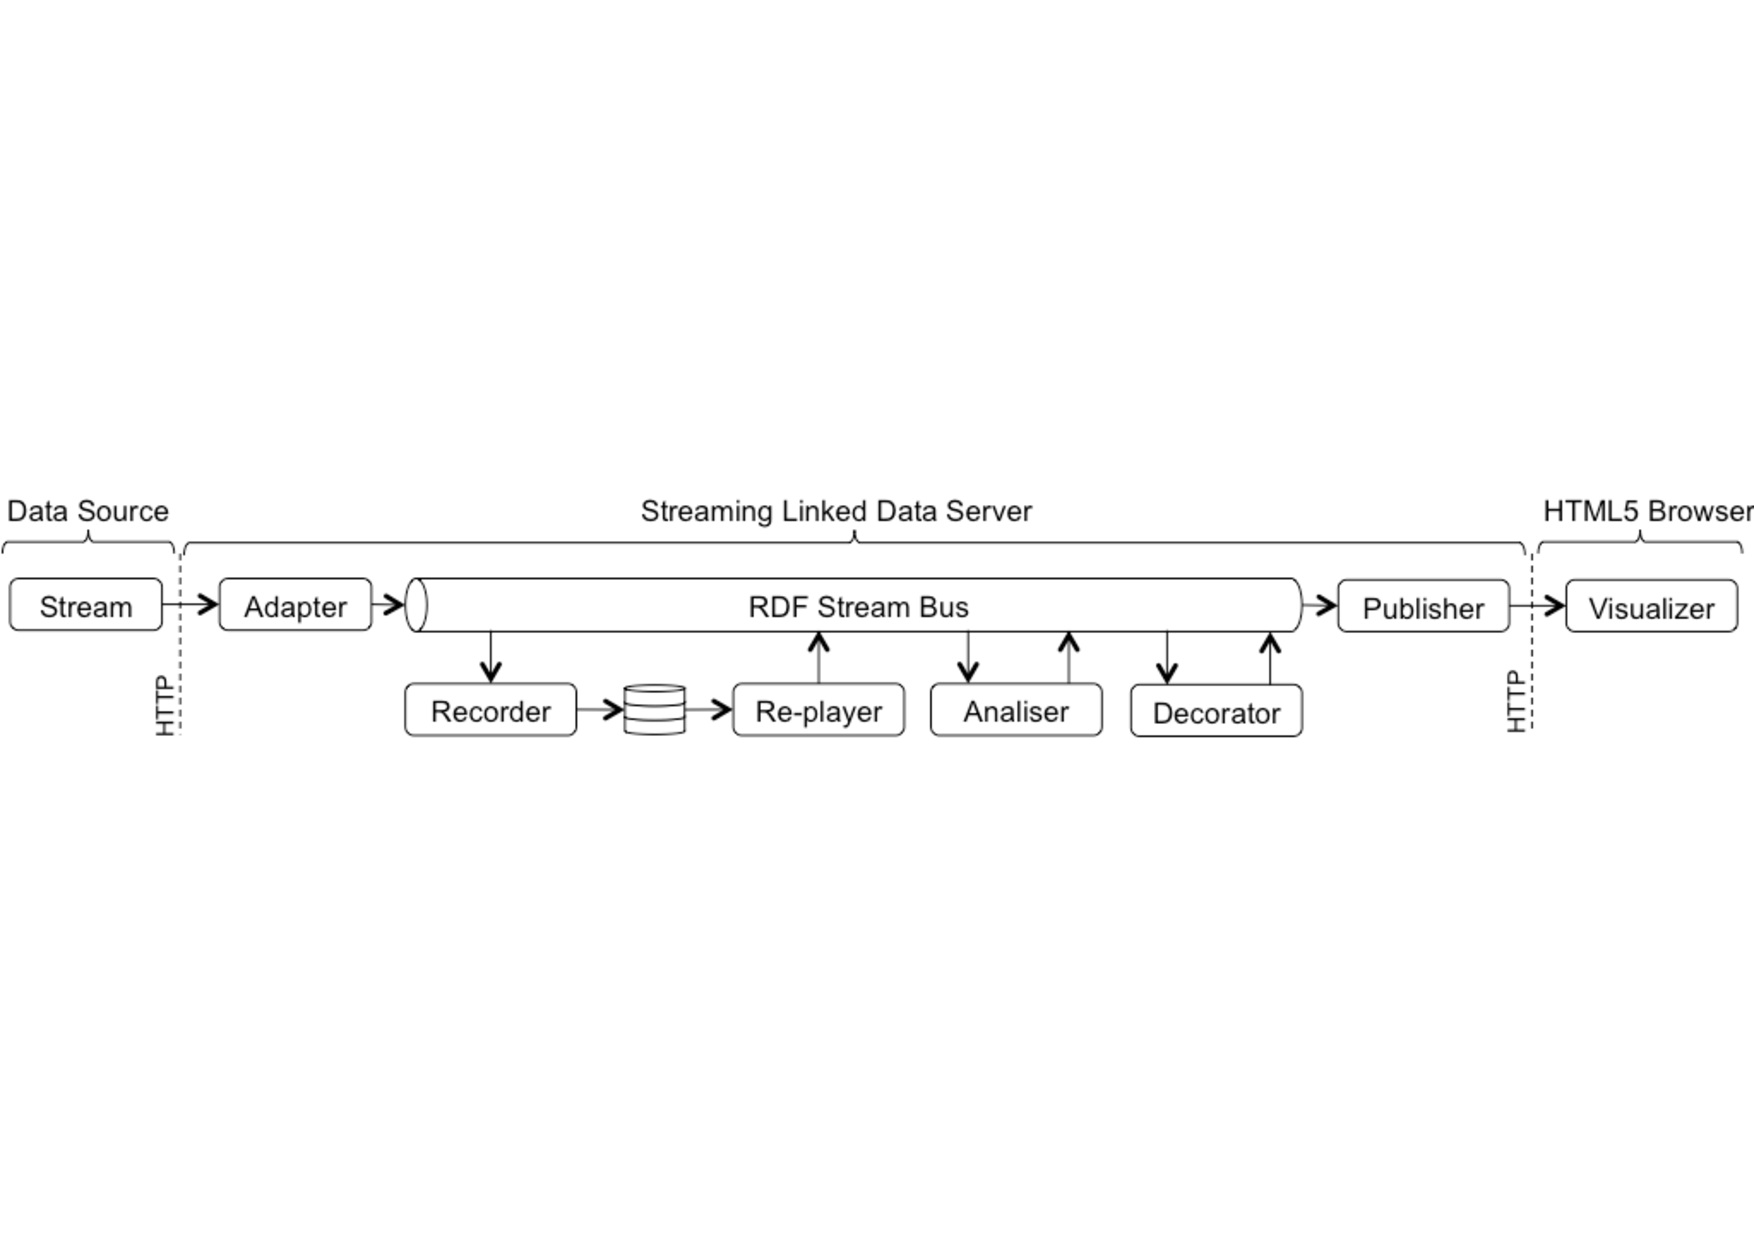
\includegraphics[width=1\textwidth]{img/SLD-arch}
\caption{The architecture of the Streaming Linked Data framework.}
\label{fig:sld-arch}
\end{center}
\end{figure}

Figure \ref{fig:sld-arch} illustrates the architecture of the SLD framework.  The leftmost column logically contains the \emph{streaming data sources}, the central one the SLD server, and the rightmost one the visual widgets to be embedded in a dashboard. 

The \emph{streaming data sources} are assumed to be distributed across the Web and accessible via HTTP.

The core of the framework is \emph{SLD Server}. It includes  components for accessing data stream sources, internally streaming data, registering and replaying portion of data streams,  decorating and analysing time-boxed portion of the stream, and publishing the results. 

The \textsf{adapters} allow to access data stream resources, possibly delegating filtering operations to the data source, and to translate data items in the stream into set of timestamped RDF triples. SLD framework includes adapters for different social networks (e.g., Twitter, Instagram, foursquare) and for several sensor networks. For instance, the Twitter adapter allows to push to Twitter either geo-spatial filters, which ask Twitter to stream to SLD only tweets posted from given locations, or keyword-based filters, which ask Twitter to stream to SLD only tweets containing one or more of such key-words. Each tweet is internally represented using the extension of SIOC ontology presented in \cite{DBLP:journals/ws/BalduiniCDVHLKT12}. 

The \textsf{publishers} make available on the Web the content of chosen RDF stream following the Linked Data principles \cite{DBLP:journals/ijswis/BizerHB09} in the Streaming Linked Data format proposed in \cite{DBLP:conf/www/BarbieriV10}. The format is based on two types of named RDF graphs: instantaneous Graphs (iGraphs), which contain a set triples having the same timestamp, and stream graphs (sGraphs), which contains triples that point to one or more timestamped iGraphs. The number of iGraphs pointed by an sGraph and their time interval of validity can be configured when instantiating the publisher.

The \textsf{recorders} are special types of publishers that allow for persistently storing a part of an RDF stream. As format, we used an extension of the Streaming Linked Data format based on iGraphs and recording graphs (rGraphs). The latter are similar to sGraphs, but they include pointers to all the iGraph recorded and such pointers do not have a time interval of validity. The \textsf{re-players} can inject in an RDF stream what recorded in an rGraph.

The \textsf{analysers} continuously observe the timestamped triples that flow in one or more RDF stream, perform analyses on them and generate a continuous stream of answers. SLD framework includes a built-in engine that executes C-SPARQL queries, but any of the aforementioned continuous extensions of SPARQL (see Section~\ref{sec:vel-var-solutions}) can be plugged in SLD server and used for the analysis. 

The \textsf{decorators} are special types of analysers that look for a pattern of triples in a RDF stream. When the pattern matches, the decorators run a computation of the matching and add new triples to the stream.

SLD represents the first attempts to create a streaming computational model with the definition of generic principles related to the RDF stream processing world. SLD inspires the generic streaming computational model presented in the Chapter~\ref{ch:computational}.

\subsection{Linked Stream Middleware}
Le-Phuoc et al.~\cite{DBLP:journals/ws/PhuocNPH12} proposes Linked Stream Middleware (LSM), a platform to create a bridge between data streams and Semantic Web.
LSM offers: (i) a wide range of extendable wrappers to access streaming sources and transform the raw data into Linked Stream Data~\cite{DBLP:conf/semweb/SequedaC09}, (ii) components for annotating and visualizing data through a Web interface and live querying functionalities over unified Linked Stream Data and data coming from the Linked Open Data cloud exploiting a standard SPARQL query processor and CQELS.

\begin{figure}[h]
\begin{center}
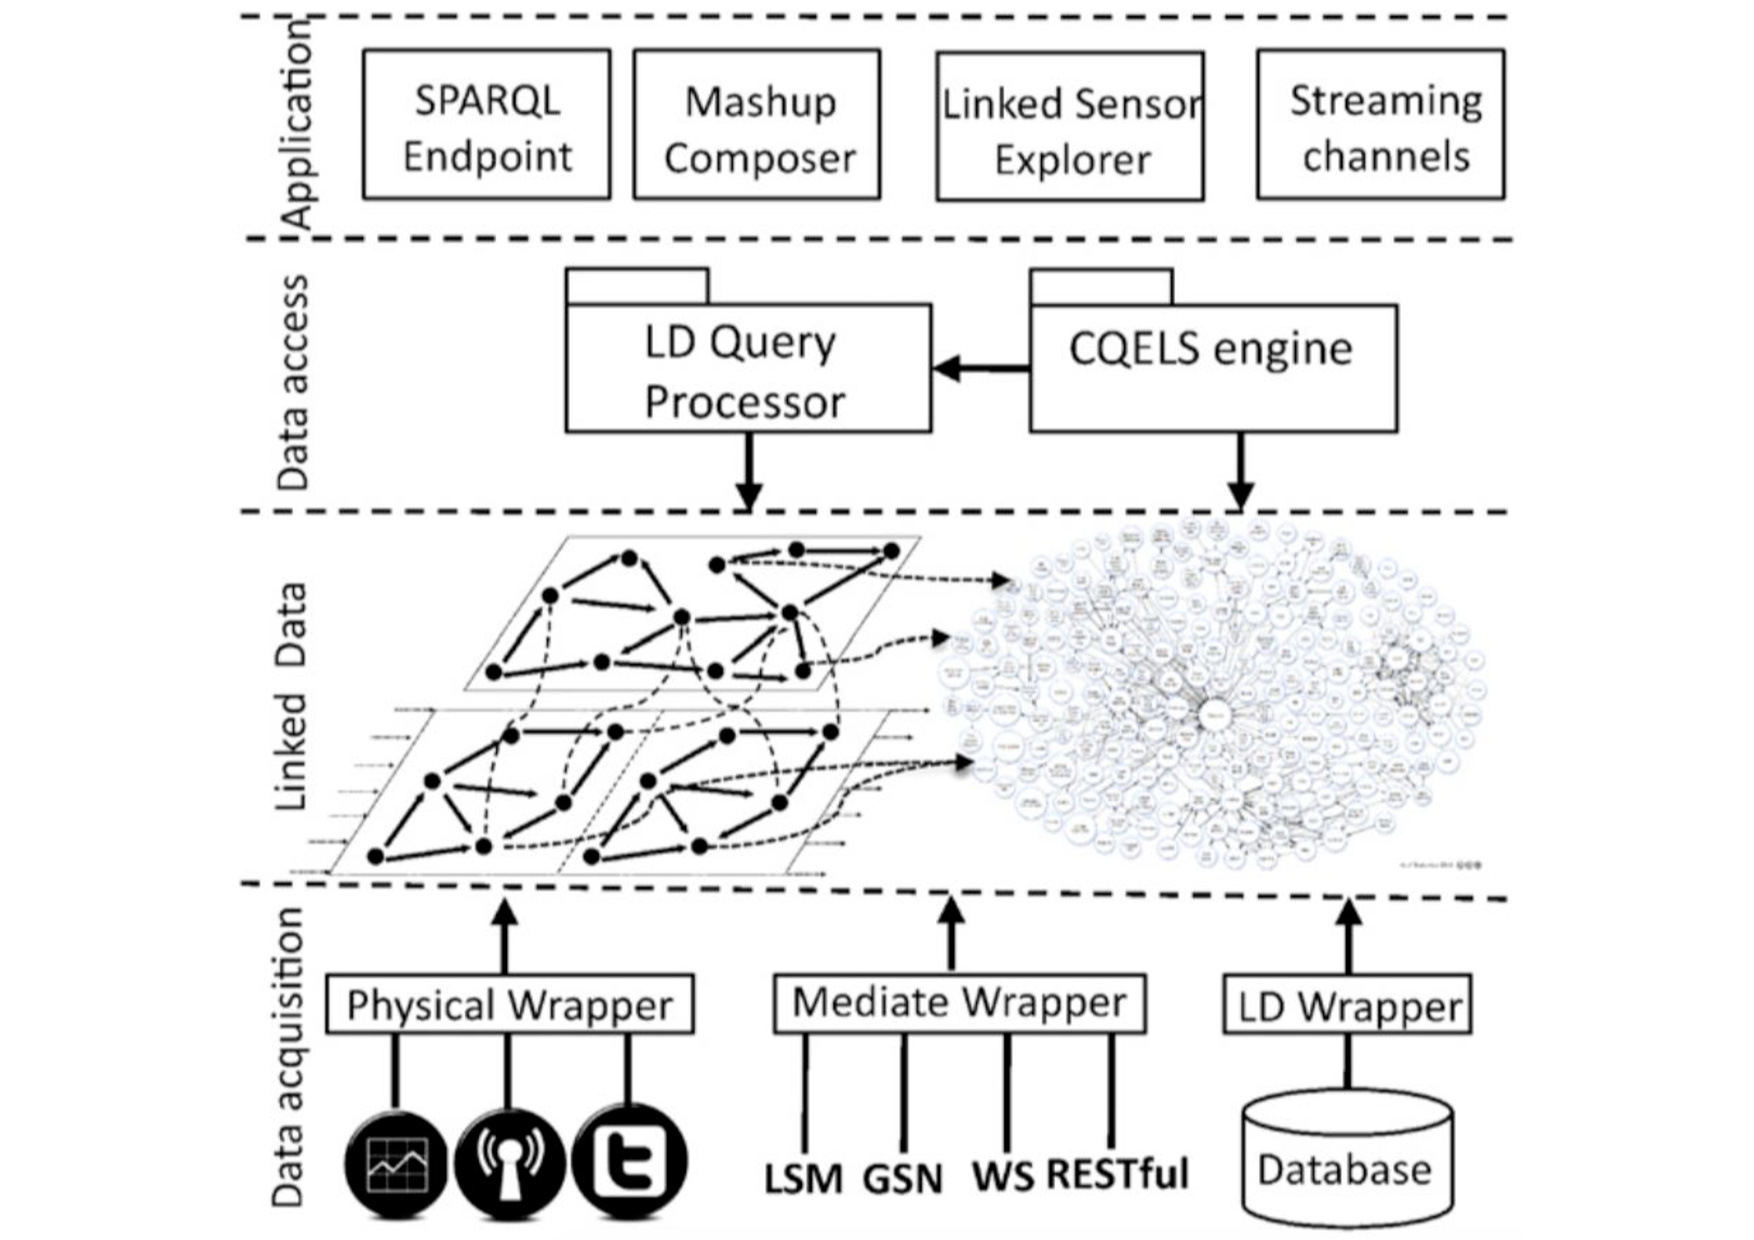
\includegraphics[width=0.7\textwidth]{img/lsm}
\caption{Linked Stream Middleware architecture (source~\cite{DBLP:journals/ws/PhuocNPH12})}
\label{fig:lsm-arch}
\end{center}
\end{figure}

The LSM architecture is layered to increase scalability and flexibility, Figure~\ref{fig:lsm-arch} presents an overview of LSM middleware.

The \textit{Data Acquisition layer} is in charge of collecting data from streaming data sources via a wide range of wrappers. The different characteristics of the proposed wrappers allows the system to cover a broad range of input format. The output of the wrappers conforms to format described in the Data Access Layer. The system allows users to develop their own wrapper in order to guarantee the flexibility of the entire system.
The \textit{Linked Data layer},  following the Linked Data publishing principles presented in~\cite{DBLP:series/synthesis/2011Heath},  adds a global identifier to the data to ensure the data composability and exploits an ontology to represent data in a triple-based format. In particular LSM use the Semantic Sensor Network (SSN) Ontology\footnote{\url{http://purl.oclc.org/NET/ssnx/ssn}}.
The \textit{Data Access layer} enable declarative query answering on top of the Linked Data layer  in a pull-based or push-based fashion. This layer enables the storage of stream data and metadata in a triple format to ease the access of historic data.
The \textit{Application layer} offers support for developing applications to exploit query processing capabilities of the Data Access layer. The layer offers a SPARQL Endpoint, a Linked Sensor Explorer, a Mashup Composer and Notifications/Stream channels and enables query operation on historical sensor data. Continuous queries can be registered into the system to populate user-defined output streams.

\section{Benchmarking}\label{sec:benchmarking}
In this section, we propose an overview the benchmarking principles. In particular, Section~\ref{sec:dsb} introduces \textit{domain-specific} benchmarks. Section~\ref{sec:vel-bench}, then, concentrates on the benchmarking of velocity oriented systems, i.e., systems created to deal with continuously flowing data (e.g., RSP). Finally, Section~\ref{sec:bench-cost} casts some light on the innovative concept of Configuration that Outperforms a Single Thread (COST), showing that a distributed solution, to be effective, must outperform a single-threaded one.


\subsection{Domain-Specific Benchmarks}\label{sec:dsb}
Nowadays, the variety of application of computer systems are growing faster than ever.
A single metric cannot measure and evaluate the performance of a computer system in all applications and domains.
A computer system is generally designed to face few problem domains and the performance in performing other tasks can be very poor.
Jim Gray~\cite{gray1992benchmark} proposes the \textit{domain-specific} benchmarks concept as a response to the heterogeneity of computer system use. 

A benchmark, built according to this concept, specifies a synthetic workload shaped to evaluate a system while it performs a typical application for which it was designed.
A \textit{domain-specific} benchmarks must follow four criteria. It must be: 
\begin{itemize}
\item \textit{Relevant}: given the problem domain, the benchmark must measure the peak performance and price/performance of the system during a typical domain-specific operation.
\item \textit{Portable}: the benchmark should be easy to be implemented on different systems and architectures.
\item \textit{Scalable}: the benchmark should apply to small and large computer systems, it should be also possible to test system on parallel architecture. 
\item \textit{Simple}: to ensure the credibility of the system, it must be understandable.
\end{itemize}

As stated in the principles, Gray \cite{gray1992benchmark} highlights the importance of price/performance metrics for system benchmarking.
The next sections will highlight the existing works on benchmarking streaming systems and the cost-aware approach.

\subsection{Benchmarking Velocity Oriented Systems}\label{sec:vel-bench}
The most relevant benchmark effort related to data stream management systems is the Linear Road benchmark~\cite{arasu2004linear}. In this work the authors present a benchmark specification for data management system with continuous querying capabilities. The benchmark is based on a traffic simulation use case. The system under test must answers queries from the vehicles on the road network in simulated real-time. The specification includes I/O, queries, expected results and relevant metrics for the system under test.

In many contexts, performance is very relevant. One of the first benchmarks for distributed streaming data processing is the Yahoo Streaming Benchmark~\cite{chintapalli2016benchmarking}.
This benchmark is based on a realistic use case. Also, a complete pipeline is implemented, from data ingestion to results. 
It is focused on performance metrics, namely latency and throughput, and it does not consider cost in its comparison. The benchmark code is available online under the Apache 2.0 license\footnote{https://github.com/yahoo/streaming-benchmarks}.

A more recent work on comparing popular distributed processing engines can be found in~\cite{karimov2018benchmarking}. This work presents a performance comparison for Apache Storm \cite{toshniwal2014storm}, Apache Flink \cite{carbone2015apache} and Apache Spark~\cite{zaharia2016apache}. The comparison is based on realistic industrial use cases, and it focuses on throughput and latency.

The correctness theme pushed the discussion on what is really important in a dsb for Stream Reasoning~\cite{DBLP:conf/esws/ScharrenbachUMVB13}.
Dell'Aglio et al.~\cite{DBLP:conf/semweb/DellAglioCBCV13} propose a formal characterization of the operational semantics of different RSP (i.e. C-SPARQL Engine, CQELS, SPARQL\textsubscript{stream} and EP-SPARQL) exploiting CQL and SECRET. This formalization allows to determine a concept of correctness in RSP domain and to develop CSRBench~\cite{DBLP:conf/semweb/DellAglioCBCV13} an extension of SRBench~\cite{DBLP:conf/semweb/ZhangDCC12} to address query result correctness verification using an automatic method.
Along the same line, Ali et al.~\cite{DBLP:conf/semweb/AliGM15} and Kolchin et al.~\cite{DBLP:conf/icwe/KolchinWKT16} propose workloads and software environments to run experiments and perform measurement of quality criteria.
A recent work of Tommasini et al.~\cite{DBLP:conf/esws/TommasiniVBD16} proposes an open-source test-stand to ensure the reproducibility of experiments.

The performance metrics plays a key role in the evaluation (see Section~\ref{sec:comp-mod-eval-performace}) of the implementations of our streaming Computational Model presented in Chapter~\ref{ch:computational}

\subsection{Cost-Aware approach}\label{sec:bench-cost}
Recently, in the Distributed System community, the concept of Configuration that Outperforms a Single Thread, namely COST, is gaining importance. 
McSherry et al.~\cite{mcsherry2015scalability} introduce the COST metric and demonstrate that a single-threaded implementation of popular graph algorithms outperforms all distributed graph processing engines by orders of magnitude, at a fraction of the cost. Similarly, Boden et al. \cite{bodendistributed} compare single-threaded implementations of common machine learning algorithms with their distributed counterparts. Those are implemented using the most popular distributed machine learning libraries.

The concept of COST plays a crucial role in the evaluation (see Chapter~\ref{sec:comp-mod-eval-cost}) of the different implementations of the Computational Model proposed in Chapter~\ref{ch:computational}




 
%Urban data analysis
\chapter{Urban Data analysis}\label{ch:uda}

In this chapter, we introduce the state-of-the-art on urban data analysis.
We justify the choice of urban data as a privileged form of spatio-temporal data useful for a PhD thesis like this one, due to its variety and availability.
Section~\ref{sec:uda-motivation} presents relevance and motivations of the urban data analysis with an overview of the most important research works in the field.
In Section~\ref{sec:uda-analysis}, we present the different dimensions of urban data analysis, related to content, time and space (and a combination of them).
Section~\ref{sec:uda-solution} presents an overview of relevant examples of implementations of RDF stream processing concepts at work on urban data.
RSP represents a suitable solution because of the variety and velocity of the data sources and because of the need to fuse static (slowly evolving) and streaming data.
The first examples (see Section~\ref{sec:uda-starcity} and Section~\ref{sec:uda-trafficlark}) exploit data from different urban sources and the capability of RSP to abstract the real nature of the data through OBDA (see Section~\ref{sec:obdi-obda}) that helps the machinery and the final user to extract insights from data.
The two examples in Section \ref{sec:uda-bottari} and in Section \ref{sec:uda-london}, mainly exploit data from Twitter. The data from social network has an intrinsic graph nature and was extracted using the official APIs that return the data in JSON format. Therefore, it is easy to transform it in JSON-LD\footnote{\url{https://json-ld.org/}}, a format compatible with Semantic Web technologies. The usage of an RDF stream processor in this scenario is natural.

\section{Relevance and Motivation}\label{sec:uda-motivation}
The relevance of urban computing, or urban informatics, has been recognized since long. A recent survey on urban sensing \cite{DBLP:journals/csur/CalabreseFB14} clearly shows the value of mobile phone data to get insights of urban dynamics and human activities. 

Studies like Gonzalez et al.~\cite{gonzalez2008understanding} focus on using the mobile phones data, namely the call data records (CDRs), to track individual motion patterns characterizing each individual using a time-independent travel distance parameter and a significant probability to return to a few highly frequented locations. Candia et al.~\cite{candia2008uncovering} investigate patterns of calling activity at the individual level and show that the inter-event time of consecutive calls is heavy-tailed. 
In recent years, the analysis of telco data in such an individual way rises serious privacy issues.

However, it is also possible to use telco data in privacy preserving way.
A common applications is to use CDRs to estimate the density of crowds and vehicles in different urban regions~\cite{mcardleanalyzing,caceres2012exploring}. Another example involves the detection of people habits. Ratti et al.~\cite{ratti2006mobile} present the Mobile Landscape project, one of the first urban analysis based on the geographical mapping of cell phone usage at different times of the day in the metropolitan area of Milan. Becker et al.~\cite{becker2011tale} capture key mobility patterns within Morristown, NJ, by identifying users' home and work locations from CDRs. This information is particularly useful for urban managers and authorities that are responsible for efficient public transportation systems. Also De Nadai et al.~\cite{de2016death} test the four Jacobs conditions\footnote{The four conditions exposed by Jane Jacobs in~\cite{jacobs1961death}: mixed land uses, small blocks, buildings diversity in terms of age and form and sufficient dense concentration of people and buildings} that promote life in cities by using CDRs. Wesolowski et al.~\cite{wesolowski2013impact} combine CDRs with other cellphone-related logs (e.g., tower pings, cellular handovers) in order to compare human mobility patterns derived from CDRs.

Although mobile phones data is a priceless source to gather underlying patterns of cities and their citizens, they have got some limitations since they cannot reveal any information about people interests and thoughts. Social media data represents an opportunity to access information at individual level without violating privacy. This data is, indeed, made public by the user through a self determination process.
Social media streams are a powerful mean to explore people opinions and preferences with regard to specific venues and events.
For instance, Hristova et al.~\cite{hristova2016if} analyze temporal, spatial, and microeconomic patterns of sport game attendees to understand the users' dynamics, while Lee et al.~\cite{lee2016not} and Cho et al.~\cite{cho2011friendship} use social networks and cell phone location data, to identify humans' mobility patterns. Psyllidis et al.~\cite{psyllidis2015platform} concentrate their effort on wide range of urban data and create a web-based platform to support city planning and decision-making. In particular, Singh et al. \cite{singh2010social} introduce the concept of \textit{social pixel} that aggregates social interests of users about particular themes and locations. 
This notion plays a key role during the development of our conceptual model presented in Chapter~\ref{ch:conceptual}.

Moreover, urban data from different sources (e.g., CDRs, social data, IoT, etc.) can be merged to reveal even more interesting insights on city dynamics and urban monitoring. 
The platform built by Calabrese et al.~\cite{calabrese2011real} combines the users' mobile phones' data with the real-time location of buses and taxis to model the car traffic in Rome. Botta et al.~\cite{botta2015quantifying} try to quantify the dimension of the crowd by exploiting a combination of CDR and social media data.
Quercia and his colleagues \cite{quercia2011mobile} use CDRs to study human mobility related to special planned events in Boston. Calabrese et al. \cite{calabrese2010geography} show that there is a high correlation between the kind of event, e.g., sport, theater, music, family events, and the home location area of its attendees. Quercia et al. \cite{quercia2010recommending} build a recommendation system for social events and find out that the most effective algorithm recommends those events that are popular among local residents.

Sentiment analysis covers a wide range of applications in cities. Authors in \cite{ahmed2016smart} propose a city sensing architecture from Twitter data to monitor user opinions about events and topics. Hawelka et al. \cite{hawelka2014geo} and Calabrese et al. \cite{calabrese2010human} analyze geo-located Twitter messages and geographical preferences in order to predict global patterns of human mobility.

One of the features of interest for policy makers and cities managers~\cite{habitat2016urbanization} is the extremely diversified composition of the language mix, or multilingualism. This interest is motivated by the increasing immigration flows towards cities~\cite{sanderson2015world}, which result in rapidly changing population density~\cite{deville2014dynamic}. Multilingualism has also a broad scope in academia. In particular, different papers approach the issue of multilingualism from a historical perspective. Leimgruber in \cite{leimgruber2013management}, for example, analyses the city of Singapore, Garcia et al.~\cite{garcia2001multilingual} the city of New York, Extra et al.~\cite{extra2004urban} develop a cross-linguistic perspective on Gothenburg, Hamburg, The Hague, Brussels, Lyon and Madrid.
Moreover, Tasse et al.~\cite{tasse2016generating}, Arnaboldi et al.~\cite{arnaboldi2016studying} and Bokanyi et al.~\cite{bokanyi2015race} characterize cities and their neighborhoods from different aspects namely safety, culture and demographics through social media networks. Quaggiotto et al. \cite{quaggiotto2010new} present a tool called City Murmur with the aim at showing how different media describe the urban space through the attention that is payed on each street of a city. It wants to build a time-based narration, an historical archive of media coverage of the urban space which is able to reveal some hidden dynamics useful for city policy support, critical media analysis, and sociocultural research.

The interest around the exploitation  of urban data are growing, however the joined use of multiple data sources has not yet been fully explored.
In the next sections, using technologies meant to tame velocity and variety simultaneously (see Section~\ref{sec:rsp-mid}), we present different use cases of urban streaming data analysis.

\section{Urban Data Analysis Dimensions} \label{sec:uda-analysis}
The urban data analysis can be developed on three different dimensions: \textbf{space}, \textbf{time}, and \textbf{content}. In this section, we summarize the characteristic of each analysis dimension. See Section~\ref{sec:conc-fr-2-analysis} for more information about how our conceptual model (proposed in Chapter~\ref{ch:conceptual}) enables the described analysis dimensions

\subsection{Content Analysis}
The content can be associated to an event and thus indirectly to the time and space of the happening, and carries information that represents a measure of intensity of a tracked event.
During a content based analysis of urban data, a stakeholder can be interested about the contextual and behavioral knowledge about what and how users share about an event. 

The content analysis can be approached in two different ways: (i) using the \textit{Original} content, or (ii) creating \textit{Augmented} content.
In the former approach, the original content is analyzed as is and used for profiling social media users who are engaged in events. In the latter one, the augmented content can be created by using concept and feature extraction techniques from the original content for the purpose of more complex analysis about the events and their attendees.

The augmented content could consist of different media types including text, image, video, etc. that also contain low-level information about events like locations, time tables, related social users and so forth. From such content, \textbf{low-level features} such as color schema for images or n-gram distribution for text, can be extracted. For instance, a system can use the main color schema in photos related to an event to verify the correctness of the estimated location of that event. Furthermore, \textbf{high-level features} like number of people and their demographics in a photo, list of existing concepts that are represented in a photo or a video (using deep learning techniques) or semantic entities from text using ontology-based matching, can be extracted.

\subsection{Spatial Analysis}
Another dimension of interest in city analyses is space. Therefore, a urban analytics system must focus on analyzing events, people presence and flow, content and opinion sharing, or any other type of phenomena (like electrical consumption, traffic, economical value) with respect to the spatial distribution and spreading, also considering its dynamics in time. 
The spatial dimension is more complex to deal with than one can expect. Indeed, in smartcity context, the data sources may vary a lot: some information may refer to specific geographical points (geo-coordinates), some others may refer to venues or locations (restaurants or other public or private spaces), while others can provide information referring  to broad areas, possibly with different size and shape. Any analysis considering two or more different data sources need to keep this into account.

Interesting types of relevant analysis categories can be:
\begin{enumerate}
\item \textit{Dispersion}: studying the spatial distribution of locations of events, in particular with respect to the deviation from purely random configuration. This can be achieved with measures such as the Gini coefficient~\cite{yitzhaki1983extension}.
\item \textit{Distance and relation to places}: studying the spatial relation of events with respect to a set of given locations (e.g., stores or venues for specific happenings such as fashion shows, see Section~\ref{sec:cs-mfw}). This is covered by simple measures such as the average Euclidean distance between event and location, or the average Manhattan distance over an artificial grid of cells or travel distance over the road network.
\item \textit{Correlation}: studying the relevant correlations between different signals along the space dimension (e.g, within and across administrative boundaries). 
\item \textit{Prediction}: defining predictive analytics along the space dimension, by analyzing historic series of data and comparing it with the most fresh information from given geographical area.
\end{enumerate}

\subsection{Temporal Analysis}
Temporal analysis focuses on the study of the evolution and spreading of signals over time (e.g., measuring how fast information about an event propagates). 
The goals of temporal analysis can be diverse. We identify the following types of relevant analysis categories:
\begin{enumerate}
\item \textit{Description}: consisting in defining the signal as a time series in order to have a view of the evolution of information flows over time.
\item \textit{Correlation}: studying the temporal correlation between different time series and infer common behaviors and dynamics.
\item \textit{Prediction}: allowing generating temporal prediction over observed or correlated phenomena.
\item \textit{Anomaly detection}: identifying discrepancies between expected temporal behaviors and actual happenings.
\item \textit{Causality}: determining possible causality relations between different events.
\end{enumerate}

\subsection{Combined Time and Space Analysis}
Given the basic space and time analysis aspects described above, the subsequent level of interest is the combined analysis along both directions. A system can combine techniques described in the previous sections for running analysis across time and space. 

Furthermore, one can define time series of values that are aggregated or calculated on geographical basis. For instance, a system can define the time series of the values of the Gini Index or of the average distance of events from a set of given venues, and then analyze them along the temporal axis. 

\section{Existing Semantic Web-Based Solutions}\label{sec:uda-solution}

\begin{figure}[t!]
	\centering
	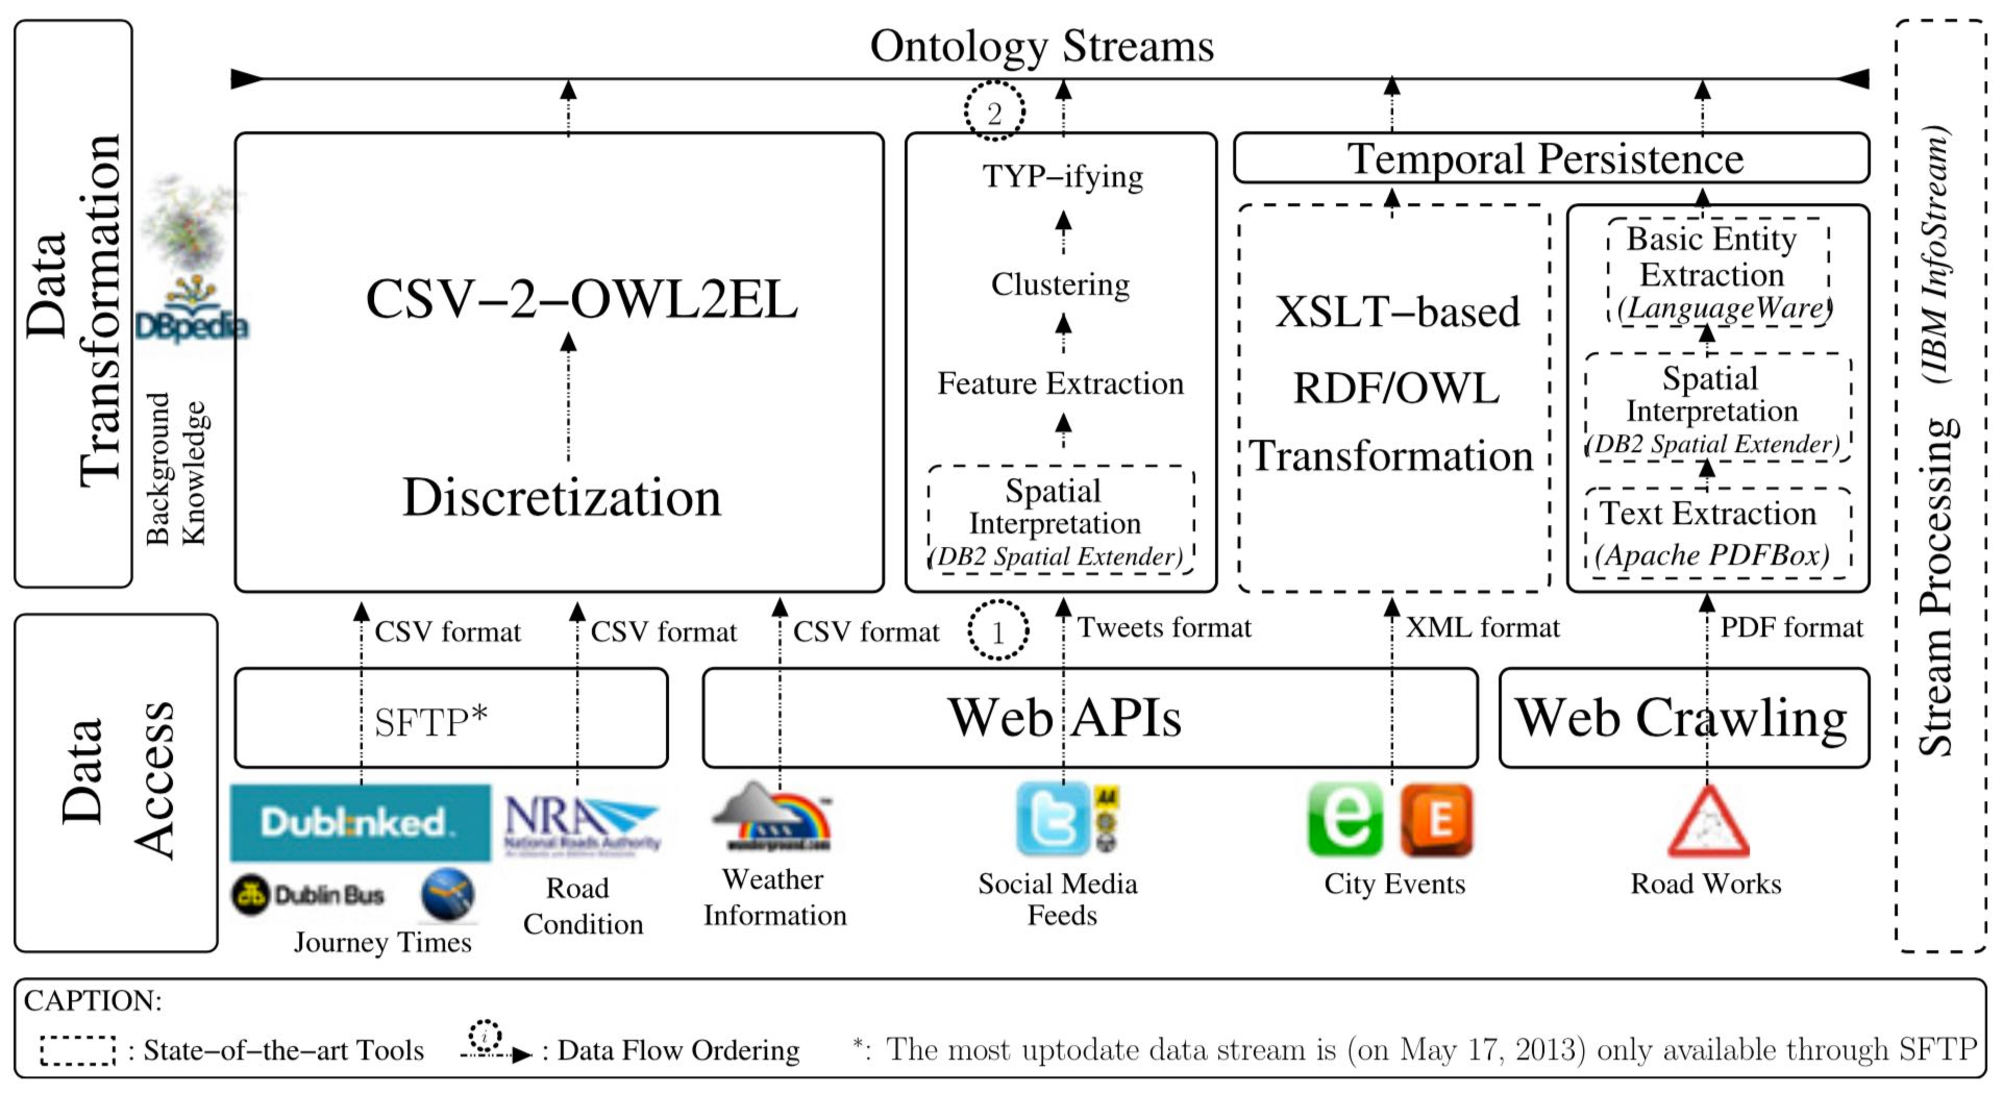
\includegraphics[width=0.75\textwidth]{img/starcity}.
    \caption{The STAR-CITY semantic stream enrichment (source~\cite{DBLP:journals/ws/LecueTHTBST14}).}
    \label{fig:star-city}
\end{figure}

The next sections present four different solutions for urban data analysis based on Semantic Web technologies.
Section~\ref{sec:uda-starcity} and Section~\ref{sec:uda-trafficlark} present respectively STAR-CITY and Traffic LarKC, two works that face the problem, from architectural point of view. Both of the presented solutions perform \textit{spatial} and \textit{temporal} analysis on the collected data to offer the best route to the user based on weather, traffic and other multiple external sources.
In Section~\ref{sec:uda-london} we propose an overview of the infrastructure we created for monitoring crowds movement during the 2012 Olympic Games in London. The solution exploits data from social network and perform \textit{content}, \textit{spatial} and \textit{temporal} analysis to spot emerging pattern and mobility dynamics and enables the creation of complex data visualizations.
Finally, Section~\ref{sec:uda-bottari} presents BOTTARI, a mobile application that performs \textit{content}, \textit{spatial} and \textit{temporal} analysis on social network and urban data to recommend restaurants to the user.

\subsection{Monitoring Traffic Using Semantic and Stream Technologies} \label{sec:uda-starcity}

In recent years, public administrations and governments are embracing Open Data in the attempt to made available information to increase transparency and improve accountability of public services. Many cities are offering data regarding transportation, environment, energy and planning. Web sources offer an abundance of information (e.g., ~weather information, bike sharing usage, etc.) and non-public data can also be accessed (e.g., current location and state of public transportation, CCTV images, etc.).
Lecue et al.\cite{DBLP:journals/ws/LecueTHTBST14} proposes Semantic Traffic Analytics and Reasoning for CITY (STAR-CITY), a solution designed to ease the integration of data characterized by variety (structured and unstructured), velocity (static and real time streaming data) and volume (large amount of historical data).

STAR-CITY exploits the W3C Semantic Web stack to represent the semantics of information and to elaborate the outcomes through a combination of reasoning techniques (Figure~\ref{fig:star-city} shows STAR-CITY semantic stream enrichment architecture). The solution was mainly designed to perform \textit{spatial} and \textit{temporal} analysis on heterogeneous data, on order to provide insights on historical and real-time traffic conditions.
The traffic scenario was chosen because most of the industrial countries are suffering of traffic congestion and transportation issues that can reduce the health of citizenship and can interfere with the passage of emergency vehicles.
The system was successfully tested in various scenario involving different cities (Dublin, Bologna, Miami and Rio).

\subsection{Semantic Traffic-Aware Routing} \label{sec:uda-trafficlark}

\begin{figure}[t]
	\centering
	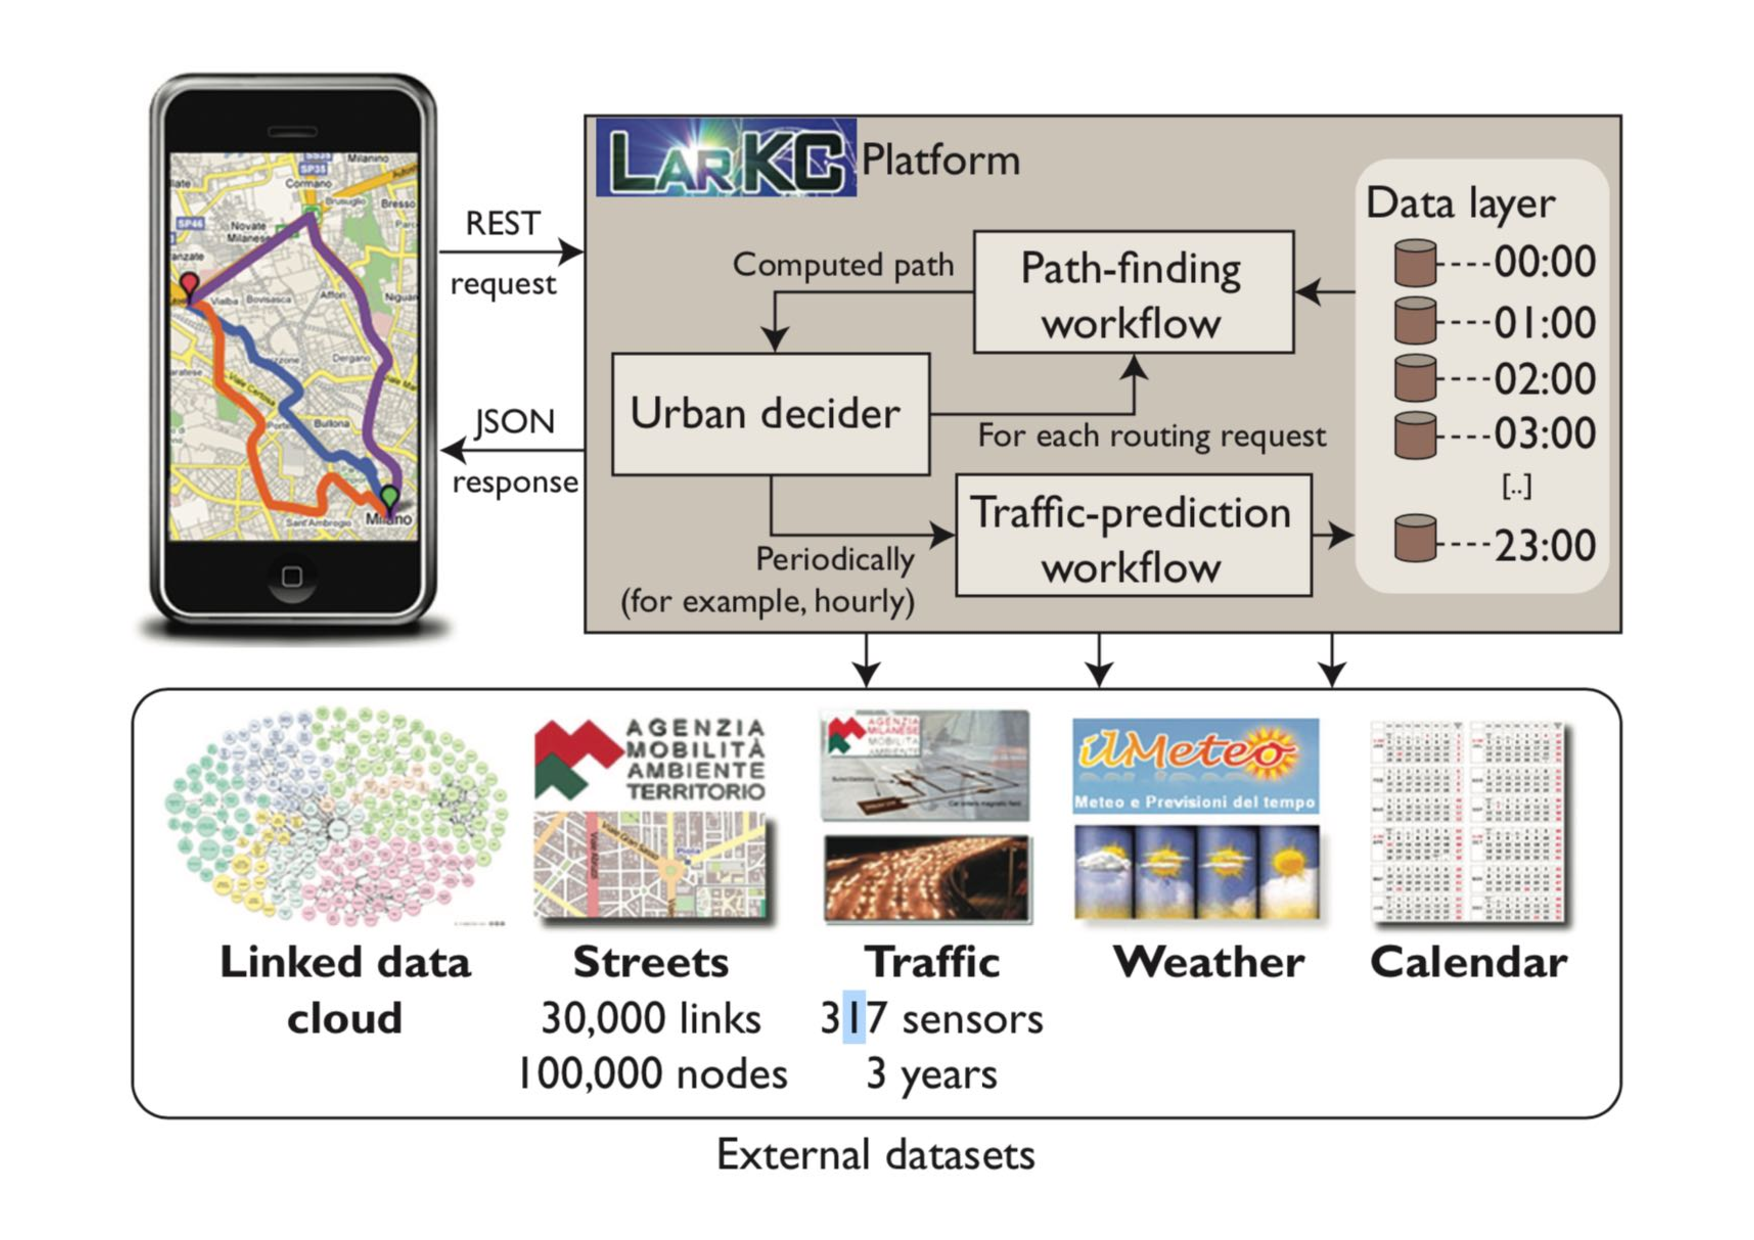
\includegraphics[width=0.75\textwidth]{img/traffic-lark.pdf}.
    \caption{The Traffic LarKC workflows and external datasets (source~\cite{DBLP:journals/internet/ValleCDGST11}).}
    \label{fig:traffic-lark}
\end{figure}

In the late 2000s, the increasing usage of mobile technologies to get directions and information about the surrounding presented various challenges. Those challenges were only partially solved by the existing research: operation research solved the routing problem, machine learning addressed traffic forecasting, and semantic technologies managed data integration and information retrieval. Therefore, the research of location-based comprehensive solution was still an open problem.

Traffic LarKC~\cite{DBLP:journals/internet/ValleCDGST11} is a fist attempt to build a comprehensive system able to tame of those challenges simultaneously.
It offers a mix of conceptual query answering, machine learning, and operations research.
It can answer questions like "What Asian restaurant can I reach in less than 15 minutes if I get into my car at 6 p.m.?". 

Figure \ref{fig:traffic-lark} depicts the Traffic LarKC workflows. The service exploits the LarkC platform\cite{DBLP:conf/semco/FenselHABCVFHKLSTWWZ08} to offer a comprehensive solution to periodically perform \textit{spatial} and \textit{temporal} analysis on the data and compute the best route taking in account weather, traffic and other data from external dataset.

\subsection{Monitoring Crowd Movement During London 2012 Olympics Games} \label{sec:uda-london}

\begin{figure}[t]
\centering
\subfloat[]{
	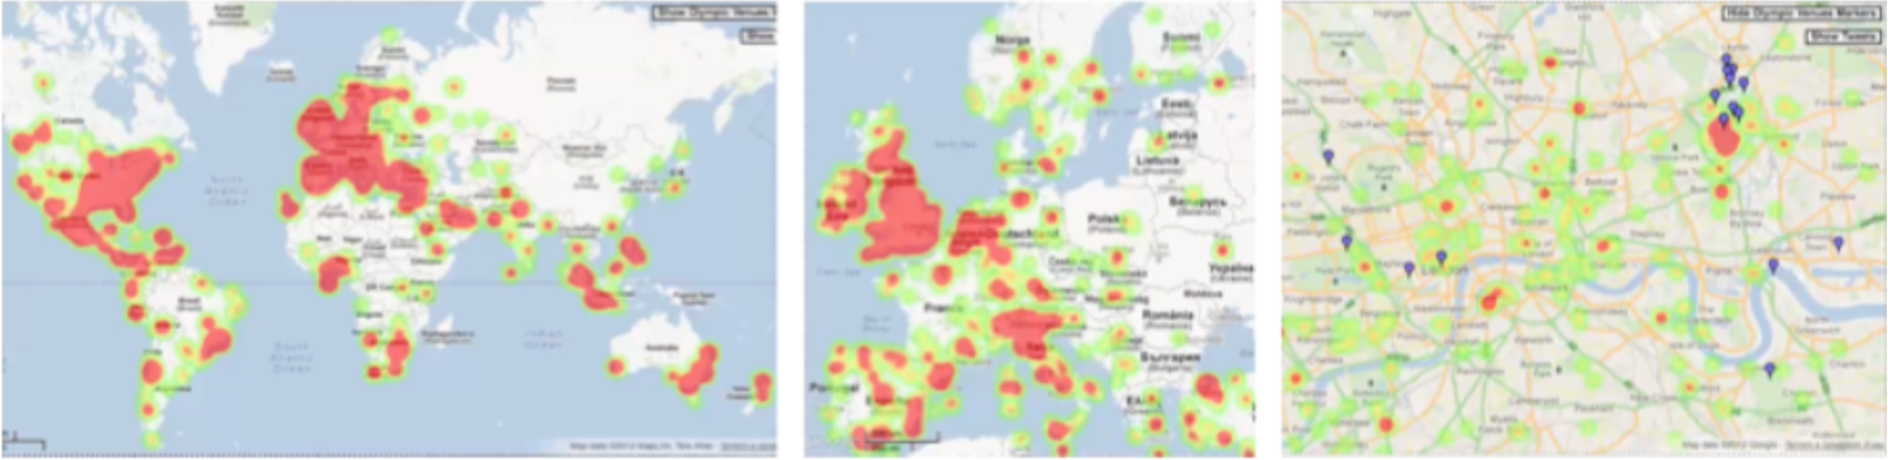
\includegraphics[width=0.8\textwidth]{img/london1}
} \\ 
\subfloat[]{
	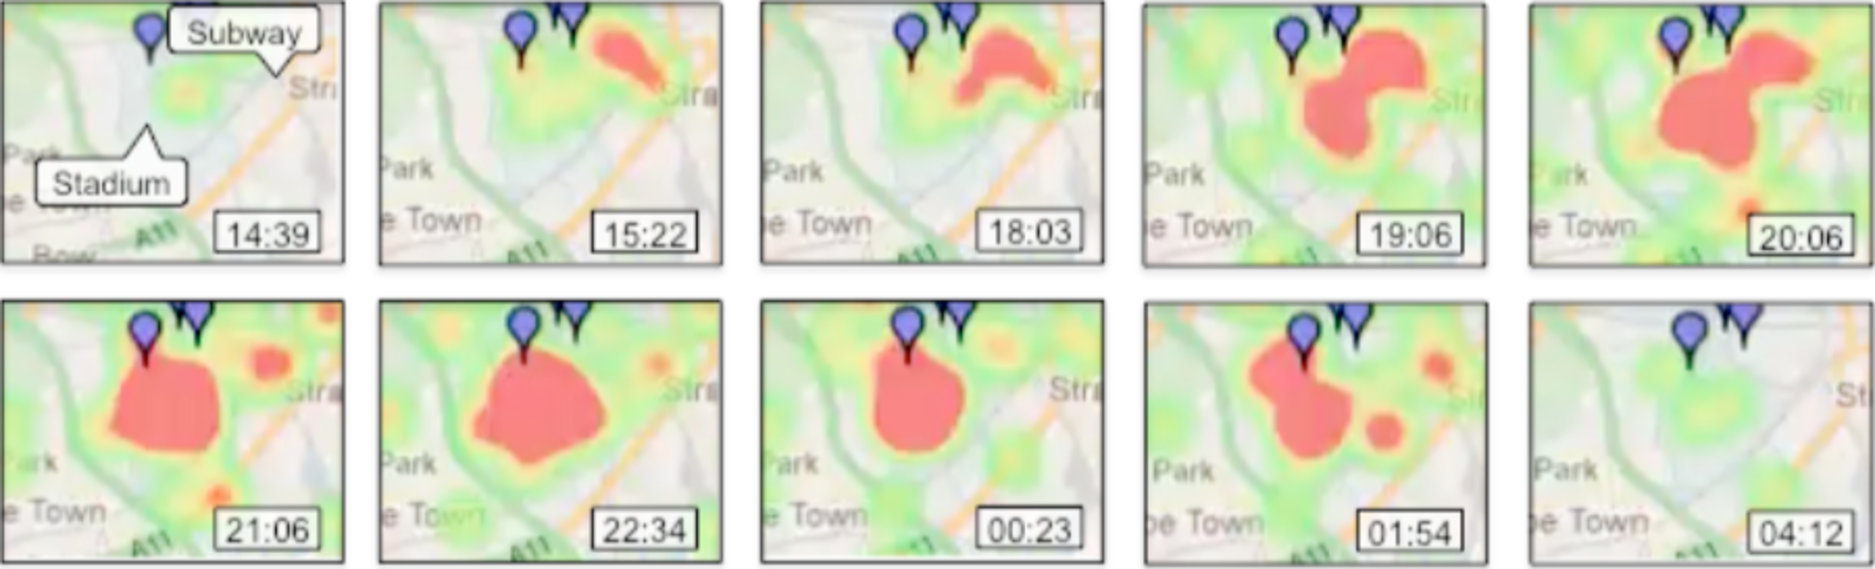
\includegraphics[width=0.8\textwidth]{img/london2}
}
\caption{The Figure (a) shows the people's interest at different zoom level during the Open ceremony of Olympic Games. Figure (b) shows the movement of the crowd in the surrounding of the Olympic Stadium at different time around the ceremony (source~\cite{DBLP:conf/semweb/BalduiniVDTPC13}).}
\label{fig:london-move}
\end{figure}

The work presented in this section shows how to track the movements of the crowds in big events exploiting the analysis of geo-tagged tweets.
Previous work shows that the data from social network is incomplete and inconsistent (see Section~\ref{sec:vel-var-solutions}) and the proposed system must deal with these data characteristics.

The presented system exploits the C-SPARQL Engine~\cite{DBLP:journals/ijsc/BarbieriBCVG10} within SLD (see Section~\ref{sec:sld}) framework in order to perform \textit{content}, \textit{spatial} and \textit{temporal} analysis on Social Media streams (i.e., Twitter). 
It models the data in a convenient format and exploits OBDA to extract the position on the interesting geo-tagged tweets. 
Being public not only the position of the tweet but also the content, the system can track the people attention and select only the tweets with content related to the event. 

Figure~\ref{fig:london-move}(a) shows the attention of the people at different space granularity, i.e. World, Europe, City of London, during the London 2012 Open Ceremony. The information was extracted from Tweets selected exploiting keywords present in text of the content.
Figure~\ref{fig:london-move}(b) shows movements of the crowd before, during and after the Olympics open ceremony. Exploiting the Tweets position the system can clearly shows people arriving at the Olympic Stadium, entering the Olympic Stadium and leaving the Olympic Stadium.
Figure~\ref{fig:london-move}(a) and Figure~\ref{fig:london-move}(b) shows how the infrastructure can enable visual analytics. 
Both of the figure are based on the same data, but, while the former enables the observation of world-wide attention pattern, the latter offers insights of crowds' movements in a given area.

\subsection{Bottari} \label{sec:uda-bottari}

\begin{figure}[t]
	\centering
	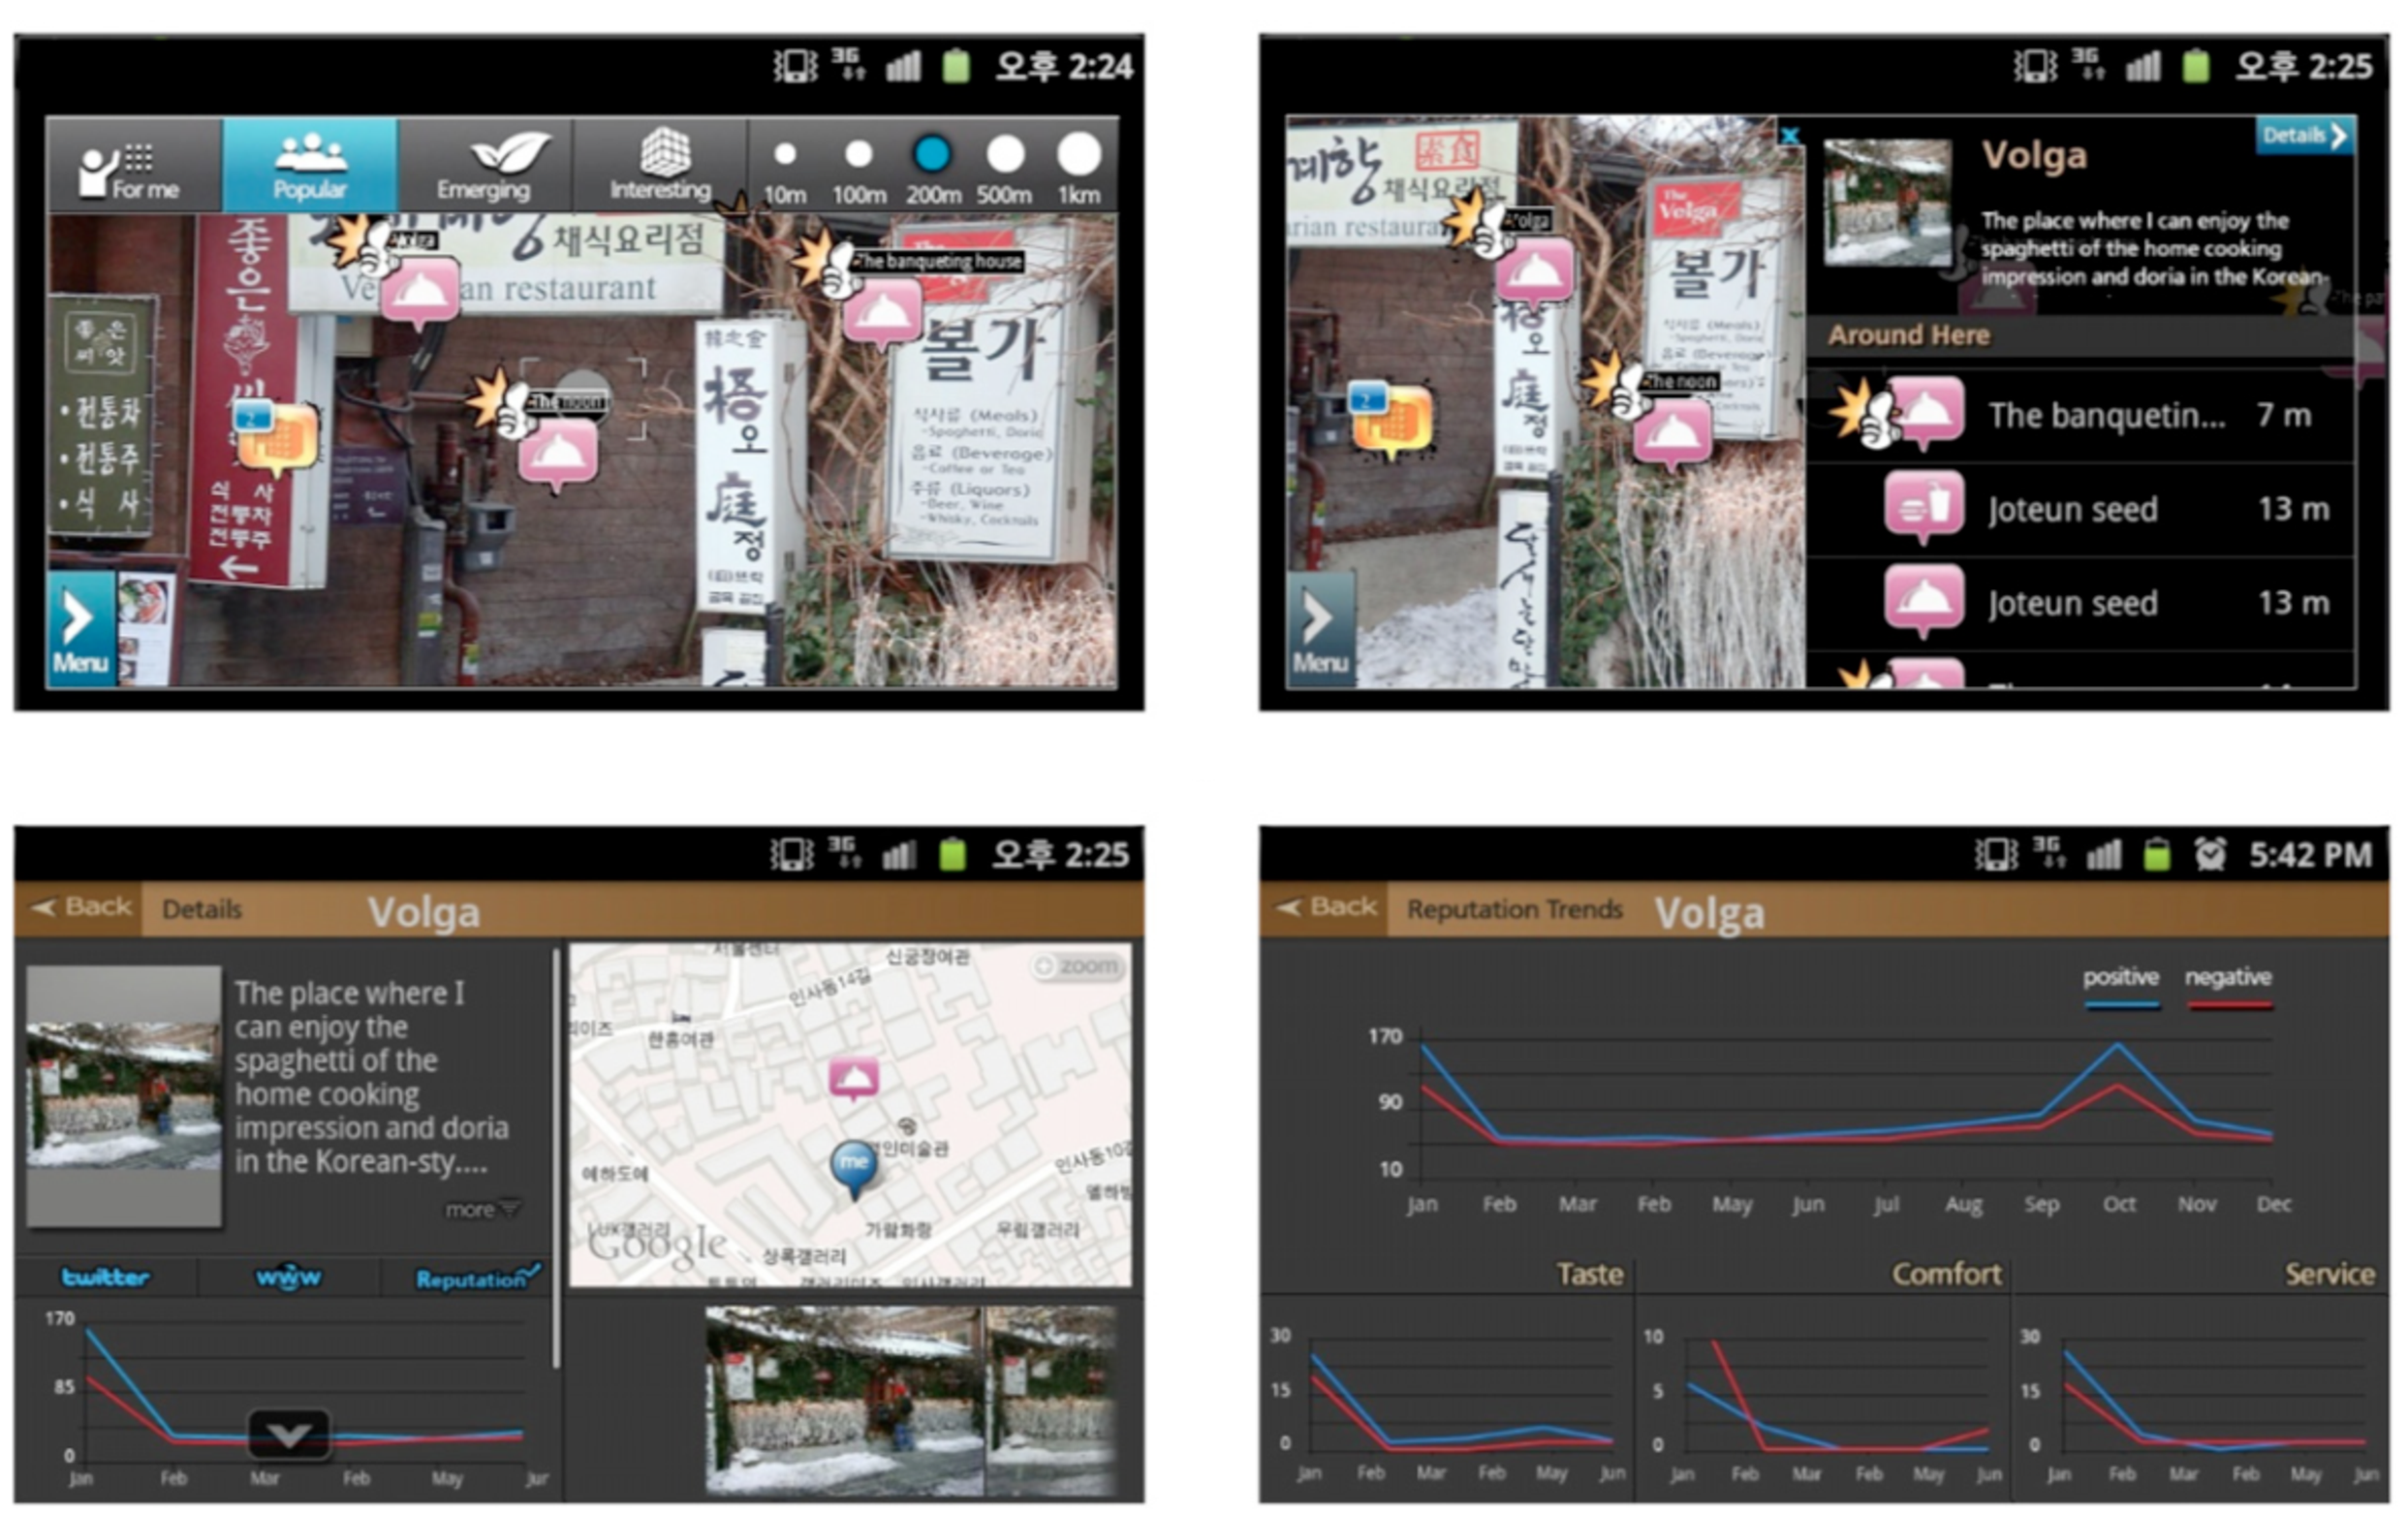
\includegraphics[width=0.75\textwidth]{img/bottari2.pdf}.
    \caption{BOTTARI visualizations (source~\cite{DBLP:conf/semweb/BalduiniVDTPC13}).}
    \label{fig:bottari-vis}
\end{figure}

In 2011, an average of three million tweets per day was posted in Seoul and many of that carry the user's live opinion about restaurants, bars, cafes, and many other semi-public points of interest (POIs) in the city. 
The stream of data, which we continuously collected, results (i) incomplete, i.e. only 41\% of users rated at least the same POI, and (ii) inconsistent, i.e. many users rates a POI several times in different way.
BOTTARI~\cite{DBLP:journals/ws/BalduiniCDVHLKT12} exploits inductive and deductive stream reasoning (see Section \ref{sec:sr-rsp}) to continuously perform \textit{content}, \textit{spatial} and \textit{temporal} analysis on Social Media streams (i.e., Twitter) in order to understand how the Social Media users collectively perceive the POIs in a given area (e.g., Insadong's restaurants) and build a recommendation engine.

BOTTARI is designed following an OBDI architecture (see Section \ref{sec:obdi-obda}). 
The infrastructure behind BOTTARI application is pluggable and is based on SLD framework (see Section \ref{sec:sld}). 
A first component in SLD pipeline casts in RDF the data item in the stream. 
A second downstream component performs the analysis exploiting the C-SPARQL Engine (see Section \ref{sec:vel-var-solutions}) as deductive stream reasoner
A last downstream component, based on the Statistical Unit Node Set (SUNS) \cite{tresp2009materializing,huang2010multivariate} approach, acts as inductive stream reasoner.
The data was continuously collected and modeled using BOTTARI ontology, an extension of SIOC vocabulary, to cope with the variety.

Figure~\ref{fig:bottari-vis} shows the various visualization offered by the augmented reality Android application that returns BOTTARI results to the end user. Such an application guides the user to the POI choice. The presented POIs are based on the deductive/inductive stream reasoning results and are personalized for the user. 
%Conceptual Model
\chapter{Conceptual Model}\label{ch:conceptual}

In this chapter, we propose a conceptual model named \frappe{}~\cite{DBLP:conf/semweb/BalduiniV15}. \frappe{} is a vocabulary that bridge the gap between the data engineer and visual interface designers for enabling visual analytics for the detection, the understanding and the interpretation of spatio-temporal data.
We introduce the problem, solved by \frappe{}, in Section~\ref{sec:conc-intro}.
In Section~\ref{sec:conc-fr-1}, we present an overview of the first version of \frappe{}.
In Section~\ref{sec:conc-fr-2}, we propose \frappe{} 2.0, an extension of the original vocabulary where we expand the provenance fragment and add a content related fragment.
Finally, Section~\ref{sec:conc-fr-2-analysis} presents an overview of the analysis enabled by \frappe{} 2.0.

\section{Introduction and Problem Statement}\label{sec:conc-intro}
Since the last decade, the rapid increase of sources, which expose geo-located time-varying data, has been drawing attention of those who are looking for data-driven decision making. 
The availability of social media, telecommunication, traffic and weather data improved the ability to capture peoples' interests, habits and preferences.

In particular, the growing availability of urban data sources (see Chapter~\ref{ch:uda}) stimulated the research of a holistic conceptual model to manage data variety in a comprehensive way. The current interest is for solutions that enable the fusion of streaming heterogeneous data to enable reactive decisions.

One of the main assumptions of any smart-city approach is to work upon a layer of data collected from the city itself that describes its dynamics. The city evolution can span multiple layers, from architecture to urban design, from population composition and migrations to citizen behaviors and interests. Each of these layers has a different dynamics and speed of change.
Therefore, it should be monitored collecting data from different sources and using multiple analysis techniques (see Section~\ref{sec:uda-analysis}). 

\begin{figure}[t]
\centering
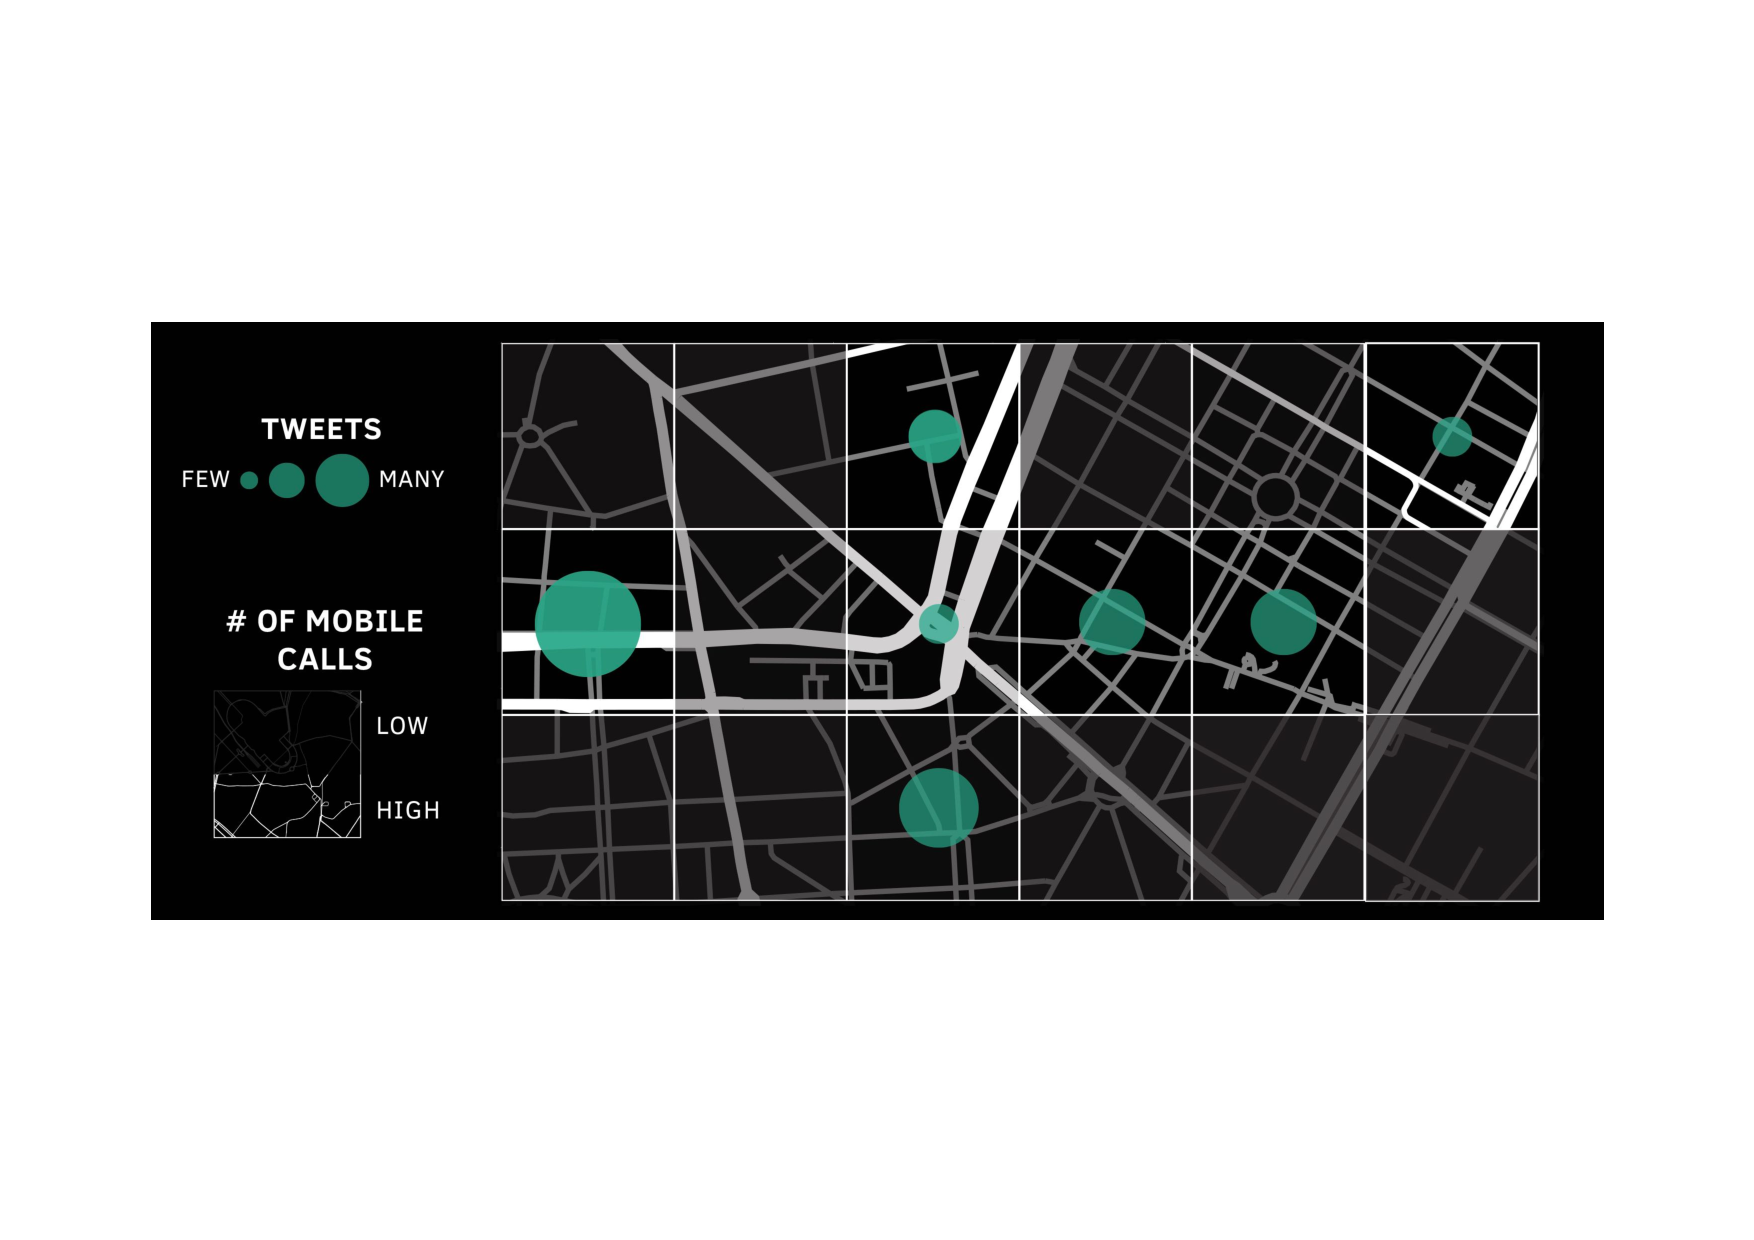
\includegraphics[width=0.8\textwidth]{img/real-world-rep}
\caption{A real-world example of visual analytics of two heterogeneous datasets. (source~\cite{DBLP:conf/semweb/BalduiniV15}).}
\label{fig:real-world-rep}
\end{figure} 

In particular, our research question, presented in Section~\ref{sec:prob_rq}, refers to visual analytics\footnote{The science of analytical reasoning facilitated by interactive visual interfaces~\cite{cook2005illuminating}.} as a way for making sense of heterogeneous spatio-temporal streaming data.
For instance, Figure~\ref{fig:real-world-rep} illustrates a real case of visual analytics for a general audience we experimented during the Milano Design Week events (see Section~\ref{sec:cs-mdw-2014}).
The Figure presents a grid of 6x3 cells overlaid to a city street map. Green circles can appear in each cell. They visually represent the number of tweets posted in a time interval from each cell. The fill color opacity value of each cell is, instead, mapped to the number of mobile calls from each cell. As we showed in Section~\ref{sec:cs-mdw-2014}, people without specific expertise in data analytics can easily guess the cells where the two signals are correlated.

Unfortunately, data is not often ready for visual analytics.
A gap exists between the terms used by the designers who create the visual analytics interface and those used by the computer scientists who prepare the data. The designers expect data aggregated over time and space, while the data engineers talk about fine-grained geo-located time-varying data.
For instance, in 2012, during the BOTTARI experiment (see Section~\ref{sec:uda-bottari}) in the city of Seoul, we model data using SMA ontology (see Figure~\ref{fig:sma-onto}).
SMA extends the SIOC vocabulary\footnote{\url{http://sioc-project.org/}} adding the spatial aspect. To do so, it exploits terms from W3C WGS-84 vocabulary\footnote{\url{https://www.w3.org/2003/01/geo/}}.
SMA poses the attention only on the raw data representation.
It does not include any specific concept to represent data aggregations or data abstractions to enable advanced analytics, which is one of the goal of this thesis.

\begin{figure}[t]
\centering
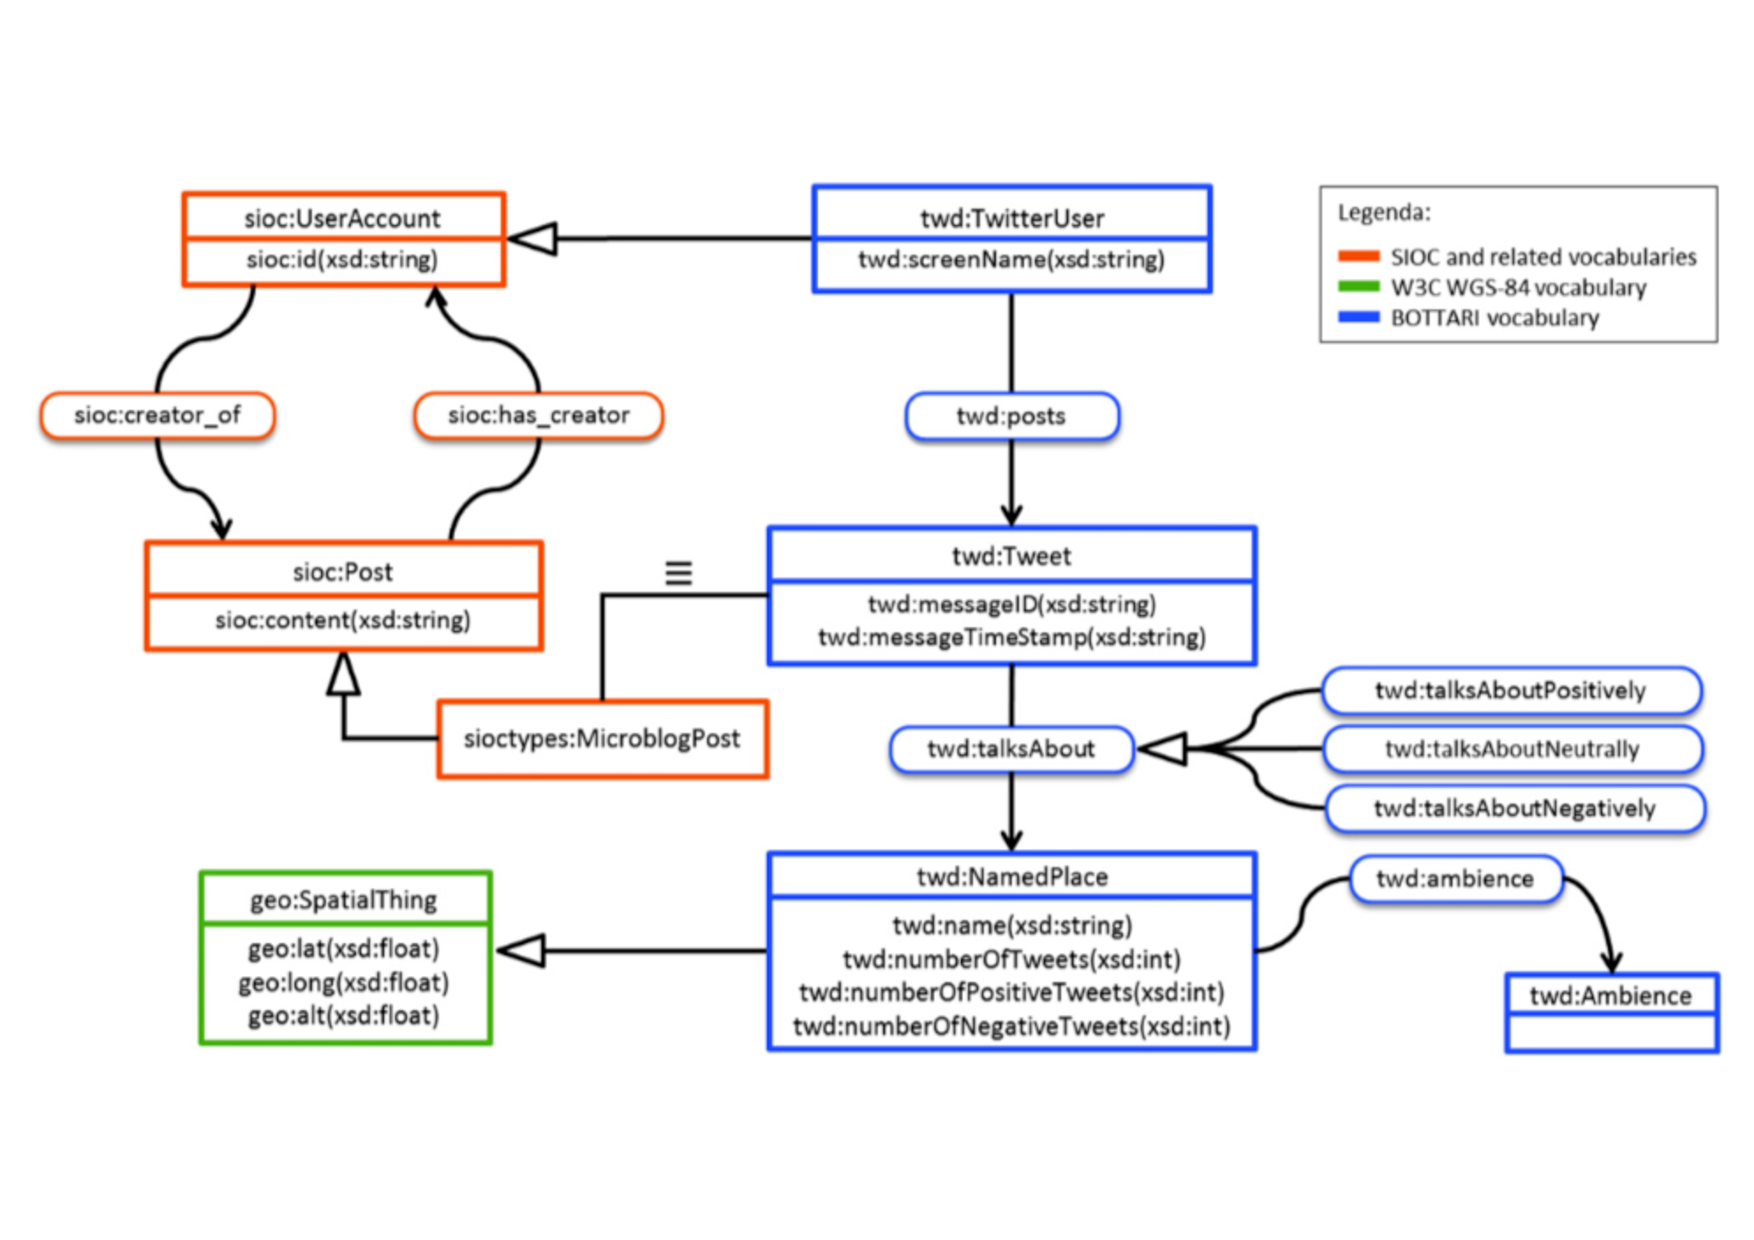
\includegraphics[width=0.85\textwidth]{img/sma-ontology}
\caption{Overview of the SMA ontology used in the BOTTARI project to model the data (source \cite{DBLP:journals/ws/BalduiniCDVHLKT12}).}
\label{fig:sma-onto}
\end{figure}

During years of collaboration with the Design Department of Politecnico di Milano\footnote{\url{https://densitydesign.org/}}, we discover that image processing terms like \textsf{Pixel} or \textsf{Frame} are common among both designers and data engineers. They represent a bridge between who prepare the data and who create the interfaces for visualizing it.

With this observation in mind, in order to answer the research questions, we formulated the hypotheses \textsf{Hp.1.1} and \textsf{Hp.1.2}

\begin{itemize}[leftmargin=42pt]
\item[\textsf{Hp.1.1}] A conceptual model containing terms from the image processing domain can represent spatio-temporal data in an extendable and coherent way with a minimal encoding bias and a minimal ontological commitment.
\item[\textsf{Hp.1.2}] Visual analytics interfaces built directly on data represented with the conceptual model of Hp.1.1 are guessable\footnote{The guessability is defined as the measure of the cost to the user involved in using an interface to perform a new task for the first time. The lower the cost, the higher the guessability~\cite{moyes1993icon}. The cost can be measured in terms of time, errors, or effort.}.
\end{itemize}

\section{\frappe{} 1.0}\label{sec:conc-fr-1}
In this section, we propose our first attempt to create a conceptual model to represent spatio-temporal data.
Section~\ref{sec:conc-fr-1-mod} exposes the main concepts behind \frappe{} and the development methodology.
In Section~\ref{sec:conc-fr-1-eval}, we present an evaluation of \frappe{} 1.0 based on its adherence to the Tom Gruber's  principles~\cite{DBLP:journals/ijmms/Gruber95}.
Finally, Section~\ref{sec:conc-fr-1-synth-ex} presents a working example, where we use \frappe{} 1.0 to model the data of the DEBS Grand Challenge 2015\footnote{\url{http://www.debs2015.org/call-grand-challenge.html}}.

\subsection{The Conceptual Model}\label{sec:conc-fr-1-mod}
In order to verify the hypotheses \textsf{Hp.1.1} and \textsf{Hp.1.2}, we proposed the conceptual model \frappe{}. It is named out of its four main concepts: Frame, Pixel, Place and Event.
In this section, we refer to \frappe{} 1.0 as \frappe{}.

\begin{figure}[t]
\centering
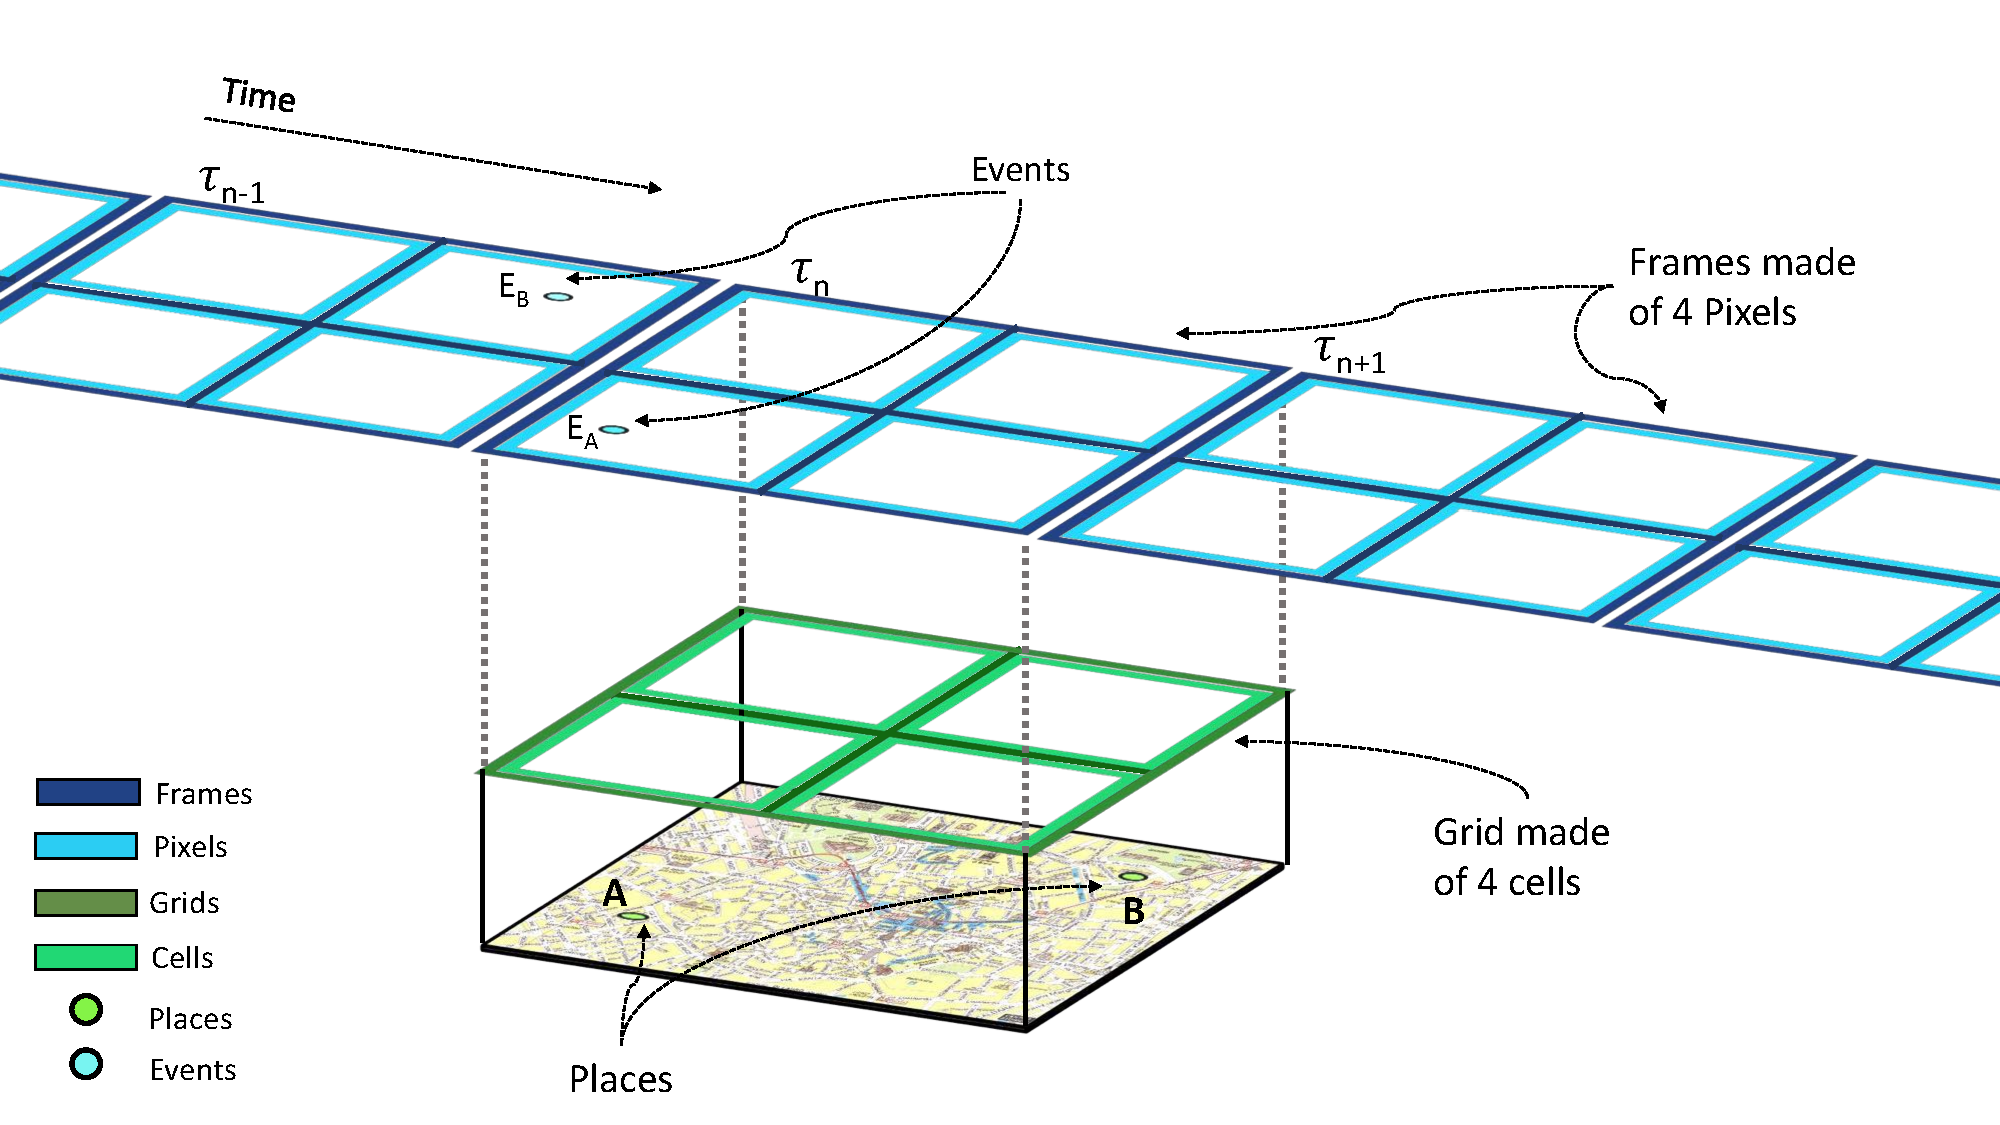
\includegraphics[width=0.8\textwidth]{img/conceptual-model-overview}
\caption{A high-level view of \frappe{} including 3 \textsf{Frame}s made of
4 \textsf{Pixel}s containing the \textsf{Place}s where the \textsf{Event}s happen.}
\label{fig:overview}
\end{figure}

\frappe{} ontology is formalized using the version 2 of the Web Ontology Language (see Section~\ref{sec:owl}). It reuses GeoSparql~\cite{battle2011geosparql} as geographical data model, the Time~\cite{Hobbs2006} and Event ontologies~\cite{RaimondAbdallahEventOntology2007}) as time/event vocabularies, and PROV-~O~\cite{w3c-prov-o} as provenance ontology. 

\frappe{} enables an OBDA approach for the data analysis by exploiting the terms imported from GeoSparql, Time, Event and PROV-O ontologies without any axiomatization. This is because OBDA requires OWL2-QL ontologies, while \frappe{} with the imported ontologies is in OWL2 Full. 

\frappe{} offers a high level view of the detection, the understanding, and the interpretation of geo-spatial time-varying data.
It uses a digital image processing metaphor (see Figure \ref{fig:overview}) to track the three main dimensions of analysis introduced in Section~\ref{sec:uda-analysis}: space, time, and content. 

\frappe{} assumes that the real world can be described as a bi-dimensional space, where \textsf{Event}s happen in \textsf{Place}s over time. For instance, a user making a check-in on a geo-located social network generates an event in a place. A taxi ride generates a sequence of two events (a pick-up and a drop-off) in two distinct places. A garbage collector truck generates a sequence of events around the city in different points in time, one for each trash bin it cleans up.

\begin{figure}[t]
\centering
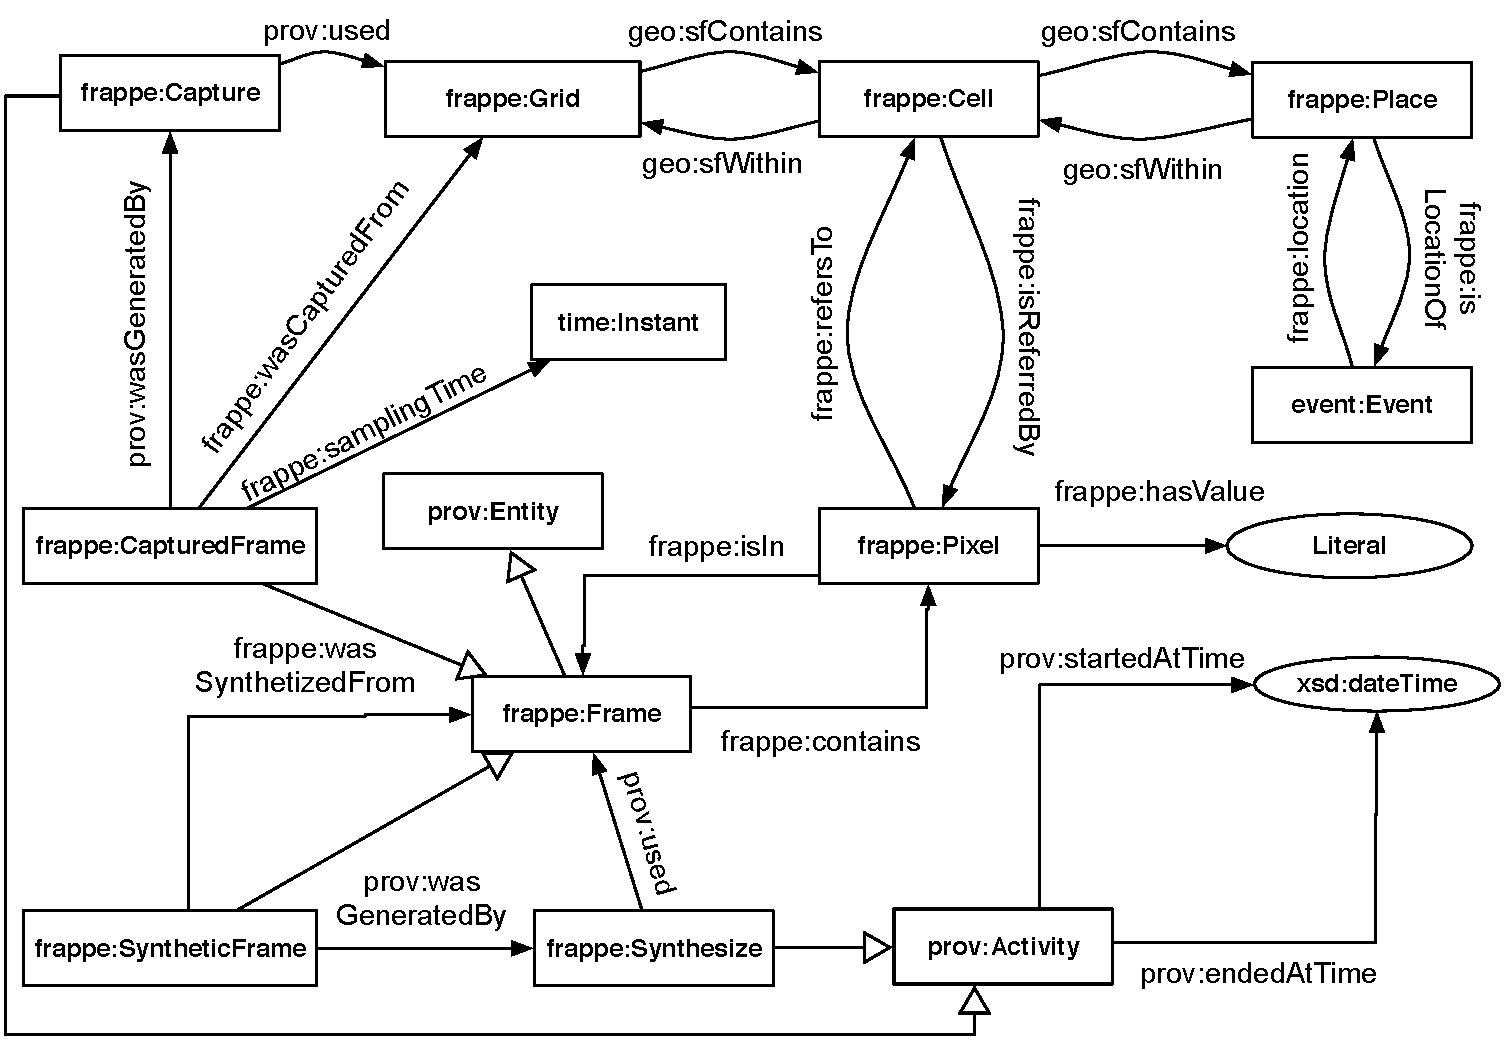
\includegraphics[width=0.85\textwidth]{img/conceptual-model-original-core}
\caption{The UML representation of the original version of the \frappe{} ontology}
\label{fig:original-core}
\end{figure} 

Figure~\ref{fig:original-core} depicts all the main concepts in the model.
\frappe{} is organized in three interconnected parts: the geographical, the time-varying and the provenance fragments.
It proposes to capture the digital footprints of what happens in the real-world as a sequence of \textsf{Frame}s. A \textsf{Grid} sits between the physical world and the frames of the film. It decomposes the physical world in \textsf{Cell}s. Each frame is, therefore, decomposed accordingly in \textsf{Pixel}s.

More formally, \textsf{Place}, \textsf{Cell} and \textsf{Grid} belong to the geographical fragment and reuse terms from the GeoSparql vocabulary~\cite{battle2011geosparql}. 
%They are geosparql \texttt{Feature}s whose default geometry are respectively a \texttt{point}, a \texttt{surface} and a \texttt{multisurface}. 
\textsf{Event}, \textsf{Pixel} and \textsf{Frame} are in the time-varying part. The \textsf{Event} term is borrowed from the Event ontology~\cite{RaimondAbdallahEventOntology2007}. 
The provenance part includes the activities \textsf{Capture} and \textsf{Synthesize} and reuses the PROV Ontology~\cite{w3c-prov-o} (PROV-O).

An \textsf{Event} has a \textsf{location} in a \textsf{Place} in a \textsf{Cell} -- the basic spatial unit of aggregation of information in \frappe{} -- which, in turn, is in a \textsf{Grid}.

A \textsf{Pixel} is the time-varying representation of a \textsf{Cell}. It is the only element in \frappe{} 1.0 that carries information through the \textsf{hasValue} data property. As in image processing, this value represents a measure of intensity of some phenomenon in the real world. For instance, it can represent the number of micro-posts posted in a given time interval in a certain \textsf{Cell}. Each \textsf{Pixel} \textsf{refersTo} a single \textsf{Cell}, contrariwise a \textsf{Cell} could be \textsf{referredBy} many different \textsf{Pixel}s that captures different information associated to the same \textsf{Cell}, e.g., the already mentioned number of micro-posts, but also the number of mobile phone calls or the number of goods' pick-ups.

Similarly, a \textsf{Frame} is the time-varying counterpart of a \textsf{Grid} and a sequence of \textsf{Frame}s composes the film of the evolution of a physical portion of the world over time. 
\frappe{} distinguishes between two specializations of \textsf{Frame}s: the \textsf{CapturedFrame}s and the \textsf{SyntheticFrame}s. 
\textsf{Frame} and \textsf{Grid} are \textit{Entity} in PROV-O. This is because \frappe{} proposes the ternary relationships \textsf{Capture} and \textsf{Synthesize} as specializations of the relationship \textit{Activity} of PROV-O.

A \textsf{CapturedFrame} \textit{wasGeneratedBy} a \textsf{Capture} \textit{Activity} \textit{startedAtTime} $\tau_i$ and \textit{endedAtTime} $\tau_j$ that \textit{used} a given \textsf{Grid}. It \textsf{contains} a \textsf{Pixel} for every \textsf{Cell} in the \textsf{Grid} it \textsf{wasCapturedFrom}. Different \textsf{Frame}s represent different images of the observed phenomena at the same \textsf{samplingTime} (e.g., a frame captured the volume of the social activity while another one captured the volume of the mobile phone calls at 12.00).
The object property \textsf{wasCapturedFrom} is the result of the chaining of the two \textit{wasGeneratedBy} and \textit{used} object properties. Moreover, the value of the \textsf{samplingTime} data property, which describes the \textsf{CapturedFrame}, is the one assigned to the \textit{startedAtTime} data property that describes the captured activity. 

Similarly, a \textsf{SyntheticFrame} \textit{wasGeneratedBy} by a \textsf{Synthesize} \textit{Activity} that \textit{used} one or more \textsf{Frame}s. The idea is to derive a \textsf{Frame} from one or more others. The \textsf{Synthesize} operation can be a filter applied to the values of the pixels, or an aggregation of values of \textsf{Pixel}s across \textsf{Frame}s or the difference between the values associated to the \textsf{Pixel}s of two different \textsf{Frame}s. 

We develop \frappe{} using METHONTOLOGY~\cite{fernandez1997methontology} (see Section~\ref{sec:onto-eng}) methodology by following the whole ontology life cycle.
%specification
We started from the specification phase following, in the scoping activity, a middle-out approach (see Section~4.1 in~\cite{fernandez1997methontology}). We exploited terms from image processing and spatial glossaries in order to find the primary concepts of \frappe{} and to verify, at the earliest possible stage, the conciseness and completeness of our specification. 
%conceptualization
We then conceptualized the specification and produced a complete  Glossary of Terms (GT).
%integration
Most of the concepts in \frappe{} are directly integrated from other domain specific ontologies (e.g., Instant from Time ontology~\cite{Hobbs2006}, Activity from PROV-O ontology~\cite{w3c-prov-o}, etc.)
%Evaluation

\subsection{Adherence to the Tom Gruber's Principles} \label{sec:conc-fr-1-eval}
We evaluated \frappe{}, by checking if it adhere the five principles of Tom Gruber~\cite{DBLP:journals/ijmms/Gruber95}: 
clarity, coherence, minimal encoding bias, minimal ontological commitment and extendibility.

\frappe{} satisfies the \textit{clarity} principle because all definitions are documented in natural language (see the version of \frappe{} published on github\footnote{\url{https://github.com/streamreasoning/FraPPE.git}}). The terms proposed in \frappe{} are: (i) common terms in spatial-related vocabularies (e.g., \textsf{Place}, \textsf{Cell}, \textsf{Grid}); (ii) well known terms of the image processing domain (e.g., \textsf{Pixel}, \textsf{Frame}, \textsf{Capture}, or \textsf{Synthesize}); and (iii) terms defined in other ontologies (e.g., Event, Instant, Entity, or Activity). 

\frappe{} has a \textit{minimal encoding bias} because it is encoded in OWL2. Moreover, we explicitly avoided adding cardinality restrictions, because, in our works (see Chapter~\ref{ch:case-studies}), we use \frappe{} to integrate data following an Ontology-Based Data Access approach which requires OWL2 profile that does not include cardinality restrictions.   

\frappe{} requires a \textit{minimal ontological commitment}, meaning that, as Tom Gruber recommended, \frappe{} makes as few claims as possible about the geo-located time-varying data being modeled allowing who uses \frappe{} to specialize and instantiate it as needed.

We tested in details that \frappe{} is \textit{extendable} by successfully modeling the dataset made available by ACM DEBS 2015 Grand Challenge\footnote{\url{http://www.debs2015.org/call-grand-challenge.html}}, for all the details, see Section~\ref{sec:conc-fr-1-synth-ex}.
Moreover, we check the extendibility of \frappe{} while using it in the experiences reported in the Chapter~\ref{ch:case-studies}. For further details see Section~\ref{sec:cs-conclusion}.

Last but not least, \frappe{} is \textit{coherent}, i.e., all \frappe{} inferences at T-box level are consistent with the definitions and in modeling A-boxes containing social, telecommunication, environment, traffic, and energy consumption data, we never inferred inconsistent or meaningless data.

\begin{figure}[p]
\begin{minipage}{0.95\linewidth}
\begin{lstlisting}[label={lst:debs}, caption={Fraction of the model representing ACM DEBS Grand Challenge 2015 Data}, style=N3]
@prefix frGrid: <http://streamreasoning.org/debsGC/Grids/> .
@prefix frCell: <http://streamreasoning.org/debsGC/Cells/> .
@prefix frPixel: <http://streamreasoning.org/debsGC/Pixels/> .
@prefix frPlace: http://streamreasoning.org/debsGC/Places/:> .
@prefix frEvent: <http://streamreasoning.org/debsGC/Events/> .
@prefix frFrame: <http://streamreasoning.org/debsGC/Frames/> .
@prefix frCapture: <http://streamreasoning.org/debsGC/Captures/> .

frGrid:Grid_1 gs:sfContains frCell:Cell_1, frCell:Cell_2 .

frCell:Cell_1 a fr:Cell ;
    rdfs:label "39460"^^xsd:long ;
    fr:isReferredBy frPixel:1356995100000_39460 ;
    gs:sfContains frPlace:A ;
    gs:sfWithin frGrid:Grid_1 .

frPlace:A a sf:Point ;
    fr:isLocationOf frEvent:E_B ;
    gs:asWKT "POINT( 40.715008 -73.96244 )"^^gs:wktLiteral ;
    gs:sfWithin frCell:Cell_1 .

frEvent:E_A a fr4d:PickUpEvent ; 
    a event:Event ;
    event:time [ a time:Instant ; 
       time:inXSDDateTime "2013-01-01T00:00:00"^^xsd:dateTime ] ;
    fr:location frPlace:A> ;
    fr4d:hackLicense "E7750A37CAB07D0DFF0AF7E3573AC141"^^xsd:string ;
    fr4d:medallion "07290D3599E7A0D62097A346EFCC1FB5"^^xsd:string .

frEvent:E_B a fr4d:DropOffEvent ; 
    a event:Event ;
    event:time [ a time:Instant ; 
       time:inXSDDateTime "2013-01-01T00:02:00"^^xsd:dateTime ] ;
    fr:location frPlace:B ;
    fr4d:connected frEvent:E_A ;
    fr4d:fareAmount "3.5"^^xsd:double ;
    fr4d:mtaTax "5.0"^^xsd:double ;
    fr4d:paymentType "CSH"^^xsd:string ;
    fr4d:surcharge "5.0"^^xsd:double ;
    fr4d:totalAmount "4.5"^^xsd:double ;
    fr4d:tripDistance "0.44"^^xsd:long ;
    fr4d:tripTime "120"^^xsd:long .

frPixel:1356995100000_39460 a fr:Pixel ;
    fr:isIn frFrame:1356995100000 ;
    fr:refers frCell:Cell_1 .

frFrame:1356995100000 a fr:CapturedFrame ;
    fr:contains frPixel:1356995100000_39460, 
    frPixel:1356995100000_39461 ;
    fr:samplingTime [ a time:Instant ; 
       time:inXSDDateTime "2013-01-01T00:05:00"^^xsd:dateTime ];
    fr:wasCapturedFrom frGrid:Grid_1 ;
    prov:wasGeneratedBy frCapture:1356995100000 .
\end{lstlisting}
\end{minipage}
\end{figure} 

\subsection{Working Example} \label{sec:conc-fr-1-synth-ex}

\begin{figure}[t]
\begin{minipage}[t]{0.95\linewidth}
\begin{lstlisting}[label={lst:sparql-debs}, caption={Sparql query to create the \textsc{SytheticFrame}s containing the \textsc{Pixel}s with the profitability value.}, style=SPARQL]
PREFIX   rdf:<http://www.w3.org/1999/02/22-rdf-syntax-ns#>
PREFIX   xsd:<http://www.w3.org/2001/XMLSchema#>
PREFIX   time:<http://www.w3.org/2006/time#>
PREFIX   f4d:<http://streamreasoning.org/ontologies/frappe4debs#>
PREFIX   prov:<http://www.w3.org/ns/prov#> 
PREFIX   event:<http://purl.org/NET/c4dm/event.owl#>
PREFIX   geos:<http://www.opengis.net/ont/geosparql#>
PREFIX   rdfs:<http://www.w3.org/2000/01/rdf-schema#>
PREFIX   fr:<http://streamreasoning.org/ontologies/frappe#>
PREFIX   sf:<http://www.opengis.net/ont/sf#>

CONSTRUCT{
    concat("frFrame:",now()") a fr:SyntheticFrame ;
    fr:contains ?pixel ;
    fr:samplingTime [ a time:Instant ; 
    		time:inXSDDateTime ?time ] ;
    fr:wasSynthesizedFrom ?frame . 
    ...
}
WHERE {
	?pixel f:isIn ?frame ;
	fr:refers ?cell .
	?cell geos:sfContains ?place ;
	rdfs:label ?cellLabel .
	?place f:isLocationOf ?e .
	?e a f4d:DropOffEvent ;
	f4d:totalAmount ?t .
	?frame time:hasBeginning ?beginning .
	?beginning time:inXSDDateTime ?time .
	FILTER(?time >= \"2013-01-01T00:10:00\"^^xsd:dateTime
    && ?time <= \"2013-01-01T00:15:00\"^^xsd:dateTime)"
}
GROUP BY ?pixel ?cell ?cellLabel
\end{lstlisting}
\end{minipage}
\end{figure} 

The ACM DEBS 2015 Grand Challenge proposes a taxi route analysis scenario based on a grid of 150x150 Kms with cells of 500x500 m. A stream of data represents the route of a taxi rides in terms of: (i) taxi description, (ii) pick-up and drop-off information (e.g., geographical coordinates of the place and time of the event), and (iii) ride information (e.g., tip, payment type and total amount).
In Listing~\ref{lst:debs}, we report a subset of the information representing a single taxi ride in \frappe{}. The pick-up \textsf{Event} represents the start of the ride and contains the taxi id. The drop-off \textsf{Event} represents the end of the trip and it is connected to all the information about the ride. The fragment models the geographical part of the ride using two \textsf{Place}s within two different \textsf{Cell}s of a single \textsf{Grid}. Moreover, it models the time varying-part of the ride using two \textsf{Event}s captured in two \textsf{Pixel}s of a single \textsf{Frame} along with the provenance part through the \textsf{Capture} activity. Indeed, we use all \frappe{} concepts, we specialize \textsf{Event} in \textsf{PickUpEvent} and \textsf{DropOffEvent}, and we extend the vocabulary adding two attributes (e.g., \textsf{tripTime}, and \textsf{totalAmount}) and an object property (i.e., \textsf{connected}) specific of the taxi ride domain.

\begin{figure}[t]
\begin{minipage}{0.95\linewidth}
\begin{lstlisting}[label={lst:synthetic-debs}, caption={Fragment of the model that represents a \textsc{SytheticFrame}}, style=N3]
frFrame:1356995700000 a fr:SyntheticFrame ;
    fr:contains frPixel:1356995700000_39462, 
    frPixel:1356995700000_39463 ;
    fr:samplingTime [ a time:Instant ; 
    		time:inXSDDateTime "2013-01-01T00:15:00"^^xsd:dateTime ];
    prov:wasGeneratedBy frSynthesize:1356995700000 ;
    fr:wasSynthesizedFrom frFrame:1356994800000, 
    		frFrame:1356995100000, 
            frFrame:1356995400000, 
            frFrame:1356995700000. 

frSynthesize:1356995700000 a prov:Activity ;
	prov:startedAtTime "2013-01-01T00:15:00"^^xsd:dateTime .

frPixel:1356995700000_39462 a fr:Pixel;
    fr:isIn frFrame:1356995700000 ;
    fr:refers frCell:Cell_1 ;
    fr:hasValue "37"^^xsd:integer.

frPixel:1356995700000_39463 a fr:Pixel ;
    fr:isIn frFrame:1356995700000 ;
    fr:refers frCell : Cell_2 ;
    fr:hasValue "65"^^xsd:integer.
\end{lstlisting}
\end{minipage}
\end{figure} 

Synthetic frames are also important in representing the data of the challenge. One of the problems, assigned to the challengers, asks to compute the top profitable cells for a given time interval. Listing~\ref{lst:synthetic-debs} contains the representation of the \textsf{SytheticFrame}, named \textsf{frFrame:1356995700000}, computed by the \textsf{Synthesize} activity (\textsf{frSynthesize:1356995700000}) represented by the SPARQL query presented in Listing~\ref{lst:sparql-debs}. The \textsf{SyntheticFrame}, \textsf{wasSynthesizedFrom} four different \textsf{CapturedFrame}s, and contains two \textsf{Pixel}s, associated to two different \textsf{Cell}s with different values of profitability (number of \textsf{DropOffEvent}).

\section{\frappe{} 2.0} \label{sec:conc-fr-2}
In order to extend the expressiveness of \frappe{} and enable more advanced analysis (see Section~\ref{sec:conc-fr-2-analysis}), we propose \frappe{} 2.0.
We, mainly, extended the original \frappe{} by improving the provenance fragment, in order to specialize the \textsf{Agent} concept, and by adding the content related fragment, in order to enable more fine grained analysis. 

Figure~\ref{fig:extended-core} depicts a UML representation of the \frappe{} 2.0 model, only the extended parts is presented in the figure.
As highlighted by different colors, \frappe{} 2.0 is organized in different interconnected parts: the white one is related to time, the light gray one to content, and the dark gray one to provenance. 

\begin{figure}[t]
\centering
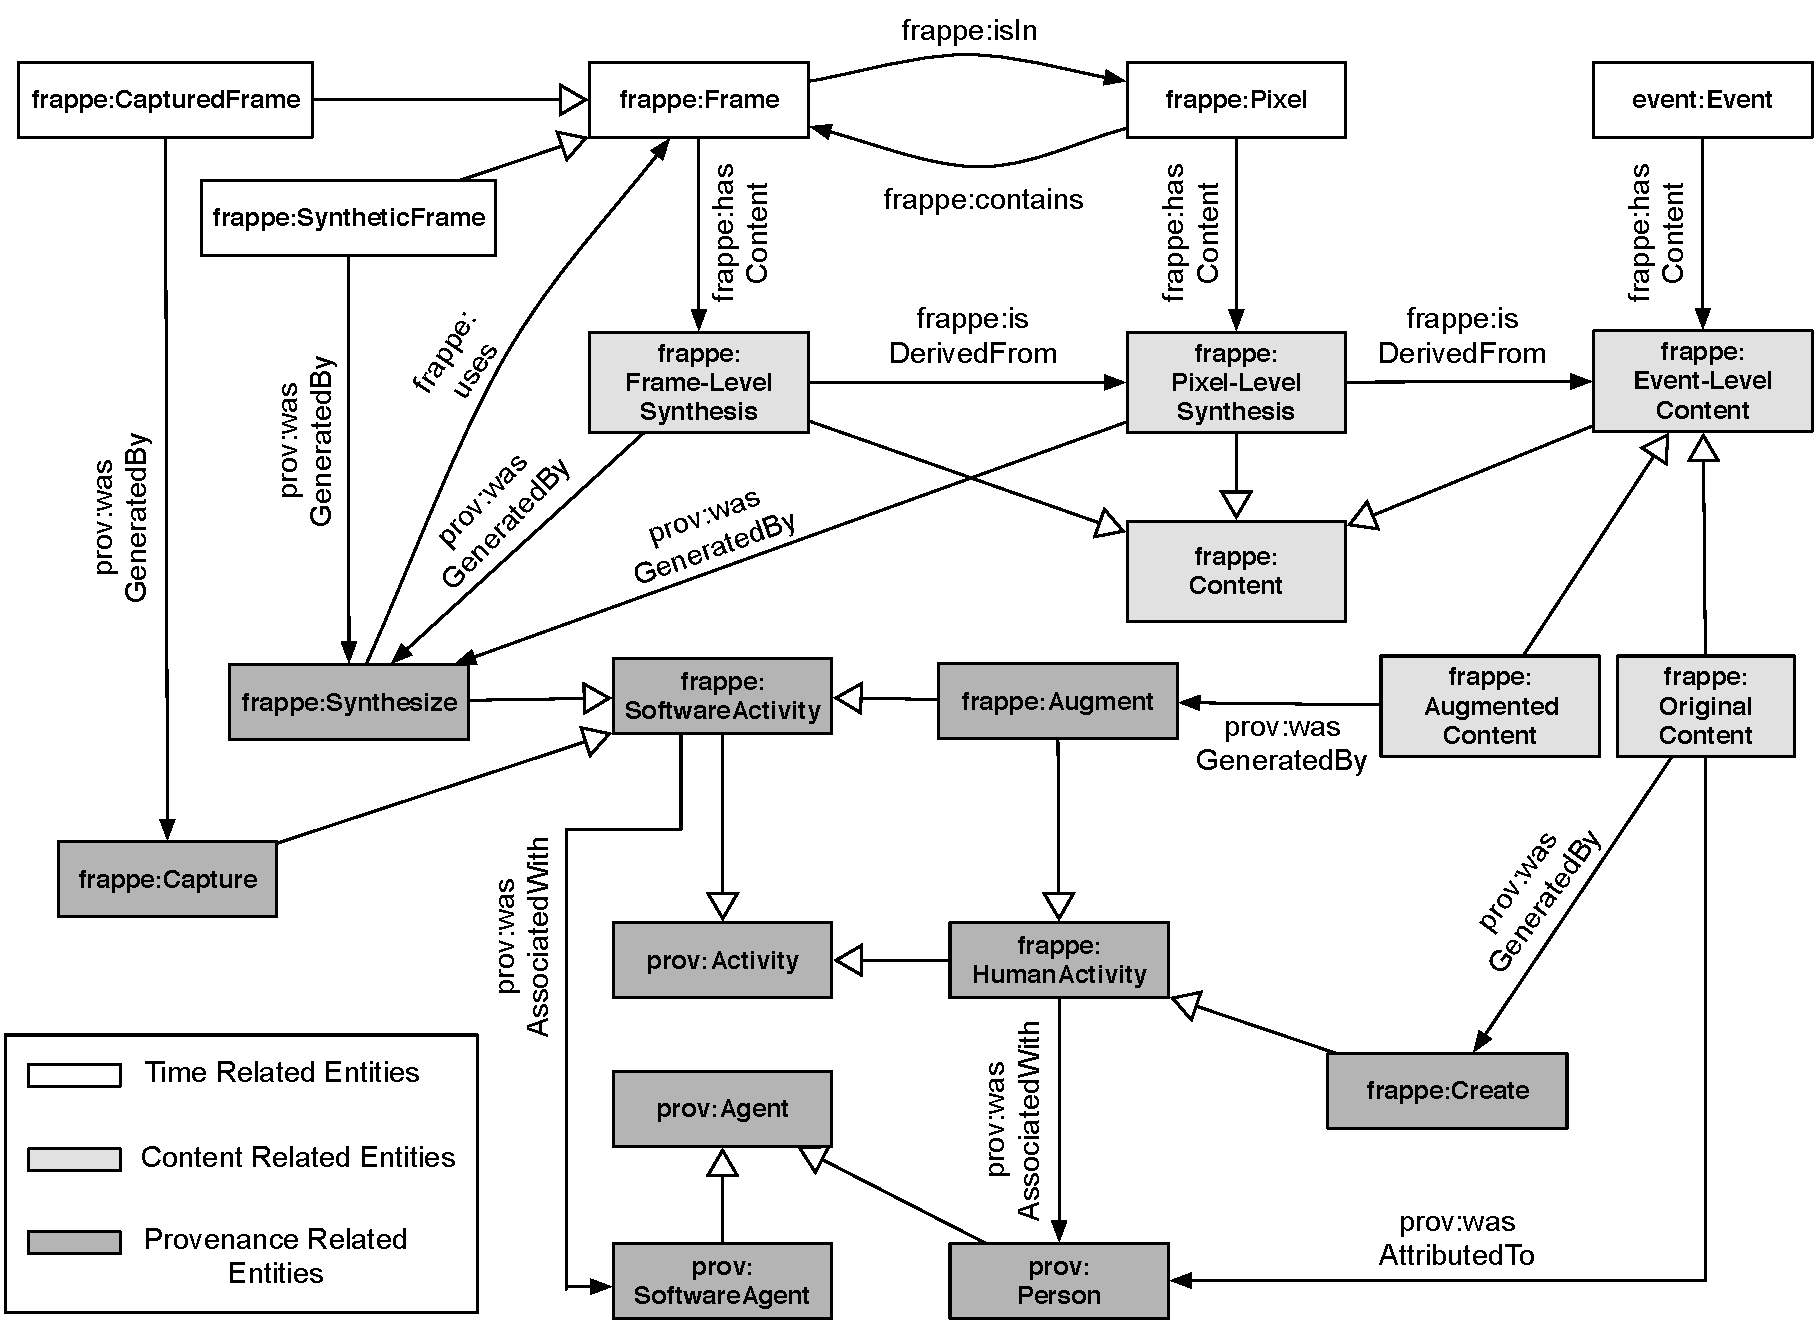
\includegraphics[width=0.95\textwidth]{img/conceptual-model-extended-core}
\caption{The extended version of the \frappe{} model, represented as a colored UML diagram highlighting time-, content-, and provenance- related concepts.}
\label{fig:extended-core}
\end{figure} 

The temporal fragment (the classes \textsf{Frame}, \textsf{Pixel} and \textsf{Event}) and the spatial fragment (the classes \textsf{Grid}, \textsf{Cell} and \textsf{Place}) are inherited from \frappe{} 1.0.
For a detailed description of these parts we refer the reader to Section~\ref{sec:conc-fr-1-mod}

In \frappe{} 2.0, the content can be associated to the time-varying classes and carries information about the event it is associated to.
At event level the content can be \textsf{Original} or \textsf{Augmented}. The original content represents a simple measure or description of a phenomenon, while any enrichment of an original content produces an augmented content.
For instance in a \textit{Tweet} related to the Museum of Modern Art (MOMA),  the \textsf{OriginalContent}, in form of a text, contains different entities presented in different surface forms (e.g., moMA, Museum of Modern Art, etc). The \textsf{Augmentation} allows to link those surface forms to a single db-pedia entity\footnote{\url{http://dbpedia.org/page/Museum_of_Modern_Art}} (see Listing~\ref{lst:sm}).
The content related to \textsf{Pixel} or \textsf{Frame} is \textsf{Synthetic} and it is derived by processing event-related contents. 

In the extended provenance fragment of \frappe{} 2.0, the \textsf{Agent} concept is explicitly defined.
Each activity is performed either by a \textsf{HumanAgent} or by a \textsf{SoftwareAgent}. Consequently, the two \textsf{Agent}s \textsf{wasAssociatedTo}, respectively, \textsf{HumanActivity} or \textsf{SoftwareActivity}. 
On the one hand, an example of \textsf{HumanActivity} is the \textsf{Create} activity, exploited to create an \textsf{OriginalContent}. On the other hand, a \textsf{SoftwareActivity} can be exemplified by the \textsf{Synthesize} activity, used to create a \textsf{Synthetic} content associated to a \textsf{Pixel} or a \textsf{Frame}.

We developed \frappe{} 2.0 keeping in mind the evaluation based on Tom Gruber's principles presented in Section~\ref{sec:conc-fr-1-eval} and it also complies to them.
\frappe{} 2.0 keeps satisfying the \textit{clarity} principles because we add common terms in provenance and content analytics domains. \frappe{} 2.0 remains as general as possible in order to satisfy the \textit{minimal encoding bias} and the \textit{minimal ontological commitment} principles. \frappe{} 2.0 is still \textit{coherent} and the use cases in the Chapter~\ref{ch:case-studies} demonstrates its \textit{extendibility}.

\section{\frappe{} 2.0 and Urban Data Analysis} \label{sec:conc-fr-2-analysis}

In this section, we summarize the methods we use in exploiting \frappe{} to enable the three classic dimensions of the urban data analysis (see Section~\ref{sec:uda-analysis}).
The use cases, presented in Chapter~\ref{ch:case-studies}, offer an overview of the \frappe{} capabilities in enabling all the classic urban data analysis categories.

Concerning the Content Analysis, as mentioned in the Section~\ref{sec:conc-fr-2}, \frappe{} enables the association of the information content to an event, with all the indirect information related to time and space.

\begin{figure}[p]
\begin{minipage}{0.95\linewidth}
\begin{lstlisting}[label={lst:sm}, caption={The \frappe{} representation of a social message}, style=N3]
@prefix frappe:<http://streamreasoning.org/ontologies/frappe#>
@prefix frPlace: <http://streamreasoning.org/frappe/Places/> .
@prefix frEvent: <http://streamreasoning.org/frappe/Events/> .
@prefix frContent: <http://streamreasoning.org/frappe/Content/> .
@prefix frAct: <http://streamreasoning.org/frappe/Activity/> .
@prefix frAgent: <http://streamreasoning.org/frappe/Agent/> .
@prefix frEntity: <http://streamreasoning.org/frappe/Entity/> .
@prefix xsd:<http://www.w3.org/2001/XMLSchema#>
@prefix time:<http://www.w3.org/2006/time#>
@prefix prov:<http://www.w3.org/ns/prov#>
@prefix event:<http://purl.org/NET/c4dm/event.owl#>
@prefix rdfs:<http://www.w3.org/2000/01/rdf-schema#>

frEvent:E a frappe:messageSending ; 
  a event:Event ;
  event:time [ a time:Instant ;
    time:inXSDDateTime "2018-07-10T10:00:00"^^xsd:dateTime ] ;
  frappe:location frPlace:P ;
  frappe:hasContent frContent:oc  ;
  frappe:hasContent frContent:ac  .

frContent:oc a frappe:OriginalContent ;
  frappe:litContent "At Museum of Modern Art to see Claude Monet, Water Lilies #moMA"^^xsd:string ;
  prov:wasGeneratedBy frAct:cActivity ;
  prov:wasAttributedTo frUser:user .

frAct:cActivity a frappe:Create ;
  a frappe:HumanActivity ;
  prov:wasAssociatedWith frAgent:user .
    
frAgent:user a frappe:HumanAgent ;
  a prov:Person .

frContent:oc a frappe:AugmentedContent ;
  frappe:dbPediaEntity frEntity:MOMA ;
  frappe:dbPediaEntity frEntity:Claude_Monet ;
  frappe:dbPediaEntity frEntity:Water_Lilies ;
  prov:wasGeneratedBy frAct:aActivity .

frEntity:MOMA a prov:entity ;
  prov:value ".../Museum_of_Modern_Art"^^xsd:anyURI ;

frEntity:Claude_Monet a prov:entity ;
  prov:value ".../Claude_Monet"^^xsd:anyURI ;

frEntity:Water_Lilies a prov:entity ;
  prov:value ".../Water_Lilies_(Monet_series)"^^xsd:anyURI ;
    
frAct:aActivity a frappe:Augment ;
  a frappe:SoftwareActivity ;
  prov:wasAssociatedWith frAgent:sa .

frAgent:sa a frappe:SoftwareAgent ;
  rdfs:label "DBpediaSpotlight"^^xsd:string;
\end{lstlisting}
\end{minipage}
\end{figure}

Listing~\ref{lst:sm} represents the sending event of a micropost by a social media user.
The listing mainly focuses on the \frappe{} 2.0 extensions (content and provenance).
According to the \frappe{} conceptual model, the \textsf{messageSending} \textsf{Event} is described by a set of properties, including the \textsf{Event-RelatedContent}.
\frappe{} 2.0 distinguishes between two different types of this content, the \textsf{OriginalContent} and the \textsf{AugmentedContent}.
In the example, the \textsf{OriginalContent} is the text of the message and is produced by a \textsf{Create} activity, performed by a \textsf{Person}. Contrariwise, the \textsf{AugmentedContent} is created by the DBpediaSpotlight \textsf{SoftwareAgent} that automatically extract the DBpedia entities from the \textsf{OriginalContent}.

\frappe{} enables the Spatial Analysis mainly through the concepts of \textsf{Grid} and \textsf{Cell}. 
Moreover, thanks to their common sense, the \textsf{Grid} and \textsf{Cell} concepts improve the understandability and navigability of geographical-based content. 
They can be instantiated in multiple ways: we may define different types of grids and cells, based on the specific data sets and on the analysis needs. We identify three main categories of grids: 

\begin{itemize}
\item \textit{Regular squared grid}:  a regular \textsf{Grid} dividing the physical space in cells that are uniform for shape, size, and positioning. For instance, in many of our experiences around the city of Milan (see Section~\ref{sec:cs-mdw}), we defined a \textsf{Grid} of 100 x 100 \textsf{Cell}s, each \textsf{Cell} having a size of 250 x 250 meters.

\item \textit{Irregular grid with official business-driven meaning}: a \textsf{Grid} of \textsf{Cell}s that are different in shape, size and orientation based on some official definition (e.g., the boroughs or zones of a city) or based on some business specification (e.g., the commercial areas of the city). An example of this can be the official city districts defined by the municipality or the areas where a large \textsf{Event} is located. During our experiences in Milan we used the definitions of the official MDW areas to perform aggregated analysis on the data (see Section~\ref{sec:cs-mdw}).

\item \textit{Irregular grid with data-driven definition}: a \textsf{Grid} of \textsf{Cell}s defined bottom-up based on the domain data available or on partial analysis and aggregations already performed on them. Some examples include the areas served by different electricity sub-stations, the mobile phone cell coverage, or the areas where mobile phone presence can be clustered with sufficient precision with respect to the location of the antennas. During our work in Como (see Section~\ref{sec:cs-como}), we experienced data-driven definition of different areas related to the mobile network coverage. 

\end{itemize}
Another important feature of the \textsf{Grid} is the coverage of the area of interests. We can define \textsf{Grid}s with \textbf{total coverage} or \textbf{partial coverage}. Typically, regular \textsf{Grid}s tend to feature total coverage, while irregular ones, especially when defined starting from business requirements, may offer only a partial coverage of the area.

All the relevant spatial analysis exposed in Section~\ref{sec:uda-analysis} (i.e., Dispersion, Distance and relation to places, Correlation and Prediction) can be performed exploiting the concept of \textsf{Grid} and \textsf{Cell}.

The Temporal analysis in \frappe{} can be described as the study of the evolution and spreading of signals captured by \textsf{Pixel}s, which refers to \textsf{Cell}s, over time in different \textsf{Frame}s.
\frappe{} enables all the categories of the temporal analysis described in Section~\ref{sec:uda-analysis}.
The \textsf{Description} in \frappe{} describe the signal \textsf{captured} by \textsf{Pixel}-level contents to create a time-series. \frappe{} enables the \textsf{Correlation}, \textsf{Prediction}, \textsf{Anomaly detection} and \textsf{Causality} analysis exploiting the concepts of \textsf{Pixel} and \textsf{Frame}. 

Finally, \frappe{} exploits the links between \textsf{Cell} and \textsf{Pixel}, \textsf{Grid} and \textsf{Frame} to enable the combination of time and space analysis. 

\section{Conclusion}
In this chapter, we study the problem of modeling spatio-temporal data to enable analyses that involve time, space and content aspects of the data. 
The growing availability of geo-located time-varying data, in particular in the urban environment, increased the needs for an holistic conceptual model to describe the data itself, its dynamics and to enable advanced analysis.

To address this problem, we proposed \frappe{} conceptual model. 
\frappe{} exploits digital image processing terms to tame three main dimensions of analysis: space, time, and content.
It uses image processing common terms to create a bridge between the data engineers and visual interface designers and enables visual analytics on geo-spatial time varying data.

We first developed \frappe{} 1.0 using state of the art methodology (METHONTOLOGY).
It is formalized using OWL2 and reuses already existing ontologies (see Section~\ref{sec:conc-fr-1-mod} for further details).
We then extended \frappe{} to version 2.0 by adding concepts related to the provenance and the content (see Section~\ref{sec:conc-fr-2} for additional details on the extension).

In order to validate Hypothesis \textsf{Hp.1.1}, we checked the adherence of \frappe{} 1.0 to the five Tom Gruber's principles (see Section~\ref{sec:conc-fr-1-eval}).
The \textit{clarity}, \textit{minimal encoding bias} and \textit{coherence} is respected by construction. 
Infact, the \frappe{} 1.0 definitions are documented in natural language, they are formalized using OWL2 standard and all the inferred data is meaningful and consistent.  
Moreover, \frappe{} 1.0 requires a \textit{minimal ontological commitment} because it easily allows specialization, while its \textit{extendibility} is ensured by the number of use cases that are based on it.

Our extended usage of \frappe{} 1.0 in real world use cases (see Chapter~\ref{ch:case-studies}) pushed us to create \frappe{} 2.0 that contains the formalization of the concepts that we used more often in our use cases.
They are related to the provenance of the information and to the content of the events.
Also \frappe{} 2.0 results \textit{clear}, \textit{coherent}, \textit{extendable} and with \textit{minimal encoding bias}.
Moreover, it still requires a \textit{minimal ontological commitment}, since the new concepts has been formalized because they are shared by two or more use cases.

The overall evaluation, based on Tom Gruber's Principles, validates the Hypothesis \textsf{Hp.1.1}.
The presentation of the validation of the Hypothesis \textsf{Hp.1.2} is postponed to Chapter~\ref{ch:case-studies} because it is based on the empirical evaluation of the guessability of the use cases' visualizations. 
%Computational Model
\chapter{Computational Model}\label{ch:computational}
In this chapter, we propose \river{}\footnote{The name \river, and its graphics, is inspired by the data continuously flowing one way into the system.} -- a variety-proof computational model to deal with streaming data.
Section~\ref{sec:comp-mod-intro} introduces the problem of dealing with data characterized by high \textit{Variety} and \textit{Velocity}without forgetting \textit{Volume}.
In Section~\ref{sec:comp-mod-sol}, we propose a) the background concepts that underpin \river{}, b) the semantics and textual syntax of the operators of \river{} and c) the Pipeline Definition Language -- a graphic language to ease the modeling of \river{} plans.


the computational model operators together with their semantics and textual syntaxes and the Pipeline Definition Language, -- a graphic language to ease the development of computational plans.

\section{Introduction and Problem Statement} \label{sec:comp-mod-intro}
In our case studies (see Chapter~\ref{ch:case-studies}), we noticed that data can come from different sources that vary in format (\textit{Variety}) and size (\textit{Volume}), but it  always flows (\textit{Velocity}). Even what we normally call "\textit{static data}", e.g.,  a city street network, is not immutable over time, it  slowly evolves.

In 2013, we presented SLD (see Section~\ref{sec:rsp-mid}), a middleware to ease the deployment of an RSP engine in a real world scenario characterized by heterogeneous streaming data.
In five years of SLD usage, we learned that using RDF streams is valuable when (i) data are naturally represented as graphs, (e.g., micro-posts in the larger social graph) and when (ii) the availability of popular vocabularies eases the development of adapters that semantically annotate the external data flows.
For instance, we wrote adapters that annotate streams from the major social networks using SIOC~\cite{DBLP:journals/ijwbc/BreslinDHB06}.

However, we also found out several weaknesses of the RDF-only approach: (i) RDF streams cannot be found in the wild, yet, JSON is largely used in practice (e.g., Twitter Streaming APIs\footnote{\url{https://dev.twitter.com/streaming/overview}} and W3C activity stream 2.0 working draft\footnote{\url{http://www.w3.org/TR/activitystreams-core/}}) and (ii) the results of a continuous computation are often relational and forcing them into an RDF stream is suboptimal.
%(e.g., a user would naturally use the REGISTER QUERY ... AS SELECT ... form instead of REGISTER STREAM ... AS CONSTRUCT ... one. It takes three triples to state how many times a hashtag appears in the micro-posts observed in 1 minute, while the tuple $\langle$timestamp, hashtag, count$\rangle$ is more succinct).

Those reflections inspired the idea to work with the data in its original format as long as possible to reduce the latency caused by the data transformations at ingestion time. We named this approach \textit{Lazy Transformation}.

In order to investigate how \textit{Lazy Transformation} helps in address our research questions -- \textit{Is it possible to continuously ingest and reactively analyses a variety of streaming urban data in order to visualize emerging patterns and their dynamics?} -- we formulate the hypothesis:

\begin{itemize}[leftmargin=42pt]
\item[\textsf{Hp.2.1}] The implementation of a streaming computational model that defers as long as possible the data transformation demands less resources and better approximates the correct answer under stress conditions than an implementation of a computational model that cast data into RDF at ingestion time.
\end{itemize}

\section{\texorpdfstring{\protect\river{}}{RIVER}}\label{sec:comp-mod-sol}
In the next sections, we present \river{}, a variety proof streaming computational model built around the idea of \textit{Lazy Transformation}.

In Section~\ref{sec:comp-mod-sol-pre}, we introduce the background concepts that underpin \river{}.
Section~\ref{sec:comp-mod-sol-lang} presents in detail the semantics and the textual syntaxes of the \river{}'s operators, the Pipeline Definition Language (PDL) -- a graphic syntax to abstract the implementation complexity -- and, eventually, examples of physical languages (e.g., EPL, SQL, SPARQL, etc.) to implement the \river{}'s operators. All of those concepts are presented through a running example.
Finally, in Section~\ref{sec:comp-mod-sol-arch}, we present a reference architecture for systems that implement \river{}.

\subsection{Preliminaries}\label{sec:comp-mod-sol-pre}
Based on the considerations resulting from the development of our conceptual model (see Chapter~\ref{ch:conceptual}) and on our past experiences (see Chapter~\ref{ch:case-studies}), we identify two principles that inspire \river{}.

\textbf{(P1)} \textit{everything is a data stream}. According to this principle, a variety-proof stream processing engine must indifferently ingest data with different velocities from any sources and of any size. 

For instance, the movements of a car is a \textit{fast} data stream where the information flow records the identity, the positions and the speeds of the cars. In this case, the distance between two subsequent observations can be seconds. On the other side, a city road is a \textit{slowly evolving} data stream, where the information flow records, for instance, the addition of a bike lane.
In this second case, the distance between two subsequent observations can be days or months. 

The continuous nature of data streams, and the importance of the information extracted by the most fresh data, require such a category of engine to avoid data loss and, consequently, to implement our second principle: \textbf{(P2)} \textit{Continuous Ingestion}. The data in input is continuously captured by the system and, once arrived, it is marked with an increasing timestamp. Notably, some data sources may natively include their own timestamp too (namely, the application timestamp, presented in Section~\ref{sec:secret}). It is worth to note that a continuous ingestion mechanism helps to avoid data losses, but continuous analysis is not always needed; an analysis can be reactive even if postponed (see Section~\ref{sec:comp-mod-eval-cost}).

In order to challenge the hypothesis \textsf{Hp.2.1}, we propose the \textit{lazy transformation} approach. 
A variety-proof stream processing engine operates on the data in its original format as long as it can, and it transforms data only if it really needs to do so. Indeed, operations like projections, filters or aggregations can operate on generic data without requiring to cast all data in a single format (such as RDF). Therefore, for those operations, we can delay transformations. Contrariwise, a join operation on data of different data format (e.g., a CVS table and a JSON tree), normally, first requires to cast data in a common format (e.g., the relational one) and then perform the join. 

So, this kind of system must rely on data of generic type $\mathrm{T}$.

\begin{Definition}
(Type to-be-specified-later) A type to-be-specified-later $\mathrm{T}$ represents the generic type of the atomic object flowing into the system.
\end{Definition}

Together with the definition of time (already reported in Section~\ref{sec:stream-proc}), we can define the information flowing into this kind of systems as a Generic Data Stream.

\begin{Definition}
(Time) The time $\mathcal{T}$ is an infinite, discrete, ordered sequence of time instants $(\tau_1,\tau_2,..., \tau_n)$, where $\tau_i \in \mathbb{N}$. A time unit is the difference between two consecutive time instants $(\tau_{i+1} - \tau_i)$ and it is constant.
\end{Definition}

\begin{Definition}
(Generic Data Stream) A Generic Data Stream S$\langle\mathrm{T}\rangle$ is a potentially unbounded sequence of timestamped data items $(d_i,\tau_i)$:
\noindent\begin{align*}
S = (d_1,\tau_1), (d_2,\tau_2), \ldots, (d_n,\tau_n)
\end{align*}  
where $d_i$ is of type $\mathrm{T}$, $\tau_i \in \mathcal{T}$ is the associated time instant and $\tau_i<\tau_{i+1}$.
\end{Definition}

Note that the time instants associated to data items is monotonically increasing. We do not allow contemporary ingestion, because we consider the time as a form of punctuation. 
So, the data items $d_i$ in a Generic Data Stream S$\langle\mathrm{T}\rangle$ is of \textit{types to-be-specified-later} $\mathrm{T}$, and, for instance, it can be, indifferently, a tree representation of a JSON document, a set of tuples in CSV or in parquet format, or a graph in RDF.

\textit{Generic Functions} and \textit{Generic Types}~\cite{DBLP:conf/dagstuhl/1998gp} represents the natural abstraction to model the operations that manipulate information in accordance with the \textit{lazy transformation} approach. 

Let us now define a Generic Time-Varying Collection as:

\begin{Definition}
(Generic Time-Varying Collection) A Generic Time-Varying Collection C$\langle\mathrm{T}\rangle$ is a mapping from $\mathcal{T}$ to a finite but unbounded bag of data items $d_i$, where $d_i$ is of type $\mathrm{T}$. 
\end{Definition}

Differently from a Generic Time-Varying Collection, a Generic Instantaneous Collection defines an unordered bag of data items at a specific time instant.

\begin{Definition}
(Generic Instantaneous Collection) A Generic Instantaneous Collection  C$\langle\mathrm{T}\rangle(\tau)$ is the bag of data items in a collection at $\tau$, a given point in time . 
\end{Definition}

\subsection{\texorpdfstring{\protect\river{}}{RIVER}'s Operators and the Pipeline Definition Language}\label{sec:comp-mod-sol-lang}

\river{} computational model enables users to define computational plans, in the form of pipelines (formally DAGs\footnote{A finite directed graph with no directed cycles.}), composed by different operators that take care of ingesting, processing and emitting Generic Data Streams.
In order to ease the definition of the computational plans, we propose the Pipeline Definition Language (PDL).
It defines the graphical syntax of the operators.

\begin{figure}[t]
  \centering
  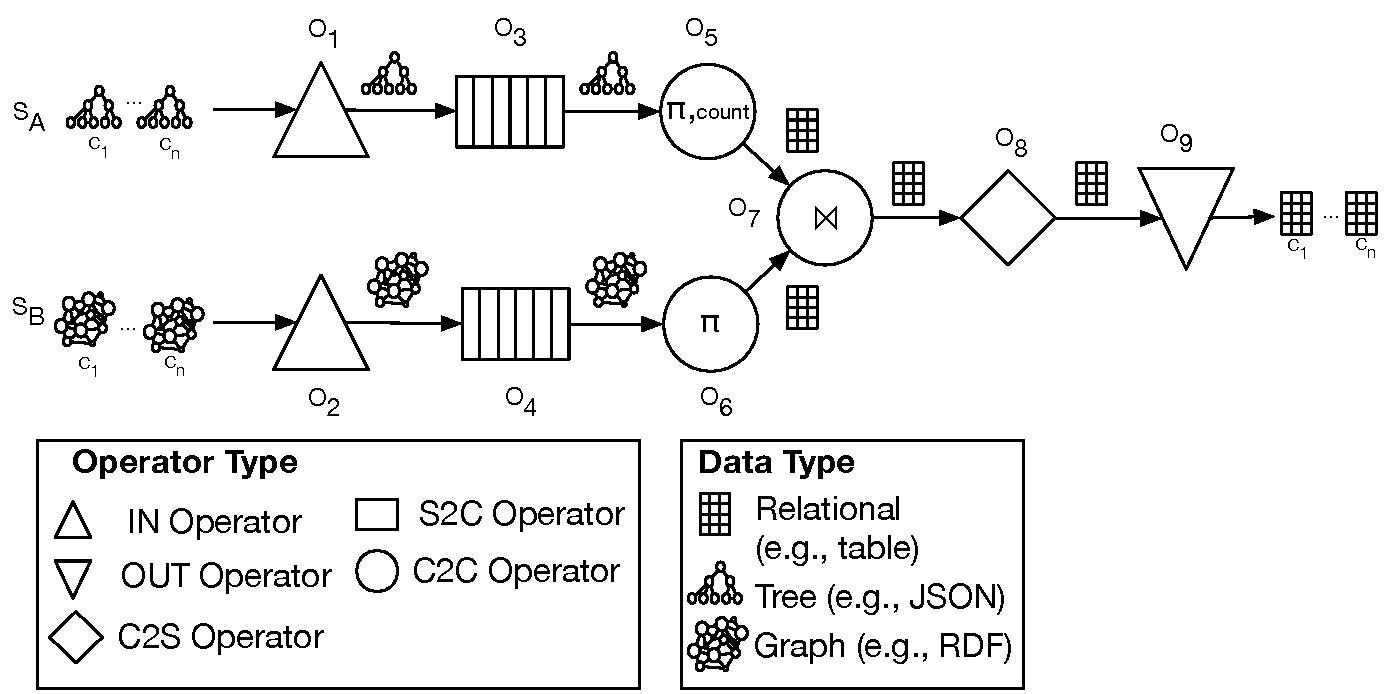
\includegraphics[width=0.92\textwidth]{img/computational-model-syntax-example-ODL}
  \caption{Pipeline that presents an example of the operators and of the typical data type produced during the computation.}
  \label{fig:sti_ex}
\end{figure} 

The reader will be guided into the details via the running example depicted in Figure~\ref{fig:sti_ex}.
The presented operators and symbols will be detailed discussed in the next paragraphs.

\begin{Example}
The example, depicted in Figure~\ref{fig:sti_ex}, represents the pipeline to deal with a typical social media analytics use case.
The inputs to the pipeline are the post stream S$_A$ and the users' friend network, the stream S$_B$, in the form of graph. The two streams have to be joined in order to connect users with common friends in the same location.
\end{Example}
 
More formally, Figure~\ref{fig:cm-op} depicts the five classes of \river{} operators and their interactions. 
The operators, defined as S2C$\langle\mathrm{T}\rangle$, C2C$\langle\mathrm{T},\mathrm{T^{\prime}}\rangle$ and C2S$\langle\mathrm{T}\rangle$ in \river{}, are inspired to the CQL processing model (see Section~\ref{sec:CQL}), and allow to move from S$\langle\mathrm{T}\rangle$ to C$\langle\mathrm{T}\rangle$ and vice-versa.
In addition to the CQL-like operators, we introduce the \textit{ingestion} (defined as IN$\langle\mathrm{T}\rangle$ in \river{}) and \textit{emission} (defined as OUT$\langle\mathrm{T}\rangle$ in \river{}) operators.
They, respectively, ingest and emit streams of data to/from a system implemented using \river{} computational model.

In the next paragraphs, we report the details of the operators and present, for each of them, its formal definition, its graphical syntax in PDL, the examples of physical languages for its implementation and its role in the running example (see Figure~\ref{fig:sti_ex}).

\begin{figure}[t]
    \centering
    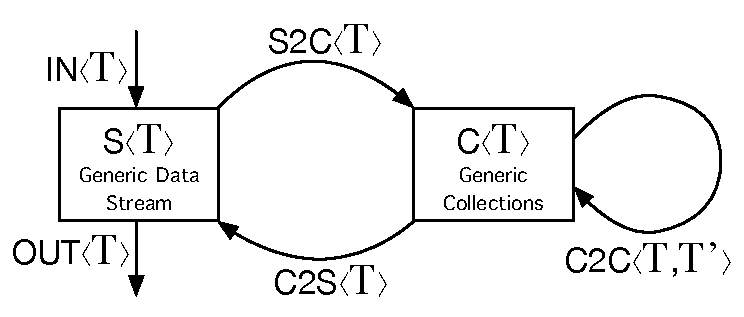
\includegraphics[width=0.8\textwidth]{img/computational-model-operators}
    \caption{Overview of \textnormal{\protect\river{}} operators.}
    \label{fig:cm-op}
\end{figure}

\medskip
\noindent
\textbf{Ingestion Operator}
\medskip

\begin{Definition}
(Ingestion operator) A IN$\langle\mathrm{T}\rangle$ operator takes an external data flow and inject the items into the system creating a new S$\langle\mathrm{T}\rangle$. 
The ingestion operator is type-agnostic, it works independently from the external source data-type.
It always transform the items in the external data flow into internal generics (defined as $\langle\mathrm{T}\rangle$).
\end{Definition}

\noindent
In PDL we introduce the symbol $\bigtriangleup$ to represent the Ingestion operator.

\begin{Example}
(cont'd) The external data flows S$_A$ and S$_B$ need to be ingested in order to be analyzed.
O$_1$ and O$_2$ are implementations of IN$\langle\mathrm{T}\rangle$ operator for Twitter. 
They contain the logic for connecting to twitter and retrieve the requested informations.
On the one hand, O$_1$ takes care of the external data flow S$_A$, by connecting to the Twitter streaming API and ingesting JSON Trees as generics $\langle\mathrm{T}\rangle$.
Listing~\ref{lst:o1_res} shows the resulting JSON.

\begin{figure}[ht]
\begin{minipage}{0.95\linewidth}
\begin{lstlisting}[caption={Example of the data resulting by the ingestion operation performed by O$_1$.},label=lst:o1_res,style=JSON]
  {
    "data": [{
      "user_id": ":Alice",
      "content": "breathless at #moma",
      "hashtag": [
         { 
           "tag_id":"t1"
           "text":"moma"
         }
      ],
      "latitude":40.761620,
      "longitude":-73.977257,
      "time":"2018-09-30T09:00:00"
     }
    ]
   }
\end{lstlisting}
\end{minipage}
\end{figure}

On the other hand, O$_1$ manages the external data flow S$_B$, by polling the Twitter REST API and ingesting RDF Graph as generics $\langle\mathrm{T}\rangle$.
Listing~\ref{lst:o2_res} shows the resulting RDF Graph.

\begin{figure}[ht]
\begin{minipage}{0.95\linewidth}
\begin{lstlisting}[caption={Example of the data resulting by the ingestion operation performed by O$_2$.},label=lst:o2_res,style=N3]
:Alice a :User ;
    :userName "Alice"^^xsd:string ;
    :birthDate "1980-06-21"^^xsd:date ;
    :hasFriend :Bob .
\end{lstlisting}
\end{minipage}
\end{figure}

\end{Example}

\medskip
\noindent
\textbf{Stream-to-collection Operator}
\medskip

\begin{Definition}
(Stream-to-collection operator) A S2C$\langle\mathrm{T}\rangle$ operator transforms a portion of a potentially infinite Generic Data Stream S$\langle\mathrm{T}\rangle$ into a Generic Time-Varying Collection C$\langle\mathrm{T}\rangle$.
S2C$\langle\mathrm{T}\rangle$ operator type-agnostic, the operation is completely independent from $\mathrm{T}$.
\end{Definition}

Similarly to CQL, the implementations of the S2C$\langle\mathrm{T}\rangle$ operator are based on the concept of \textit{sliding window}.
In particular, we can define the concept of Generic Data Window.

\begin{Definition}
(Generic Data Window) A window W$\langle\mathrm{T}\rangle(S)$ is a set of data items (d$_1$, ..., d$_n$), of type $\mathrm{T}$, extracted from a Generic Data Stream S$\langle\mathrm{T}\rangle$. 
\end{Definition}

Exploiting this concept we can now define two classes of Generic Data Window.
The \textit{time-based} Sliding Generic Data Window and the \textit{tuple-based} Generic Data Window.

Time-based Sliding Generic Data Window operator defines its output by sliding an interval of $\mathrm{K}$ time units over the stream S$\langle\mathrm{T}\rangle$.

\begin{Definition}
(Time-based Sliding Generic Data Window) A Time-based Sliding Generic Data Window on a stream S$\langle\mathrm{T}\rangle$ takes a time-interval $\mathrm{K}$ as a parameter and is specified by following S$\langle\mathrm{T}\rangle$ in the query with [Range $\mathrm{K}$].
The output Generic Instantaneous Collection C$\langle\mathrm{T}\rangle(\tau)$ of S$\langle\mathrm{T}\rangle$[Range $\mathrm{K}$] is defined as:
\noindent\begin{align*}
C\langle\mathrm{T}\rangle(\tau)=\{s \mid \langle s,\tau' \rangle \in S\langle\mathrm{T}\rangle \wedge (\tau' \leq \tau) \wedge (\tau' \geq \max\{\tau - \mathrm{K},0\})\}
\end{align*}  
\end{Definition}

Tuple-based Sliding Generic Data Window operator defines its output by sliding a window of size $\mathrm{N}$ data items over the stream S$\langle\mathrm{T}\rangle$.
\begin{Definition}
(Tuple-based Sliding Generic Data Window) A Tuple-based Sliding Generic Data Window takes a positive integer $\mathrm{N}$ as a parameter and is specified by following S$\langle\mathrm{T}\rangle$ in the query with [Rows $\mathrm{N}$].
The Generic Instantaneous Collection C$\langle\mathrm{T}\rangle(\tau)$ of S$\langle\mathrm{T}\rangle$[Rows $\mathrm{N}$], consists of data items of type $\mathrm{T}$ obtained from the $\mathrm{N}$ elements with the largest timestamps in S$\langle\mathrm{T}\rangle$ no greater than $\tau$.
\end{Definition}

%Partitioned Sliding Generic Data Window logically partitions S$\langle\mathrm{T}\rangle$ into sub-streams based on equality of attributes $A_1, ..., A_k$, computes a Tuple-based Sliding Generic Data Window of size $N$ on each sub-stream, then produce a Generic Collection which contains the union of these sub-windows.

%\begin{Definition}
%(Partitioned Sliding Generic Data Window) A Partitioned Sliding Generic Data Window on a stream S$\langle\mathrm{T}\rangle$ takes a positive integer N and a subset $\{A_1, ..., A_k\}$ of S attributes as parameters. It is specified by following S$\langle\mathrm{T}\rangle$ in the query with [Partition By $A_1, ..., A_k$ Rows N].
%Formally, a data item d of type $\mathrm{T}$ with values $a_1, ..., a_k$ for attributes $A_1, ..., A_k$ occurs in output Generic Instantaneous Collection C$\langle\mathrm{T}\rangle(\tau)$ iff exists an element $\langle d,\tau' \rangle \in S\langle\mathrm{T}\rangle$ such that $\tau' \leq \tau$ is among the N largest timestamps among elements whose tuples have values $a_1, ..., a_k$ for attributes $A_1, ..., A_k$
%\end{Definition}

\noindent
In PDL, we use the symbol $\hrectangle$ to represent the S2C$\langle\mathrm{T}\rangle$ operator. 
In particular, the symbol related to the S2C$\langle\mathrm{T}\rangle$ operators can give an hint about the operator's implementation.
For instance, the S2C$\langle\mathrm{T}\rangle$ operators O$_3$ and O$_4$, proposed in Figure~\ref{fig:sti_ex}, are implemented as two windowers.

\begin{Example}
(cont'd) The operators O$_3$ and O$_4$ apply Time-based sliding window operations to the streams resulting from the operators O$_1$ and O$_2$.
Operator O$_3$ is a S2C$\langle Tree \rangle$, while O$_4$ implements a S2C$\langle Graph \rangle$

As anticipated in the introduction, we report the physical implementation of some operators. 
In this case, both O$_3$ and O$_4$ can be implemented exploiting ESPER engine (See Section~\ref{sec:esper-epl}) and using the EPL clause TIME to create sliding windows with 1 minute duration.
Note that the operators are completely agnostic to the data type. O$_3$ and O$_4$ are the same query, except for the name of the stream (See Linting~\ref{lst:epl-win-03} and Linting~\ref{lst:epl-win-04}).

\begin{figure}[ht]
\begin{minipage}{0.95\linewidth}
\begin{lstlisting}[caption={EPL query, applied by O$_3$ operator, to window the stream of JSON trees},label=lst:epl-win-03,style=ESPER]
     SELECT * FROM treeEvent#TIME(1 MIN) 
\end{lstlisting}
\end{minipage}
\end{figure}

\begin{figure}[ht]
\begin{minipage}{0.95\linewidth}
\begin{lstlisting}[caption={EPL query, applied by O$_4$ operator, to window the stream of RDF graphs},label=lst:epl-win-04,style=ESPER]
     SELECT * FROM graphEvent#TIME(1 MIN) 
\end{lstlisting}
\end{minipage}
\end{figure}

The proposed EPL queries, produce two Generic Instantaneous Collections that contain, respectively, the JSON trees and the RDF graphs ingested in the last minute, without apply any transformation to the data items.

\begin{figure}[p]
\begin{minipage}{0.95\linewidth}
\begin{lstlisting}[caption={Example of result of the O$_3$ operators.},label=lst:o3_res,style=JSON]
  {
    "data": [{
      "user_id": ":Alice",
      "content": "breathless at #moma",
      "hashtag": [
         { 
           "tag_id":"t1"
           "text":"moma"
         }
      ],
      "latitude":40.761620,
      "longitude":-73.977257,
      "time":"2018-09-30T09:00:00"
     },{
      "user_id": ":David",
      "content": "Morning at #moma",
      "hashtag": [
         { 
           "tag_id":"t1"
           "text":"moma"
         }
      ],
      "latitude":40.761620,
      "longitude":-73.977257,
      "time":"2018-09-30T09:00:30"
     },{
      "user_id": ":Carl",
      "content": "Spending my day at #MoMA",
      "hashtag": [
         { 
           "tag_id":"t2"
           "text":"MoMA"
         }
      ],
      "latitude":40.761620,
      "longitude":-73.977257,
      "time":"2018-09-30T09:00:45"
     },{
      "user_id": ":Alice",
      "content": "#picasso at #moma",
      "hashtag": [
         { 
           "tag_id":"t1"
           "text":"moma"
         }, { 
           "tag_id":"t3"
           "text":"picasso"
         }
      ],
      "latitude":40.761620,
      "longitude":-73.977257,
      "time":"2018-09-30T09:00:55"
     }
    ]
  }
\end{lstlisting}
\end{minipage}
\end{figure}

Before producing the output, in order to enable query operation for the downstream operators, O$_3$ merges the different JSON trees in a single JSON tree which contains an array of elements (see Listing~\ref{lst:o3_res}).
The operator O$_4$ works in a similar way on the input stream of RDF graphs. It windows the stream and creates a single RDF graph in output that contains all the information that entered the system in the last minute (see Listing~\ref{lst:o4_res}).

\begin{figure}[ht]
\begin{minipage}{0.95\linewidth}
\begin{lstlisting}[caption={Example of result of the O$_4$ operator.},label=lst:o4_res,style=N3]
:Alice a :User ;
    :userName "Alice"^^xsd:string ;
    :birthDate "1980-06-21"^^xsd:date ;
    :hasFriend :Bob .
:Bob a :User ;
    :userName "Bob"^^xsd:string ;
    :birthDate "1965-08-10"^^xsd:date ;
    :hasFriend :Alice ;
    :hasFriend :Carl .
:Carl a :User ;
    :userName "Carl"^^xsd:string ;
    :birthDate "1965-05-15"^^xsd:date ;
    :hasFriend :Bob .
\end{lstlisting}
\end{minipage}
\end{figure}

\end{Example}

\medskip
\noindent
\textbf{Collection-to-collection Operator}
\medskip

\begin{Definition}
(Collection-to-collection operator) A C2C$\langle\mathrm{T},\mathrm{T^{\prime}}\rangle)$ operator transforms one or more Generic Instantaneous Collection C$\langle\mathrm{T}\rangle(\tau)$ in input into a single Generic Instantaneous Collection C$\langle\mathrm{T'}\rangle(\tau)$.
\end{Definition}

The implementations of this class of operators are tailored on the different data format, e.g., JSONiq operators process  JSON,  SQL operators process relational table, SPARQL operators process RDF graph, etc. Notably, $\mathrm{T}$ and $\mathrm{T^{\prime}}$ can be of different types, but they can also be of the same type. For instance, a filter on a table, on a tree or on a graph extract tuples, sub-trees or sub-graphs maintaining the original data type. Contrariwise, as we noticed above, a count aggregation transform the original data type into a table.

\noindent
In PDL, we use the symbol $\bigcirc$ to represent the C2C$\langle\mathrm{T},\mathrm{T^{\prime}}\rangle$ operator.

\begin{Example}
(cont'd) The operator O$_5$ is a C2C$\langle Tree,Relational\rangle$ and performs an aggregation on the output of the O$_3$ operator. 
The JSON object from O$_3$ contains the list of the posts that have entered the system in the last minute.
Differently from the generic EPL queries (see Listing~\ref{lst:epl-win-03} and Listing~\ref{lst:epl-win-04}), in order to perform the aggregation query (presented in the Listing~\ref{lst:oc_query}) the operator O$_5$ needs to know the data format in advance. As specified in the operator's definition, the implementation of the operator change with the input data type and can be choose at design time.

\begin{figure}[ht]
\begin{minipage}{0.95\linewidth}
\begin{lstlisting}[caption={JSONiq Query for aggregating JSON element, applied by the operators O$_5$.},label=lst:oc_query,style=JSONIQ]
FOR $user IN COLLECTION("data")
GROUP BY $user_id := $user.user_id
RETURN { "user_id" : $user_id, "count" : COUNT($user) }
\end{lstlisting}
\end{minipage}
\end{figure}

The query in Listing~\ref{lst:oc_query} counts the elements in the list, grouped by user\_id, and produces a relational table. 

\begin{table}[ht]
\centering
\caption{Example of result produced by the O$_5$ operator.}
\label{tbl:oc_res}
    \begin{tabular}{|c|c|}
        \hline
        \textbf{user\_id} & \textbf{count} \\ \hline
        :Alice             & 2              \\ \hline
        :Carl              & 1              \\ \hline
        :David             & 1              \\ \hline
    \end{tabular}
\end{table}

Table~\ref{tbl:oc_res} presents the output of O$_5$: a relational table with the user\_id and the associated count.

In the other branch of the pipeline, which manage the slowly evolving data that enter the system in RDF graph format, the operator O$_6$, similarly to the operator O$_5$, extracts information related only to the users who have at least one friend in common.  

\begin{figure}[ht]
\begin{minipage}{0.95\linewidth}
\begin{lstlisting}[caption={SPAQL query applied by operator O$_6$ to the RDF stream to project information about the user.},label=lst:od_query,style=SPARQL]
SELECT ?user_id ?name ?birthDate
WHERE {
    ?user1 a :User;
    :user_id ?user_id ;
    :userName ?name ;
    :birthDate ?birthDate ;
    :hasFriend ?commonFriends .
    ?user2 a :User;
    :hasFriend ?commonFriends .    
FILTER (?user1 != ?user2)
} 
\end{lstlisting}
\end{minipage}
\end{figure}

\medskip

Operator O$_6$ is a C2C$\langle Graph,Relational\rangle$.
It extracts information from the slowly evolving RDF graph stream via the SPARQL query presented in Listing~\ref{lst:od_query} and creates a relational table as presented in the Table~\ref{tbl:od_res}.

\begin{table}[ht]
\centering
\caption{Example of result produced by the O$_6$ operator.}
\label{tbl:od_res}
    \begin{tabular}{|c|c|c|}
        \hline
        \textbf{user\_id} & \textbf{name} & \textbf{birthDate} \\ \hline
        :Alice             & Alice         & 1980-06-21         \\ \hline
        :Carl              & Carl          & 1965-05-15         \\ \hline
    \end{tabular}
\end{table}

The operator O$_7$ joins two collections C$\langle Relational\rangle$ from the two branches using the user\_id as key and produces an enriched Collection C$\langle Relational\rangle$. 
Table~\ref{tbl:oe_res} presents the results of the join operation. 
It contains the personal information of the users with at least one Friend in common, together with the count of posts tweeted in the last minute.

\begin{table}[ht]
\centering
\caption{Example of Results produced by the O$_7$ operator}
\label{tbl:oe_res}
    \begin{tabular}{|c|c|c|c|}
        \hline
        \textbf{user\_id} & \textbf{name} & \textbf{birthDate} & \textbf{count} \\ \hline
        :Alice             & Alice        & 1980-06-21         & 2              \\ \hline
        :Carl              & Carl         & 1965-05-15         & 1              \\ \hline
    \end{tabular}
\end{table}
\end{Example}

\medskip
\noindent
\textbf{Collection-to-stream Operator}
\medskip

\begin{Definition}
(Collection-to-stream operator) The C2S$\langle\mathrm{T}\rangle$ operator needs a Generic Collection C$\langle\mathrm{T}\rangle$ as input, to create a new Generic Data Stream S$\langle\mathrm{T}\rangle$ as output. 
This operator is used to emit, as a new Generic Data Stream S$\langle\mathrm{T}\rangle$, the results over time of C2C$\langle\mathrm{T},\mathrm{T^{\prime}}\rangle$ operators. 
\end{Definition}

Similarly to CQL, \river{} introduces three classes of C2S$\langle\mathrm{T}\rangle$ operators.

\begin{Definition}
(Insert Generic Data Stream) The Istream applied to Generic Collection C$\langle\mathrm{T}\rangle$ contains an element $\langle d,\tau \rangle$, with d of type $\mathrm{T}$, iff the data item d is in C$\langle\mathrm{T}\rangle(\tau)$ - C$\langle\mathrm{T}\rangle(\tau - 1)$: 
\noindent\begin{align*}
Istream(C\langle\mathrm{T}\rangle) = \bigcup_{\tau \geq 0} ((C\langle\mathrm{T}\rangle(\tau) - C\langle\mathrm{T}\rangle(\tau - 1)) \times \{\tau\}).
\end{align*} 
\end{Definition}

\begin{Definition}
(Delete Generic Data Stream) The Dstream applied to Generic Collection C$\langle\mathrm{T}\rangle$ contains an element $\langle d,\tau \rangle$, with d of type $\mathrm{T}$, iff the data item d is in C$\langle\mathrm{T}\rangle(\tau - 1)$ - C$\langle\mathrm{T}\rangle(\tau)$: 
\noindent\begin{align*}
Dstream(C\langle\mathrm{T}\rangle) = \bigcup_{\tau \geq 0} ((C\langle\mathrm{T}\rangle(\tau - 1) - C\langle\mathrm{T}\rangle(\tau)) \times \{\tau\}).
\end{align*} 
\end{Definition}

\begin{Definition}
(Relation Generic Data Stream) The Rstream applied to Generic Collection C$\langle\mathrm{T}\rangle$ contains an element $\langle d,\tau \rangle$, with d of type $\mathrm{T}$, iff the data item d is in C$\langle\mathrm{T}\rangle$ at time $\tau$: 
\noindent\begin{align*}
Rstream(C\langle\mathrm{T}\rangle) = \bigcup_{\tau \geq 0} (C\langle\mathrm{T}\rangle(\tau) \times \{\tau\}).
\end{align*} 
\end{Definition}

\noindent
In PDL, we propose the symbol $\Diamond$ to represent the C2S$\langle\mathrm{T}\rangle$ operators. 

\begin{Example}
(cont'd) The operator O$_8$ is a C2S$\langle Relational \rangle$ and produces a stream S$\langle Relational \rangle$. We exploit ESPER and EPL to extract an Istream from the results of the join performed by the operator O$_7$ (see Listing~\ref{lst:epl-08})

\begin{figure}[ht]
\begin{minipage}{0.95\linewidth}
\begin{lstlisting}[caption={EPL query, applied by O$_8$ operator, to create a stream after the join operation.},label=lst:epl-08,style=ESPER]
     SELECT istream * FROM joinEvent#TIME(1 MIN)
\end{lstlisting}
\end{minipage}
\end{figure}
\end{Example}

\medskip
\noindent
\textbf{Emission Operator}
\medskip

\begin{Definition}
(Emission operator) The OUT$\langle\mathrm{T}\rangle$ operator lets the results of the computation exit the system. As for the ingestion operator, it is type-agnostic. The emission operator takes a S$\langle\mathrm{T}\rangle$ in input, and produces an external data flow following a custom logic.
\end{Definition}

\noindent
In PDL we propose the symbol $\bigtriangledown$ to represent the OUT$\langle\mathrm{T}\rangle$ operator. 
In the running example, the operator O$_9$ is an implementation of an OUT$\langle\mathrm{T}\rangle$ operator for a relational database. It takes a S$\langle\mathrm{T}\rangle$ in input, where $\mathrm{T}$ is relational table with a defined schema, and exploits custom operation to connect and push the results on a target database. 

Moreover, in PDL we add packages, represented by $\hexagon$ symbols, as a general purpose mechanism for organizing \river{} operators into groups. It allows to graphically group different semantically related operators.
Typically, it is useful to represent a chain of a S2C$\langle\mathrm{T}\rangle$, C2C$\langle\mathrm{T},\mathrm{T}'\rangle$ and C2S$\langle\mathrm{T}'\rangle$ operators that represents the transition from one or more S$\langle\mathrm{T}\rangle$ to a single S$\langle\mathrm{T}'\rangle$.
For instance, with reference to Figure~\ref{fig:sti_ex}, a package could have in input the Generic Data Streams produced by the ingestion operators O$_1$ and O$_2$ and in output the S$\langle Relational \rangle$ generated by operator O$_8$.

\section{Reference Architecture}\label{sec:comp-mod-sol-arch}

\begin{figure}[t]
    \centering
    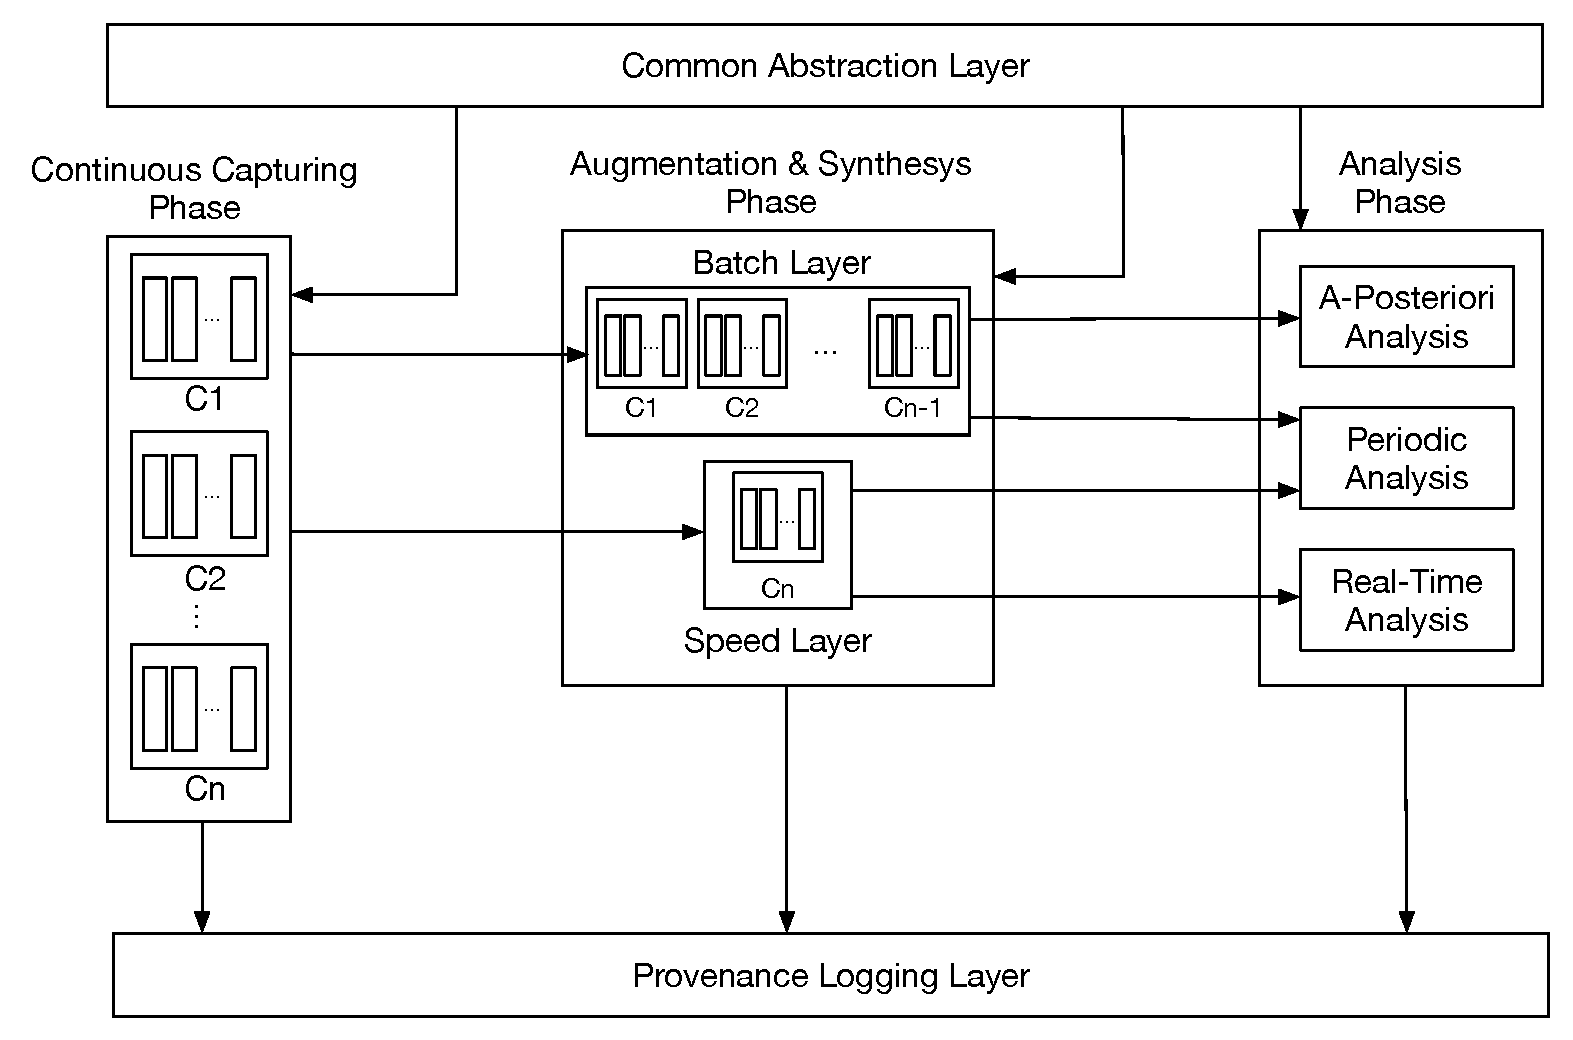
\includegraphics[width=\columnwidth]{img/computational-model-architecture}
    \caption{Example of the architecture of a system that implements \textnormal{\protect\river{}}.}
    \label{fig:arch}
\end{figure}

Figure~\ref{fig:arch} presents an reference architecture for systems that implement \river{} computational model. Information enters from the left and exits to the right going through three operational phases. 
Phase~1 (namely, Continuous Capturing Phase) continuously captures data over time. 
Phase~2 (namely, Augmentation and Synthesis Phases) enriches, manipulates and transforms captured data. 
Phase~3 (namely, Analysis Phase) analyses data to compute results.
Accordingly to the \river{}'s operators definition, Phase~1 exploits different implementations of the IN$\langle\mathrm{T}\rangle$ operator. 
Phase~2 exploits a combination of S2C$\langle\mathrm{T}\rangle$, C2C$\langle\mathrm{T},\mathrm{T^{\prime}}\rangle$ and C2S$\langle\mathrm{T}\rangle$ operators implementations. And, finally, Phase~3 exploits OUT$\langle\mathrm{T}\rangle$ operator implementations to emit the results.

During the Continuous Capturing Phase the data, which continuously flows in, is just marked with a timestamp, i.e., following the \textit{Lazy Transformation} approach, it is captured in its original form independently from its complexity.  

The proposed architecture treats \textit{Volume} as orthogonal to \textit{Variety} and \textit{Velocity}. When \textit{Volume} is present, system must implement the continuous ingestion phase in a partition tolerant way (see Section \ref{ch:computational-impl}). 

The fragment of the architecture, which has in charge the Augmentation and Synthesis Phases, is inspired by a $\lambda$ architecture (see Section~\ref{sec:vel-arch}). 
Let us denote with C$_i$ the information the Speed Layer is able to process while staying reactive, and let us denote with C$_n$ the most recently captured information, and with C$_1$, ..., C$_{n-1}$ all the data captured. While the Speed Layer processes C$_n$, the Batch Layer updates C$_1$, ..., C$_{n-2}$ with the results generated by the Speed Layer while processing C$_{n-1}$.

The Analysis Phase exploits, based on the information need of the user, indifferently various part of the upstream architecture. The Batch Layer can be used alone for periodic and post-hoc analysis, or in support of the Speed Layer for analysis that needs to compare the most recent data with the historical one. Nevertheless, the speed layer, can be independently used to perform instantaneous analysis.

For instance, a taxi company can exploit the Batch Layer, to synthesize statistics about the cost and the duration of all the rides captured so far in a city. An a-posteriori analysis of those statistics can determine a complete origin-destination matrix for the taxi rides, i.e., a distribution of the durations and the prices of all possible routes from any point to any other point in the city (see Section~\ref{sec:conc-fr-1-synth-ex}). At the same time, the taxi company can exploit the Speed Layer to determine the current most profitable routes using the latest incoming data. The comparison between the latest price of the rides (computed in the Speed Layer) with the information in the origin-destination matrix (computed in the Batch Layer) can be useful to foil a fraud.  

Two more layers compose the proposed architecture: the Common Abstraction Layer -- that contains the abstraction used to model or manipulate data (e.g., \frappe{} concepts and \river{}'s operators) and enables OBDA operations -- and the Provenance Logging Layer -- that contains all the artifact useful to document data lineage and to log the system actions (e.g., in accordance with concepts in the Provenance fragment of \frappe{}).

\section{Conclusion}
In this chapter, we investigate the problem of managing data characterized by high variety and velocity without forgetting volume.
Taking in account the conceptual model presented in Chapter~\ref{ch:conceptual}, we concentrate our efforts on the creation of a computational model to deal with data with such characteristics.

We propose \river{}, a variety-proof streaming computational model based on two main principles (see Section~\ref{sec:comp-mod-sol}): \textbf{(P1)} everything is a data stream, and \textbf{(P2)} Continuous Ingestion.
A system based on \textbf{(P1)} and \textbf{(P2)} can manage flowing data without any data loss.
During this research work, in order to answer the research question, we propose the \textit{Lazy Transformation} and formulate the hypothesis \textsf{Hp.2.1}.
A system, which implements the \textit{Lazy Transformation} approach, postpones the data transformation until it can benefit from it.

We present a formal definition of \river{}'s operators in terms of semantics and textual syntax (see Section~\ref{sec:comp-mod-sol-lang}), together with the Pipeline Definition Language (PDL) -- a graphic language that enables user to create computational plans, in the form of pipelines, to ingest, process and emit data.

\river{} represents the formal basis of the implementations proposed in the next chapter (see Chapter~\ref{ch:computational-impl}), that will be exploited to experimentally validate \textsf{Hp.2.1}. 
%Computational Model Implementations
\chapter{\texorpdfstring{\protect\river{}}{RIVER} Implementations and Evaluations}\label{ch:computational-impl}

\textcolor{red}{FINAL - TO BE READ ONE LAST TIME - READ FROM \ref{sec:comp-mod-eval-performace} ON}

In this chapter, we propose different implementations of \river{} computational model (see Chapter~\ref{ch:computational}) and the evaluations of such implementations from different points of view.
Section~\ref{sec:comp-mod-impl-intro} introduces the problem of implementing \river{} from the scalability perspective.
In Section~\ref{sec:comp-mod-impl} we propose \sti{} -- a vertically-scalable implementation of \river{} --, \sparkdi{} and \hivedi{} -- two horizontally-scalable implementations of \river{}.
The Section~\ref{sec:comp-mod-eval-performace} and the Section~\ref{sec:comp-mod-eval-cost} presents, respectively, the evaluation of \sti{} against an already existing system, and an evaluation of \sti{} against \sparkdi{} based on cost-effectiveness.

\section{Introduction and Problem Statement} \label{sec:comp-mod-impl-intro}
In the following sections, we discuss three alternative implementations of \river{} computational model.
Based on our experiences, we identify three situations where the nature of the data, in particular the \textit{Volume}, and the system scalability requirements shape the specific implementation of \river{} reference architecture (see Section~\ref{sec:comp-mod-sol-arch}).
In particular, inspired by the benchmarking basic principles (see Section~\ref{sec:benchmarking}), we consider the \textit{cost effectiveness} as the most important characteristic of an implementation.

When the amount of data is small and the cost of a complex infrastructure is unaffordable, an ad-hoc implementation results suitable.
In this situation, there is no need for scalability and the final artifact can be developed in any language or using any framework, e.g. Python or Java.
We work following this direction~\cite{BalduiniJBD2018}, but we do not report the results because they are out of the scope of this thesis.
If the amount of data grows, a scalability requirement arises. An ad-hoc solution results hard to be cost-effective, if compared to a more generic and reusable implementation. 

Conscious that distribution and parallelization does not pay at all scales~\cite{bodendistributed}, we developed (i) a vertically scalable single threaded implementation -- \sti{} -- and (ii) two horizontally scalable implementations based on Spark -- \sparkdi{} -- and Hive -- \hivedi{}.
In the next sections, we present \sti{}, \sparkdi{} and \hivedi{}, and the evaluation results that validated the Hypothesis \textsf{Hp.2.1} (formulated in Chapter~\ref{ch:computational}).

Moreover, in order to cast some light on the research questions taking in account possible alternative implementations, w.r.t. scalability, we formulate the hypothesis: 
\begin{itemize}[leftmargin=42pt]
\item[\textsf{Hp.2.2}] A single-threaded implementation of the streaming computational model from \textsf{Hp.2.1} is more cost-effective than a distributed implementation of the same model while guaranteeing the reactiveness of the system.
\end{itemize}

\section{Implementations} \label{sec:comp-mod-impl}
Section~\ref{sec:comp-mod-impl-v} proposes \sti{}, an implementation based on single-threaded technology able to manage heterogeneous streaming data characterized by medium Volume.
When scaling to large volume is required, a single threaded implementation is at risk of loosing cost-effectiveness because, even if the entry cost is much lower than a Big Data implementation, its cost grows exponentially in the size of the data. Therefore, an horizontally scalable solution, using Big Data technology, represents a good choice.
The results of the evaluation reported in Section~\ref{sec:comp-mod-eval-performace}, convinced us to assume the \textsf{Lazy Transformation} as a principle to be applied in the horizontally scalable implementations of \river{} computational model.
In our work, we employed two different solutions respectively based on Spark (\sparkdi{}) and Hive (\hivedi{}).
Section~\ref{sec:comp-mod-impl-h-spark} and Section~\ref{sec:comp-mod-impl-h-hive} present an overview of those implementations.

\subsection{\sti{} - A Vertically Scalable Implementation} \label{sec:comp-mod-impl-v}
\sti{} is a single threaded implementation of \river{} reference architecture (see Section~\ref{sec:comp-mod-sol-arch}) able to deal with continuously flowing data characterized by medium Volume, high Variety and very high Velocity. 
It continuously ingests streaming data represented as a time-stamped data items that are typed, only when needed. The type is declared as an annotation to the captured information.

\begin{figure}[t]
\centering
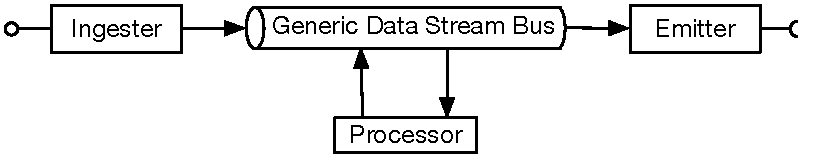
\includegraphics[width=0.9\textwidth]{img/comp-mod-natron-schema}
\caption{Overview of \sti{} architecture.}
\label{fig:sti}
\end{figure} 

Figure~\ref{fig:sti} depicts an overview of the \sti{} internals.
The Ingesters allow ingesting external data flows, and push the data on the Generic Stream Bus.
As recommended by the \textit{Lazy Transformation} approach, we postpone the transformation as long as possible in the process, only the ingestion time is added. 
The Processors, e.g. an Information Flow Processor as Esper (see Section~\ref{sec:esper-epl}), listens to one or more streams S$\langle\mathrm{T}\rangle$, computes different operations and produces a new stream S$^{\prime}\langle\mathrm{T^{\prime}}\rangle$. 
Emitters allow \sti{} producing a new external data flow in multiple formats. 
In \sti{}, the window operator can be implemented in two different ways: either using the ingestion timestamp added during the Continuous Capturing Phase, or using an application timestamp, e.g. a time mark added during the Augmentation \& Synthesis Phase referring to the notion of Frame in \frappe{}.

\subsection{\protect\sparkdi{} - A Horizontally Scalable Implementation Based on Spark} \label{sec:comp-mod-impl-h-spark}

\sparkdi{} is an implementation of \river{} based on Spark Structured Streaming processing engine (see Section~\ref{sec:spark}). 
It enables the users to create pipeline of streaming computation as they are creating a batch computation, and to leave to the Spark SQL engine to manage the incremental update of the results in a transparent way.

\sparkdi{} offers different implementations of the IN$\langle\mathrm{T}\rangle$ operator that exploits the DataFrames and Datasets API offered by Spark to ingest data from different sources (e.g., filesystem, Kafka, socket, etc.).
In the same way, \sparkdi{} exploits the sink of Spark Structured Streaming as implementations of the OUT$\langle\mathrm{T}\rangle$ operators (e.g., filesystem sink, Kafka sink, Console sink, etc.).
The access to the data, during the Ingestion and Augmentation \& Synthesis Phase,  is guaranteed by OBDA techniques implemented in the various components that exploit \frappe{} as data schema.
Moreover, the Dataframe APIs enable the implementation of all the \river{}'s operators and allow the development of the complete stack of layers presented in the \river{} reference architecture (see Section~\ref{sec:comp-mod-sol-arch}).

\begin{figure}[ht]
\begin{minipage}{0.95\linewidth}
\begin{lstlisting}[caption={Example of Window operator in Spark.},label=lst:spark-ex,style=SPARKCODE]
   val itemsCounts = inputStream.groupBy(
        window($"ts", "40 seconds", "20 seconds"),
        $"Agg(Count)"
     ).count()
\end{lstlisting}
\end{minipage}
\end{figure}

In particular, the \sparkdi{} implementation of the S2C$\langle\mathrm{T}\rangle$ window operator exploits the native Spark Structured Streaming windowing operations on the ingestion time added to the data during the Continuous Capturing phase.

{Listing~\ref{lst:spark-ex} presents the code to compute the aggregation \textit{Agg(Count)}, representing the amount of the data items that entered the system in the last 40 seconds, using a window that slides every 20 seconds.

\subsection{\protect\hivedi{} - A Horizontally Scalable Implementation Based on Hive} \label{sec:comp-mod-impl-h-hive}
\hivedi{} is a distributed implementation of \river{} computational model based on Hive (see Section~\ref{sec:hive}).
Hive is a Big Data warehouse solution and is not originally ready for managing streaming data.
This limitation can be overcome by chaining, during the Ingestion Phase, the implementations of a IN$\langle\mathrm{T}\rangle$ operator and a S2C$\langle\mathrm{T}\rangle$ operator (window). This chain enable the system to add the ingestion timestamp, \textit{ts} to each incoming data and to transform the time-varying input into a Hive compatible static format (e.g., Parquet) partitioned by \textit{ts}. 
The Augmentation \& Synthesis Phase exploits OBDA techniques to access data using \frappe{} ontology as data schema.
The \frappe{} Commons Abstractions layer contains the concepts to enrich and transform data according to the \frappe{} conceptual model (e.g., adding a reference to \frappe{} Frame that groups the data items by time and space).
The final result is then served to the user through implementations of different OUT$\langle\mathrm{T}\rangle$ operators that allow the system to save the data in different format (e.g., filesystem, Kafka, websocket).

As for the \sparkdi{}, we now focus on the S2C$\langle\mathrm{T}\rangle$ window operator in \hivedi{} that exploits the Hive window operator. Differently from Spark, the window operator is not natively supported due to the batch nature of the framework. However, if we augment the data items with a frame ID during the Augmentation \& Synthesis Phase, tumbling windows can be implemented grouping by Frame ID. 

\begin{figure}[ht]
\centering
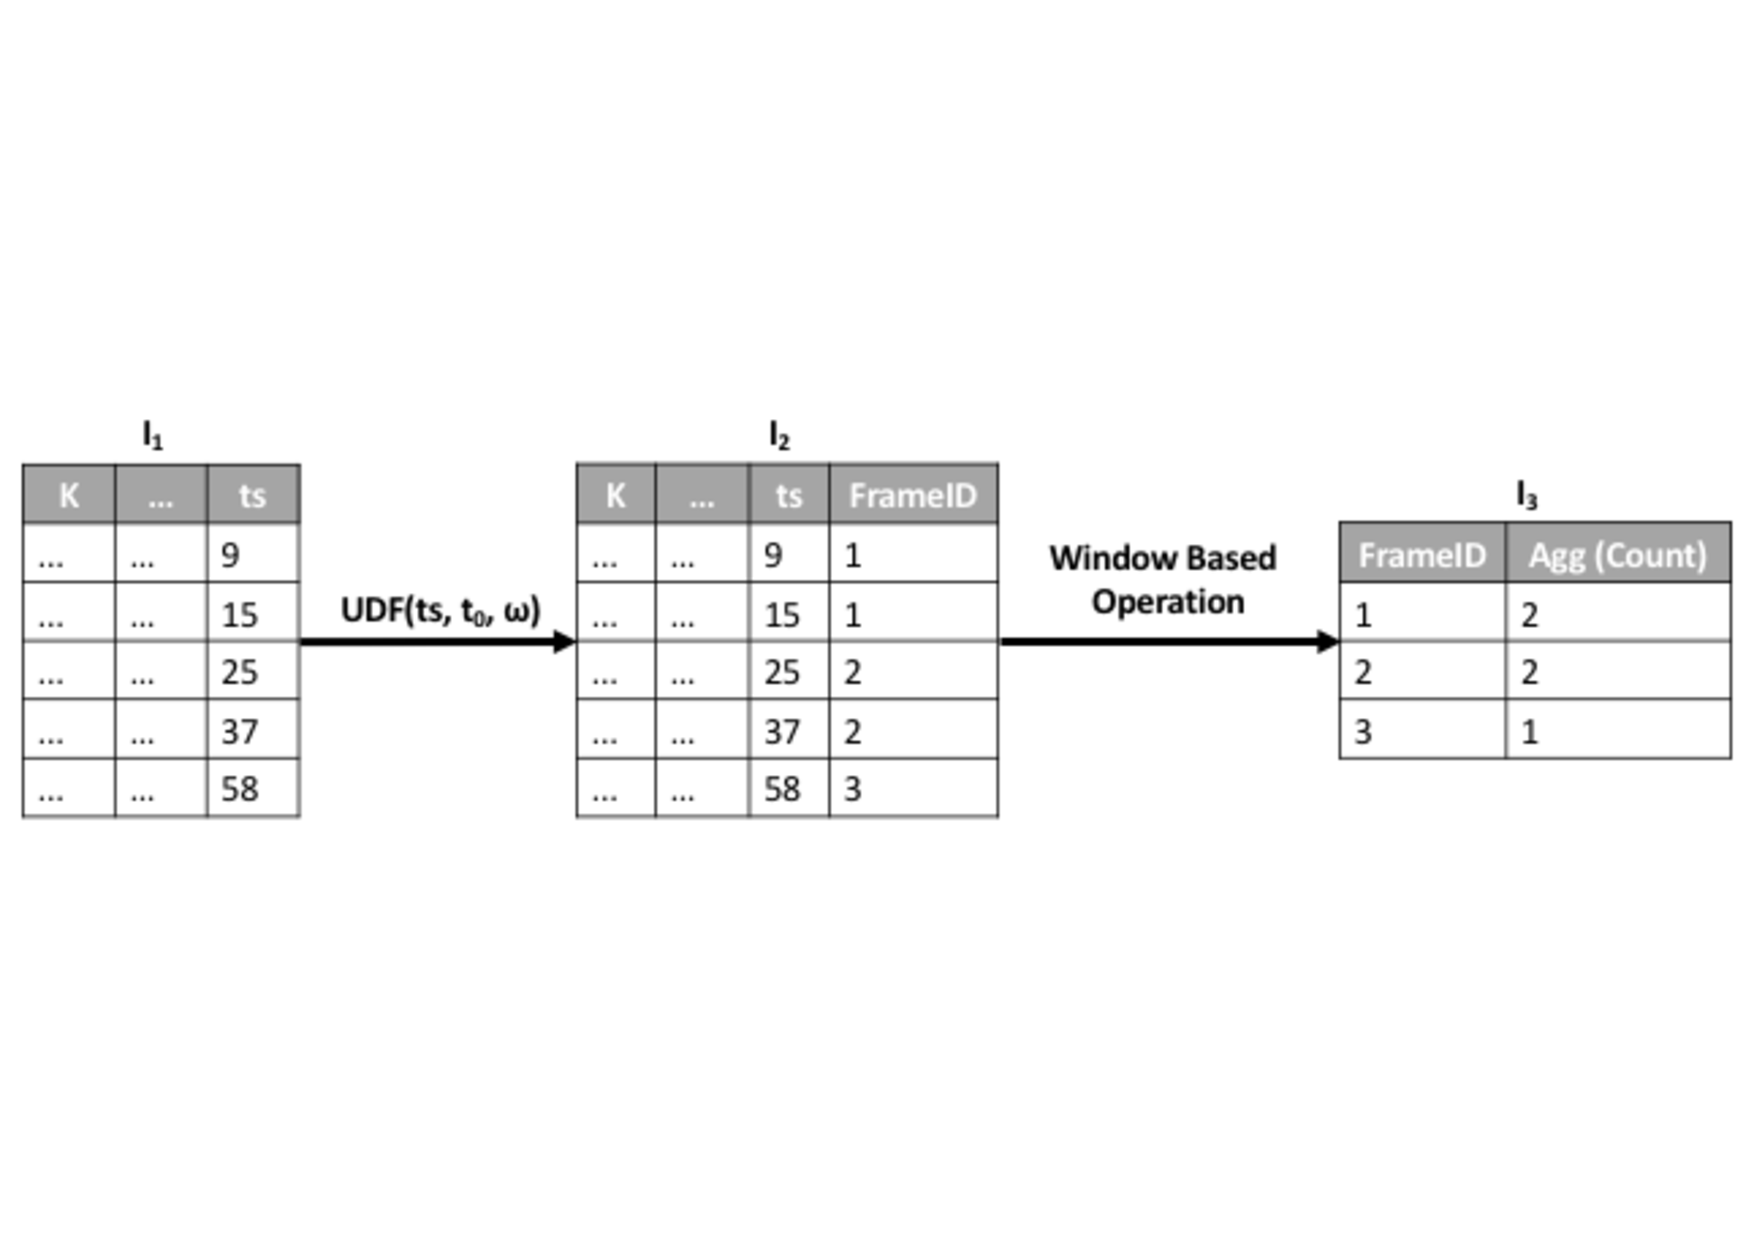
\includegraphics[width=0.92\textwidth]{img/hive_example}
\caption{Example of Window operator using Hive.}
\label{fig:hive-ex}
\end{figure} 

Figure~\ref{fig:hive-ex} shows a simple example of a chain of operations that ingest a data stream, augment it with a Frame ID and simulates a tumbling window that counts the number of data items per frame. \textit{I$_1$} represents the data saved on HDFS during the ingestion phase. \textit{I$_1$} is in form of a table containing various attributes and partitioned by the ingestion timestamp \textit{ts}. The data is augmented using a query that uses a User Defined Function (UDF) to attach a Frame ID based on the \textit{ts} and save the result incrementally in a parquet file partitioned by Frame ID. Such an UDF is configured passing the opening time t$_0$ of the first window, and the length of a Frame  $\omega$. In the example t$_0$ = 0 and $\omega$ = 20. The Frame groups the data items in windows and enables operation on time-varying data in a batch oriented system such as Hive. \textit{I$_2$} represents the augmented data. The Window Based Operation exploits the Frame ID to perform a simple count aggregation by applying a Group by on the Frame ID.  \textit{I$_3$} represents the aggregated data.

\section{Validation of the Lazy Transformation Approach} \label{sec:comp-mod-eval-performace}

As a first evaluation step, we compared \sti{} against SLD (see Section~\ref{sec:rsp-mid}). Both of them are single-threaded but, while SLD is based on RDF streams, \sti{} implements the \textit{Lazy Transformation} approach.

Differently from SLD, \sti{} i) uses time-stamped generic data items (instead of focusing only time-stamped RDF graphs) and ii) processes them according to their original nature.
In particular, we test if a system exploiting i) and ii) results a cheaper (using less memory and CPU), faster (reaching higher maximum input throughput) and more accurate (better approximating the correct answer) version of a streaming computational model.

In the following sections, we expose the problem, the solution design and the experimental settings, and, finally, we bring experimental evidences that validate the hypothesis \textsf{Hp.2.1}.

\subsection{Problem Settings}
As domain, we chose Social Media analysis as done by the Linked Data Benchmark Council (LDBC) in the SNBench\footnote{\url{http://www.ldbcouncil.org/benchmarks/snb}}. 

SLD and \sti{} receive information in the same way, they both connect to a web socket and handle JSON-LD files. 

\begin{figure}[ht]
\begin{minipage}{0.95\linewidth}
\begin{lstlisting}[caption={JSON representation of a Twitter micro-post. Due to the lack of space we omitted the context declaration that contains the namespace.},label=lst:json-post, style=JSON]
{"@context": { ... }, 
  "@type": "Collection",
  "totalItems": 1,
  "prov:wasAssociatedWith": "sr:Twitter",
  "items": [{
    "@type": "Post",
    "published": "2016-04-26T15:40:03.054+02:00",
    "actor": {
      "@type": "Account",
      "@id": "user:1",
      "sioc:name": "@streamreasoning"
    },
    "object": {
      "@type": "Content",
      "@id": "post:2",
      "alias": "http://.../2",
      "prov:wasAssociatedWith": "sr:Twitter",
      "sioc:content": "You ARE the #socialmedia!",
      "dct:language": "en",
      "tag": [{
        "@type": "Tag",
        "@id": "tag:3",
        "displayName": "socialmedia"
      }]
    }
  }]
}
\end{lstlisting}
\end{minipage}
\end{figure}

In Listing \ref{lst:json-post}, we propose a JSON-LD serialization of the Activity Stream\footnote{\url{https://www.w3.org/TR/activitystreams-core/}} representation of a tweet as it was injected during the experiments in both systems.  
The JSON-LD representation of an Activity Stream is a \textit{Collection} (specified by \textit{@type} property) composed by one or more social media items. The \textit{Collection} is described by two properties, i.e., \textit{totalItems} and \textit{prov:wasAssociatedWith}, which tell respectively the number of items and the provenance of the items. The collection in the example contains a \textit{Post} created on \textit{2016-04-26} (\textit{published} property) by  an \textit{actor} (Line 6) that produce the \textit{object} (Lines 7-13). 
The \textit{Actor} has a unique identifier  \textit{@id}, a \textit{displayName}, a \textit{sioc:name} and a \textit{alias}. The \textit{Object} has a \textit{sioc:content}, a \textit{dct:language}, zero or more \textit{tag}s, and optionally a \textit{url} and a \textit{to} to represent, respectively, links to web pages and mentions of other actors.

\begin{figure}[ht]
\begin{minipage}{0.95\linewidth}
\begin{lstlisting} [caption={RDF N3 representation of a Twitter micro-post},label=lst:rdf-post, style=N3]
<post:2> a sma:Tweet ;
  dcterms:created "2016-04-26T15:40:03.054+02:00"^^xsd:dateTime ;
  dcterms:language "en"^^xsd:string ;
  sioc:content "You ARE the #socialmedia!"^^xsd:string ;
  sioc:has_container "Twitter"^^xsd:string ;
  sioc:has_creator <user:1> ;
  sioc:id "2"^^xsd:string ;
  sioc:link "http://.../status/2"^^xsd:string ;
  sioc:topic <tag:3> .
<tag:3> a sioct:Tag ;
  rdfs:label "socialmedia"^^xsd:string .
<user:1> a sioc:UserAccount ;
  sioc:account_of "StreamReasoning"^^xsd:string ;
  sioc:creator_of <post:2> ;
  sioc:id "1"^^xsd:string ;
  sioc:name "@streamreasoning"^^xsd:string .
\end{lstlisting}
\end{minipage}
\end{figure}

Listing~\ref{lst:rdf-post} shows the RDF produced by SLD in transforming the JSON-LD in Listing~\ref{lst:json-post} at ingestion time. The translation exploits well known vocabularies, in particular SIOC\footnote{\url{http://sioc-project.org/}} to represent the online community information, PROV-~O~\cite{w3c-prov-o} to track the provenance of an item and DCTERMS\footnote{\url{http://dublincore.org/documents/dcmi-terms/}} to represents information about the \textit{object}.

\subsection{Solution Design and Experimental Settings} 
A test consists of sending a constant amount of JSON-LD synthetic data.
The data is sent in chunks three times per minute (i.e. at the 10$^{th}$, the 30$^{th}$ and the 50$^{th}$ seconds of the minute).  Each chunk contains the same amount of posts. We tested the configuration for different rates: 1500 posts per minute (i.e., three chunks of 500 posts), 3000 posts per minute, 6000 posts per minute, 9000 posts per minute, 12000 posts per minute and 18000 posts per minute.

The rates and the input methodology test a normal situation for SLD (1500 and 3000 posts per minutes) as well as situations that we know to overload SLD (more than 6000 posts per minute)~\cite{DBLP:conf/esws/BalduiniV017a}.

\begin{figure}[t]
\centering
\subfloat[]{
	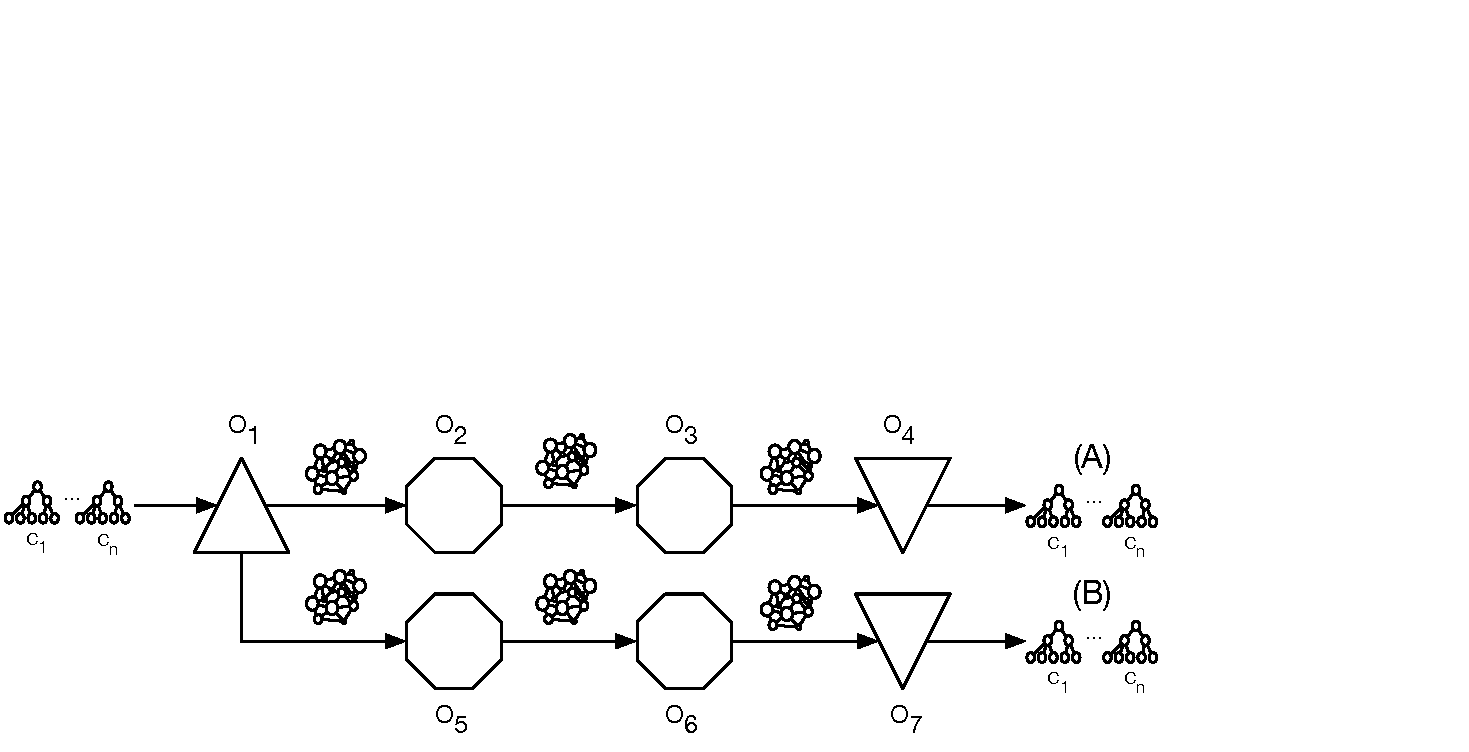
\includegraphics[width=0.8\textwidth]{img/comp-mod-sld-pipeline}
	\label{fig:sld-pl}
} \\
\subfloat[]{
	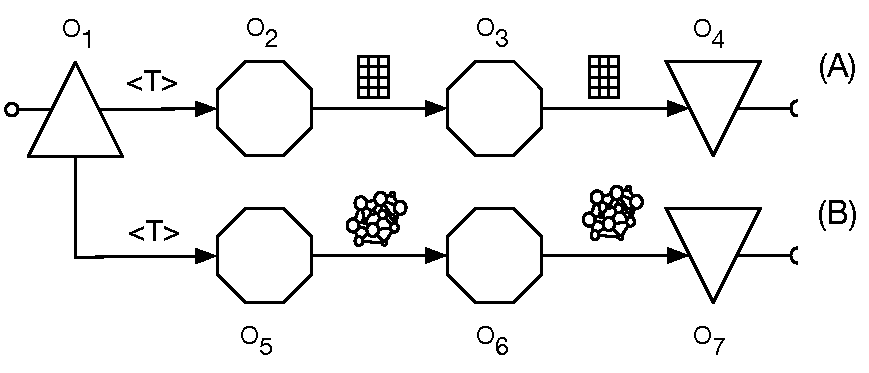
\includegraphics[width=0.8\textwidth]{img/comp-mod-natron-pipeline}
	\label{fig:natron-pl}
}
\caption{(a) SLD pipeline. Even if both the input and the output data are in JSON-LD format, SLD use RDF graph for the internal computation.
(b) \sti{} pipeline. The input and the output data are both in JSON-LD format, \sti{} keeps the data in tree format as long as possible during the internal computation.
Both the pipelines are presented exploiting the Pipeline Definition Language (see Chapter~\ref{ch:computational})}
\end{figure}

the pipelines used for testing the systems (depicted in Figure~\ref{fig:sld-pl} and in Figure~\ref{fig:natron-pl}) are both split into two branch. The first branch produces an \textit{area chart} by computing the number of tweets observed over time, the second one produces a \textit{bar chart} by counting how often hashtags appear in the tweets received in the last 15 minutes.

The two pipelines are coded in SLD and \sti{} in two different ways. 
SLD performs the transformations of JSON-LD in RDF by default, on all the input data, independently from the task to perform. \sti{} keeps the data in its original format as much as possible, i.e., it implements the \textit{Lazy Transformations} approach.
In \sti{}, the results can be continuously computed \textit{i}) using a generic sliding window S2C$\langle Tree \rangle$ operator, which works looking only to the time-stamps of the data items in the generic stream, and \textit{ii}) accessing with C2C$\langle Tree \rangle$ operator implemented as a path expression the \textit{totalItems} property in the JSON-LD file, i.e., the number of items in the collection.

Figure~\ref{fig:sld-pl} presents the two pipelines in SLD with PDL.
The input data are translated in RDF as soon as they enter the pipelines by the \textsf{Ingester} O$_1$, an implementation of an IN$\langle\mathrm{T}\rangle$ operator. The computations for the area chart and for the bar chart (see the part marked with \textbf{A} and \textbf{B} ) are composed by the same type of components and share the new RDF stream translated by O$_1$.
The pipeline \textbf{A} uses two C-SPARQL queries applied to the stream by the operators O$_2$ and O$_3$. Both of them represent a chain of 3 different \river{} operators (a S2C$\langle\mathrm{T}\rangle$, a C2C$\langle\mathrm{T},\mathrm{T}'\rangle$ and a C2S$\langle\mathrm{T}'\rangle$). 
O$_2$ (see Listing~\ref{lst:csparql-prequery}) applies a tumbling window of 1 minute, while O$_3$ aggregates the results using a 15 minutes time window that slides every minute (see Listing~\ref{lst:csparql-query}). 

\begin{figure}[ht]
\begin{minipage}{0.95\linewidth}
\begin{lstlisting} [caption={C-SPARQL query applied by O$_2$ that count the number of post in the stream from O$_1$ using a tumbling window of 1 minute.},label=lst:csparql-prequery, style=CSPARQL]
REGISTER STREAM presocialstr AS 
CONSTRUCT { ?id sma:twitterCount ?twitterC } 
FROM STREAM <http://.../socialstr> [RANGE 1m STEP 1m] 
WHERE { 
    SELECT (uuid() AS ?id) ?twitterC 
    WHERE { 
        SELECT (COUNT (DISTINCT ?mp) AS ?twitterC) 
        WHERE { ?mp a sma:Tweet } 
    } 
}
\end{lstlisting}
\end{minipage}
\end{figure}

\begin{figure}[ht]
\begin{minipage}{0.95\linewidth}
\begin{lstlisting} [caption={C-SPARQL query applied by O$_3$ that aggregates the results from O$_2$ using a 15 minutes time window that slides every minute.},label=lst:csparql-query, style=CSPARQL]
REGISTER STREAM ac AS 
CONSTRUCT { ?uid sma:twitterCount ?totTwitter ; 
              sma:created_during ?unixTimeFrame 
          } 
FROM STREAM <http://.../presocialstr> [RANGE 15m STEP 1m] 
WHERE { 
  SELECT (uuid() AS ?uid) 
         ?unixTimeFrame 
         (SUM(?twitter) AS ?totTwitter)
  WHERE { ?id sma:twitterCount ?twitter ; 
            sma:created_during ?timeFrame . 
          ?timeFrame a sma:15mTimeFrame ; 
            sma:inUnixTime ?unixTimeFrame  
        } 
  GROUP BY ?unixTimeFrame 
}
\end{lstlisting}
\end{minipage}
\end{figure}

It is worth to note that the first query is an important optimization in terms of memory consumption. It avoids the engine to keep 15 minutes of tweets only to count them. In SLD, we often use this design pattern, we call this first query a \textit{pre-query}.
Pipeline \textbf{B} also exploits this design; it applies a pre-query through the O$_5$ operator to reduce the amount of data and, then, a query to produce the final result through the O$_6$ operator. 
It is also worth to note that all the C-SPARQL queries use the form REGISTER STREAM ... AS CONSTRUCT ..., because RDF streams are the only means of communication between SLD components.
The OUT$\langle\mathrm{T}\rangle$ operators of both pipelines, namely O$_4$ and O$_7$, make the results available to processes outside SLD. In this case, both O$_4$ and O$_7$, write JSON files on disk.

Figure~\ref{fig:natron-pl} presents the pipelines in \sti{}. As for SLD, the pipeline \textbf{A} is for the area chart, while \textbf{B} is for the bar chart. 
Differently from the \textsf{Ingester} in the SLD pipeline, O$_1$ does not apply any transformation to the input stream, and the data flows in \sti{} in JSON-LD format.
The O$_1$ operator applies a generic EPL query (presented in Listing~\ref{lst:epl-query}) characterized by a 1 minute long time window.
The clauses \texttt{FORCE\_UPDATE}\footnote{The FORCE\_UPDATE flow control keyword instructs the view to post an empty result set to listeners if there is no data to post for an interval. Note that FORCE\_UPDATE is for use with listeners to the same statement and not for use with named windows. Consider output rate limiting instead.} and \texttt{START\_EAGER}\footnote{The START\_EAGER flow control keyword instructs the view to post empty result sets even before the first event arrives, starting a time interval at statement creation time. As when using FORCE\_UPDATE, the view also posts an empty result set to listeners if there is no data to post for an interval, however it starts doing so at time of statement creation rather then at the time of arrival of the first event.} tell the stream processing engine, respectively, to emit also empty reports and to start processing the window as soon as the query is registered (i.e., without waiting for the first time-stamped data item to arrive).
It is worth to note that this query exploits the event-based nature of the generic stream it is observing.
It does not inspect the payload of the events; it only uses their time-stamps.

\begin{figure}[ht]
\begin{minipage}{0.95\linewidth}
\begin{lstlisting} [caption={The generic window query applied by the operator O$_1$.},label=lst:epl-query,numbers=none, style=ESPER]
SELECT * 
FROM event#TIME(1 min,"FORCE_UPDATE, START_EAGER")
\end{lstlisting}
\end{minipage}
\end{figure}

As explained in Section~\ref{sec:comp-mod-impl-v}, processors are the central components of \sti{}. They can listen to one or more generic stream, compute different operations and push out a generic streams. The type of the input and output streams can be different. The two pipelines use different processors (e.g. RDF translator, windower and SPARQL).

\sti{} maintains the data format as long as possible in order to reduce the overhead of the translations. It can exploit the tree-based nature of JSON-LD. In pipeline \textbf{A}, the operator O$_3$ exploits a path expression data to extract \textit{totalItems}, i.e., the number of items in each collection, from the time-stamped JSON-LD items in the generic stream it listens to. It outputs a tuple $\langle$timeframe,count$\rangle$ that is aggregated every minute over a window of 15 minutes using an EPL statement.

The pipeline \textbf{B} of \sti{} shares the O$_1$ operator with the pipeline \textbf{A}.
The operator O$_5$ translates the generics in input in RDF graph. This transformation is required to extract information about the hashtags. As for the pipeline \textbf{B} of SLD, we use a pre-query design pattern to reduce the amount of data. A SPARQL processor, implementing the operator O$_5$, applies the SELECT query in Listing~\ref{lst:sparql-prequery} to every data-item in the stream and pushes out a stream of tuples $\langle$hashtagLabel,count$\rangle$. The relational stream is then aggregated with an ESPER processor, which implements O$_6$, with a 15 minute time window that slides every 1 minute (see Listing~\ref{lst:epl-query-bc}). 

\begin{figure}[ht]
\begin{minipage}{0.95\linewidth}
\centering
\begin{lstlisting} [caption={SPARQL pre-query applied by the component O$_6$},label=lst:sparql-prequery, style=SPARQL]
SELECT ?htlabel (COUNT(DISTINCT(?mpTweet)) AS ?htTweetCount) 
WHERE { ?mpTweet a sma:Tweet ; sioc:topic ?tweetTopic . 
        ?tweetTopic a sioctypes:Tag ; rdfs:label ?htlabel } 
GROUP BY ?htlabel 
ORDER BY DESC(?htTweetCount) 
\end{lstlisting}
\end{minipage}
\end{figure}

\begin{figure}[ht]
\begin{minipage}{0.95\linewidth}
\begin{lstlisting} [caption={EPL query for the bar chart, applied to the stream by the component O$_6$},label=lst:epl-query-bc,numbers=none, style=ESPER]
SELECT htlabel, SUM(count) as sumHt 
FROM HTCountEvent#TIME(15 min) 
GROUP BY htlabel 
OUTPUT SNAPSHOT EVERY 1 min 
\end{lstlisting}
\end{minipage}
\end{figure}

As for SLD pipelines, the operators O$_4$ and O$_7$ of the \sti{} pipelines are implementations of \textsf{Emitter}s and offer the result to the user in the form of JSON files on disk.

\subsection{Results and Discussion}\label{sec:comp-mod-eval-performace-res}
As key performance indicators (KPIs), we measure  the resources consumption of the two systems and the correctness of the results. For the resource consumption, we measure every 10 seconds: \textit{i}) the CPU load of the system thread in percentage, \textit{ii}) the memory consumption of the thread in MB and \textit{iii}) the memory consumption of the Java Virtual Machine (JVM). For the correctness, we compared the computed results with the expected results. Being the input a constant flows of tweets that only differ for the ID, the area chart is expected to be flat and the bar chart is expected to count exactly the same number of hashtags every minute.

\begin{figure}[t]
\centering
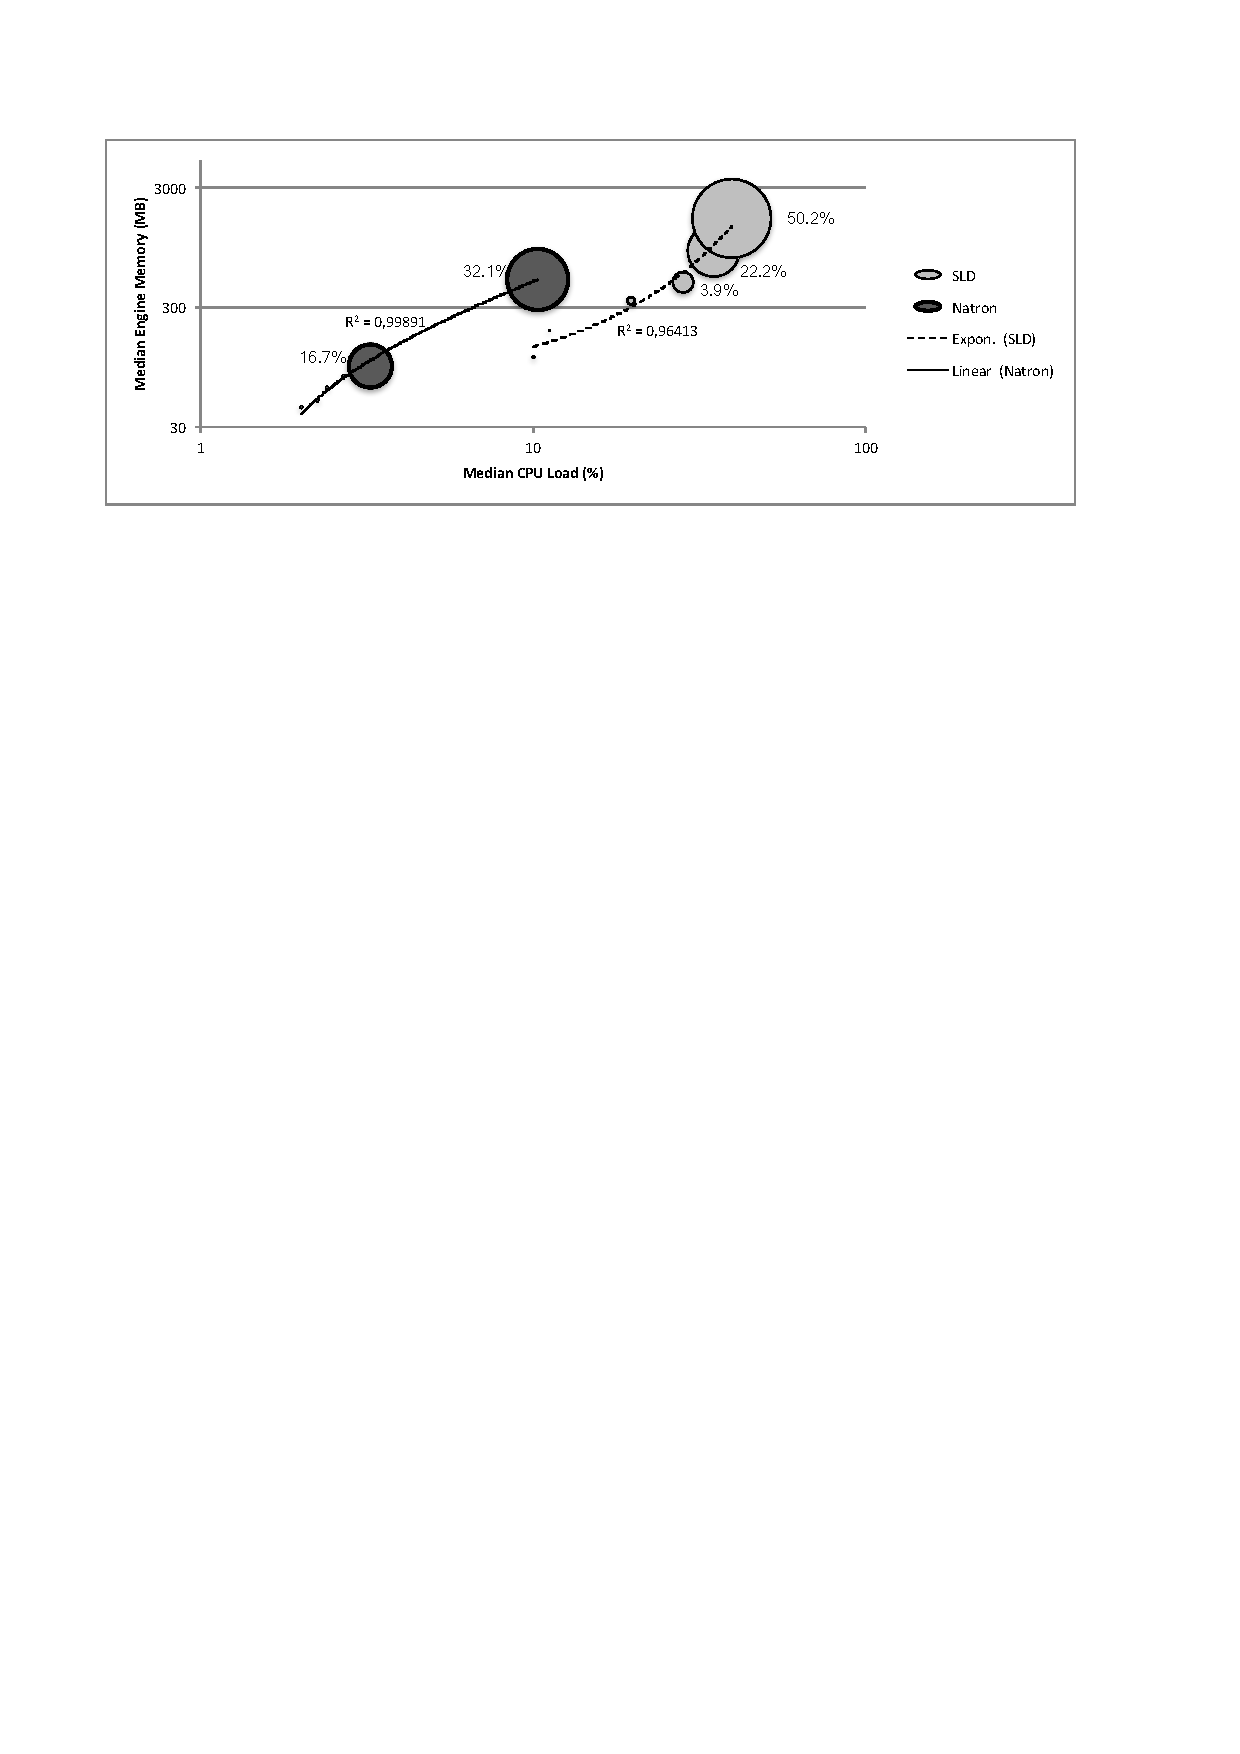
\includegraphics[width=\textwidth]{img/comp-mod-cpu-mem-acerror}
\caption{An overview of the experimental results; larger  bubbles means greater \% errors.}
\label{fig:cpu-mem}
\end{figure}

\begin{figure}[t]
\centering
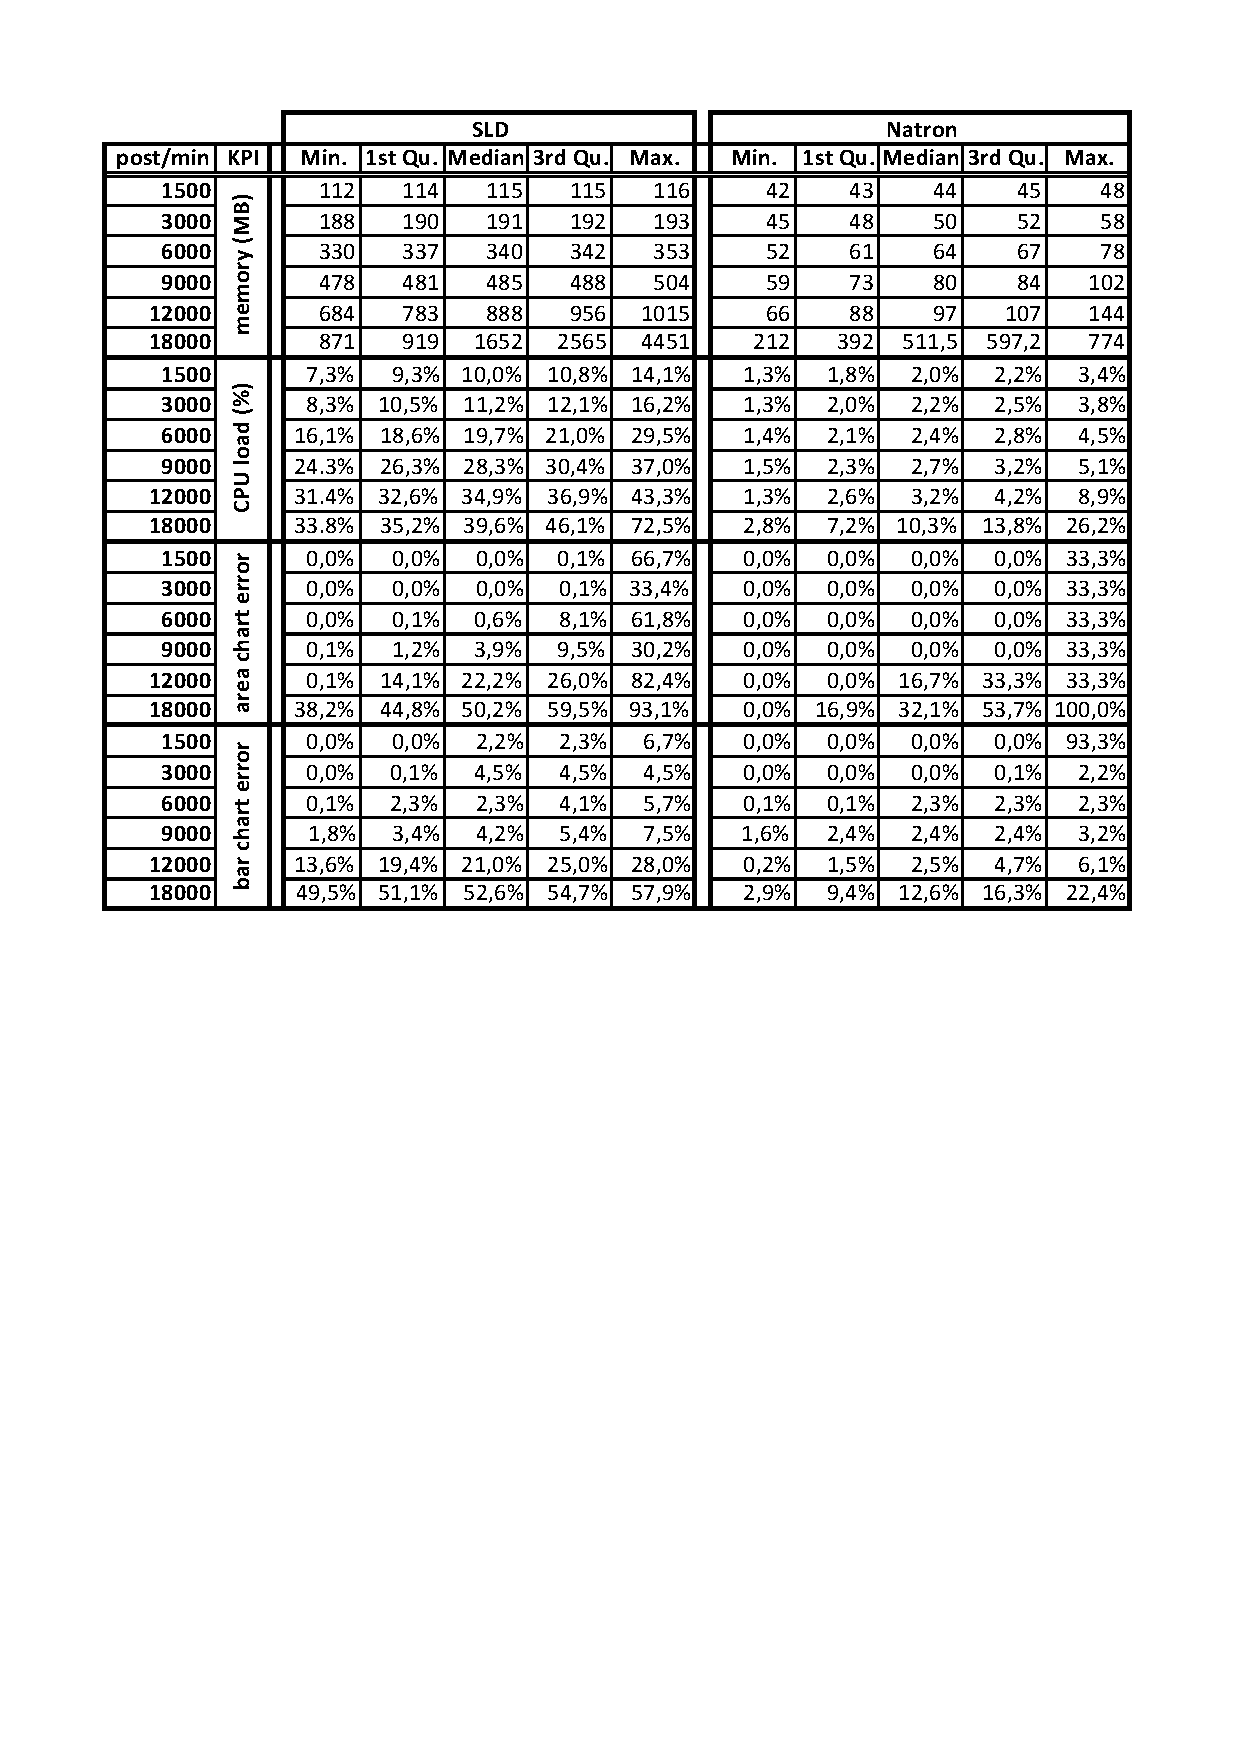
\includegraphics[width=\textwidth]{img/comp-mod-results}
\caption{The experimental results.}
%\vspace{-0.5cm}
\label{fig:all-data}
\end{figure}

Figure~\ref{fig:cpu-mem} offers an overview of the results of the experiments. The full results are reported at the end of this section in Figure~\ref{fig:all-data}. On the X, axis we plot the median of the CPU load in percent, while on the Y axis, we plot the memory allocated by the engine thread. The size of the bubble maps the median of the error of the area chart. Bubbles in the lower left corner correspond to the experiment where we sent 1500 tweets per minute.

Increasing the throughput results in more memory consumption and CPU load for both systems. However, \sti{} consumes less memory than SLD and occupies less CPU. Moreover, \sti{} presents a linear increment for both these KPIs, while the resource usage for SLD grows exponentially with the throughput (note the R$^2$ in Figure~\ref{fig:cpu-mem}). Also the error in the results increases with the throughput: SLD already shows an median error greater than 3\% in the bar chart at 3000 tweets per minutes and in the area chart at 9000 tweets per minute; \sti{} is faster - i.e. it reaches higher maximum input throughput - and more accurate -- i.e. it reaches 3\% error level only for 18000 tweets per minutes, providing more precise results than SLD.

Figure~\ref{fig:timeplots} presents the recorded time-series for CPU load and memory usage in both systems. The memory usage graphs contain two different time series. The blue one represents the memory usage of the system thread, while the orange one shows the total memory usage for the JVM.

\begin{figure}[p]
\centering
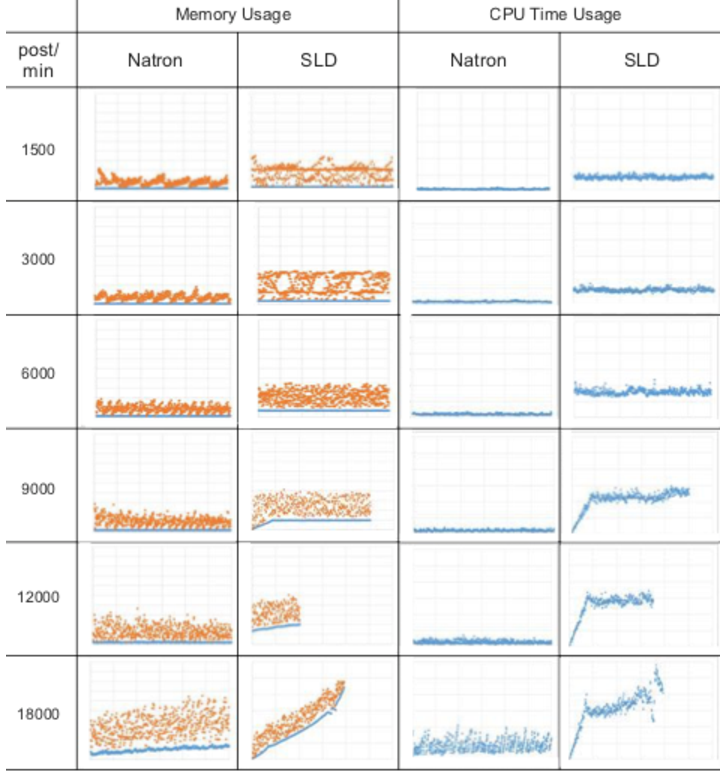
\includegraphics[width=\textwidth]{img/comp-mod-timeplots}
\caption{Memory and CPU usage over time. In the Memory Usage columns, the blue dots represents the memory usage of the system thread, while the orange dots shows the total memory usage for the JVM. In the CPU Time Usage columns, the blue dots represents the CPU time usage of the system thread.}
\label{fig:timeplots}
\end{figure}

The memory usage of the system thread accounts for all the components and data in the pipeline. Notably, when the system under testing is not overloaded, the memory usage is constant over time, while when the system is overloaded it grows until the system crashes. The total memory usage of the JVM shows, instead, the typical pattern of the garbage collector that lets the JVM memory grow before freeing it. Also in this case, when the system it is overloaded, the garbage collector fails to free the memory.

During the experiments the median of the  memory used by SLD spans from 115 MB, when loaded with at 1500 posts/min, to 1.6 GB, when loaded with 18000 posts/min. For \sti{}, instead, it spans from 44 MB to 511.5 MB in the same load conditions. The experimental results clearly shows that \sti{} consumes (in average) three times less memory than SLD.

\begin{figure}[p]
\centering
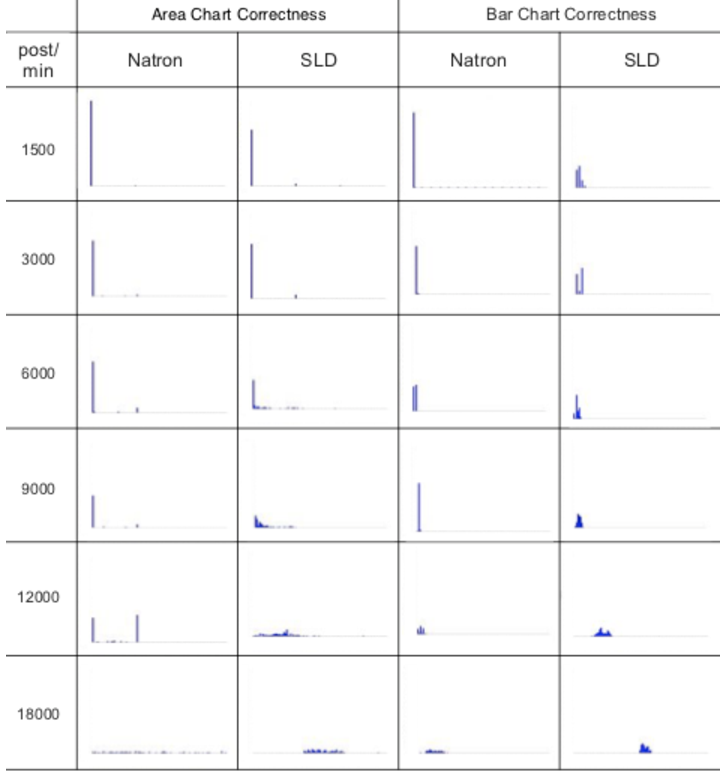
\includegraphics[width=\textwidth]{img/comp-mod-errors}
\caption{Area chart and bar chart errors distributions}
\label{fig:errors}
\end{figure}

The same considerations can be proposed for the CPU load. The median of the CPU load spans  from 2\% to 10\% for \sti{}, while it spans from 10\% to 39.5\% for SLD. \sti{} consumes in average 4 time less CPU time than SLD. 
Moreover, it offers higher level of stability for both the parameters in all the experiments. 

The correctness results are summarized in Figure~\ref{fig:errors}. The X axis of each plot shows the percentage of error; it ranges from 0\% to 100\%. The Y axis is the percentage of results with that error; it also ranges from 0\% to 100\%. A bar as tall as the Y axis in the left side of the graph means that all results where correct. The smaller that bar is and the greater the number of bars to the right is, the more errors were observed.

In general, the results show that \sti{} is more accurate (the result error is smaller) than SLD and, consequently, validate the hypothesis \textsf{Hp.2.1}. For the area chart the distribution shows that \sti{} percentage of error is very low when the input throughput is between 1500 posts/min and 9000 posts/min. When it is higher (i.e., 12000 and  18000 posts/min) also \sti{} starts suffering and the percentage of errors starts growing. For SLD, errors are present even at lower input rate, the graph shows that the error distribution starts moving to the right at 6000 posts/min. Similar consideration can be proposed for the bar chart error distribution. The degradation of performance of SLD starts a very low rate, a substantial presence of errors around 7\% can be seen with 6000 posts/min in input.

Figure~\ref{fig:timeplots} and Figure~\ref{fig:errors} show the deep correlation between resources usage and errors. Clearly, a growing input throughput drives the systems to be less reliable. For both \sti{} and SLD the correctness of the results decreases as soon as the machine is overloaded and the resources usage starts rising out of control.

{\color{red}
Differently from SLD, that uses only the ingestion time to optimize the reactiveness, \sti{}, also accept the application time. It guarantees the accuracy of the computation at the expense of reactiveness. 
It is worth to note that it is important to find a good trade-off between the two KPIs, this trade-off is domain dependent. 
}

\section{COST-Aware Evaluation: Distributed vs. Single-Threaded} \label{sec:comp-mod-eval-cost}
%\section{COST Driven Evaluation} \label{sec:comp-mod-eval-cost}
In~\cite{DBLP:conf/debs/BalduiniPV18}, in order to validate the hypothesis \textsf{Hp.2.2} and inspired by COST (see Section~\ref{sec:bench-cost}), we propose an empirical comparison between a \sparkdi{} and \sti{} for a streaming data analysis task. The focus of our analysis is less on performance, and more on the total cost of solving the task. This shift is motivated by the industrial setting in which this work is conceived. In industry, solutions must be evaluated both in terms of cost-effectiveness and efficacy. The research question we want to answer is -- \textit{What is the most cost-effective solution for streaming data analysis when comparing distributed and single-threaded deployments?}

It is well established that performance metrics are frail when they ignore cost-related indexes (see Section~\ref{sec:dsb}). For this reason, differently from previous works~\cite{arasu2004linear,chintapalli2016benchmarking} that focuses on latency and throughput, we base our analysis on the total solution cost. This cost is obtained by multiplying the price-per-second of the machines storing the data and running the solution by the execution time needed for the analysis task. With this choice, we want to highlight the cost-effectiveness of a solution.

Our use case is an on-line anomaly detection task. Our goal is to detect unusually crowded areas in a city. Our dataset consists of the mobile phone connection data collected in Milan during 2016 (see Section~\ref{sec:cs-mdw-2016}). The possibility to perform this task is well documented in~\cite{krings2009urban,calabrese2010geography,calabrese2011real}. Both of our solutions use the same anomaly detection strategy. This consists in a statistical model-based anomaly detector trained on historical data~\cite{DBLP:journals/ieeemm/BalduiniVALAC15} (for more information, see Chapter~\ref{ch:case-studies}). 

We compare the performance of \sparkdi{} and \sti{}.
In both cases, RDF is not used at all and data are kept in their format as long as possible.
In the follows, we describe the tuning of both solutions to our particular use case. Then, we compare them on the total cost required to solve the anomaly detection task. In order to assess the solutions' scalability, the analysis is replicated multiple times and for different data volumes.

The design of an industrial solution also requires operational considerations. With the term operational, we refer to the choices regarding when and how data is ingested, stored, and processed. Depending on the use case, there might be different operational requirements. In our use case, data is generated continuously from the mobile phone network. To avoid data losses, our only operational requirement is that data must be ingested continuously (see Section~\ref{sec:comp-mod-intro}). For our analysis, we consider the following two consumption policies: (i) \textit{continuous} -- data is consumed in real-time as soon as it is ingested -- and (ii) \textit{periodic} -- data is consumed at regular time intervals (e.g., once a day, or  once a week). Those choices influence the total solution cost. For example, if we want to analyze data continuously, we need dedicated hardware running 24/7.

\subsection{Problem Settings}\label{sec:comp-mod-eval-cost-prob} \label{sec:desc}

In this work, we use mobile phone data, in particular the CDRs (see Section~\ref{sec:uda-motivation}), collected in the city of Milan, Italy, during the months of February, March, April and June 2016. Data was made available thanks to the collaboration with TIM -- Telecom Italia.

We model data using \frappe{} (see Chapter~\ref{ch:conceptual}) .
The city was overlaid by a \textsf{Grid}, each grid \textsf{Cell} represents a 250x250 meters square. 
In order to preserve user privacy, data is aggregated at \textsf{Pixel} level using 15-minutes-long \textsf{Frame}s.
Consequently, we created a film of \textsf{Frame}s, which shows the evolution of the city, by counting the number of distinct mobile phone users in each \textsf{Pixel}. For privacy preserving reasons, if the counting goes below a given threshold, it is set to zero.

The data collected in the month of April is the most significant; in this period the city of Milan hosts a design festival\footnote{\url{http://archivio.fuorisalone.it/2016/en}} that attracts half a million of visitors, and an anomalous density of people can be detected in the 11 districts of Milan that host the 1.151 events~\cite{DBLP:journals/ieeemm/BalduiniVALAC15} of the festival. This dataset comprises CDRs of calls and SMSs collected between April 13th and April 17th 2016. CDRs of Internet connections are filtered out since this data is missing in the majority of the months considered. This one-week dataset occupies 1.7GB, and contains around 24 millions calls and 17 millions SMS records. We name this dataset Mobile 1, and we shorten it as MOB1. 

We use the rest of the data (March, February, June) for training the models described in Section \ref{sec:comp-mod-eval-cost-prob}. The cost of this activity is not considered in the paper.

In order to include the scalability dimension in our analysis, we generated several datasets by scaling our original MOB1 dataset. The scaling procedure takes as input an integer scaling factor $k$, and it replicates each CDR in the dataset $k$ times.

Through scaling, we generated several additional datasets for our experiments. The most representative ones are:
\begin{itemize}
\item MOB1 (1.7GB), original dataset, representative of weekly mobile traffic (excluding Internet connections) in a large metropolitan area (Milan).
\item MOB10 (17GB), $k = 10$, representative of weekly mobile traffic (including Internet connections) in a large metropolitan area (Milan).
\item MOB30 (50GB), $k = 30$, representative of weekly mobile traffic in a country (Italy).
\item MOB50 (83GB), MOB100 (170GB), extreme situations.
\end{itemize}
Representative sizes are based on internal TIM metrics. Unfortunately, all datasets used in this study are not available for public disclosure under TIM policies. Aggregated data similar to the one we produced internally when processing the raw CDRs is available as part of the TIM Big Data challenge 2015 dataset\footnote{\url{http://www.telecomitalia.com/tit/en/bigdatachallenge.html}}.

In our use case, we are interested in finding out which areas of a metropolitan city are unusually crowded. The people present in a certain area can be approximated by the number of active mobile phones in the area.

We can cast this use case into an on-line time series anomaly detection problem. Anomaly, or outlier, detection is a data analysis task such as classification or clustering \cite{aggarwal2015outlier}. Anomaly detection consists in identifying the most anomalous data patterns in a data set. An anomalous pattern could be composed of a single or several data elements. Anomaly detection relies on the ability of building a model of normality for a system or phenomenon. The model is then used to detect anomalies by computing the ''distance'' between the model and the anomalous element.

In our case, an anomaly represents an infrequent event in the city, which attracts a large number of people. A model of normality can be built by analyzing mobile phone data in periods where no event occurs. This is usually known as \textit{training} in the machine learning community. Then, the trained model is compared with the collected data to detect anomalies.

We perform an online anomaly detection analysis (see Section~\ref{sec:uda-analysis}). 
For training, we consider a the evolution of each \textsf{Pixel}. 
Following \cite{DBLP:journals/ieeemm/BalduiniVALAC15}, we assume each \textsf{Pixel} follows a Gaussian distribution, and we approximate its parameters by computing the sample mean and variance in periods where no sizable event happens (i.e., in February, March, and June). We repeat this process for weekdays and weekends, since they present different mobile activity patterns. This accounts for $2 \times 24 \times 4 = 192$ models for each pixel, i.e., 1.92 million models considering the 10.000 pixels the city is divided in. Anomalies are detected at runtime by joining each pixel measurement with the corresponding model distribution. Measurement $x$ is reported as an anomaly if its z-score is larger than $3$, that is 
\begin{equation}
\label{eq:zscore}
  \frac{|\bar{\mu} - x|}{\bar{\sigma}} > 3
\end{equation}
where $\bar{\mu}$ and $\bar{\sigma}$ are the estimated mean and standard deviation for $x$'s pixel in the corresponding fifteen minutes slot.

Note that there exists a plethora of more advanced anomaly detection techniques (for an extensive reference see~\cite{aggarwal2015outlier}). Finding the most accurate detector is outside the scope of this work. We use the Gaussian model since it has been shown~\cite{DBLP:journals/ieeemm/BalduiniVALAC15} to be well-fit for the problem at hand. In particular, our method can be executed in parallel on a cluster of computers, since every pixel can be analyzed independently from the others. As already mentioned. the only operational requirement for our use case is that data is collected in real-time to avoid data losses.

\subsection{Solution Design} \label{sec:solutions}
The cost of an analytics solution depends on infrastructural, architectural, and operational choices. The proposed solution is a specialization of the reference architecture presented in Section~\ref{sec:comp-mod-sol-arch}.

\begin{figure}[ht]
  \centering
  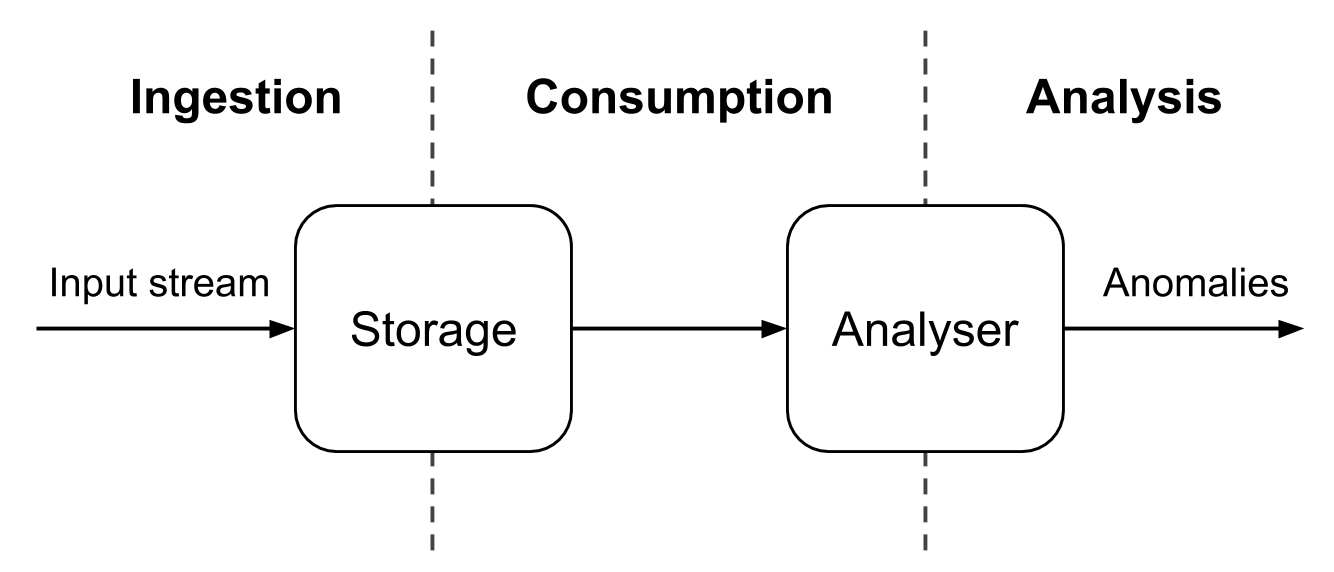
\includegraphics[width=.7\textwidth]{img/eval-arch-1}.
    \caption{General architecture of our solution}
    \label{fig:arch_abs}
\end{figure}

being a specialization of \river{} reference architecture, our data analysis task can be decomposed into three main phases (see Figure \ref{fig:arch_abs}):
\begin{itemize}
\item data ingestion -- data is collected from the mobile network and transferred to a storage layer.
\item data consumption -- data is transferred from the storage layer to the analysis layer.
\item data analysis -- data is processed and results are generated by joining streaming data with the static models.
\end{itemize}

Note that we add a storage layer between ingestion and consumption to decouple the two phases. This means that we can ingest data in real-time, and analyze it at a later stage. This also enables various operational scenarios.
%%
%\paragraph{Infrastructure}
An infrastructural choice specifies where a solution is deployed. The hardware used to run an application can be bought, or rented from a cloud service provider. We restrict our analysis to cloud services, since they usually reduce the operational cost of the solution.

When instantiating virtual machines (VMs), cloud service providers usually offer two types of billing policies: pay-per-use instances and reserved instances. Reserved instances (RIs) can be held for a fixed amount of time at a reduced price with respect to pay-per-use instances. RIs are well-fit to reduce the cost of continuous data analysis solutions, while pay-per-user instances are better fit for bursty workloads, such as periodic analysis tasks. In the following, we refer to pay-per-use instances as shared.

\begin{table}[ht]
  \centering
    \caption{Azure VM sizes (January 2018)}
  \begin{tabular}{@{}lrrr@{}} \toprule
  VM Type & Cores & RAM (GB) & S/R (\euro/month)\\
    \midrule
  VM1 & 2 & 4 & 64.62/60.33\\
  VM2 & 4 & 8 & 127.99/121.58\\
  VM3 & 8 & 16 & 256.61/242.42\\
  VM4 & 16 & 32 & 513.23/484.92\\
    \bottomrule
  \end{tabular}
    \label{tab:sizes}
\end{table}

Table \ref{tab:sizes} presents the characteristics of the virtual machines used in this study. The last column contains the approximated cost of running a shared instance versus a reserved instance. 
The reported costs and characteristics refer to Fsv2-series VMs of Microsoft Azure\footnote{https://docs.microsoft.com/en-us/azure/virtual-machines/windows/sizes-compute}. We chose the Fsv2-series because it is equipped with computation optimized hardware that fitted our needs at affordable cost.
Nevertheless, reported costs do not differ significantly from those of other cloud service providers. 

%\paragraph{Architecture}
%We designed our solutions according to the general architecture depicted in Figure~\ref{fig:arch_abs}. 
%
%The storage layer is responsible for ingesting data in real-time from the mobile network. Due to the arbitrary velocity of the mobile data stream, the streaming storage must be able to scale seamlessly to huge data volumes. Moreover, the streaming storage must be able to record data continuously, since this is one of our operational requirements. The space required to store the generated models is constant, and it can fit comfortably into memory. The storage cost for the raw CDR data is not considered in our analysis, since in the real use case we can aggregate data on-line using windowing operators.
%
%The analysis layer is responsible for processing data and producing results. The analysis layer communicates with the storage layer to retrieve the data, and it produces the results by performing the necessary aggregation queries. Data processing can happen continuously or periodically. We consider both settings in our analysis.
%
%Note that our architecture is related to the lambda architecture (see Section~\ref{sec:vel-arch}), since we produce results by combining data from both batch and speed layers.

%\subsubsection{Implementation Details}

\begin{figure}[ht]
  \subfloat[]{
      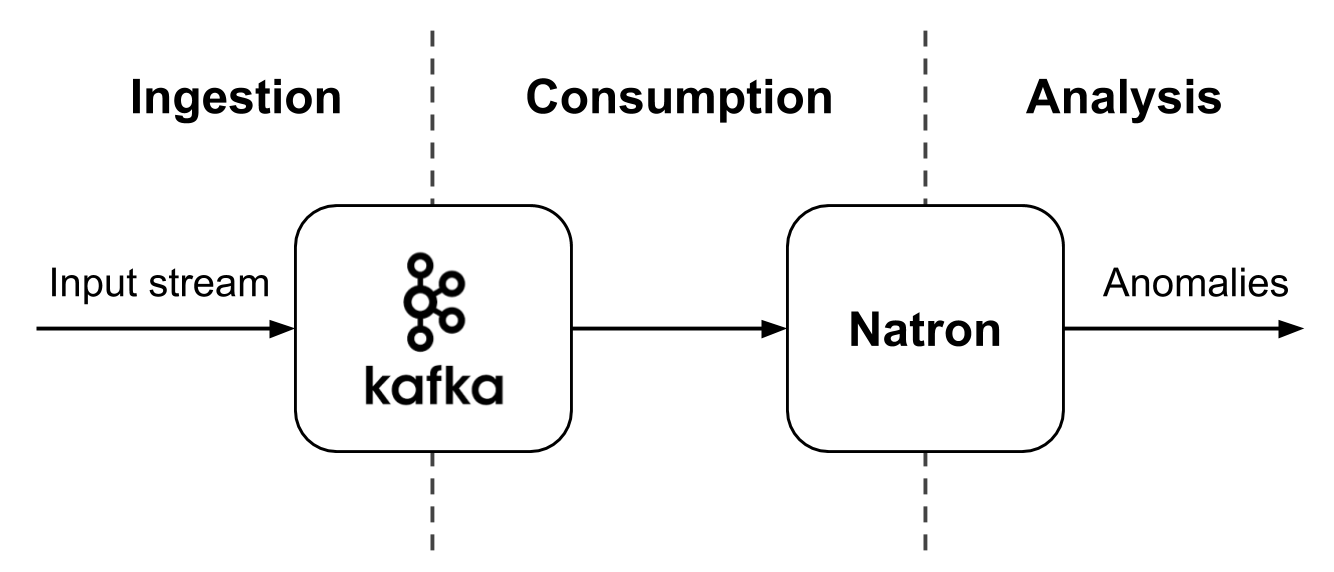
\includegraphics[width=.49\textwidth]{img/eval-arch-2}.
    }
    \subfloat[]{
      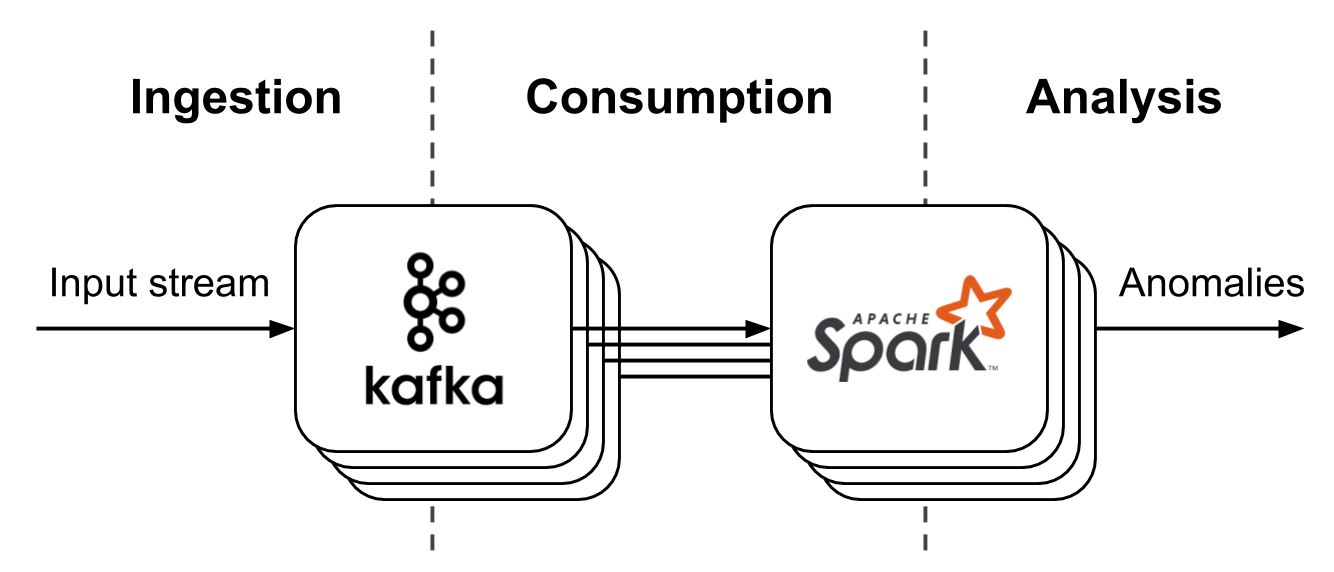
\includegraphics[width=.49\textwidth]{img/eval-arch-3}.
    }
\caption{(a) Architecture for the single-threaded solution. (b) Architecture for the distributed solution}
\label{fig:arch_impl}
\end{figure}

In this work, we use Kafka (see Section~\ref{sec:kafka}) as our streaming data storage. We use two different configurations, one for each solution. The single-threaded solution, based on \sti{}, reads data from a single VM1 machine. The distributed solution, based on \sparkdi{}, reads data from a Kafka cluster composed of four VM2. In the distributed setting, we set the number of partitions for each topic to eight. We choose this value by considering the number of executors used in the experiments, since executors can read in parallel from different partitions.

In the single-threaded solution, the consumption phase is implemented using a Kafka Ingester that polls the data from the server in comma separated value format. The architecture for this solution is depicted in Figure \ref{fig:arch_impl}(a). The Ingester connects to an Apache Kafka server that provides the data. The data enters the system as a stream of generic objects. Each object contains its event timestamp. Downstream to the Ingester, a Processor takes the data from the Bus and transforms each element into a domain-specific Java object (i.e. a Java representation of a CDR, named PixelCDR).

Then, an Processor based on Esper (see Section~\ref{sec:esper-epl}) performs the analysis. The internal stream of PixelCDRs flows into Esper, which performs the query presented in Listing~\ref{lst:epl_query}. The query counts, every 15 minutes, the number of calls/SMSs grouped by pixelId, i.e. the pixel identifier.
The window operation is performed on the event timestamp. We use Kafka exactly-once message delivery to analyze the whole data stream. The query produces the list of anomalous pixels.
The anomalies are identified using the \textit{isAnomalous} user defined function, that access the models file, stored in memory, and implements Equation~\eqref{eq:zscore}.
The query results are then saved to the file system by an Emitter.

\begin{figure}[ht]
\begin{minipage}{0.95\linewidth}
\begin{lstlisting}[caption={EPL query performed by Esper Processor.},frame=single,captionpos=b,label=lst:epl_query,style=ESPER]
SELECT pixelId, MAX(timestamp)
FROM PixelCDR.WIN:EXT_TIMED_BATCH(timestamp, 15 min) 
GROUP BY pixelId 
HAVING isAnomalous(pixelId, COUNT(*), MAX(timestamp))
\end{lstlisting}
\end{minipage}
\end{figure}

We implemented our distributed streaming pipeline using \sparkdi{} and we register both the static models table, and the CDR data stream as temporary views that can be queried through the Structured Streaming API. The CDR view is actually a dynamic table that gets updated as data is ingested. The anomaly detection method is implemented as a SQL query that performs a join on the aforementioned tables, and filters the results based on the anomaly condition defined in Equation \eqref{eq:zscore}. Listing \ref{lst:sql_query} contains the pseudocode for the query.

\begin{figure}[ht]
\begin{minipage}{0.95\linewidth}
\begin{lstlisting}[caption={Spark SQL anomaly detection query.},frame=single,captionpos=b,label=lst:sql_query,style=SPARKSQL]
SELECT pixelId, timestamp
FROM (
	SELECT cdrs.pixelId, cdrs.timestamp, COUNT(1)
	FROM cdr_stream AS cdrs
	WINDOW ON cdrs.timestamp EVERY 15 minutes
	GROUP BY cdrs.pixelId
) AS windowed_cdrs LEFT JOIN models 
ON models.timestamp = windowed_cdrs.window.start 
WHERE isAnomalous(windowed_cdrs.value, model.mean, model.sd)
\end{lstlisting}
\end{minipage}
\end{figure}

The distributed application is deployed on a multi-node Spark cluster, while data is ingested from a multi-node Kafka cluster. This deployment is represented in Figure \ref{fig:arch_impl}(b). Spark is integrated with Kafka to provide parallel reads from multiple Kafka partitions. 

We choose Apache Spark for our distributed solution due to its wide spread use in industry, and the availability of previously developed source code and expertise.
%%
%\subsubsection{Operational considerations}
Operational requirements are related to business choices (see Section~\ref{sec:uda-analysis}). They deal, for example, with how often a result report should be produced. We consider the following two operational scenarios:
\begin{itemize}
\item \textit{Continuous ingestion -- continuous consumption and analysis}. This scenario includes real-time use cases, such as crowd monitoring for security purposes. Data is consumed as soon as it is produced, and the delay with which results are produced corresponds to the latency of the system. In this regime, results are produced continuously with whatever latency the system might have. This scenario requires the continuous utilization of reserved resources, since the solution must run without interruptions.
\item \textit{Continuous ingestion -- periodic consumption and analysis}. Periodic analysis represents a common scenario. In many use cases, the results of the analysis can be summarized in a periodic report, and the real-time analysis is not necessary. The ingestion layer must still run continuously to avoid data losses. On the other hand, the analysis layer can be allocated only for the amount of time needed to perform the analysis and generate the results.
\end{itemize}

Another important considerations when designing an industrial analytics system are fault-tolerance and redundancy. Apache Kafka and Apache Spark respectively provide out-of-the-box redundancy and fault-tolerance. Nonetheless, we do not include these aspects in our analysis, since the total solution cost of a fault-tolerant system can be approximated as the total solution cost multiplied by the redundancy factor. If we apply this consideration to both solutions, it does not affect our final results.

\subsection{Experimental Settings}
The goal of our experimental methodology is to find the most cost-effective solution for the given problem. To assess this, we run our solutions on both real and simulated problem instances. The real data MOB1 is collected from the mobile phone network of TIM. Starting from this real data we generated several other datasets (MOB10, MOB30, etc.). Those datasets were generated to analyze the scalability of our solutions. 

We compare our solutions based on their total cost when they both provide correct results. This is not always the case since the most economic single-threaded configurations struggle to deal with the most demanding problem instances. The solution cost is computed by multiplying the cost of the solution (i.e., price-per-second of the used VMs) with the execution time of the experiment (if completed correctly). The cost of the solution also depends on the operational requirements, e.g., a continuous solution can run on reserved instances, thus reducing the price-per-second.

We executed all experiments on Microsoft Azure Linux VMs. For each experiment, we performed five experimental runs. All reported results are average over four runs by discarding the worst outcome. We do not include error bars in the plots since their bounds are so tight that they simply overlap with the point shapes and clutter the images.

We do not consider latency in our analysis due to the following reasons:
\begin{enumerate}
\item In the continuous analysis scenario, at regime the latency of the system does not influence the stream of results. Moreover, the latency to analyze one minute of data is below 1.5 seconds for both solutions, which is appropriate for our use case.
\item In the periodic analysis scenario, the latency of both systems is negligible with respect to the periods considered (i.e. every day or every week).
\end{enumerate}
Thus, in the following we omit latency from our discussion.

%\subsubsection{Configurations}
Our goal is to find the most cost-effective configuration which solves the problem. We restrict our analysis to Fsv2-series VMs under the assumption that in cost-aware scenarios more general-purpose VMs are preferable to workload-optimized VMs, since they can be shared and used by different workloads. Figures \ref{fig:tuning}(a) and \ref{fig:tuning}(b) show the solution cost as a function of the scale factor for different configurations of \sti{} and \sparkdi{}. 

%\paragraph{\sti{} deployment}
\sti{} was deployed using a docker container to create a sandbox environment and to ease the monitoring operations for CPU and memory consumption. The whole infrastructure needed a single VM for each experiment in addition to the VM needed for the data provider,  i.e. a single partition Kafka server on a VM1.
We run multiple experiments for each dataset and remove the outliers, e.g. the first run of each experiments was considered as a system setup, collect data result for correctness check, i.e. anomalies, and CPU/memory consumption log to monitor the health of the infrastructure. During each run the container exploits all available virtual machine resources for the computation. We vary the dimension of the VMs in azure to stress the environment and get the upper limit of the resource needed to handle a given amount of data.

We experimented with three configurations, having different number of cores, RAM, disk I/O, and network I/O available: (i) \sti{}1 with a single VM1, (ii) \sti{}2 with a single VM2, and (iii) \sti{}3 with one VM4.

The single-threaded implementation suffers from the volume of the data, a single VM cannot scale horizontally to deal with a continuously increasing amount of data. 
Figure~\ref{fig:tuning}(a) clearly shows that the different configurations can bear different loads of data.
\sti{}1 can handle dataset MOB1, which represents the original data size, and can perform the anomaly detection in about 120 seconds. This configuration can handle up to dataset MOB10, but bigger dataset results are problematic. Configurations \sti{}2 and \sti{}3 can bear at most dataset MOB50 and MOB100  (respectively), but are more expensive than configuration \sti{}1 .
The three chosen configurations widely explore the hardware offerings in order to find the best solution related to the data loads. Due to the variability of configurations' behaviors, we tested the system against more dataset than the ones listed in Section~\ref{sec:desc}, i.e. we tested dataset with scale factor k=2, k=3, k=5, and k=20.

We compare all the three \sti{} configurations with the best configuration chosen for the distributed system in order to have a complete overview for the different input volumes. During the experiments, regardless of the \sti{} configuration, the normality models are loaded in memory, while streaming data is read from the Kafka cluster described in Section \ref{sec:kafka}.

%%
%\subsubsection{\sparkdi{} deployment}
We deployed \sparkdi{} application on a Spark cluster tuned using the total solution cost as a metric, and experimenting with three parameters which commonly affect Spark's performance. Our intention here is to present our findings on the best Spark configuration for our specific use case, datasets, and problem setting. We implemented our Apache Spark cluster using Azure Linux VMs (see Table \ref{tab:sizes}).

\begin{figure}[t!]
  \subfloat[]{
    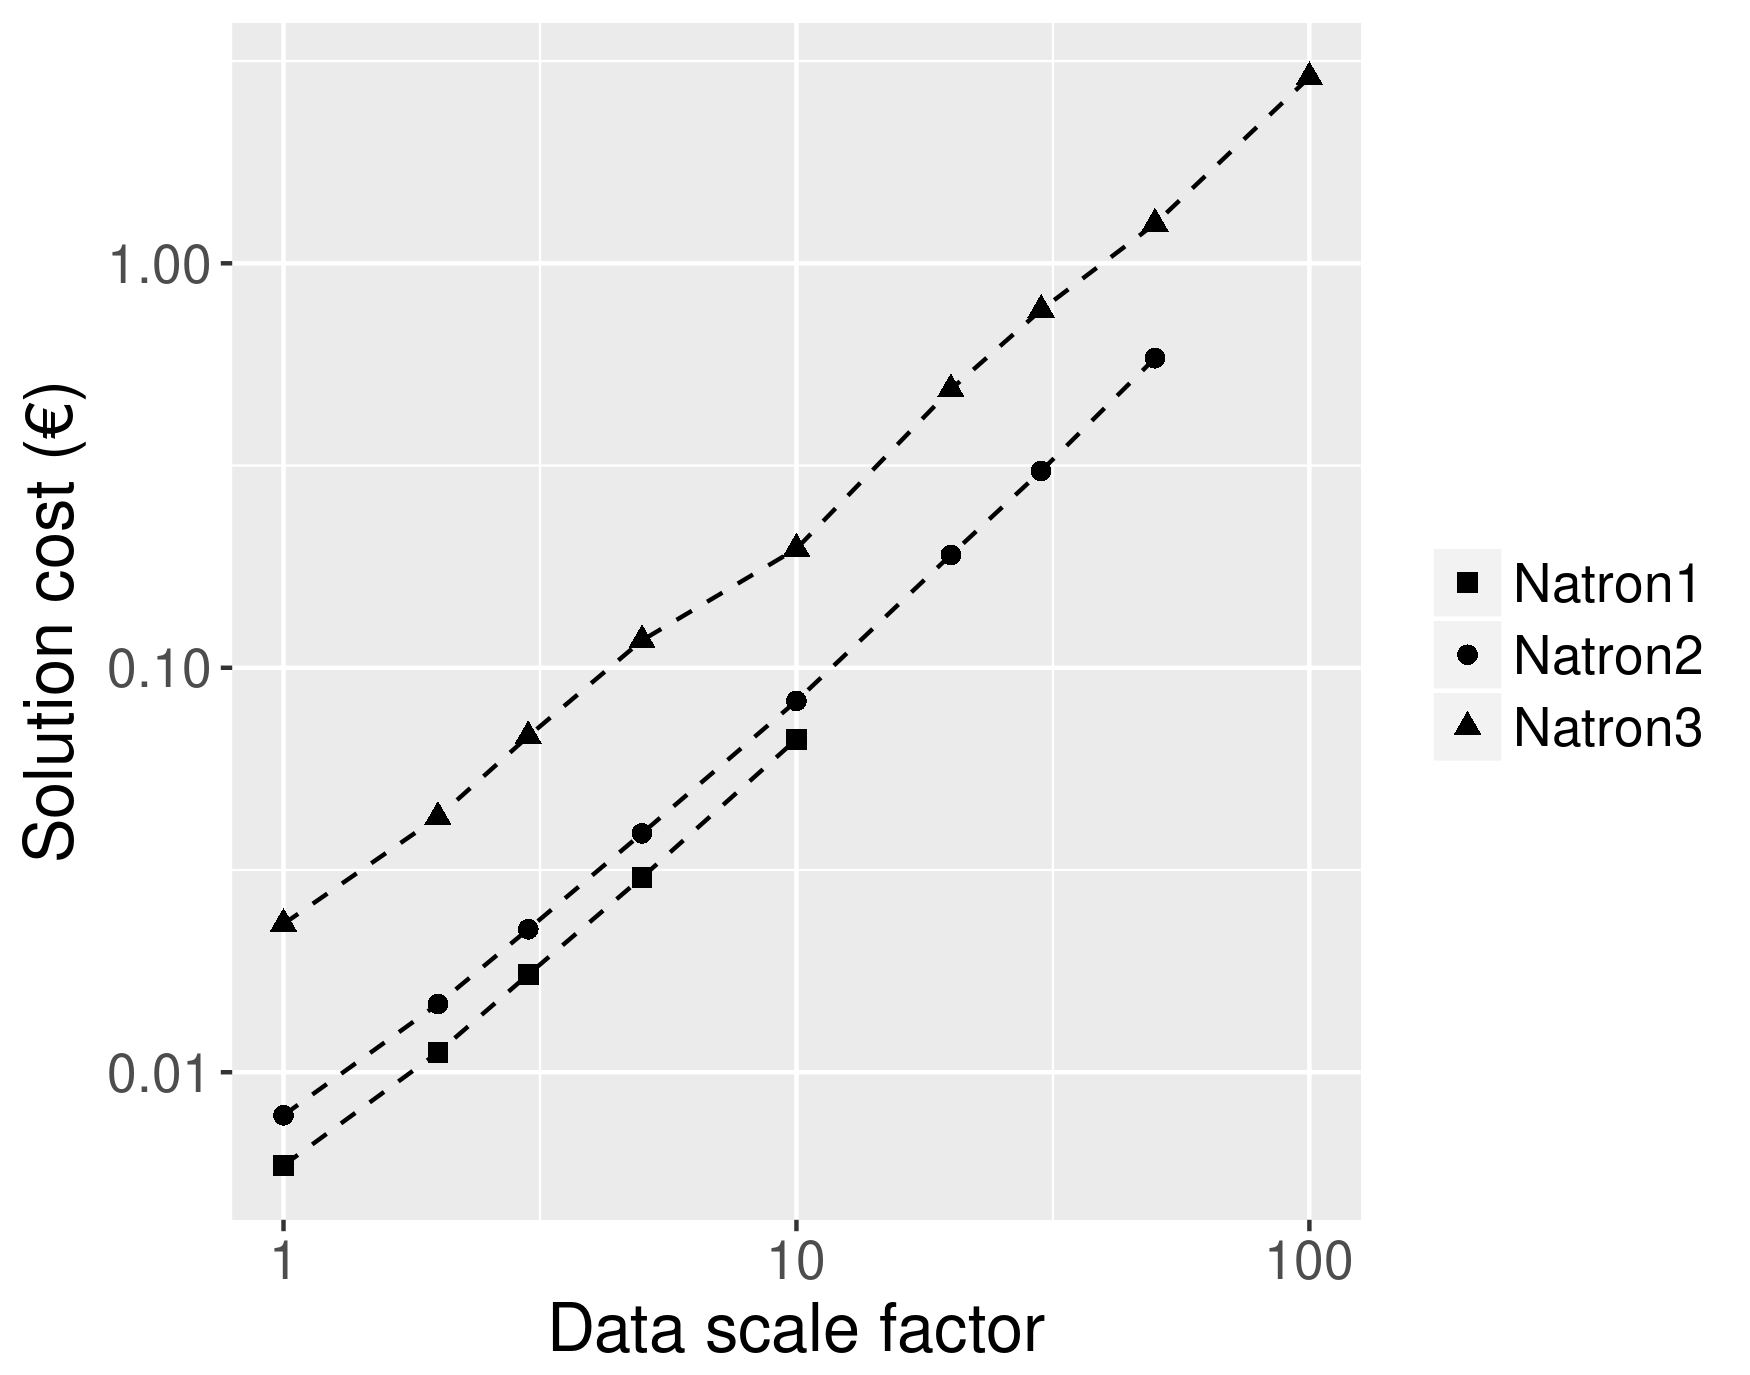
\includegraphics[width=.49\textwidth]{img/eval-natron_base}.
  }
  \subfloat[]{
    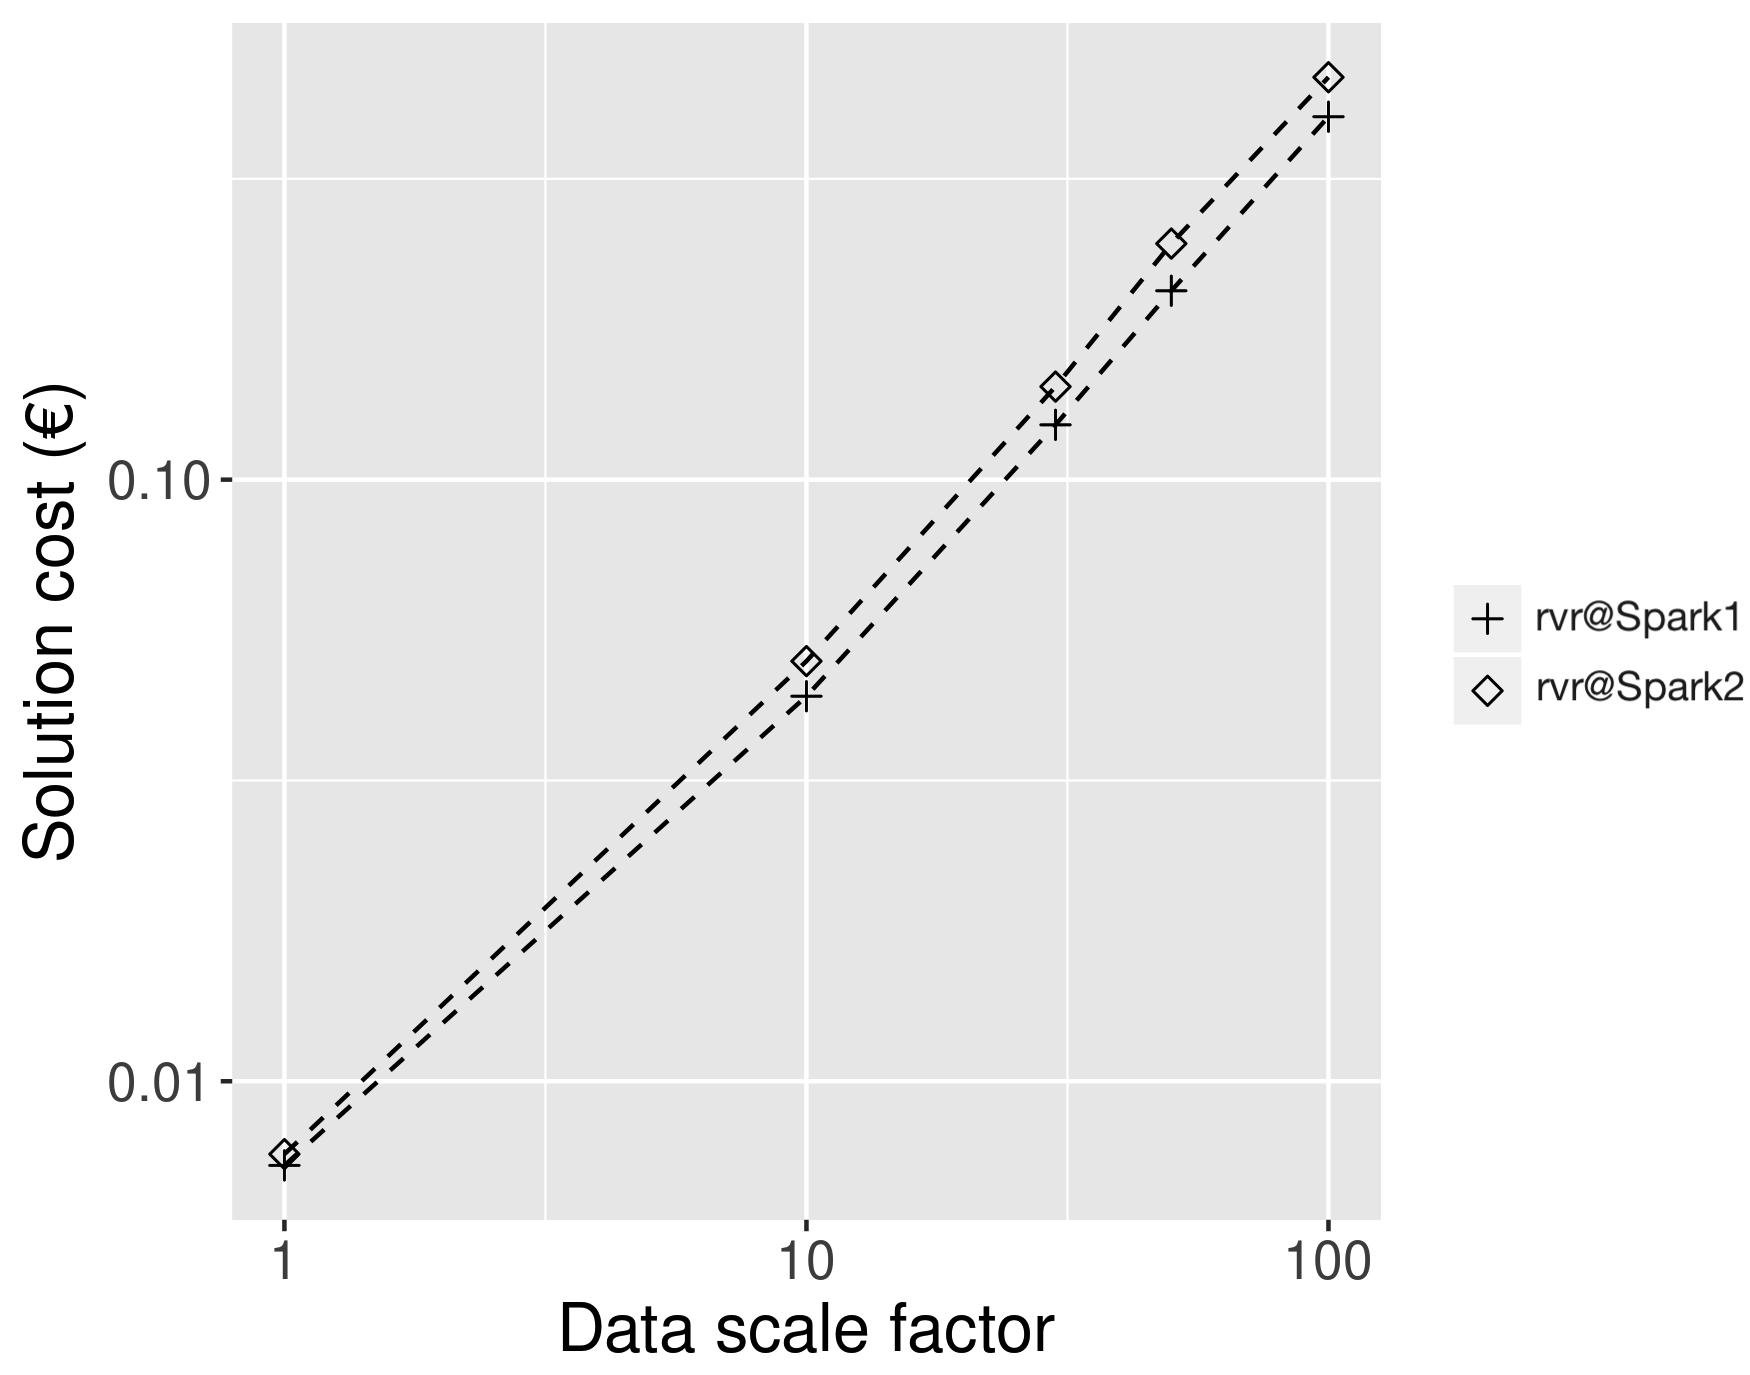
\includegraphics[width=.49\textwidth]{img/eval-spark_time_vs_size}.
  } \\
  \subfloat[]{
    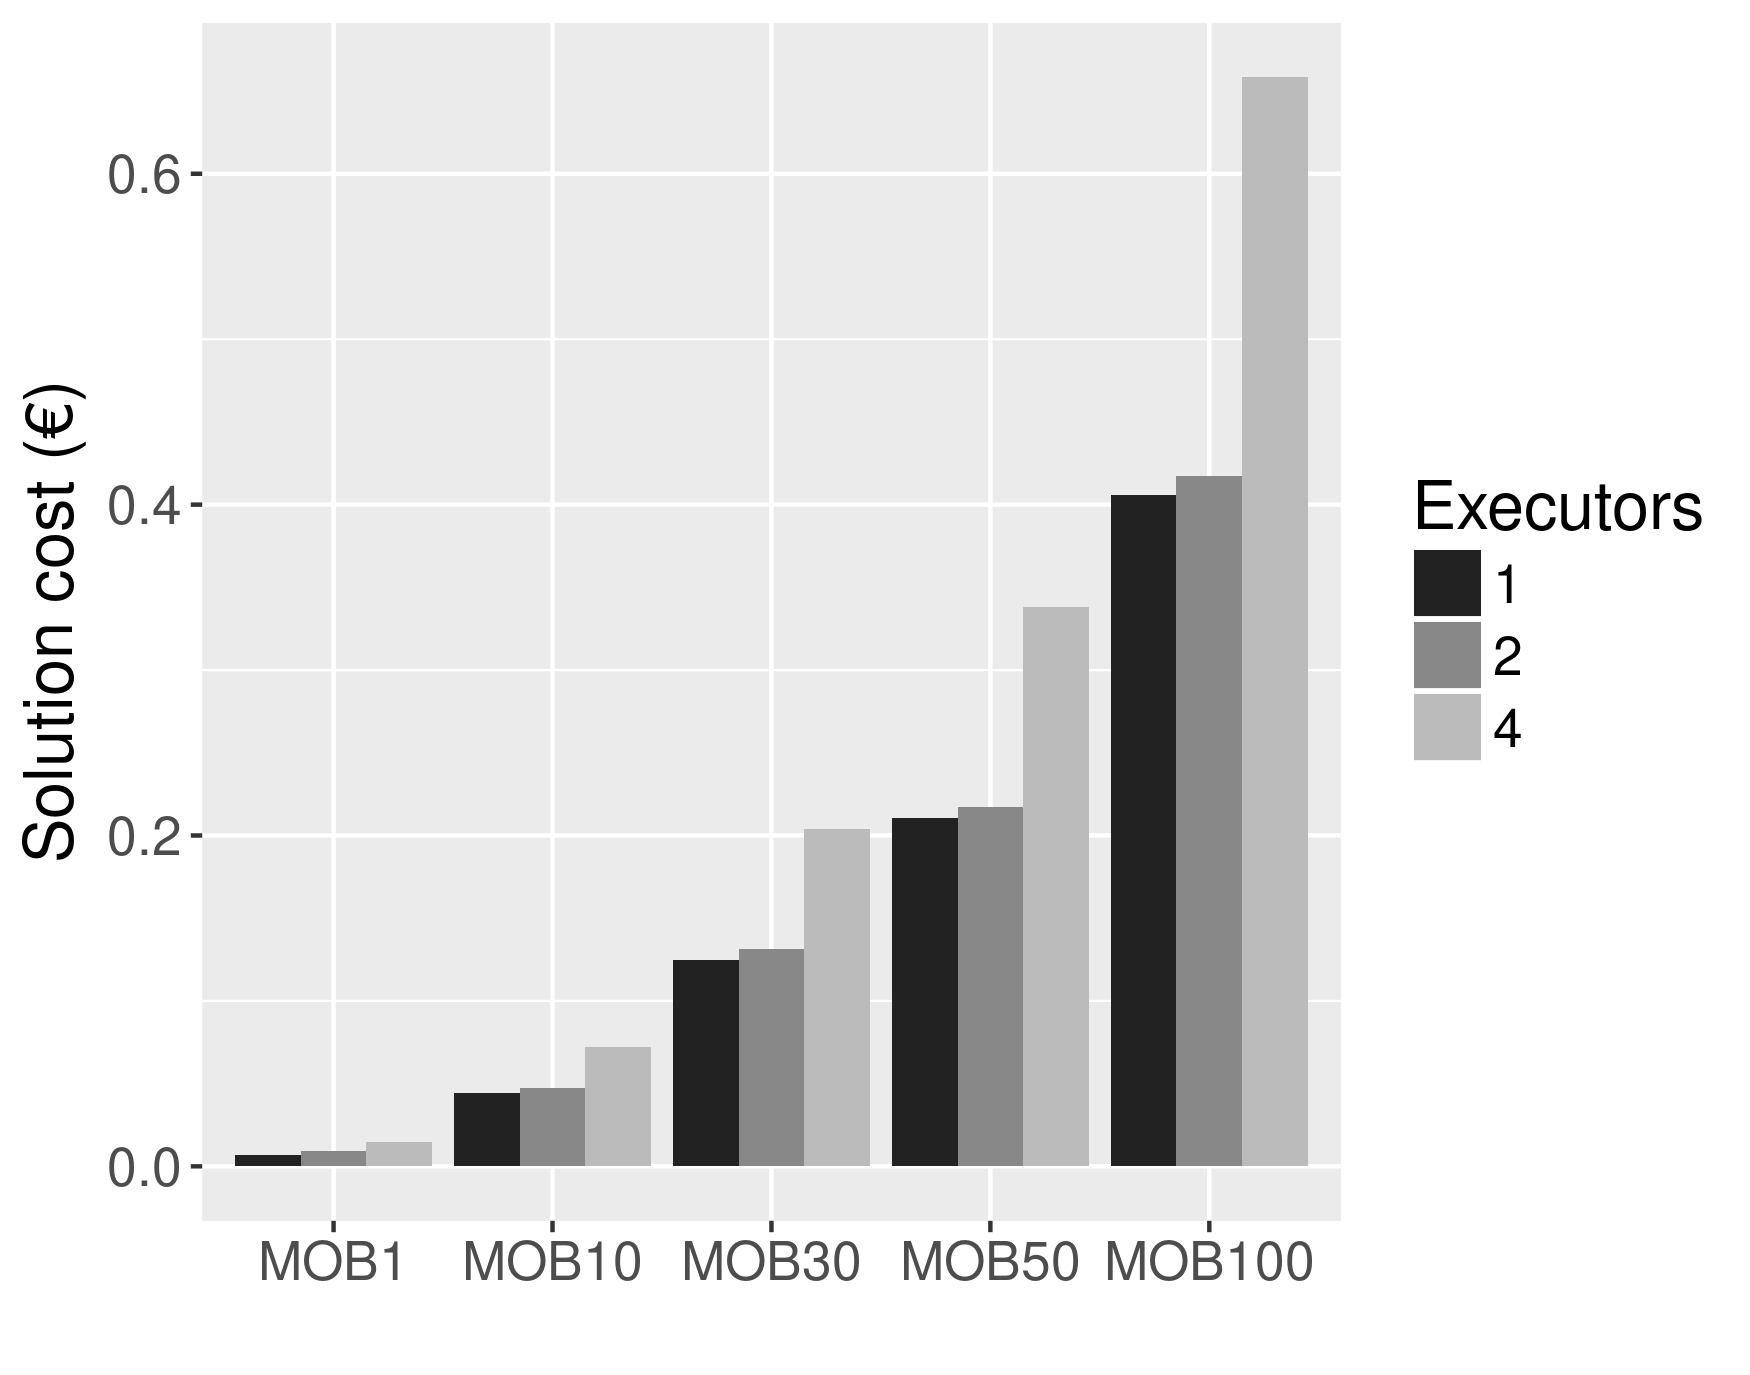
\includegraphics[width=.49\textwidth]{img/eval-spark_time_vs_executors}.
  }
  \subfloat[]{
    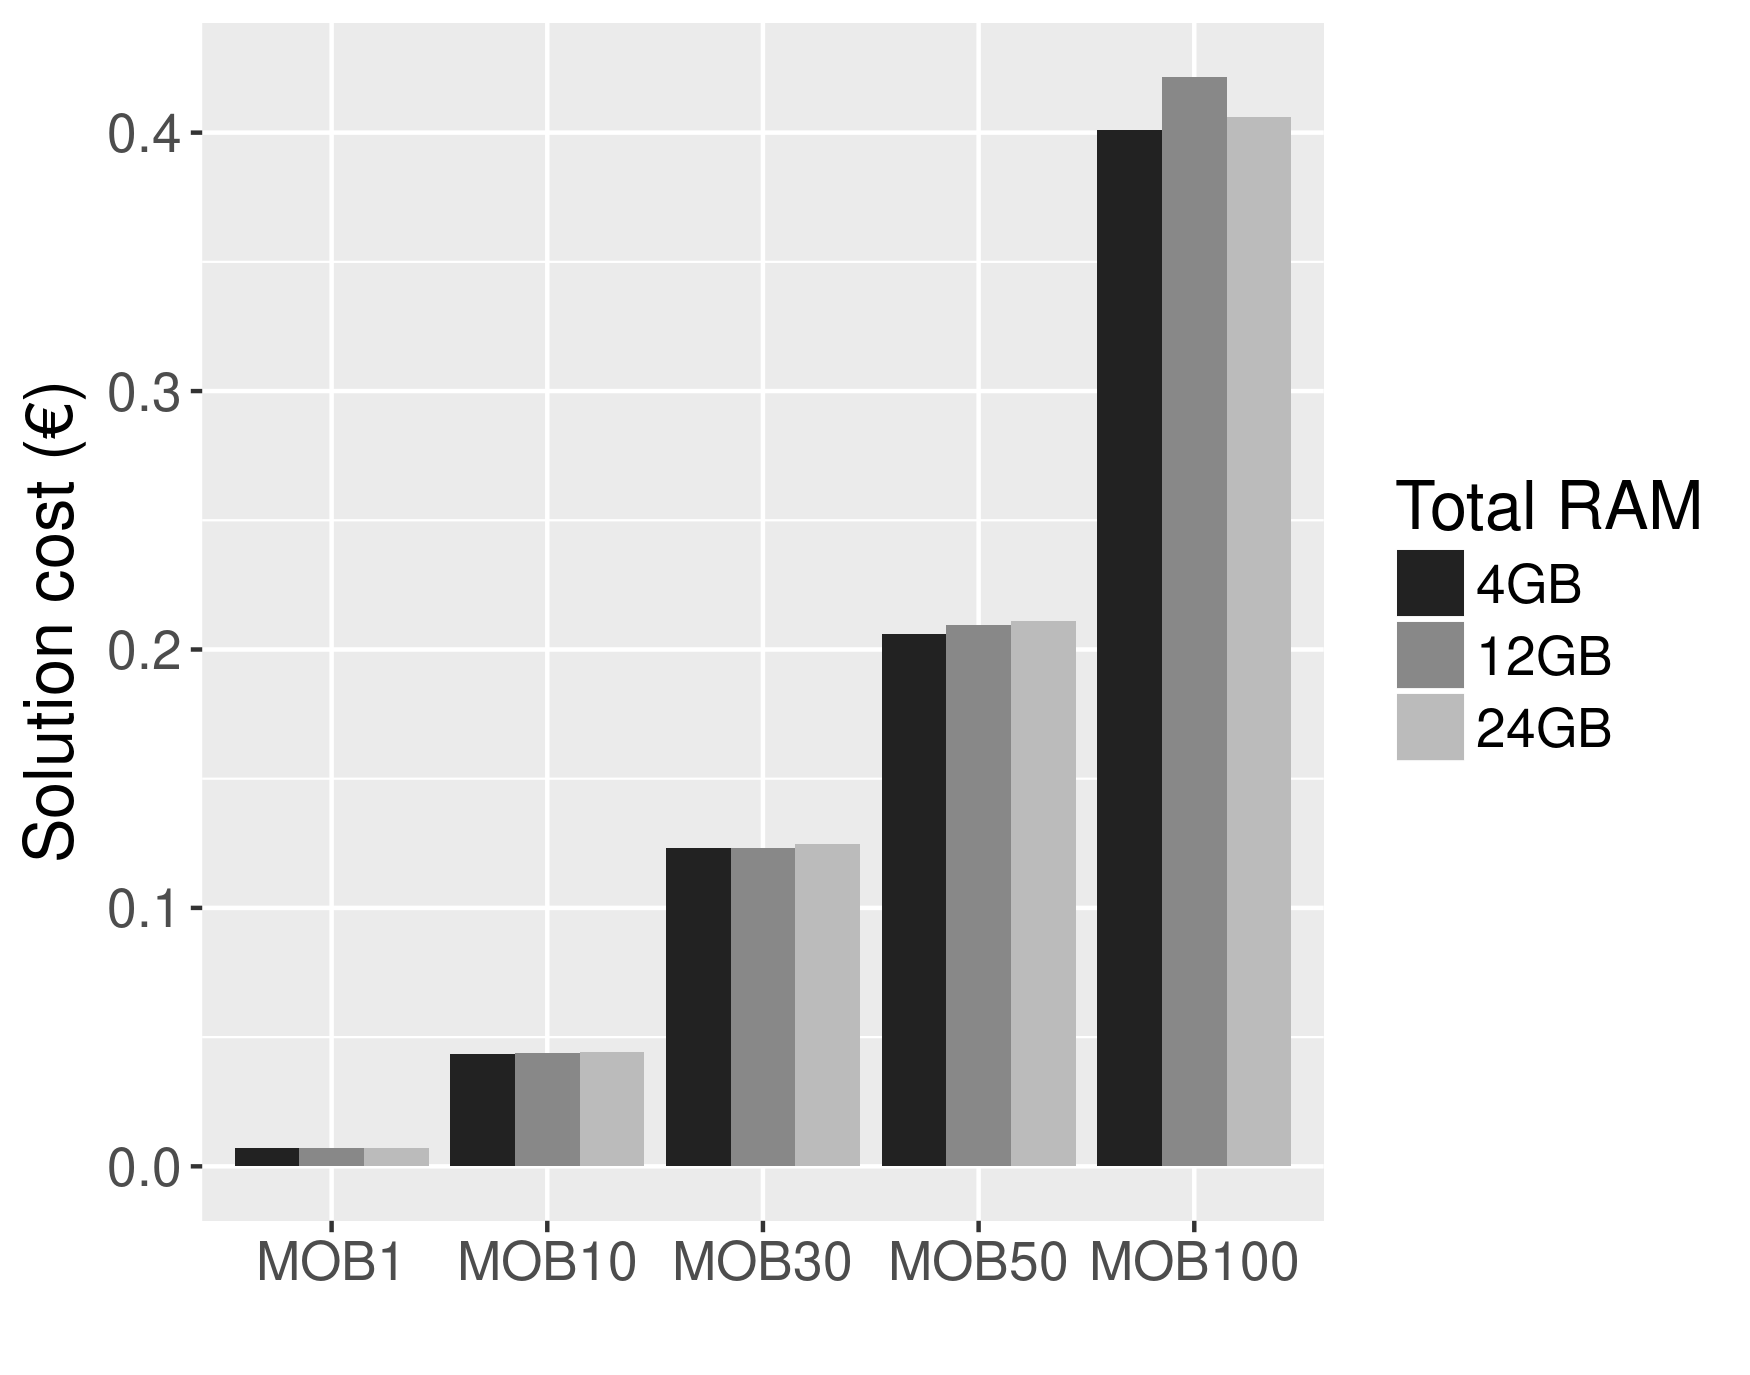
\includegraphics[width=.49\textwidth]{img/eval-spark_time_vs_ram}.
  }
\caption{(a) Solution cost over data scale for different \sti{} configurations. (b) Solution cost over data scale for different \sparkdi{} configurations. (c) Solution cost over number of executors per worker on different datasets (RAM at 24GB). (d) Solution cost over total number of RAM in GB for different datasets (1 executor per worker).}
\label{fig:tuning}
\end{figure}

We experimented with the following cluster parameters: i)the virtual machine size, ii) the number of executors per worker (or number of cores per executor), and iii) the memory allocated per executor.
All other parameters were set to their default values. Note that, since in Microsoft Azure each virtual core (vCPU) corresponds to a single thread, in the following we use the terms core and thread interchangeably.
%%

%\subsubsection{Virtual machine size} 
Cloud service providers offer several VM types. Those types vary depending on the number of cores, RAM, disk I/O, and network I/O available to user applications running on the VM. Thus, an important consideration when deploying a cloud solution is the choice of VM type.

We evaluated two different cost-equivalent configurations for our Spark cluster (refer to Table \ref{tab:sizes} for VM characteristics): (i) \sparkdi{}1 with one VM2 as a master and four VM2 workers, and (ii) \sparkdi{}2 with a singly VM2 as a master and two VM3 workers.

Note that we also experimented with smaller cluster configurations (e.g., a single VM2 worker). However, we found that these were not as cost-effective as the configurations described above. This might seem counterintuitive. However, consider that a smaller configuration usually takes more time to perform the analysis. Since our metric is the total solution cost, to be cost-effective a solution's cost reduction should compensate for its performance penalty.

As an example, we found out that a cluster with a single VM2 worker takes from 2.75 to 3 more time (depending on the dataset) to perform the task with respect to our \sparkdi{}1 configuration, while only costing 2.5 less.

Figure \ref{fig:tuning}(b) shows the cost of the solution for both configurations. All Spark settings were set to their default values (all available cores, 1GB of RAM per executor). The figure highlights that the \sparkdi{}1 configuration tend to be more cost-efficient, even though the total number of used cores is the same in both configurations.

Even after tuning both clusters, i.e. by changing the default parameters, we could not find a configuration for \sparkdi{}2 outperforming \sparkdi{}1. We used \sparkdi{}1 for all other experiments. The two following sections provide more details on the experiments we performed measuring the sensitivity of the selected configuration to changes in the number of cores per executor and in the amount of RAM per executor.

%\subsubsection{Cores per executor} 
An important parameter in Spark configuration is the number of cores allocated to each executor. The default configuration allocates all available cores. Incidentally, the number of cores per executor also determines the number of executor processes that a worker can spawn. Thus, we perform our sensitivity analysis in term of executors per worker. We fixed the total RAM to 24GB and varied the number of executors per worker machine. Figure \ref{fig:tuning}(c) shows our results. We can see that having a single executor on each worker outperforms other configurations. This is supposedly due to the fact that when multiple executors reside on the same machine, the JVM must handle a large volume of I/O network traffic in order for them to communicate. This could possibly influence application performance.

%\subsubsection{RAM per executor} 
Another important parameter is the amount of RAM designated to each executor. In this case, we picked the best configuration from the previous analysis, i.e. one executor per worker, and varied the RAM allocated to each executor. Figure \ref{fig:tuning}(d) shows our results to this sensitivity analysis. We can notice that the amount of memory allocated to each executor does not seem to affect execution time. This is surprising, considering the common knowledge that Spark performance is proportional to the amount of main memory available. However, our particular use case, i.e. windowed and watermarked relational query, is executed considering one window of data at a time. Even at maximum scale (x100), our windows do not exceed 1GB of RAM, and therefore in this particular scenario the system is not memory-bounded.

All the following experiments were executed using configuration \sparkdi{}1 with 4 cores and 3GB of RAM per executor. The normality models are stored in a static file over the Spark cluster, while streaming data is read from the Kafka cluster described in Section~\ref{sec:kafka}.

\subsection{Results and Discussion} \label{sec:results}

\begin{table}[ht]
\centering
\caption{Operational scenarios. Each layer of the system can run continuously (C) or periodically (P), and on shared (S) or reserved (R) hardware. Data ingestion and consumption are both handled by Apache Kafka, therefore they are always executed on the same hardware.}
\begin{tabular}{@{}lrrr@{}} \toprule
Scenario & Ingestion & Consumption & Analysis \\
\midrule
S1 & C/R & C/R & C/R \\
S2 & C/R & P/R & P/S \\
\bottomrule
\end{tabular}
\label{tab:scenarios}
\end{table}

In this section, we present our experimental results. We organize our discussion based on the operational requirements considered in Section \ref{sec:solutions}. The analyzed scenarios are summarized in Table \ref{tab:scenarios}. 

\begin{table}[ht]
\centering
\caption{Monthly solution costs. The monthly cost of our solution depending on the operational scenario. Notice that if we perform continuous ingestion, the consumption costs are included (Incl.). The third scenario represents the case in which ingestion costs are fixed, i.e. they do not depend on the number of machines, but only on data throughput. The most cost-effective solution is highlighted.}
\begin{tabular}{@{}llrrrr@{}} \toprule
Scenario & & Ingestion & Consum. & Analysis & Total\\
\midrule
S1 & \sparkdi{}1 & \euro486.32 & Incl. & \euro607.9 & \euro1094.22 \\
   & \sti{}3 & \euro60.33 & Incl. & \euro484.92 & \textbf{\euro545.25}\\
\midrule
S2 & \sparkdi{}1 & \euro486.32 & Incl. & \euro12,41 & \euro498,73\\
   & \sti{}3 & \euro60.33 & Incl. & \euro76.85 & \textbf{\euro137.18}\\
\midrule
S3 & \sparkdi{}1 & Fixed & \euro9.93 & \euro12.41 & \textbf{\euro22.34}\\
   & \sti{}3 & Fixed & \euro9.68 & \euro76.85 & \euro86.53\\
\bottomrule
\end{tabular}
\label{tab:monthly}
\end{table}

The resulting monthly solution costs per scenario are represented in Table \ref{tab:monthly}. All costs refer to the MOB100 dataset. Periodic scenarios (S2 and S3) refer to analysis carried out daily, i.e., 30 times per month.

\begin{figure}[p]
  \centering
  \subfloat[]{
      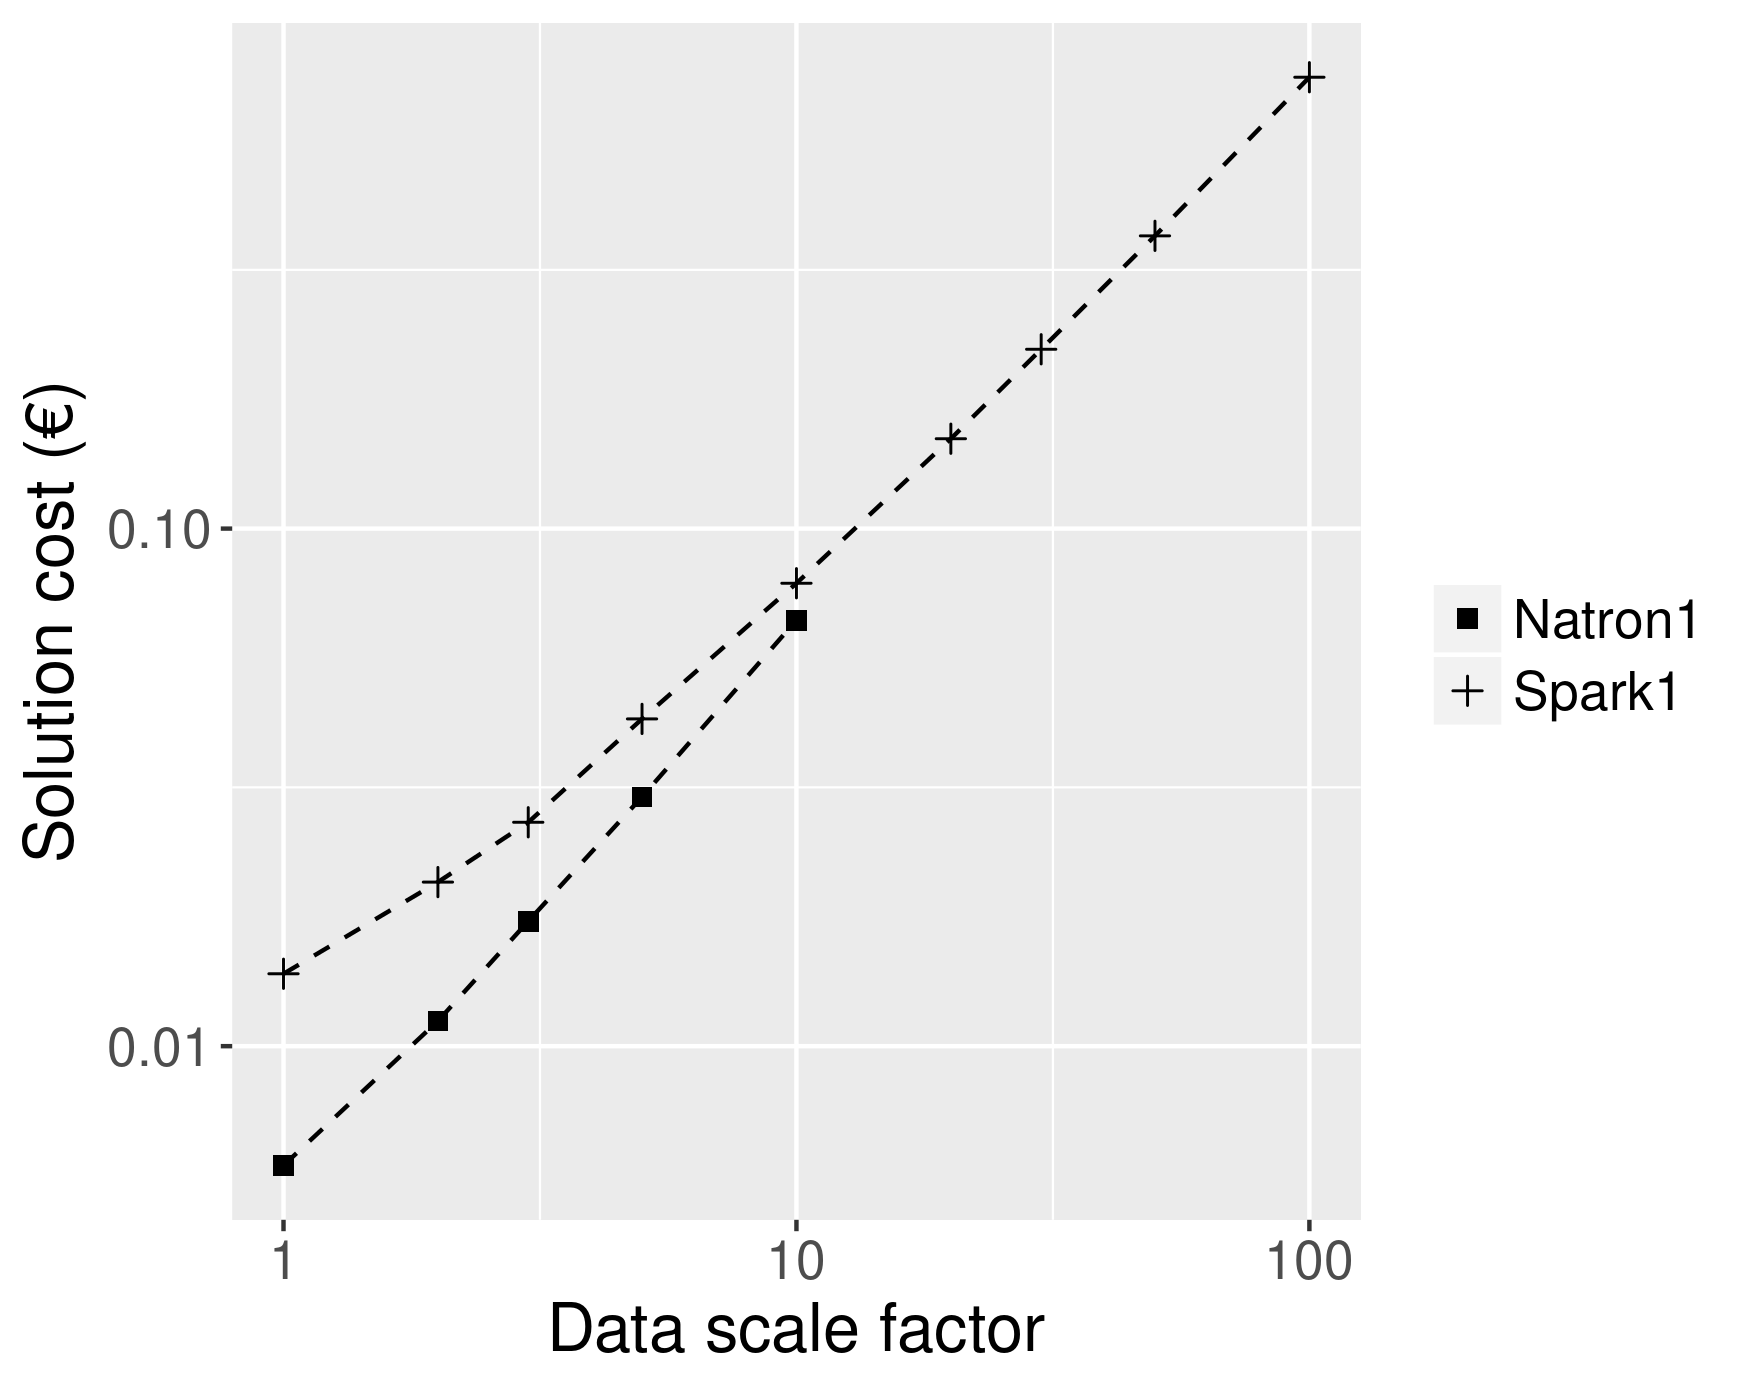
\includegraphics[width=0.47\textwidth]{img/eval-N1_vs_spark}.
    } 
    \subfloat[]{
      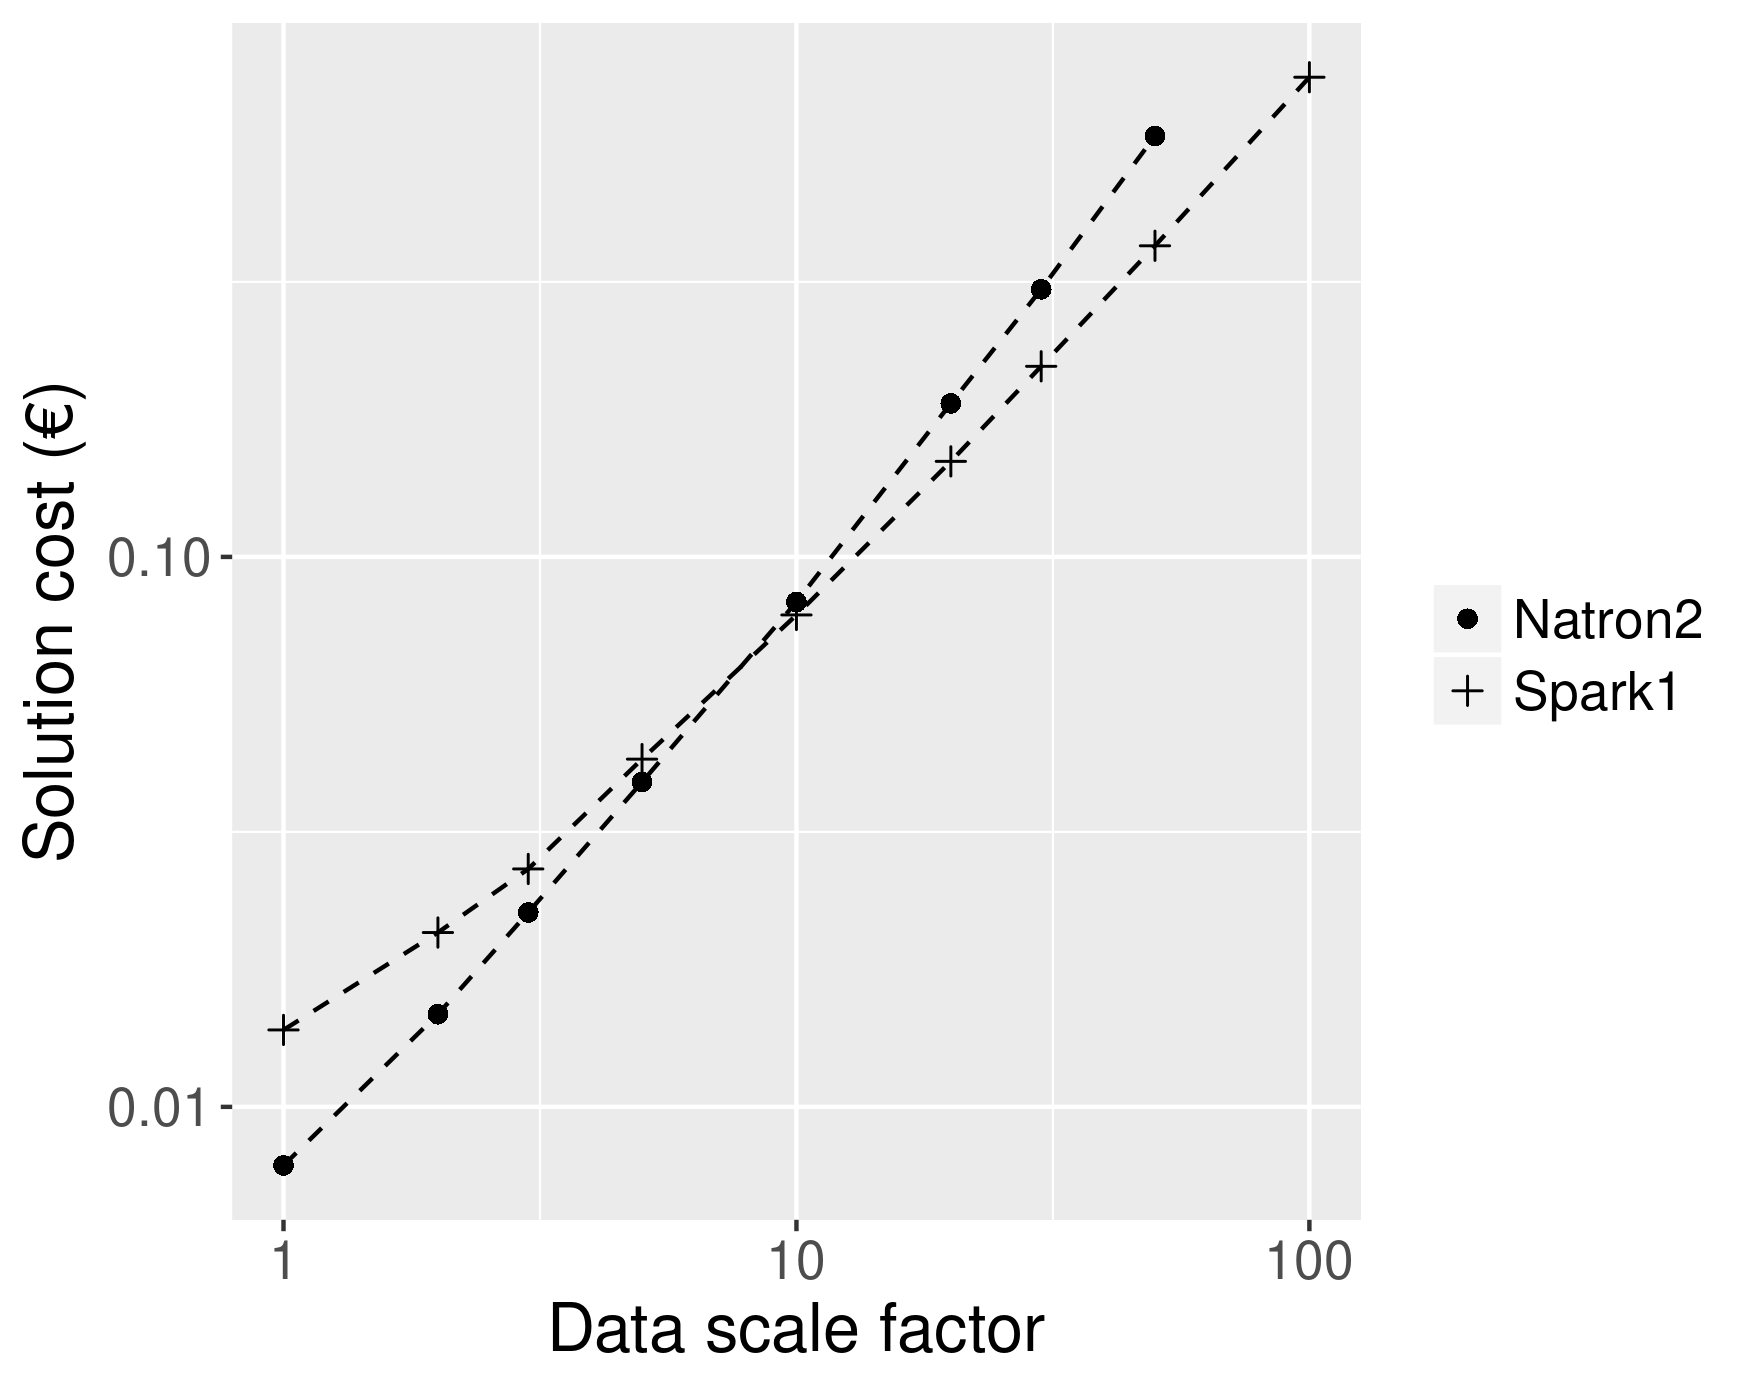
\includegraphics[width=0.47\textwidth]{img/eval-N2_vs_spark}.
    }\\
    \subfloat[]{
      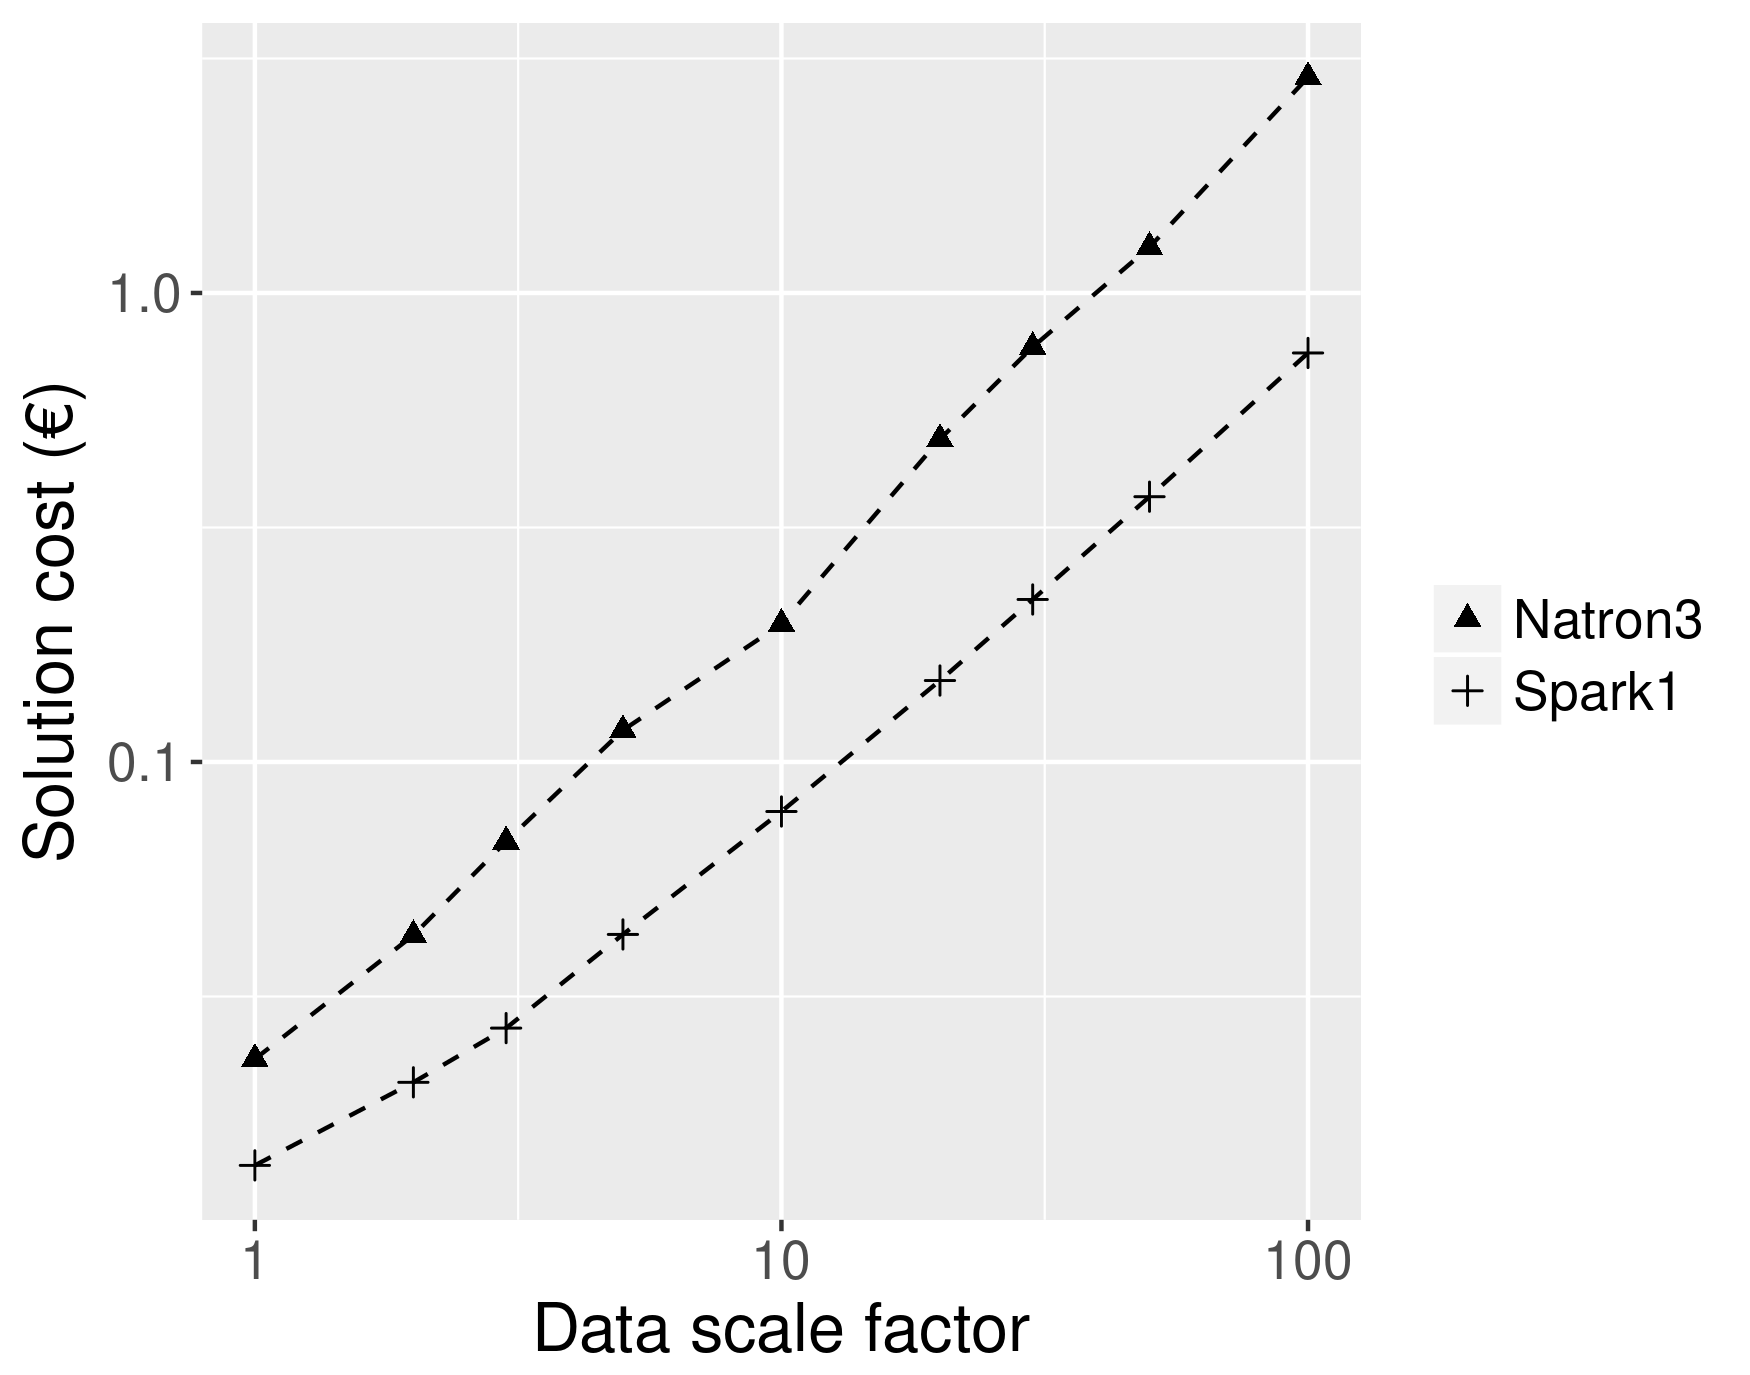
\includegraphics[width=0.47\textwidth]{img/eval-N3_vs_spark}.
    }
\caption{(a) Total solution cost for S3: \sti{}1 vs \sparkdi{}1. \sti{}1 is the lowest cost solution, but it can handle only datasets of modest size. (b) Total solution cost for S3: \sti{}2 vs \sparkdi{}1. The two solutions are cost-equivalent at a scale factor around 10. After that, \sparkdi{}1 becomes the most cost-effective solution. (c) Total solution cost for S3: \sti{}3 vs \sparkdi{}1. \sti{}3 can handle all datasets considered, however it is less cost-effective than the distributed system at all scales.}
\label{fig:NvsSpark}
\end{figure}

\medskip

\textit{S1 -- Continuous ingestion -- continuous consumption and analysis}
In this scenario, we consider the case in which we require a continuous analytics solution. The whole infrastructure must be continuously up and running to support the ingestion, consumption and analysis phases. We can compute a monthly solution cost by considering the reservation price of all VMs used in the solution. 

From Table \ref{tab:monthly}, we can see the estimated monthly solution cost for scenario S1. Ingestion cost is calculated using reserved instance price, since these machines must run continuously. This is the same for analysis cost. Consumption cost is included in the ingestion, since the Kafka VMs perform both phases continuously. The single-thread cost is calculated considering configuration \sti{}3. 

In this case, we can clearly see that the single-threaded implementation is the most cost-effective solution for the problem.

\medskip

\textit{S2 -- Continuous ingestion -- periodic consumption and analysis}
This scenario represents a use case where the continuous analysis is not necessary, but periodic reports are needed. Table \ref{tab:monthly} contains the cost analysis for this scenario. The costs of ingestion and consumption are equivalent to S1. The analysis cost is computed on the more demanding dataset MOB100, using \sparkdi{}1 and \sti{}3 configurations. We report the monthly cost for an analysis performed daily. The ingestion phase must be continuous and, consequently, the infrastructure that support the ingestion and consumption phases can be deployed on reserved hardware. The analysis is periodic (once a day), and can be executed on pay-per-use VMs which can be turned on only for the duration of the analysis. 

In this scenario, we can see that the \sparkdi{} system is more cost-effective with respect to the analysis phase, but not to the ingestion phase. The cost of continuously ingesting data using a distributed cluster outvalues the benefits of processing such data in parallel. This is still true at lower data scales, where the convenience of the single-threaded solution is even more evident.

After realizing this fact we included a final scenario (\textit{S3}) in our analysis. This scenario is a situation where data ingestion is provided at a fixed and small price, i.e. it does not depend on VMs cost but only on data throughput and retention. This is the case with some particular offers from cloud providers such as Confluent\footnote{\url{https://www.confluent.io}}. Since the throughput and the retention are fixed, in this scenario the ingestion cost is the same for both solutions.

\medskip

\textit{S3 -- Continuous ingestion at fixed/small price -- periodic consumption and analysis}
In this scenario the total cost of the solution depends on the number of machines active during the analysis phase, and on the duration of this phase. Thus, if the additional costs of using more machines in the distributed setting implies reducing the execution time by the same factor, then the distributed solution is the most cost-effective.

Table \ref{tab:monthly} presents the results for this scenario. The results  compare configuration \sparkdi{}1 versus configuration \sti{}3 when processing the dataset MOB100. We assume the analysis is carried out periodically each day. We can see that the reduced execution time for the analysis makes up for the increased number of VMs. This makes the distributed solution around 3.8 times more cost-efficient than the single-threaded system.

We provide more insight on this scenario by considering different data scales. We compare configuration \sparkdi{}1 with the less expensive \sti{} configuration that can handle a given data scale: configuration \sti{}1 for a scale factor up to 10, configuration \sti{}2 for a scale factor up to 50, and configuration \sti{}3 for the dataset MOB100.

We can see that, in this setting, the most cost-effective solution depends on the data size. At small data scales, configuration \sti{}1 is the most cost-effective solution. The configuration \sti{}1  can only deal with data volumes up to scale factor 10 (city scale), but, until this point, it is more cost-effective than configuration \sparkdi{}1 (Figure~\ref{fig:NvsSpark}(a)). When the data size increases, the solutions first become equivalent in term of cost around city scale (Figure~\ref{fig:NvsSpark}(b)), and, then, configuration \sparkdi{}1 becomes the most cost-effective solution (Figure~\ref{fig:NvsSpark}(c)) when dealing with national and extreme scales.

The results presented in this section show that in case of continuous analysis, the single-threaded solution is the most cost-effective option.

When periodic analysis is considered, the distributed solution is the most cost-effective in analyzing the data. However, this benefit is outvalued by the costs of distributed data ingestion. Thus, the single-threaded application remains the best choice also in this case.

Finally, if we assume that data ingestion costs only depends on data throughput and retention, i.e. they are fixed and small, we show that the most cost-effective choice depends on the data size. The single-threaded application is cost-effective when managing small datasets, which is our setting are the CDRs generated by Milan when including Internet or those of the entire Italy if limiting the analysis to calls and SMSs. However, as the data size grows to the size of Italy including Internet, the distributed solution becomes the most cost-effective option.

\section{Conclusion}

In this chapter, we investigate how to implement \river{} computational model from different points of view.
We concentrate our effort on the implementation of the \textit{Lazy Transformation} approach.

We present \sti{} (see Section~\ref{sec:comp-mod-impl-v}) -- a single-threaded, vertically scalable implementation of the \river{} computational model -- and we evaluate it against our Streaming Linked Data Framework (SLD) that applies data transformation at ingestion time (see Section~\ref{sec:comp-mod-eval-performace}).
The result of this evaluation validates Hypothesis \textsf{Hp.2.1}: \sti{} results better than SLD under both resource consumption and correctness points of view.

Comforted by the results of this performance evaluation, we assume the \textsf{Lazy Transformation} as a third principle \textbf{(P3)} of our computational model and we apply it in the horizontally scalable implementations based on distributed technologies (see Section~\ref{sec:comp-mod-impl-h-spark} and Section~\ref{sec:comp-mod-impl-h-hive}): \sparkdi{} and \hivedi{}.

In order to reaffirm the importance of the cost-effectiveness metric in the evaluation of streaming based system, we perform an empirical comparison between \sti{} and \sparkdi{} for a streaming data analysis task (see Section~\ref{sec:comp-mod-eval-cost}).
The overall results partially validates the hypothesis \textsf{Hp.2.2}. 
\sti{} results cost-effective when managing medium size datasets (up to the scale of a large city like Milan), but, as the data size grows, \sparkdi{} becomes the most cost-effective option. 
%Case Studies
\chapter{Case Studies}\label{ch:case-studies}

In this chapter, we investigate our research question (see Section~\ref{sec:prob_rq}) in real world cases through the hypothesis:
\begin{itemize}[leftmargin=42pt]
\item[\textsf{Hp.3}] A solution using \frappe{} conceptual model and an implementation of \river{} computational model, can create a bridge between data analytics and data visualization that enhances the comprehension of a variety of spatio-temporal data and, at the same time, allows reactive decisions.
\end{itemize}

We provide evidence that \textsf{Hp.3} is valid presenting five case studies where we exploited, together, \frappe{} (see Chapter~\ref{ch:conceptual}) and one of the implementations of the \river{} computational model (see Chapter~\ref{ch:computational-impl}) to represent, ingest, augment, synthesize and analyze urban spatio-temporal streaming data.
Section~\ref{sec:cs-mdw} presents our three-years-long experience related to Milano Design Week. Section~\ref{sec:cs-mfw} presents the case study of the Milano Fashion Week and Section~\ref{sec:cs-como} presents the work we carried on for the municipality of Como.

\section{Milano Design Week} \label{sec:cs-mdw}
In the next sections, we report our experience in monitoring Milan Design Week (MDW).
The monitoring project spreads across three editions (2013, 2014 and 2016), and represents a first attempt to put at work a system based on \frappe{}, \sti{}, \hivedi{} and \sparkdi{} to monitor a city-scale event (CSE) that lasts days and is spread across a city.
Indeed, MDW takes place in hundreds of places that host thousands of small-scale events, attracting half a million people.
The aim of the project is to feel the pulse of Milan during the MDW using data from different sources.

\subsection{MDW2013 - Understanding the Data} \label{sec:cs-mdw-2013}
During MDW2013, relying on our past experiences~\cite{DBLP:conf/semweb/BalduiniVDTPC13,DBLP:journals/internet/BalduiniBVHH14}, we concentrate our effort on the social data sources~\cite{pentland2007social}.
We name Social Signal the collection of the digital foot-prints left by MDW attendees on social media. 
During the preliminary study, we recognized that such a signal is strong enough to build a graph linking people, places, and events, but it is not sufficiently reliable (or, more precisely, statistically sound) to identify the most crowded MDW places. 
To tell a reliable story of MDW and identify the most crowded places, we need to show that the social signal is correlated to another, statistically sound, signal. Our hypothesis is that mobile phones can generate such a signal.
We work in partnership with Telecom Italia in order to access privacy preserving aggregates of the mobile phone activity of the people present in Milan area. 
The availability of such a data allows us to compute an index of anomaly that shows off the discrepancies between the expected and the actual activities on the mobile telecommunication network in a given area (for more details, see Section~\ref{sec:comp-mod-eval-cost-prob}).

We study the nature of the social and mobile anomaly signals to understand which visualization better fits the purpose to tell the MDW story to its attendees and we use \frappe{} concepts (marked by special font in the paragraphs) to represent data.

Milan was in overlaid by a square \textsf{Grid} of 10,000 \textsf{Cell}s (100 per side), each of which has a size of 250 x 250 meters. 
We considered three sources of \textsf{Event}s at \textsf{Place}s: mobile phone calls/sms/internet-accesses, geo-referenced micro-posts related to the Milan Design Week, and the 1,200 long-lasting events that are organized in 600 places spread around Milan during the Design Week. 

%In each frame and for each pixel, we count the amount of mobile phone calls, text messages, Internet accesses (namely, mobile phone volume), the amount of the micro-posts on social networks related to the Milan Design Week, the number of Milan Design Week events, and the top hashtags used in each pixels.

The spatial analysis (see Section~\ref{sec:conc-fr-2-analysis}) of the social and telco data, based on \frappe{}, requires to assign each \textsf{OriginalContent} to a specific \textsf{Cell}.

The analysis of the social data requires a mapping action. A social message can be explicitly geo-located and can be easily assigned to a specific \textsf{Cell}, but, more often, a message has no assigned latitude and longitude. In most of the social media posts, related to the MDW, the location can be extracted from the content and linked to the MDW locations exploiting Named Entity recognition and linking techniques during the augmentation phase.

The analysis of mobile phone data is based on CDR (Call Data Record) analysis. CDRs are generated by telecommunication networks to log the activity of the users, associated to a mobile phone cell for billing purposes. Every mobile phone cell has a unique identifier, the Cell Global Identity (CGI). The CGI is characterized by the country, the Mobile Network Operator (MNO), the Location Area of the cell, the latitude and longitude of the barycenter of the cell and of the antenna, the distance between barycenter and antenna, and other properties.
The CDR analysis requires to map each CGI to the \textsf{Cell}s of the \textsf{Grid}.
There are many techniques to do so, we opted for assigning a coverage percentage to each \textsf{Cell} based on the orientation of the antenna, and the land usage of the covered area.

In order to perform a temporal analysis (see Section~\ref{sec:conc-fr-2-analysis}), we captured a \textsf{Frame} every 15 minutes. We did so, because we empirically observed that there is always at least a micropost per \textsf{Frame} -- the social signal is less dense than the telco one.

We analyzed 2 months of CRDs from Milan to synthesize two Gaussian models for each cell (for further details see Section~\ref{sec:comp-mod-eval-cost-prob}): one grouping the \textsf{Frame}s by working days, and one grouping them by week-end days. We were able to build 1.92 millions Gaussian models\footnote{4 frames per hour X 24 hours X 2 day types (working and weed-end days) X 10.000 pixels.}.
The anomaly index is obtained by computing how far the number of calls/sms/internet-accesses (which we refer as $n$) is from the average behavior (which we refer as $avg$), keeping into account the computed
standard deviation (which we refer as $std$). The formula to obtain the anomaly index can be compactly written as:
\[
2\Phi_{avg,std^2} (n) - 1
\]
where $ 2\Phi_{avg,std^2} $ is the cumulative distribution function of a Gaussian random variable with mean $avg$ and variance $std$.
Anomalies are identified by filtering all the records with an anomaly index greater than a given threshold.

\begin{figure}[t]
\begin{center}
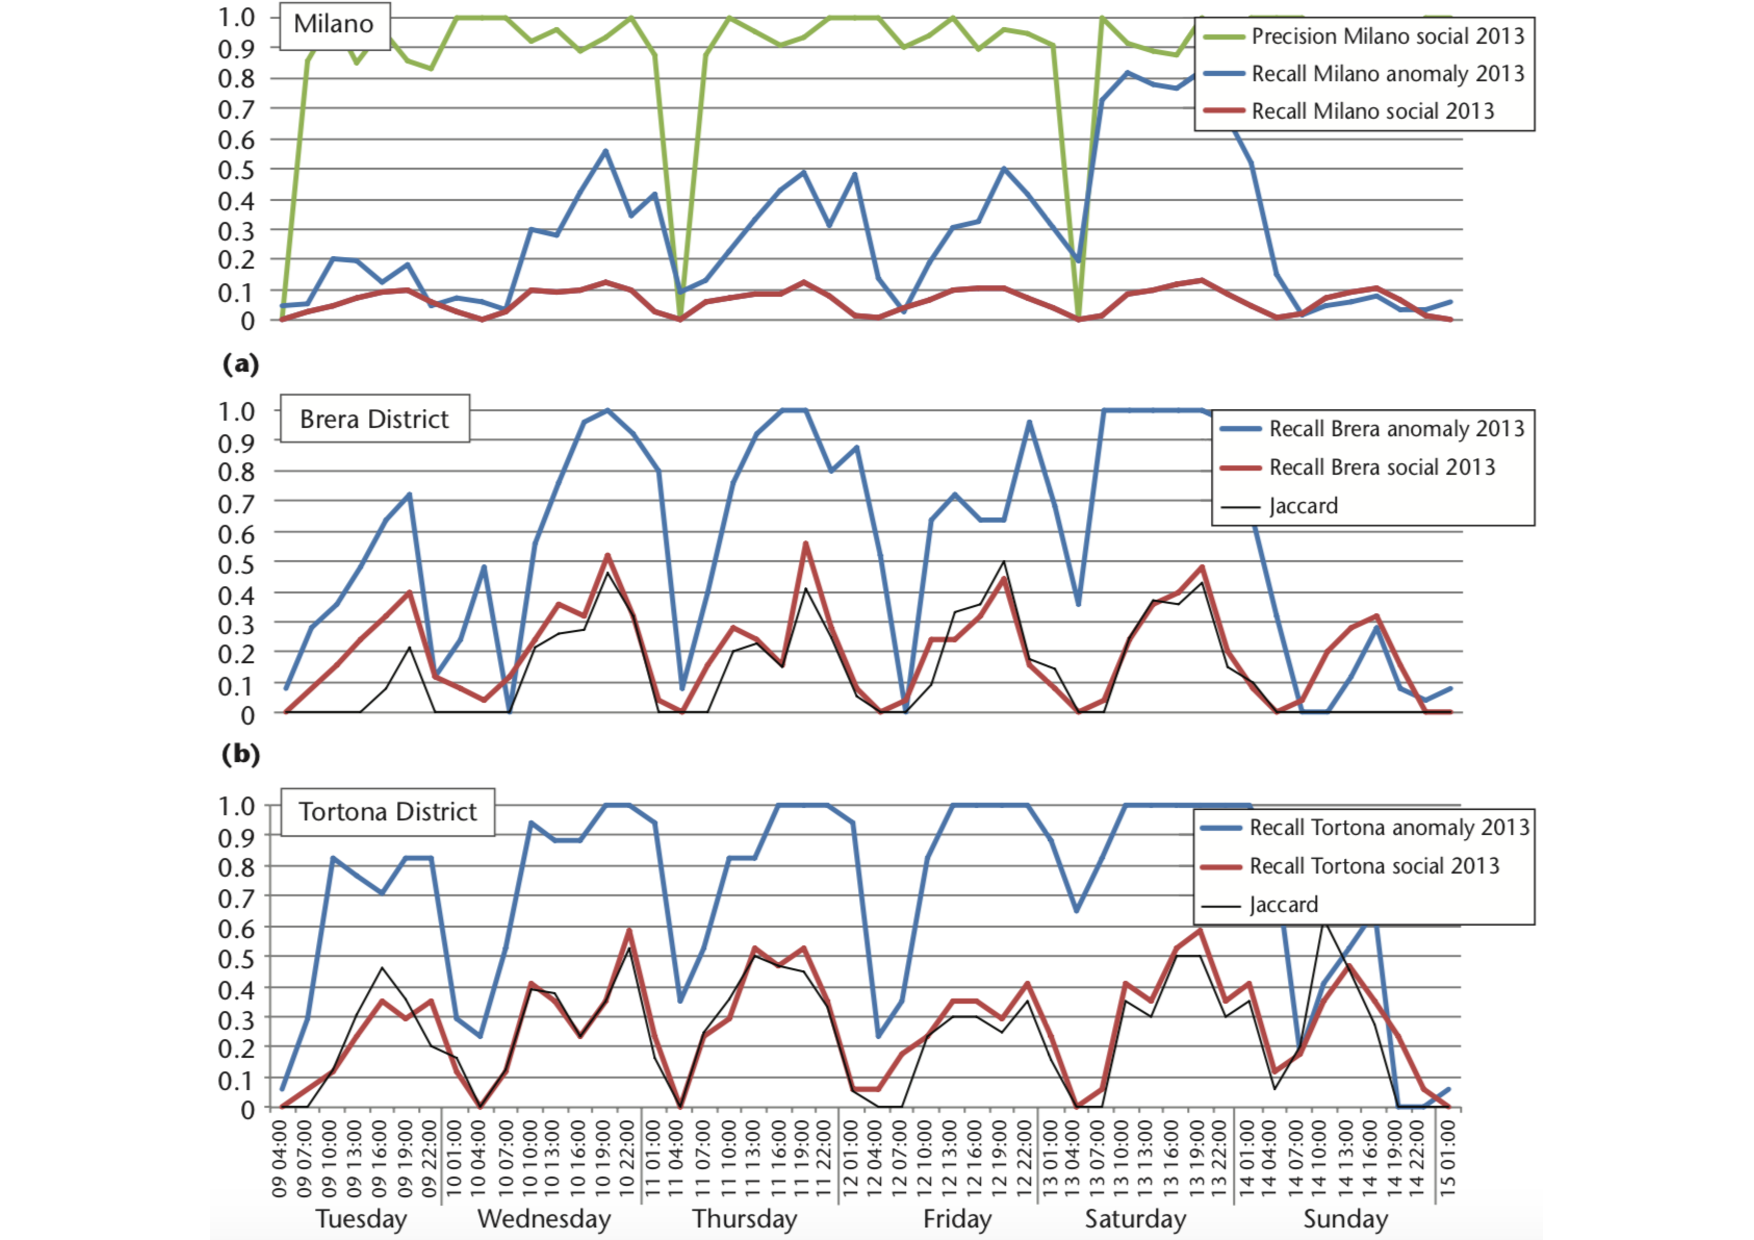
\includegraphics[width=0.90\textwidth]{img/mdw-prec-rec} 
\caption{Precision and recall of the social and mobile anomaly signals in identifying pixels where Milan Design Week (MDW) events happen in (a) Milano and the (b) Brera and (c) Tortona districts.}
\label{fig:mdw-prec-rec}
\end{center}
\end{figure}

We, then, created a gold standard (MilanP) consisting of all the pixels that contain at least one MDW2013 place. We also created two subsets of this gold standard (BreraP and TortonaP) that focus on the pixels that belong to the districts of Brera and Tortona, where the most important events were located. 
For each frame, we measured the ability of the social and mobile anomaly signals in identifying pixels in MilanP, BreraP, and TortonaP (see Figure~\ref{fig:mdw-prec-rec}) measuring precision and recall.

The results of the analysis show that the social signal has high precision (between 0.8 and 1 for 95 percent of the frames) in identifying pixels in MilanP. Its recall is low in identifying pixels in MilanP, but it is good (above 0.4 for around 60 percent of the frames) in identifying pixels in BreraP and TortonaP. In all cases, the signal volume is low: the average number of microposts linked to MDW per hour is 15 for MilanP, three for BreraP, and five for TortonaP.
However, the social signal is correlated to the anomaly index signal (see Figure~\ref{fig:mdw-prec-rec}) during the working days. The Pearson correlation for MilanP is 0.61 with a p-value of 2x$10^{-4}$ for BreraP, it is 0.76 with a p-value of 4.6x$10^{-7}$; and for TortonaP, it is 0.56 with a p-value of 3.1x$10^{-5}$. 

Moreover, not only the two signals are correlated, but they also identify the same pixels. To measure this, we computed the Jaccard similarity coefficient\footnote{The Jaccard coefficient measures similarity between finite sample sets} between the pixels identified by the social signal and those identified by the mobile anomaly signal. 
As we can observe in Figure~\ref{fig:mdw-prec-rec}, the Jaccard similarity coefficients in Brera and Tortona almost constantly overlaps with the recall of the social signal -- that is, if a pixel is identified by the social signal, then it's among those identified by the mobile anomaly signal.

%As a last step in understanding the data, we analyzed the graph that links people, places, and events. Similar to many other graphs describing real-world phenomena, it is scale-free~\cite{price1976general}. The frequency with which places, events, and hashtags of MDW are co-mentioned by people in microposts almost perfectly fits a power law ($y=12289x^{-1.832}$ with $R^2=0.96173$). For this reason, we draw the hypothesis that this information is best visualized using a graph~\cite{bertin1983semiology} where users are nodes, and links between two nodes represent discussions about the same place or event.

The data analysis phase (see phase~3 of the reference architecture presented in Section~\ref{sec:comp-mod-sol-arch}) bring evidences that: (i) Telco Big Data can provide a very relevant and dynamic overview of the presence of people in the context of a specific city or territory, aggregated at the level of the single cell tower, and (ii) Social data represent a precious source to build the interaction graph between people, events and places. 
However, since building the morphology of the territory can impact on the effectiveness of the cells, the CDR information can describe the city's dynamics at the macro level, but it cannot be used to precisely represent such dynamics at the micro level, e.g. input/output flows into one specific street or square. The social data, thanks to its public content and the precise location of each message, can help in filling this gap.

\subsection{MDW2014 - CitySensing Public Installation} \label{sec:cs-mdw-2014}
During the Milan Design Week 2014 (MDW2014), exploiting the knowledge acquired analyzing the previous edition, we use \sti{} and \hivedi{} to realize the proposed CitySensing platform to collect and analyze social and telecommunication data. 
The visualization, enabled by CitySensing, is presented in a public installation in Mediateca Santa Teresa\footnote{\url{http://www.mediabrera.it/index/index.php}}.

During the MDW2014, we consider 21,782 micro-posts from Twitter and Instagram, data describing MDW2014 places and events from three heterogeneous sources (fuorisalone.it, breradesigndistrict.it, and tortonaroundesign.com), and Telecom Italia's CDRs (19,719,629 calls, 20,240,485 SMSs, and 197,767,245 Internet data accesses counted in the Milan area from 8 to 14 April 2014).
\hivedi{} analyze calls/sms/internet-accesses in real-time by aggregating them for each pixel and for each frame and by computing how anomalous they are comparing each of them against the predictions of the Gaussian models built at set-up time. 

As detailed in~\cite{DBLP:journals/ieeemm/BalduiniVALAC15}, the anomalous pixels correspond with high precision to pixels in which events of the Milan Design Week are happening. This allows us to provide experimental evidence that the extra 400,000 people that come to Milano for the Design Week generate extra calls/sms/internet-accesses from the cells that contain the 600 locations of the 1,200 Milan Design Week events.

To process social streams, we use \sti{} (see Section~\ref{sec:comp-mod-impl-v}). The original data stream are injected in \sti{} in Activity Stream 2.0 format\footnote{\url{http://www.w3.org/TR/activitystreams-core/}}. \sti{} semantically augments them using our custom Named Entity recognition and linking solution tailored on Milan Design Week~\cite{DBLP:conf/semweb/BalduiniV13}. A continuous query captures a frame every 15 minutes counting the number of distinct hashtags and semantic entities present in the geo-referenced microposts for each pixel. The results of this continuous query is a stream modeled in \frappe{}.

\begin{figure}[t]
\begin{center}
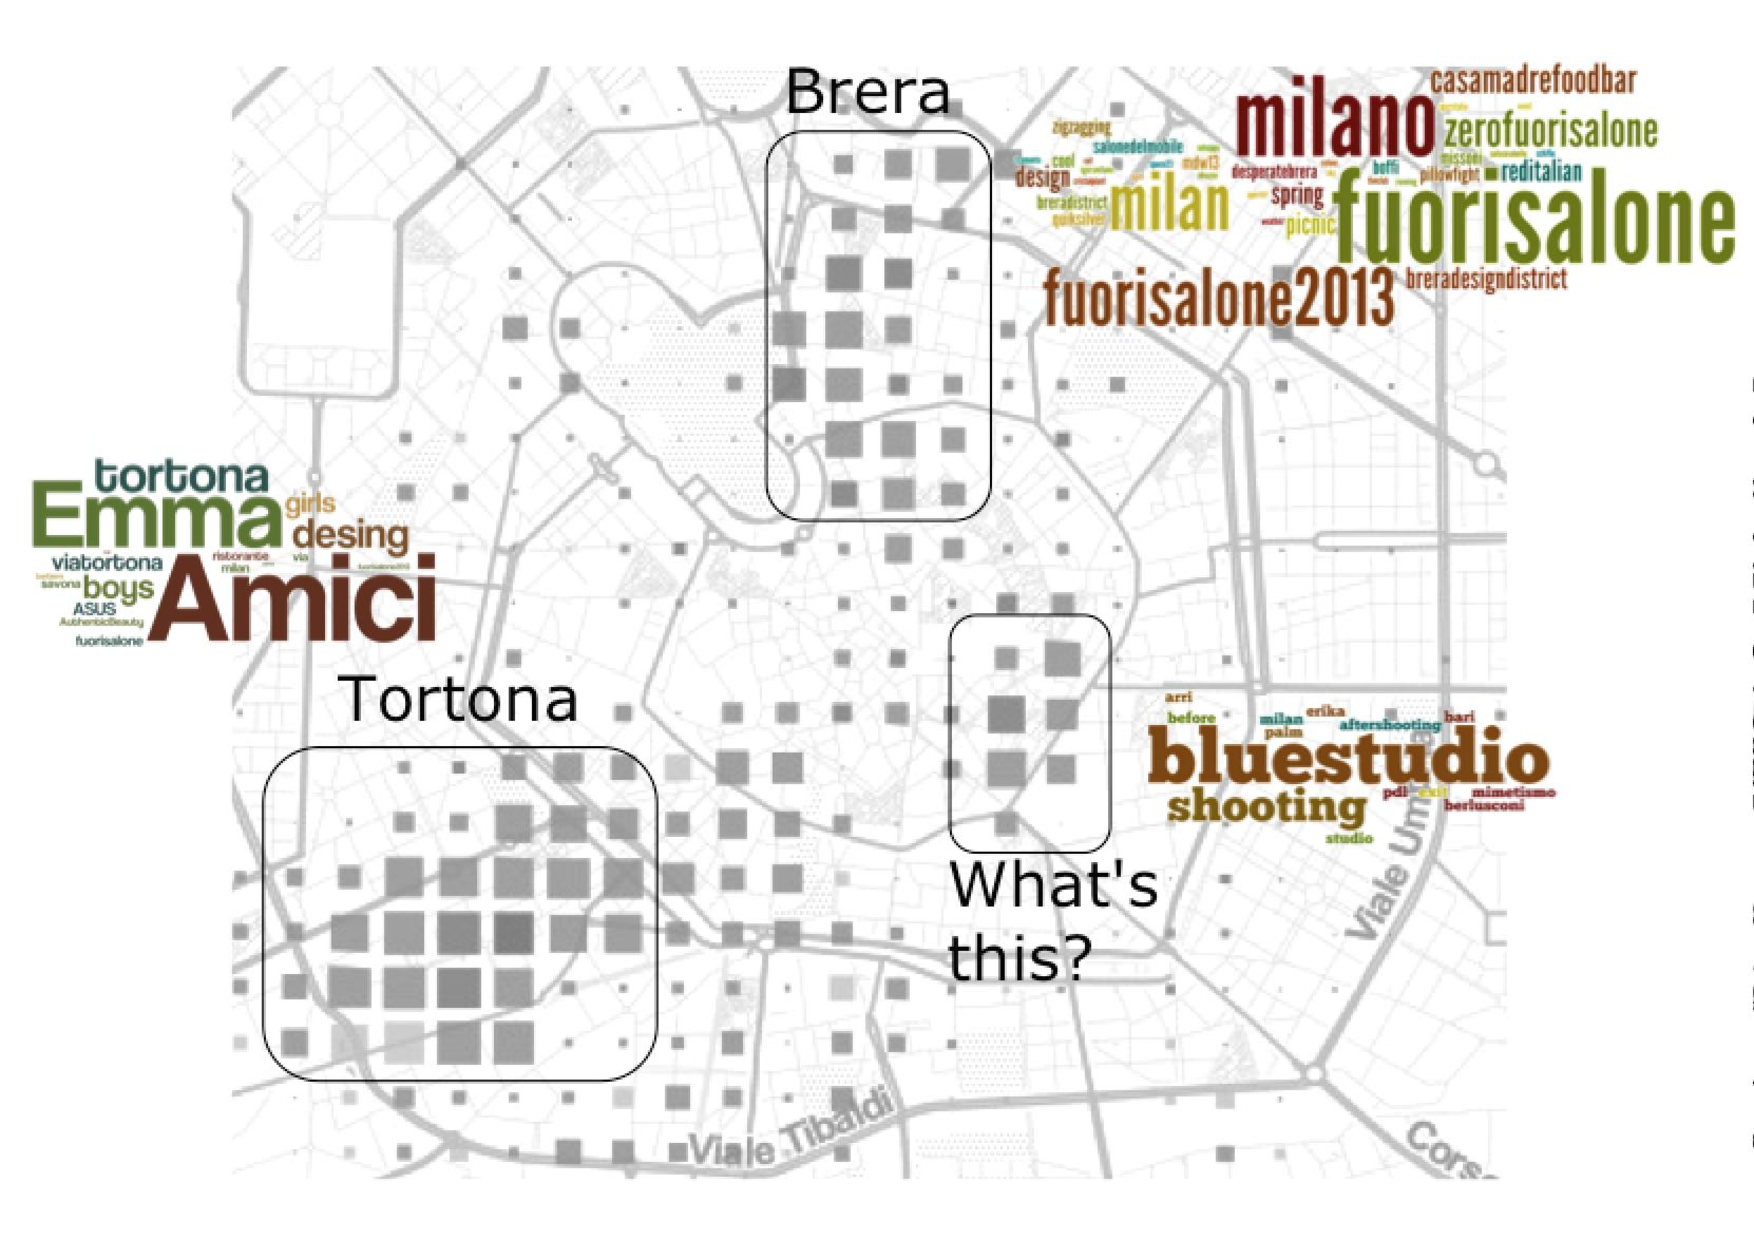
\includegraphics[width=0.49\textwidth]{img/mdw-ht-1} 
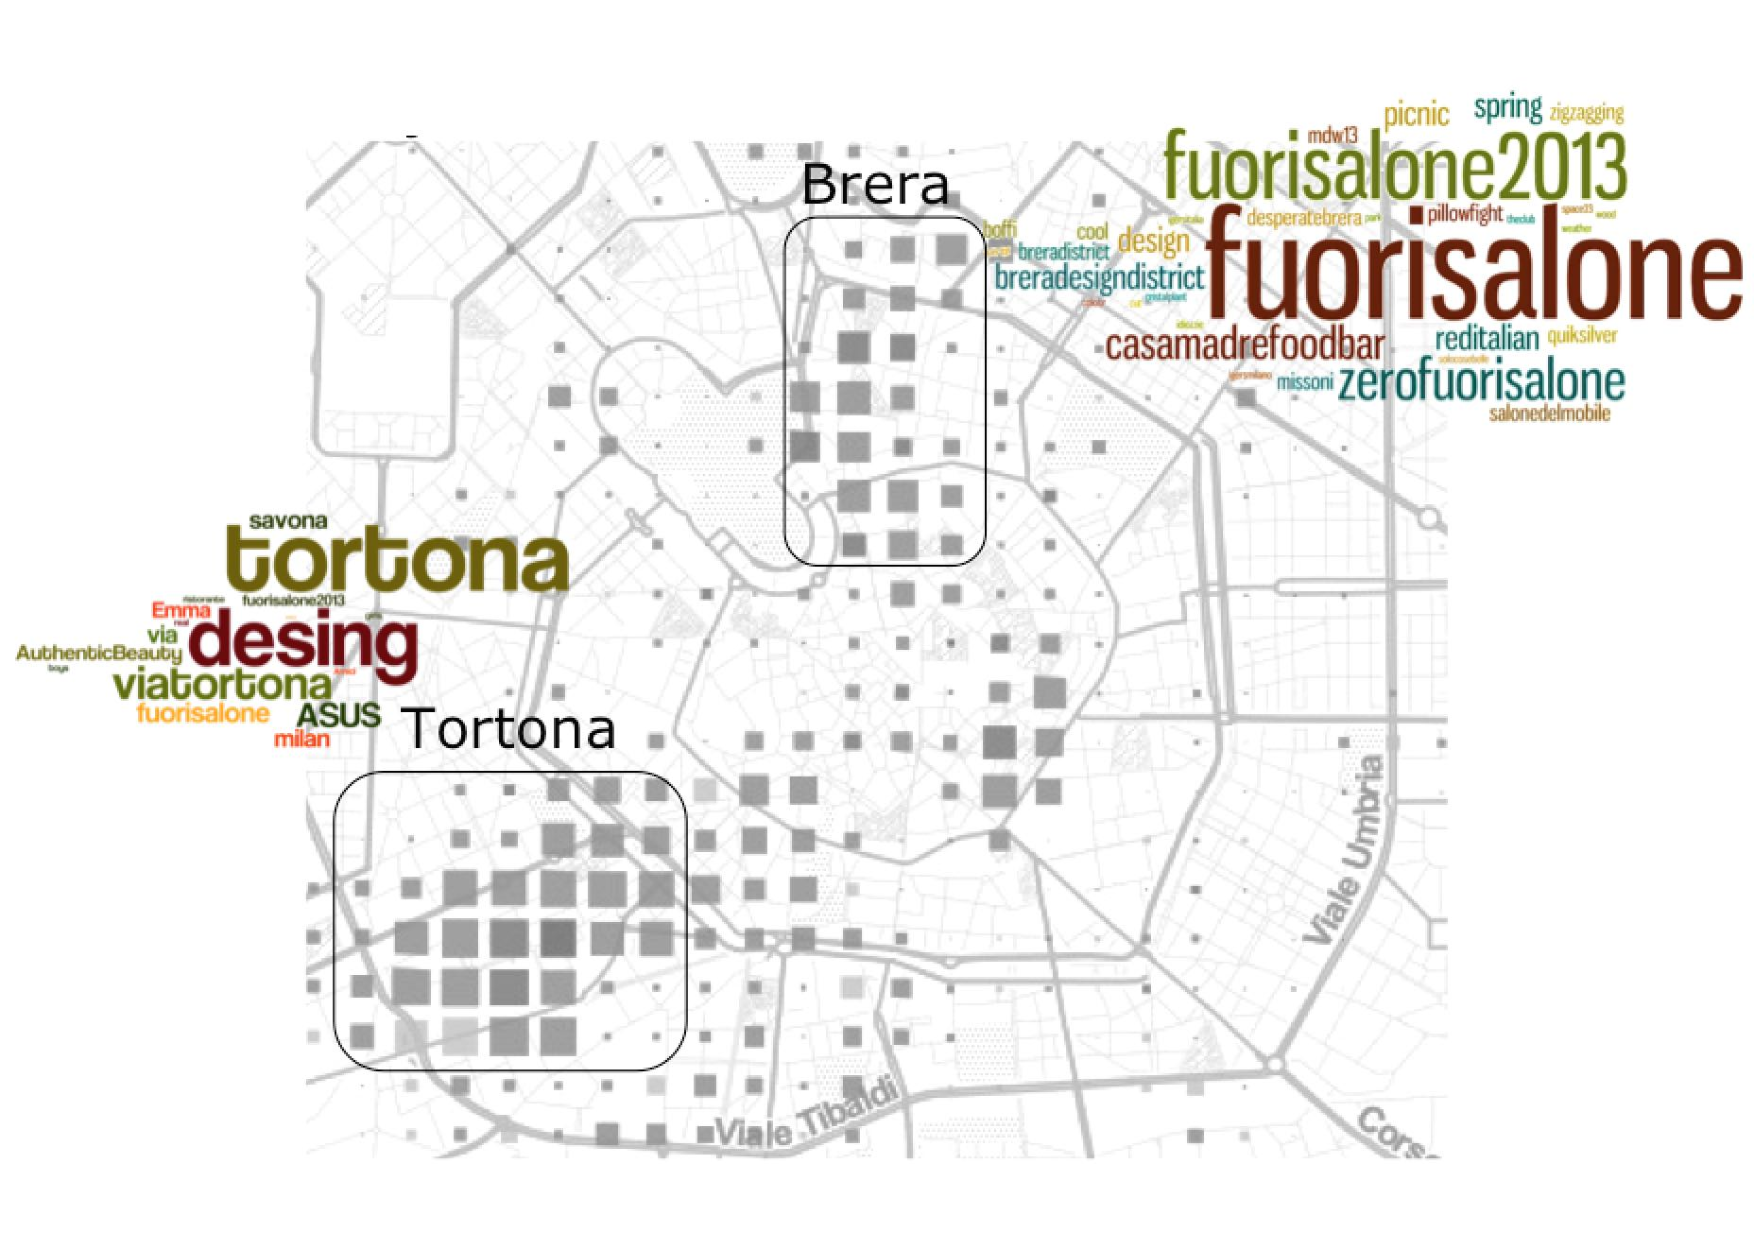
\includegraphics[width=0.49\textwidth]{img/mdw-ht-2} 
(a)\hspace{150pt} (b)
\caption{Social media used  to explain the reason of anomalous peaks of presence  in some pixels: (a) shows the most popular hashtags posted in the anomalous pixels during Milan Design Week, whereas (b) highlights the emergent hashtags, i.e., the non predicted ones. While the generic most popular tags contains also hashtag about a popular TV show (i.e., Amici or Emma), the emergent hashtags are those of Milan Design Week.}
\label{fig:de}
\end{center}
\end{figure}

As illustrated in Figure \ref{fig:de}.(a) a (partial) \textit{semantic} explanation of the mobile anomalies, can be attempted aggregating the top-10 hashtags used in those pixels. For instance, in Brera district the Italian hashtag of Milan Design Week (i.e., Fuorisalone) emerges. However, this technique is not dependable. For instance, in Tortona district also the hashtags of a popular TV show (i.e., Amici) and its protagonists (e.g., Emma) appear. Once again, the solution is in the ability to compare the current top hashtags against the those predicted by a statistical model. This allows highlighting only the emergent hashtags of this frame for the selected pixels  (see Figure~\ref{fig:de}.(b)).

\begin{figure}[t]
\begin{center}
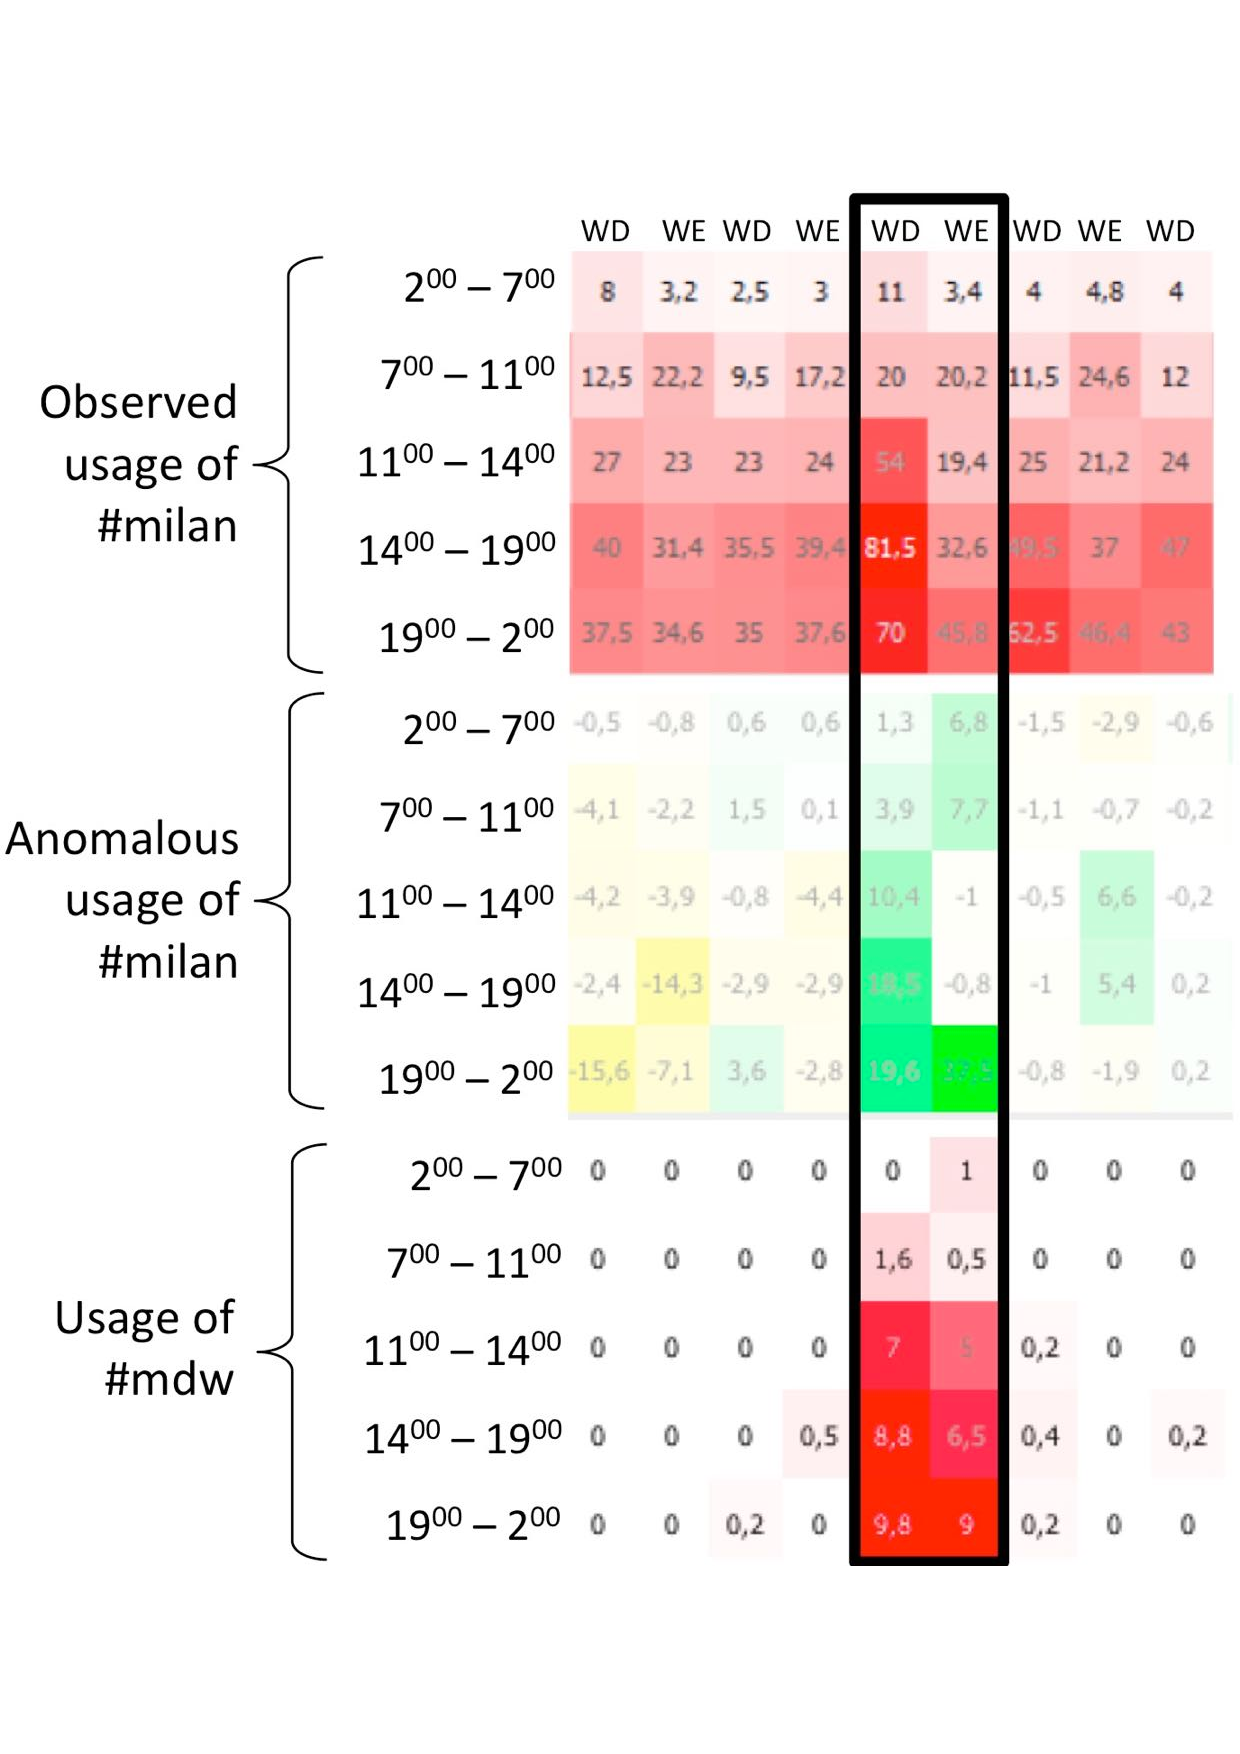
\includegraphics[width=0.5\textwidth]{img/mdw-ht-usage} 
\caption{Highlighting of anomalies in hashtag usage: The hashtag \#milan is used more often during the Milan Design Week.
Forecasting the \#milan time-series using Holt-Winter method, we were able to identify the anomalous usage, which is highly correlated to the usage of \#mdw -- the official hashtag of Milan Design Week. }
\label{fig:L}
\end{center}
\end{figure}

As one can expect, the simple Gaussian model used for the mobile activity is not appropriate to predict hashtag usage. We found, instead, that an Holt-Winter method can be used~\cite{kalekar2004time} to predict the usage over time of a specific hashtag (e.g., \#milan). In order to use Holt-Winter, we use \frappe{}: we build \textsf{SyntheticFrames} that aggregate the \textsf{CapturedFrames} in five parts of a day (i.e., 2am-7am, 7am-11am, 11am-2pm, 2pm-7pm and 7pm-2am). Moreover, as for the CDRs, we distinguish between working days and week-ends. This approach allows to build effective predictive models for hashtags about the points of interest of Milan and about popular TV shows. Figure \ref{fig:L} illustrates how this method detects the anomalous usage of \#milan during the Milan Design Week, which is highly correlated to the usage of  \#mdw -- the official hashtag of Milan Design Week.

During the Milan Design Week, using \sti{} to compare those models with the observed usage of an hashtag, we detect in real-time emerging hashtags. Figure~\ref{fig:L} illustrates how the extra usage of \#milan is correlated to the appearance of the official hashtag of Milan Design Week (i.e., \#mdw).

Using the analyses described above, CitySensing identifies pixels where people is talking about Milan Design Week. As detailed in Section~\ref{sec:cs-mdw-2013}, those pixels are not as numerous as those identified as anomalous using the CDRs. However, they match with almost absolute precision the pixels in which Milan Design Week events happen. The most interesting finding is that almost all those pixels are contained in mobile anomalous ones. This provides further experimental evidence that the anomalies observed in the CDRs are caused by the people coming to Milan for the Design Week.

The particular scheduling and geographical organization of the events of Milano Design Week, with most of the events concentrated in some specific areas of the city, enable also to perform analysis with irregular \textsf{grid}, based on the official areas of Fuorisalone.

% \begin{figure}[t]
% 	\begin{center}
% 		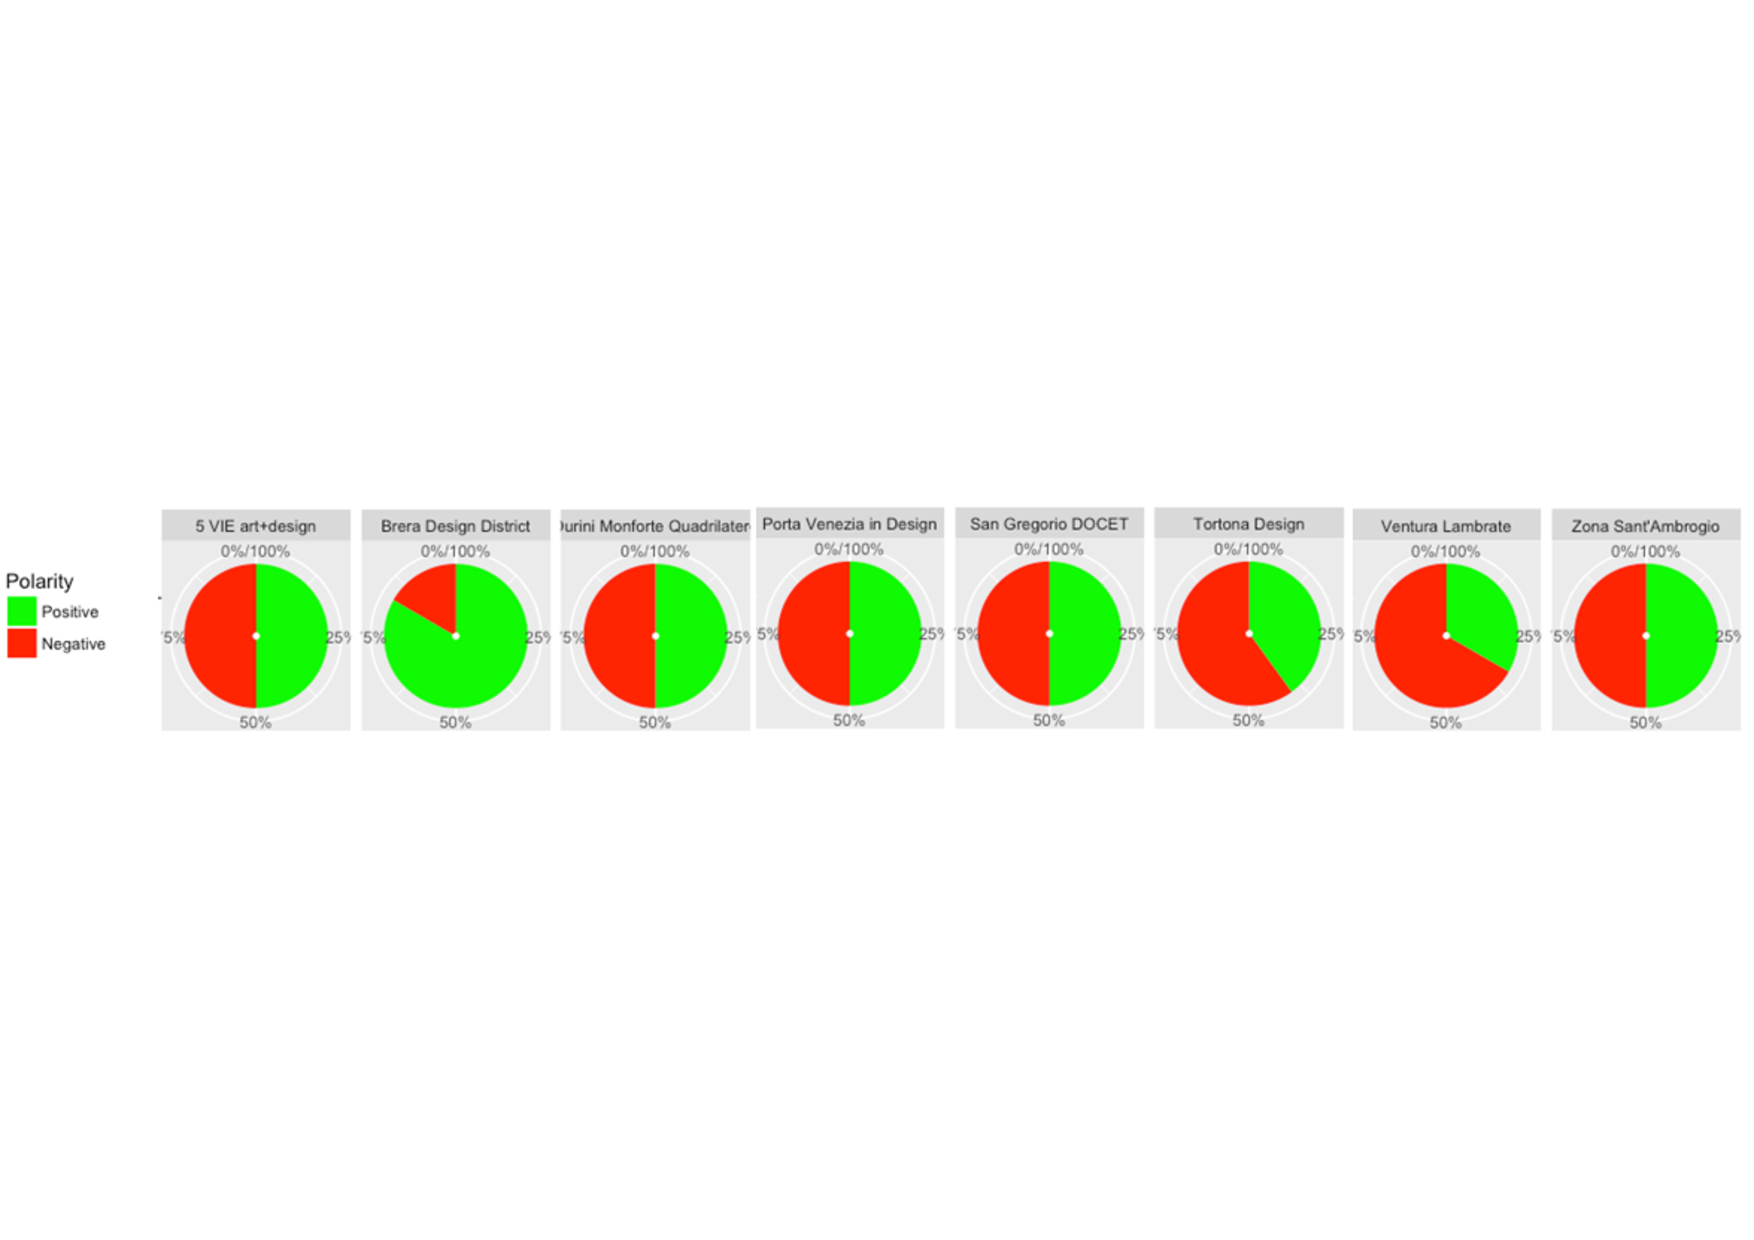
\includegraphics[width=\textwidth]{img/mdw-sentiment} 
% 		\caption{Share of positive and negative sentiment calculated for posts associated to the different MDW\ cells.}
% 		\label{fig:mdw_sentiment}
% 	\end{center}
% \end{figure}

%An examples of analysis performed on this grid is shown in Figure~\ref{fig:mdw_sentiment}, that represents the results of a semantical analysis on the text of tweets related to each area of Fuorisalone. We collect for each (irregular) \textsf{pixel} the tweets geolocated in some \textsf{place} of the \textsf{cell} and the tweets that speaks about the \textsf{event}s contained in the \textsf{pixel}, and we perform on them a semantical text analysis in order to extract the sentiment polarity of the text. Then we filtered neutral tweets and we compare the number of positive and negative tweets in each \textsf{pixel} in order to show, for each daily \textsf{frame}, which \textsf{pixel}s (that corresponds to an official area of Fuorisalone) are most successful according to the opinions of social network users.

\begin{figure}[p]
\centering
\subfloat[]{
	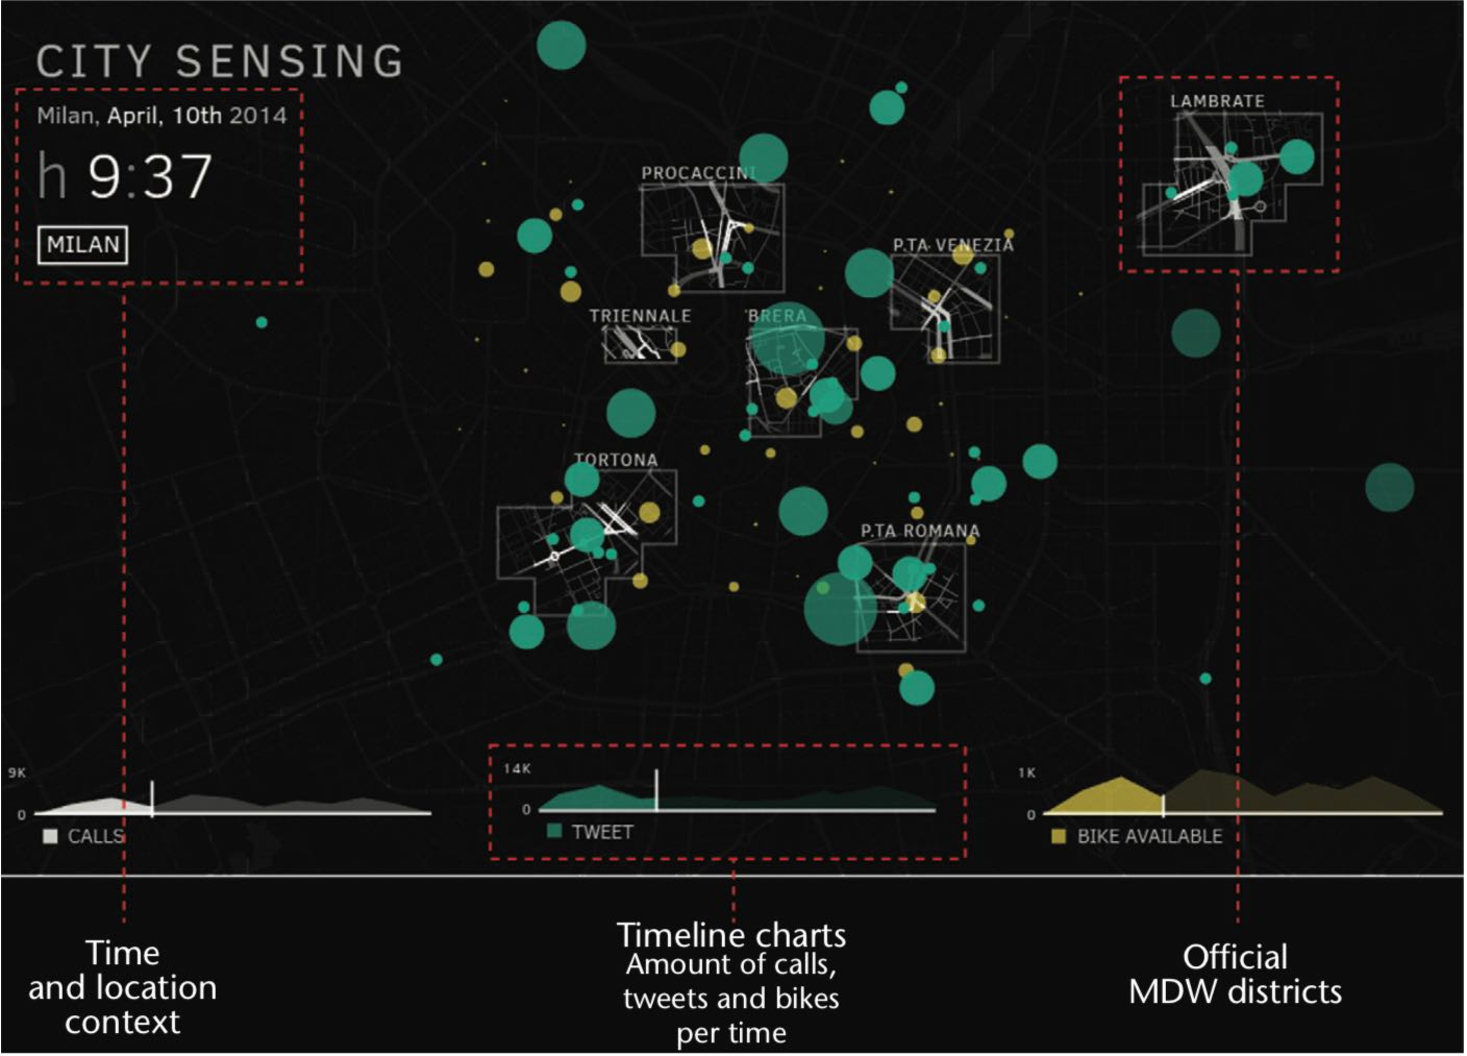
\includegraphics[width=0.52\textwidth]{img/mdw-vis-1} 
}\\
\subfloat[]{
	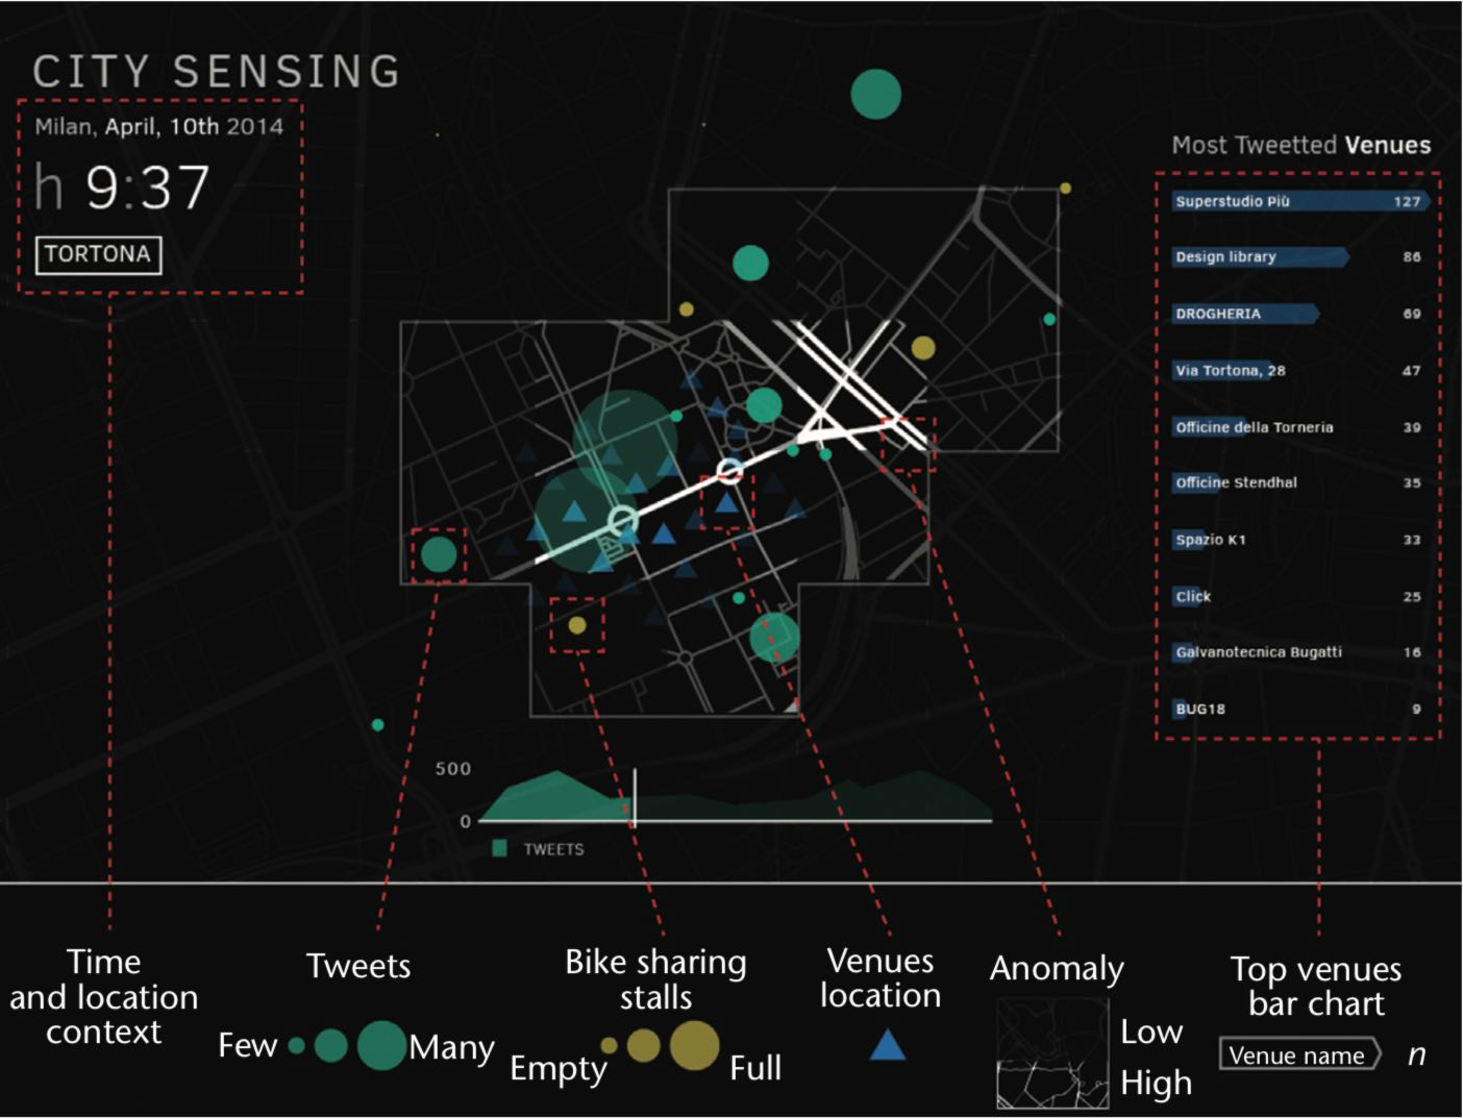
\includegraphics[width=0.52\textwidth]{img/mdw-vis-2} 
}\\
\subfloat[]{
    \includegraphics[width=0.52\textwidth]{img/mdw-vis-3} 
}
\caption{MDW2014 CitySensing installation geographical view (a) at city level, where the visualization highlights the pixels of official MDW districts, and (b) at district level, the map is zoomed and centered on the district. (c) The graph view displays the evolution of the graph of people visiting MDW2014 places and events. (source~\cite{DBLP:journals/ieeemm/BalduiniVALAC15}).}
\label{fig:mdw-2014-vis}
\end{figure}

% \begin{figure}[t]
%   \begin{minipage}{.33\textwidth}
%       \centering
%       \includegraphics[width=0.3\linewidth]{img/mdw-vis-1}
%   \end{minipage}
%   \begin{minipage}{0.33\textwidth}
%       \centering
%       \includegraphics[width=0.3\linewidth]{img/mdw-vis-2} 
%   \end{minipage}
%   \begin{minipage}{0.33\textwidth}
%       \centering
%       \includegraphics[width=0.3\linewidth]{img/mdw-vis-3} 
%   \end{minipage}
%   \caption{(a) MDW2014 CitySensing installation geographical view (a) at city level, where the visualization highlights the pixels of official MDW districts, and (b) at district level, the map is zoomed and centered on the district. (c) The graph view displays the evolution of the graph of people visiting MDW2014 places and events. (source~\cite{DBLP:journals/ieeemm/BalduiniVALAC15}).}
%   \label{fig:mdw-2014-vis}
% \end{figure}

% \begin{figure}[!t]
% \centering
% \minipage{\textwidth}
%   \includegraphics[width=0.5\linewidth]{img/mdw-vis-1}
% \endminipage\hfill \\
% \minipage{\textwidth}
%   \includegraphics[width=0.5\linewidth]{img/mdw-vis-2}
% \endminipage\hfill \\
% \minipage{\textwidth}
%   \includegraphics[width=0.5\linewidth]{img/mdw-vis-3}
% \endminipage
%  \caption{(a) MDW2014 CitySensing installation geographical view (a) at city level, where the visualization highlights the pixels of official MDW districts, and (b) at district level, the map is zoomed and centered on the district. (c) The graph view displays the evolution of the graph of people visiting MDW2014 places and events. (source~\cite{DBLP:journals/ieeemm/BalduiniVALAC15}).}
%  \label{fig:mdw-2014-vis}
% \end{figure}

The CitySensing visualizations exploit the \frappe{} concepts to relate time and space.
They comprise two main views: a geographical view (see Figures~\ref{fig:mdw-2014-vis}(a) and \ref{fig:mdw-2014-vis}(b)) that displays signals on a static map of Milan, and a graph view (see Figure~\ref{fig:mdw-2014-vis}(c)) that displays the evolution of the graph of people visiting MDW2014 places and events. Both can be zoomed in at the city or district level. The system underpinning the views enables the story to be told in nearly real time, but the visualized phenomenon is better viewed quickly, with the system playing a day in few minutes. To this end, a new frame, which aggregates 15 minutes of data, is displayed every 2 seconds\footnote{\url{http://citysensing.fuorisalone.it}, \url{http:// youtu.be/MOBie09NHxM}}.

Finally, we perform an empirical evaluation of \frappe{} in order to understand how the CitySensing visualizations ease the attendees' understanding of data dynamics and, consequently, validate the \textsf{Hp.3}. 

\begin{figure}[p]
\centering
\subfloat[]{
        \includegraphics[width=.63\linewidth]{img/mdw-vis-4}
}\\
\subfloat[]{
        \includegraphics[width=.63\linewidth]{img/mdw-vis-5}
}\\
\subfloat[]{
        \includegraphics[width=.63\linewidth]{img/mdw-vis-6}
}
\caption{(a) The correlation between the social and mobile anomaly signals is readable in the story told by the geographical view at city level. On 10 April 2014, the social and mobile anomaly signals tell the success of MDW districts: Brera and Tortona beat all others. (b) A geographical view in which the social and mobile anomaly signals tell the daily pattern of activity in Brera. (c) This graph view highlights the scale-free nature of the graph of people when connected by the places, events, and hashtags they discuss on social media. (source~\cite{DBLP:journals/ieeemm/BalduiniVALAC15}).}
\label{fig:eval-empirical}
\end{figure}

We start from the author-driven perspective, illustrating the visualizations as the people who watched the installation in Mediateca Santa Teresa experienced them. Then, we take the reader-driven perspective and report on the results of a questionnaire meant to assess whether the audience could guess the visualizations' intended message.

Figure~\ref{fig:eval-empirical}(a) illustrates how the correlation between the social and mobile anomaly signals is readable in the story told by the geographical view at the city level. The figure represents a cumulative view of the frames between 6:00 and 24:00 on 10 April (the most active day in 2014). The majority of the streets of MDW districts "spot out" that is, the pixel highlighted by the mobile anomaly signal are MDW places. Furthermore, a clear pattern emerges: the MDW social signal (the green circles) originates from MDW districts.

Figure~\ref{fig:eval-empirical}(b) presents the geographical view, but it focuses on the Brera district. This view illustrates the evolution of the social and mobile anomaly signals over three frame groups (06:00--12:00, 12:00--18:00, and 18:00--24:00) on 10 April 2014. The places where MDW events are held normally open in the late morning, but the majority of the events start in the afternoon. This is clearly visible both in the value of the mobile anomaly signal (mapped to the opacity of the pixels) and the volume of the social signal (mapped in the size of the green circles): both signals increase in most of the pixels and especially in those containing MDW places (blue triangles).

Figure~\ref{fig:eval-empirical}(c) illustrates the graph view. It shows the evolution of the same three frame groups on 10 April 2014. During the morning, few users are linked by topics related to MDW; in the afternoon, a cluster of people talking about places and events of MDW appears; and in the evening, just few users remain unlinked. This is a direct consequence of the long-tail distribution of the discussion topics: 80 percent of the users talk about 20 percent of the places/events, while the remaining 20 percent of the users talk about the other 80 percent of places/events.

This pattern repeats over the days at city scale and in the Brera and Tortona districts. It disappears when MDW ends.
To verify the \textsf{Hp.3}, we asked people without specific skills in data visualization and analytics to guess the message of the views shown in Figure~\ref{fig:eval-empirical}(a)~and~\ref{fig:eval-empirical}~(c). We asked them the six questions reported in Figure~\ref{fig:eval-empirical-quest}. In four cases, we asked true-or-false questions, and in two cases, we asked questions that had no correct answer (see "uncertain" in the figure). The correct answers are underlined in Figure~\ref{fig:eval-empirical-quest}. As the distribution of the answers of the 23 responders shows, the messages we intended to transmit were correctly guessed. The responders correctly correlated the social and the mobile anomaly signals when the correlation was not evident and could not guess the correct answer when the correlation was not present. The same happens when they guess the meaning of the graph that links people based on the places and events that they jointly discussed.
Those results validate Hypothesis~\textsf{Hp.3}.

\begin{figure}[t]
\centering
\includegraphics[width=.9\linewidth]{img/mdw-vis-7}
\caption{The results of the questionnaire about the visualizations presented in (a) Figure 5 and (b) Figure 7. As we can see from the distribution of the answers of the 23 responders, the messages we intended to transmit (underlined) were correctly guessed. (source~\cite{DBLP:journals/ieeemm/BalduiniVALAC15}).}
\label{fig:eval-empirical-quest}
\end{figure}

\subsection{MDW2016 - Advanced Visualizations} \label{sec:cs-mdw-2016}
Comforted by the guessability level of the CitySensing visualization, we try to reach an higher level of complexity in the data presentation.
During the 2016 edition of the event we had the opportunity to collect data coming from an additional relevant source: the official mobile application of Fuorisalone. In particular, we had access to the GPS positions of \textsf{place}s where the users open the App and the \textsf{event}s inserted in the agenda on the App. Also, in this context, we apply the method of squared \textsf{grid} tessellation of the city, in order to analyze the correlation between pairs of different signals.

The Figures~\ref{fig:gps_geo_1} and Figures~\ref{fig:gps_geo_2} depicts the results, obtained exploiting \frappe{}, \sti{} and \sparkdi{}, of different use cases that involves data from heterogeneous sources (i.e., GPS record of the usage of the official Fuorisalone App, public social network, official schedule of Fuorisalone events).

\begin{figure}[p]
\centering
\subfloat[]{
	\includegraphics[width=0.75\textwidth]{img/mdw-gps-events} 
} \\
\subfloat[]{
	\includegraphics[width=0.75\textwidth]{img/mdw-gps-geo} 
}
\caption{The Figure (a) shows the number of Mobile App GPS observations collected in one day inside each square
of the grid (red dots) correlated with the number of events of Milano Design
Week scheduled for the same day in the same square. The Figure (b shows the correlation between GPS observations (red dots) and geo-located posts on social networks (blue dots) inside each square.}
\label{fig:gps_geo_1}
\end{figure}

Figure~\ref{fig:gps_geo_1}(a) shows the correlation between the use of the App and the number of Fuorisalone events. To visualize such a phenomenon, we consider as \textsf{event}s the use of the App in a \textsf{place}, that generates a GPS record, and the scheduled \textsf{event} of MDW with their \textsf{place} that users put in their agenda. Data is aggregated grouping by \textsf{Pixel}s and capturing daily \textsf{Frame}s.

Another available source of \textsf{Event}s is the geo-located activity on the public social networks: we collect the Twitter and Instagram posts geo-located in the \textsf{Place}s contained in each \textsf{Cell} and we aggregate them gropuping by \textsf{Pixel}s containing the GPS observations, as shown in Figure~\ref{fig:gps_geo_1}(b).
Both \textsf{Frame}s show the increasing of the \textsf{Event}s in the areas of the Fuorisalone.

\begin{figure}[p]
\centering
\subfloat[]{
    \includegraphics[width=0.75\textwidth]{img/mdw-euro-us-visitors} 
}\\
\subfloat[]{
    \includegraphics[width=0.75\textwidth]{img/mdw-italian-visitors}
}
\caption{ The Figure presents (a) the localization of the five largest groups of European and US visitors and (b) Italian visitors.}
\label{fig:gps_geo_2}
\end{figure}

Another interesting use case is represented by the analysis of the provenance of the visitors during the Milano Design Week.
In order to estimate the provenance of the visitors we use the GPS information collected by the App, extracting the GPS position of the first observation logged for each user before the days of the MDW (assuming that the users download the App at home). Using appropriate shape files we map each GPS location to a Country in the world, obtaining the provenance of the user.

Mapping the GPS observation \textsf{event}s in the \textsf{grid} of \textsf{pixel}s, it is possible to visualize, for each daily \textsf{frame} and for each people group, which are the most popular areas of the city. Figure~\ref{fig:gps_geo_2}(a) shows the localization of the five largest groups of European foreign visitors and United States visitors. Figure~\ref{fig:gps_geo_2}(b) shows the region of provenance of Italian visitors and their distribution in the events.

As for the public installation during MDW2014, we test the guessability of the advanced visualizations.
The new advanced visualizations are created for a more professional audience (i.e. Studiolabo\footnote{http://studiolabo.it/}, the main organizer and stakeholder of Fuorisalone).
A user-centric study we conducted observing how Studiolabo used the visualizations during a workshop, allowing us to affirm that our stakeholder was able to understand the visualizations and exploit the analysis results.
Therefore, these empirical evaluation of the MDW2016 visualizations enforces the validity of Hypotheses \textsf{Hp.3}.

\section{Milano Fashion Week} \label{sec:cs-mfw}
The Milano Fashion Week (MFW) represents another example of CSE in Milan. This experience deals with the problem of understanding the social media response of the MFW  occurred from the 24$^{th}$ to the 29$^{th}$ February of 2016.
We use \sti{} to analyze the behavior of users who re-acted (or pro-acted) in relationship with each specific fashion show during the week. MFW represents the most important meeting between market operators in the Italian fashion industry. Out of the 170 shows, we are interested only in the catwalk shows, which are the core of the fashion week. The whole set of catwalks includes a total of 73 brands; among them, 68 brands organize one single event, 4 brands organize 2 events, and 1 brand organizes 3 events. 

\begin{figure}[p]
\centering
\subfloat[Granger Causality tests result]{
	\includegraphics[width=.85\linewidth]{img/mfw-trend}
}\\
\hspace{5pt} 
\subfloat[Density of posts]{
	\includegraphics[width=.65\linewidth]{img/mfw-map}
} 
\caption{(a) Granger causality test curves between physical events and social media response of each brand during the MFW, clustered by similarity of behavior; (b) Geographical dispersion over the cells of physical events (red stars)
and density of social media activity (blue).}
\label{fig:fashion_fig}
\end{figure}

We initially extract posts by invoking the social network APIs of Twitter and Instagram; for identifying the social reactions to MFW, we use a set of 21 hashtags and keywords provided by domain experts in the fashion sector, i.e., researchers of the \textit{Fashion in Process} group (FIP) of Politecnico di Milano\footnote{\url{http://www.fashioninprocess.com/}}.
We focused on 3 weeks: the one before, the one after and the one of the event. In this way, \sti{} and \hivedi{} collected 106K tweets (out of which only 6.5\% geo-located) and 556K Instagram posts (out of which 28\% geolocated).
Eventually, we opt for considering only Instagram posts, as they represent a much richer source for the particular domain of Fashion with respect to Twitter~\cite{Brambilla2017, BrambillaSpatial2017}.

We model the data using \frappe{} and exploit \sti{} and \hivedi{} to enable temporal, spatial and content analyses on the modeled information.
Following the \frappe{} approach, we build a regular \textsf{Grid} of \textsf{cell}s above the area of Milan, and assigned each post to the appropriate \textsf{Cell}. The \textsf{Grid} has a square shape, with sides of $10km$, divided into 20 rows and 20 columns, for a total of 400 \textsf{Cell}s of $500m \times 500m$. 

According to the \frappe{} model, an \textsf{Event} is organized by a brand at time $\tau_{n}$, hosted in the \textsf{Place}, located the \textsf{Cell} of a \textsf{Grid}. Each \textsf{Cell} is related to a \textsf{Pixel} and the \textsf{Grid} is captured by a \textsf{CapturedFrame}. An \textsf{Agent} (a user) may contribute with some \textsf{OriginalContent} (e.g., Instagram post), related to an \textsf{Event}, which in turn is going to be augmented by an automated enriching and analysis process that may add entities, as well as extract visual properties (color, pattern, ...) and concepts (objects, people, ...) from posted images.

We extend \frappe{} with \textsf{FrameLevelSynthesis} and \textsf{PixelLevelSynthesis} activities in order to represent the augmentation activities on the \textsf{OriginalContent}. We also add further concepts to \frappe{}.
We name \emph{Alive pixels} those where the percentage of posts shared in the considered pixel is more than $1\%$ of the total number of posts in the frame. We name \emph{Active pixels} those where the percentage of posts shared in the considered pixel is more than $10\%$ of the total number of posts in the frame. We name \emph{Strongly Active pixels} those where the percentage of posts shared in the considered pixel more than $20\%$ of the total number of posts in the frame.
We compute the number of alive, active and strongly active cells for all brands; we also compute the differences between subsequent durations (e.g. 3h - 6h) by counting how many cells changed their state.

Our first goal is to perform a \textbf{temporal analysis} aiming at characterizing the time at which social media respond to the events which appear in the official calendar and are linked to specific brands. 
Exploiting frame level synthesis we observe either peaks of reactions which then quickly disappear, or instead slower reactions that tend to remain observable for a longer time. Estimating the time latency of social responses to events is important for the brands, which could reactively plan more accurate reinforcement actions, essentially by adding well-planned social actions so as to sustain their social presence over time. We run Granger causality for each brand to compare the physical events and the social media reaction, and then we exploite k-means algorithm to cluster the brand by similarity of the Granger curves.
Figure \ref{fig:fashion_fig}(a) shows the clusters of Granger causality curves of the brands.

Our second goal is to \textbf{analyze the geographical dispersion} of social media response. We have two different spatial signals: (i) the calendar events; and (ii) the volume of social media posts on the Web with geographical information attached, i.e., latitude and longitude. Given these two signals, several features can be computed in order to describe the spatial dispersion of posts following an event. 
We compute different measures that reflect the dispersion of the social media signal over time, using: \emph{Gini coefficient}, \emph{Average distance} of the social media signals from the event location, and the number of \emph{alive}, \emph{active} and \emph{strongly active} cells.
Figure~\ref{fig:fashion_fig} (b) shows the  map representing the geographical distribution of events (represented by red stars) and post density using a synthetic frame where the pixel are darker where the density is higher.

The final result of the analysis is a set of advanced visual interfaces to be exploited by professional users.
The stakeholder (FIP), exploiting those visual interfaces, was able to observe that: (i) as the duration of the frame increases, the number of \emph{alive pixels} also increases. Moreover, the number of \emph{active} and \emph{strongly active pixels} is floating in the range from 1 to 3, with very few brands reaching 4 \emph{active pixels}. (ii) At the start of the event, posts are shared near the event location, but, as looking at the bigger picture, including 24 hours or even the entire period of 24 days, the \emph{average distance} is increasing, showing the growing dispersion of the social signal. (iii) The \emph{Gini coefficient} proves how the concentration of the social signal remains always high, due also to the fact that the low percentage of users that allows Instagram to geo-tag their own photo is reducing the number of authors implied in this study, and so the few authors with high volumes of posts generated are biasing the results. However, looking at the \emph{Gini alive coefficient}, which refers to the Gini coefficient computed only over the pixels that result alive for at least one brand in the specific frame, they can see a weak smoothing of the concentration strength with the increasing of the time-scope.

This proposed visual interfaces, based on \frappe{} concept (in particular, Frame and Pixel), result guessable and enable visual correlation of the presence of an event (stars) to the density of the social activity (darker pixels) over time.
The guessability of this visualizations validates, once more, Hypothesis \textsf{Hp.3}.

\section{Como Smart City for Smart Citizens} \label{sec:cs-como}
Como Smart City for Smart Citizens (ComoSC\textsuperscript{2}) is a big-data integration project started in 2016 where we involve the Municipality of Como and TIM-Telecom Italia. The purpose of the project is to create a system for the integration, analysis and interpretation of the large amount and heterogeneous data coming from different sources, in order to understand Como's urban dynamics and support  the decision making process of Como's local government.

\begin{figure}[t]
  \centering
  \includegraphics[width=.6\linewidth]{img/como-district}
  \caption{The seven irregular data-driven cells based on mobile phone data that cover the Como territory.}
  \label{fig:map1}
\end{figure}

As in MDW, we analyze the dynamics of \textbf{mobile phone traffic} (preventively anonymized and aggregated, according to privacy-preserving policies) in different areas of the city. 
Differently from the experiences in Section~\ref{sec:cs-mdw}~and~\ref{sec:cs-mfw}, in ComoSC\textsuperscript{2} we use \frappe{} with and irregular \textsf{Grid} composed by seven data-driven \textsf{cell}s built according to the distribution of the phone antennas and the characteristics of the area. 
We name those cells: historical city  center, lakeside promenade, touristic areas outside from the historical center, lake area, mountain area around the city, business and universities area, industrial outskirts.
The map in Figure~\ref{fig:map1} represents the distribution of the seven cells.

% One example is the comparison between the number of visitors from neighboring countries of Italy. 
% As depicted in Figure~\ref{fig:como_country_day}, Swiss people usually comes to Como for shopping on Saturdays in July while this trend dramatically decreases in September. 

\begin{figure}[p]
\centering
\subfloat[]{
        \includegraphics[width=.75\linewidth]{img/como-visit-july}
}\\
\subfloat[]{
        \includegraphics[width=.75\linewidth]{img/como-visit-summer}
}
\caption{(a)Number of foreign visitors per country per day in July in Como: Swiss, German, and French are the most present in the weekends. (b) Number of foreign visitors per country per day in Como from June to October. One can notice that Swiss visitors decrease sensibly in September.}
        \label{fig:como_country_day}
\end{figure}

We collect the mobile phone traffic data during several months, in particular we focuse on the summer period (from May to October 2016). Inside each \textsf{cell}, exploiting \sparkdi{}, we analyze the trend of mobile phone traffic capturing \textsf{frame}s with different duration (one hour, one day) and different coverage (the complete grid or a group of cells). 
Anonymized mobile phone data contains also information about the SIM (like international dial-code) and demographics information about the owner of the SIM (like gender or age-range).
As a result, we can perform analysis not only about the \textsf{event}s of people presence but also about the characteristics of people (\textsf{event content}) and to produce visualizations to ease the understanding of complex data.
For instance, Figure~\ref{fig:como_country_day} shows the comparison between the number of visitors from neighboring countries of Italy.
In particular Figure~\ref{fig:como_country_day}(a) shows the amount of visitors during the summer, while Figure~\ref{fig:como_country_day}(b) refers to July.

\begin{figure} [t]
        \centering
        \includegraphics[width=.8\linewidth]{img/como-hourly-distribution}
        \caption{Patterns of people presence in Duomo Square on working days and weekends: Tuesday, Thursday and Saturday are more crowded due to open market in the streets; Week ends are extremely crowded (including Saturday night).}
        \label{fig:duomo}
\end{figure}

Besides mobile phone data analysis, we instrumented the Cathedral Square of Como (\textit{Piazza Duomo}) with a set of \textbf{IoT (Internet of Things) sensors for counting people} passing in the square. The installation of the IoT sensors covers all the access to the square, and each sensor count how many people pass from the access every minute and push the results in real-time to \sparkdi{}.
We collect the data from IoT sensors and model it with \frappe{}.
Exploiting \textsf{CapturedFrames} with different time duration (hour, day and week), we construct the trend of passages \emph{from} and \emph{to} the Duomo Square according to the day of the week and the hour of the day (see Figure~\ref{fig:duomo}). 
This trend represents the starting point to analyze trending pattern and anomalies. 

The result of the analysis is a report containing an overview of the crowd movement around the city.
In order to validate Hypothesis \textsf{Hp.3}, we organized a workshop for the data analysis team of the Municipality of Como.
Exploiting the report on the analysis of mobile traffic data, the analysts were able to identify particular trends. For instance, the analysis of Figure~\ref{fig:como_country_day} shows that Swiss people usually comes to Como for shopping on Saturdays in July, but this trend dramatically decreases in September.
Moreover, exploiting the passage trend analysis, the team, identifies two different patterns of people presence in Duomo Square: one for working days and one for weekends, with a significant increase of people during Saturdays and Sundays, with respect to working days.
More in details, they found some differences inside the two patterns. For example in week-ends clearly emerge a difference during the evenings: Saturday evening shows a sort of persistence of people presence, while Sunday evenings appear more similar to working-day evenings. Another significant difference is the increase of people presence on Tuesday and Thursday mornings, with respect to the other working days. They are significant because the local market activities in the square during such mornings induces higher flows than usual.

The report eases the access to the results and is exploited by the Municipality of Como to enable decision making process to change the urban aspect of the city center (i.e,  the creation of a new pedestrian zone).
Once again, we collected experimental evidence that the \frappe{} approach, together with the \sparkdi{} implementation of \river{}, enables a series of different analytics on data streams characterized by high variety.
The understandability of complex data and the enabled decision making process validate Hypothesis \textsf{Hp.3}.

\section{Conclusion} \label{sec:cs-conclusion}
In this section, we conclude the chapter by showing the correlation of the case studies with: (i) the adoption and the evolution of the \frappe{} concepts, and (ii) the implementation of \river{} that better fits the analytics needs.
Table~\ref{tab:frappeAnalysis} proposes an analysis of how important each of the \frappe{} concept is in the various experiments and shows the extendibility of \frappe{}, while Table~\ref{tab:techAnalysis} shows which implementation of \river{} is used in the various use case. 

\begin{table}[t]
\centering
\small
\caption{A comparison of how the \frappe{} concepts are used in the two large-scale events of Milan Design Week (MDW) and Milan Fashion Week (MFW) as well as in a longitudinal analysis we performed Como. The `x' symbols have the following meaning: xxx -- key concept; xx -- important concept; and x -- useful concept. The lack of stars means that the concept was not used.}
\label{tab:frappeAnalysis}
\begin{tabular}{@{}llccccccccclcl@{}}

\toprule
                          &                       & MDW                                      & MFW                 & Como \\ \midrule
\parbox[t]{1mm}{\multirow{3}{*}{\rotatebox[origin=c]{90}{Spatial}}}  & Place                 & \cellcolor[red]{.5}xxx               & xxx                &      x              \\
                          & Cell                  & \cellcolor[HTML]{EFEFEF}xx                & x                  & xx   \\
                          & Grid                  & \cellcolor[HTML]{EFEFEF}x                 & x                  & xx   \\ \midrule
\parbox[t]{1mm}{\multirow{5}{*}{\rotatebox[origin=c]{90}{Temporal}}}  & Event                 & \cellcolor[HTML]{EFEFEF}xxx               & xxx                &  x   \\
                          & Pixel                 & \cellcolor[HTML]{EFEFEF}xx                & x                  & xx  \\
                          & Frame                 & \cellcolor[HTML]{EFEFEF}x                 & x                  & xx  \\
                          & - CapturedFrame       & \cellcolor[HTML]{EFEFEF}xx                &                    & xxx \\
                          & - SyntheticFrame    &\cellcolor[HTML]{EFEFEF}xx                &                    & xxx  \\ \midrule
\parbox[t]{1mm}{\multirow{5}{*}{\rotatebox[origin=c]{90}{Content}}}  & Content   & \cellcolor[HTML]{EFEFEF}xxx                 & x                &    \\
                          & - Event-level content   &                  & \cellcolor[HTML]{EFEFEF}xxx                &   x   \\
                          & ~~~- Original content    &                  & \cellcolor[HTML]{EFEFEF}xxx               &  x    \\
                          & ~~~- Augmented content   &                & \cellcolor[HTML]{EFEFEF}xx                  &  x    \\
                          & - Pixel-level synthesis &                & \cellcolor[HTML]{EFEFEF}xxx                & xxx     \\
                          & - Frame-level synthesis &                   & xx                    & \cellcolor[HTML]{EFEFEF}xxx   \\ \midrule
\parbox[t]{1mm}{\multirow{4}{*}{\rotatebox[origin=c]{90}{Provenance}}}                & Action                &   \cellcolor[HTML]{EFEFEF}x                &                    &       &   \\
                          & - Capture             &                  & \cellcolor[HTML]{EFEFEF}x                          & xx   \\
                          & - Synthesize          &                 & \cellcolor[HTML]{EFEFEF}xx                         & xx    \\
                          & - Augment             &                 &  \cellcolor[HTML]{EFEFEF}xx                        & xx     \\ \bottomrule
\end{tabular}
\end{table}

\begin{table}
\centering
\caption{An overview of analysis technologies used in the two large-scale events of Milan Design Week (MDW) and Milan Fashion Week (MFW) as well as in a longitudinal analysis we performed Como.}
\label{tab:techAnalysis}
\begin{tabular}{@{}llccccccccclcl@{}}
\toprule
& & MDW2013 & MDW2014 & MDW2016 & MFW & ComoSC\textsuperscript{2} \\ \midrule
\parbox[t]{1mm}{\multirow{4}{*}{\rotatebox[origin=c]{90}{}}} & SLD                     & x & x &   &   &   \\
                          & \sti{}                   &   &   & x & x &   \\
                          & \hivedi{}                &   &   & x & x &   \\
                          & \sparkdi{}               &   &   & x &   & x \\ \midrule
\end{tabular}
\end{table}

The basic \frappe{} concepts were introduced during the Milan Design Week experiences. The accent is on \emph{Place} and \emph{Event}. Also the \emph{Cell} and the  \emph{Pixel} -- its time-variant counterpart -- are important to bridge the gap between the analyzed data and the visual analytics we intend to enable~\cite{DBLP:journals/ieeemm/BalduiniVALAC15}. The \emph{Grid} and  \emph{Pixel} -- its time-variant counterpart -- were useful as abstractions, but they did not play a key role. The provenance of all steps of the analysis were documented using the generic \emph{Action} concept; captured and synthesized were only possible value of an attribute of the action. 
The data of the MDW2013 and MDW2014 experiences, is analyzed using SLD (see Section~\ref{sec:sld}), while the MDW2016 is the first real world validation for the \textit{lazy transformation} approach implemented in \sti{}, and for the distributed implementations of \river{} in Spark and HIVE. 
Indeed, during the 2016 edition, the data from telco network (CDR) is characterized by an high volume, so we first aggregate it using \sparkdi{} and \hivedi{} implementations of \river{}. \sti, instead, is used to analyze social network data, enrich it and merge the different data aggregations.

The Milano Fashion Week experience is key to extend the original \frappe{} with the concepts that allow describing the content as well as to extend \frappe{} with some provenance concepts. Specifically for this experience, in \frappe{} 2.0.we introduce the distinction between \emph{original} and \emph{augmented} content at \emph{event-level}. We also perceive the need to model the content that we connected to each pixels, namely the \emph{pixel-level synthesis}. We reflecte this extension also in the provenance part of \frappe{} introducing the \emph{capture}, the \emph{augment} and the \emph{synthesize} actions. The data of the MFW was analyzed exploiting \sti{} and \hivedi{}.

The longitudinal analysis, which we performed on Como in the context of ComoSC\textsuperscript{2}, serve as validation for \frappe{} 2.0. All the concepts are used, although their use and benefit depends on the different types of analysis performed. In particular, more emphasis is posed on the \emph{Grid}, the \emph{Frames} and the \emph{frame-level synthesis}, which is introduced in \frappe{} during this experience. 
The data involved in the Como experience, in particular the demographically enriched CDR, must be pre-aggregated in order to manage its volume. We exploit \sparkdi{} to perform this task and to aggregate the results.

The experiences in Milan (MDW and MFW) and in Como demonstrate the validity of the \frappe{} approach in the data representation, and the robustness of the implementations of \river{}.
The guessability of the data visualizations improved the understanding of the urban environment from different points of view and enabled decision making processes by the stakeholders.
The results of these experiences validate Hypothesis \textsf{Hp.3}. 
%Conclusion
\chapter{Conclusion}\label{ch:conclusion}

During the PhD research work reported in this thesis, we develop our research question exploiting the Macro, Mezzo and Micro methodology~\cite{lacasse2015making}.
At Macro level, we focus on relevancy and formulate the question: \textit{Is it possible to support reactive decisions by managing data characterized by velocity and variety without forgetting volume?}

In order to specify a problem for which we can find a viable solution, at Mezzo Level, we concentrate our effort on the task of visually making sense of spatio-temporal streaming data. The result of those reflections is the question: \textit{Is it possible to visually making sense of a variety of spatio-temporal streaming data by enabling continuous ingestion and reactive analysis?}

Willing to formalize a question at micro level, for which we can find a solution that can be evaluated, we look for spatio-temporal data sources.
We observed that modern cities offer a growing volume of heterogeneous flowing data from sensors, telecommunication infrastructures, time tables of public services, and, last but not least, from the people who leave the city every day (e.g., citizens, commuters, tourists, etc.).
Thanks to the nature and the availability of those urban data, the interest around them are growing fast.
So, in this PhD thesis, we investigate the micro question: \textit{Is it possible to continuously ingest and reactively analyses a variety of streaming urban data in order to visualize emerging patterns and their dynamics?}

\section{Review of the Contributions}

In this section, we offer an overview of the thesis' contributions in terms of the problems solved and how they offer a valid solution for the research questions.
The development of each contribution is related to one or more research problems and its validation is guided by the formulation of one or more hypotheses.

Reflecting on the research questions, we split the research work in two different sub-lines: data modeling and data computation.

Investigating the former sub-line a first problem emerges:

\begin{enumerate}[leftmargin=32pt,label=\textsf{Rp.\arabic*}]
\item Defining a conceptual model to represent a variety of streaming data.
\end{enumerate}

To address \textsf{Rp.1} we formulate the hypotheses \textsf{Hp.1.1} and \textsf{Hp.1.2}:
\begin{itemize}[leftmargin=42pt]
\item[\textsf{Hp.1.1}] A conceptual model containing terms from the image processing domain can represent spatio-temporal data in an extendable and coherent way with a minimal encoding bias and a minimal ontological commitment.
\item[\textsf{Hp.1.2}] Visual analytics interfaces built directly on data represented with the conceptual model of Hp.1.1 are guessable.
\end{itemize}

In order to validate \textsf{Hp.1.1} and \textsf{Hp.1.2}, we propose \frappe{} ontology (see Chapter~\ref{ch:conceptual}) that exploits digital image processing terms to tame three main dimensions of analysis (i.e., space, time, and content) and enables OBDA operations on heterogeneous spatio-temporal data.

\frappe{} bridges the gap between the data engineer perspective and the visual analytics perspective.
We formally evaluated \frappe{} by checking its adherence to the Tom Gruber's principle and, in doing so, we validate the Hypothesis \textsf{Hp.1.1}.
From the visual analytics perspective, we validate the Hypothesis \textsf{Hp.1.2} by empirically checking the guessability of the visualizations created exploiting the data modeled using \frappe{}.

Investigating on the latter sub-line (on data computation) two problems emerge:
\begin{enumerate}[leftmargin=32pt,label=\textsf{Rp.\arabic*}]
\setcounter{enumi}{1}
\item Defining a streaming computational model to enable analysis on a variety of data.
\item Defining appropriate technical instantiations of the computational model in \textsf{Rp.2}.
\end{enumerate}

In order to investigate the research questions and address \textsf{Rp.2} and \textsf{Rp.3}, we propose \river{} computational model and its implementations (see Chapter~\ref{ch:computational} and Chapter~\ref{ch:computational-impl}).
\river{} is a streaming computational model inspired by two principles: \textbf{(P1)} \textit{everything is a data stream}, and \textbf{(P2)} \textit{continuous ingestion}.
It is built around the idea of \textit{Lazy Transformation}.
Differently from the state of the art, a system that implements \river{} can postpone data transformations until it can really benefits from them.
To validate \river{} and the \textit{Lazy Transformation} approach, we formulate the hypothesis:

\begin{itemize}[leftmargin=42pt]
\item[\textsf{Hp.2.1}] The implementation of a streaming computational model that defers as long as possible the data transformation demands less resources and better approximates the correct answer under stress conditions than an implementation of a computational model that cast data into RDF at ingestion time.
\end{itemize}

We propose \sti{} a single-threaded vertically scalable implementation of \river{} and evaluated it against our Streaming Linked Data (SLD) engine that  apply data transformation (to RDF) at ingestion time.
We evaluate both the systems in terms of correctness and resource consumption.
The result of such evaluation validates Hypothesis \textsf{Hp.2.1} and convince us in assuming the \textsf{Lazy Transformation} as a third principle \textbf{(P3)}.

In order to prove the adequacy of \river{} in different work conditions, we propose two horizontally scalable implementations based on distributed technologies (\sparkdi{} and \hivedi{}).
Aiming at reaffirming the importance of cost-effectiveness in Stream Processing field we formulate the hypothesis:

\begin{itemize}[leftmargin=42pt]
\item[\textsf{Hp.2.2}] A single-threaded implementation of the streaming computational model from \textsf{Hp.2.1} is more cost-effective than a distributed implementation of the same model while guaranteeing the reactiveness of the system.
\end{itemize}

The overall results of the comparative evaluation of \sti{} against \sparkdi{} validate Hypothesis \textsf{Hp.2.2}.

Focusing on assessing the validity of the proposed solutions, a last problem emerges:
\begin{enumerate}[leftmargin=32pt,label=\textsf{Rp.\arabic*}]
\setcounter{enumi}{3}
\item Assessing, in real world scenarios, the feasibility and the effectiveness of the instantiations developed addressing \textsf{Rp.3} using the results proposed for \textsf{Rp.1} and \textsf{Rp.2}.
\end{enumerate}

In order to solve \textsf{Rp.4}, we formulate the hypothesis:
\begin{itemize}[leftmargin=42pt]
\item[\textsf{Hp.3}] An implementation of \river{} that uses \frappe{}, can create a bridge between data analytics and data visualization that enhances the comprehension of a variety of spatio-temporal data and, at the same time, it can allow reactive decisions.
\end{itemize}

Aiming at validating Hypothesis \textsf{Hp.3}, we put at work \frappe{} and \river{}'s implementations in four week-long case studies in Milan (during the Milano Design Week in 2014, 2015 and 2016, and the Milano Fashion Week 2016) and a 6 months-long use case in Como.
We evaluate the guessability of the visualizations by collecting the answers to a questionnaire proposed to the public audiences and by organizing workshops for the use cases' stakeholders -- Studiolabo\footnote{\url{http://www.studiolabo.it}}, one of the biggest organizer of the Milano Design Week events, Camera della Moda, the organizer of the Milano Fashion Week, and the Municipalities of Como.
All those audiences were asked to visually correlate events and to find data patterns through the visualizations.
The collected results demonstrate the validity of the \frappe{} approach in the data representation, and the robustness of the implementations of \river{}.

\section{Limitations and Future Directions}
In this section, we discuss the limitations we identified in this research work and the future directions to take to overcome those limitations.

The \frappe{} evaluation shows its effectiveness in making spatio-temporal data ready for visual analytics.
We prove the validity of the model at Micro and Mezzo level, but we have no evidence of it at Macro level.
In the future, it is worth to keep working on the validation of the model by involving different data for different reactive tasks.

Moreover, in order to reduce the ontology complexity and enable OBDA operations, \frappe{} exploits only the terms of external ontologies, without any axiomatization.
The relation between OBDA and data model complexity represents a challenge in multiple fields and it is an hot research topic.
For instance, in spatial reasoning, the transitive relations play a crucial role, but they are not compatible with an OWL-QL data model and, consequently, with OBDA.
In this field, Eiter et al. in~\cite{DBLP:conf/esws/EiterPS17} exploit a DL-Lite$_A$ data model to present a query rewriting approach for the traffic, while in~\cite{DBLP:journals/itsr/EiterKPRSS16} they present two automatic routing use cases. In parallel, Kontchakov et al. in~\cite{DBLP:conf/ijcai/KontchakovPPRZ16} propose a new query language, based on datalog, for performing spatial analysis.
Also the data analytics world suffers the problem. Mehdi et al. in~\cite{DBLP:conf/ijcai/MehdiBRR16} propose an innovative approach to create ontologies for the data analysis, while Kharlamov et al. in~\cite{DBLP:journals/ws/KharlamovMMNORS17} present a typical use cases of reasoning for data analysis.
Artale et al. in the survey~\cite{DBLP:conf/dlog/BienvenuKKPZ16} on time series analysis methods demonstrate how this problem is hot and wide, while Brandt et al. in ~\cite{DBLP:conf/aaai/BrandtKKRXZ17} proposes different methodologies for dealing with it.
In the future it is worth to keep monitoring the OBDA field advances to improve \frappe{} expressiveness, for broadening the range of usage fields and fostering its adoption.

From the data computation point of view, \river{} and the Pipeline Definition Language (PDL) help users in designing computational plans, but they do not offer any concrete help in abstracting from the physical implementation of each operator.
In particular, PDL, is only a graphical syntax, and it is still missing an editor and a compiler.
Next step is to use \river{} and PDL for automating optimizations of the streaming computation.
Future developments of \river{} and PDL should concern static optimization -- regarding the automatic selection of the physical operators -- and dynamic optimization -- regarding the automatic decision about the best moment to perform a data transformation.
Investigating on the formal definition of operators' cost model represents a viable solution to ease the proposed optimizations.
An operators' cost model allows to estimate the overall cost of the pipelines and to automatically detect the best computational plan from the cost-effectiveness perspective. 
From the external evaluation point of view, a formal cost model allows a formal comparison of \river{} against already existing computational models.
Last but not least, we also aim at automating the code generation.
To this end, we need to work on the alignment of the algebraic representations of \river{} to the existing stream processing engines that we want to target with our code generation.

As for \frappe{}, it is worth to keep working on the validation of \river{} through its implementations by broadening the type of involved tasks and data.
In particular, the development of the distributed implementation of \river{} is still at an early stage. 
Distributed framework is an hot topic and, in the future, it is worth to keep working on \sparkdi{} and \hivedi{} in order to exploit their potential and to explore further distributed technologies integration (e.g., \kafkadi{}).
Moreover, it is worth to keep working on comparison by broadening the range of the involved system (e.g., CQELS Cloud~\cite{DBLP:conf/semweb/PhuocQVH13}, Strider~\cite{DBLP:conf/semweb/RenC17}, etc.) and exploiting well known benchmark (e.g. Yahoo! benchmark).

\section{Reflections}

In this thesis, we proposed a complete set of instruments to enable reactive decision making through the visual analysis of a variety of spatio-temporal data.
The results of the formal and empirical evaluations show that \frappe{} conceptual model, \river{} streaming computational model and its implementations (\sti{}, \sparkdi{} and \hivedi{}) represent valid, effective and feasible solutions to the research questions and improve the state of the art.

From the data modeling point of view the presented conceptual model propose an holistic perspective on the spatio-temporal data in order to enable data visualization and different analysis.
From the data computation perspective, the proposed computational model with its implementation represent a valid solution to ingest, analyze and emit a variety of streaming data.
Moreover, we validated the proposed solutions in five different urban use cases.

However, our approach presents different limitations from both the perspectives, such as the missing axiomatizations of the terms from the imported ontologies in the conceptual model and the missing definition of a formal cost-model for the computational model.
Those limitations open the door to further investigations and optimizations.
 

%\cleardoublepage
%\listoffigures
%\listoftables

\cleardoublepage
\phantomsection
\addcontentsline{toc}{chapter}{\bibname}
\small
\bibliographystyle{unsrt}
\bibliography{thesis}

\end{document}
